% Chapter 5

\chapter{Results}\label{results} % Main chapter title

\section{Wind and Wave Climatology of the SNE}


The estimation of average atmospheric and marine conditions is fundamental, especially when we initially encounter the domain of interest, and we seek to describe it in terms of climatology. Identifying normal conditions is also the foundation of the study of extreme events at a later stage. For these reasons, we need a reliable and long-term record of data. In this chapter, we use the available buoy time series as described in Section~\ref{buoy_observations} to provide an update for the wind and wave climate and the 2007-2019 period.


\subsection{Diurnal Variability}\label{diurnal_variability}

Offshore wind farms are designed relatively close to the coast, at a maximum distance of 60 kilometers, due to the lower installation costs. Therefore, the wind's diurnal variability, induced by phenomena like the land-sea breeze, has to be understood \cite{Barthelmie2003}. The 10-minute average WS dataset is suggested to describe the variability \cite{DNVGL2018} and all results presented in this section were derived using NDBC buoys' continuous winds dataset \cite{Data2009}.

\begin{table}[H]
\begin{tabular*}{\textwidth}{c @{\extracolsep{\fill}} ccccccc}
\toprule
    ~       Statistics  & 44025 & 44017 & 44065 & 44020 & NWPR1 & 44008 \\ \midrule
    mean $u_{10}$ (m/s)        & 9     & 9.18  & 8.51  & 8.2   & 4.83  & 9.09  \\
    max. $u_{10}$ (m/s)        & 9.34  & 9.49  & 8.82  & 8.49  & 5.36  & 9.35  \\
    min. $u_{10}$ (m/s)         & 8.48  & 8.77  & 7.93  & 7.8   & 4.48  & 8.84  \\
    time of max. $u_{10}$      & 00:40 & 02:00 & 07:10 & 23:00 & 14:24 & 20:50 \\
    time of min. $u_{10}$      & 15:30 & 13:50 & 13:40 & 13:40 & 06:00 & 10:10 \\
    $u_{10}$ diur. range (m/s) & 0.86  & 0.72  & 0.89  & 0.69  & 0.88  & 0.51  \\ \midrule
    mean wind dir. (deg)            & 293.2 & 284.4 & 285.3 & 283.1 & 317.2 & 289.3 \\
    max. wind dir. (deg)            & 306.2 & 295.1 & 294.6 & 295.5 & 329.8 & 300.6 \\
    min. wind dir. (deg)            & 279.5 & 270.5 & 273   & 271.9 & 297.6 & 279.9 \\
    time of max. wind dir.           & 07:30 & 05:00 & 09:50 & 06:50 & 05:12 & 05:50 \\
    time of min. wind dir.           & 17:20 & 15:30 & 18:50 & 16:00 & 17:30 & 16:00 \\
    wind dir. diur. range (deg)     & 26.7  & 24.7  & 21.6  & 23.7  & 32.2  & 20.7  \\ \bottomrule
\end{tabular*}
\caption {NDBC Buoys \& Station NWPR1 (Newport, RI) $u_{10}$ and wind direction winter diurnal variability statistics including mean, minimum, maximum values, the diurnal range and the times when the minimum and maximum values are observed.}
\label{tab:diurnal_winter}
\end{table}


Since buoy time series are disseminated in UTC, first, we need to convert the time zone to local US Eastern time. The advective effects become more substantial with closer proximity to land. Thus, for this section, data from an additional meteorological station (NWPR1) at Newport, Rhode Island ($41.504^{\circ}$N, $71.326^{\circ}$W), are used to compare the diurnal variability in its location with the buoys'. This coastal station is maintained by NOAA and is located on land. The anemometer height is 8.4 meters; hence, we need to make a small adjustment to the reference height of 10 meters to compare with the buoys. The average $u_{10}$ and wind direction is calculated for the 2007-2019 period. The 10-minute average dataset is used for the NDBC buoys and 6-minute average values for station NWPR1. We use the circular mean \cite{Soukissian2014}, not the arithmetic mean for the wind direction calculations. Data are grouped in mean values every 10 minutes for the buoys and every 6 minutes for station NWPR1 for the winter and summer seasons separately. Then these grouped values are subtracted from the 24-hour, seasonal mean for each buoy and station. The final time series represent the diurnal residuals. Figures \ref{fig:wind_diur_variability}, \ref{fig:wind_dir_diur_variability} show the diurnal residuals and their corresponding confidence intervals. Tables \ref{tab:diurnal_winter}, \ref{tab:diurnal_summer} provide a summary of the calculations for the winter and summer seasons, including minimum and maximum values of the residuals and the times they occur during the day. The $u_{10}$, and wind direction diurnal range is the difference between the reported minimum and maximum residuals and characterizes the diurnal variability for each location. Figure~\ref{fig:wind_diurnal_range} shows the diurnal range for all stations' locations with respect to their proximity to the coast.



\begin{table}[H]
\begin{tabular*}{\textwidth}{c @{\extracolsep{\fill}} ccccccc}
\toprule
    ~       Statistics       & 44025 & 44017 & 44065 & 44020 & NWPR1 & 44008 \\ \midrule
    mean $u_{10}$  (m/s)       & 5.54  & 5.45  & 5.38  & 6.11  & 3.55  & 4.72  \\
    max. $u_{10}$ (m/s)        & 6     & 5.81  & 6.35  & 6.65  & 5  & 4.83  \\
    min. $u_{10}$ (m/s)         & 5.04  & 5.07  & 4.52  & 5.66  & 2.62  & 4.6   \\
    time of max. $u_{10}$      & 20:30 & 18:00 & 18:20 & 17:30 & 15:18 & 14:30 \\
    time of min. $u_{10}$      & 12:20 & 12:00 & 11:30 & 10:40 & 05:30 & 19:50 \\
    $u_{10}$ diur. range (m/s) & 0.96  & 0.74  & 1.83  & 0.99  & 2.39  & 0.23  \\ \midrule
    mean wind dir. (deg)            & 208.1 & 221.7 & 206.6 & 215.7 & 222.4 & 202.5 \\
    max. wind dir. (deg)            & 261.8 & 252.8 & 270.5 & 246.6 & 303.1 & 216.7 \\
    min. wind dir. (deg)            & 186.8 & 203.5 & 178.2 & 190.3 & 209.4 & 190.7 \\
    time of max. wind dir.           & 08:00 & 06:20 & 07:20 & 08:10 & 06:12 & 04:20 \\
    time of min. wind dir.           & 17:50 & 15:20 & 15:00 & 15:50 & 21:12 & 20:40 \\
    wind dir. diur. range (deg)     & 75    & 49.3  & 92.3  & 56.3  & 93.6  & 25.9  \\ \bottomrule
\end{tabular*}
\caption {NDBC Buoys \& Station NWPR1 (Newport, RI) $u_{10}$ and wind direction summer diurnal variability statistics including mean, minimum, maximum values, the diurnal range and the times when the minimum and maximum values are observed.}
\label{tab:diurnal_summer}
\end{table}



The results from station NWPR1 indicate a $u_{10}$ diurnal range over 2m/s during the summer months. This result is even more significant if we consider the WS's low average values at this location (3.55 m/s). During summer, the lowest WS values are observed in the early morning hours (5:30 AM), and the maximum is reached in the afternoon (3:18 PM). The winter minimum and maximum reported times are almost synchronous to the respective during summer. The maximum wind intensity occurs one hour earlier during the winter. The summer diurnal range is nearly three times more than the winter value, 2.39m/s, and 0.88m/s correspondingly. The wind gradually changes its direction from southwest to the northwest at 6:12 PM, which almost coincides with the minimum WS. It then reverses back to the southwest direction at noon and stays virtually constant until 2:00 AM. During winter, the wind is coming mainly from the northwest, and the diurnal range is relatively small (32 degrees). 



\begin{figure}[H]
\centering
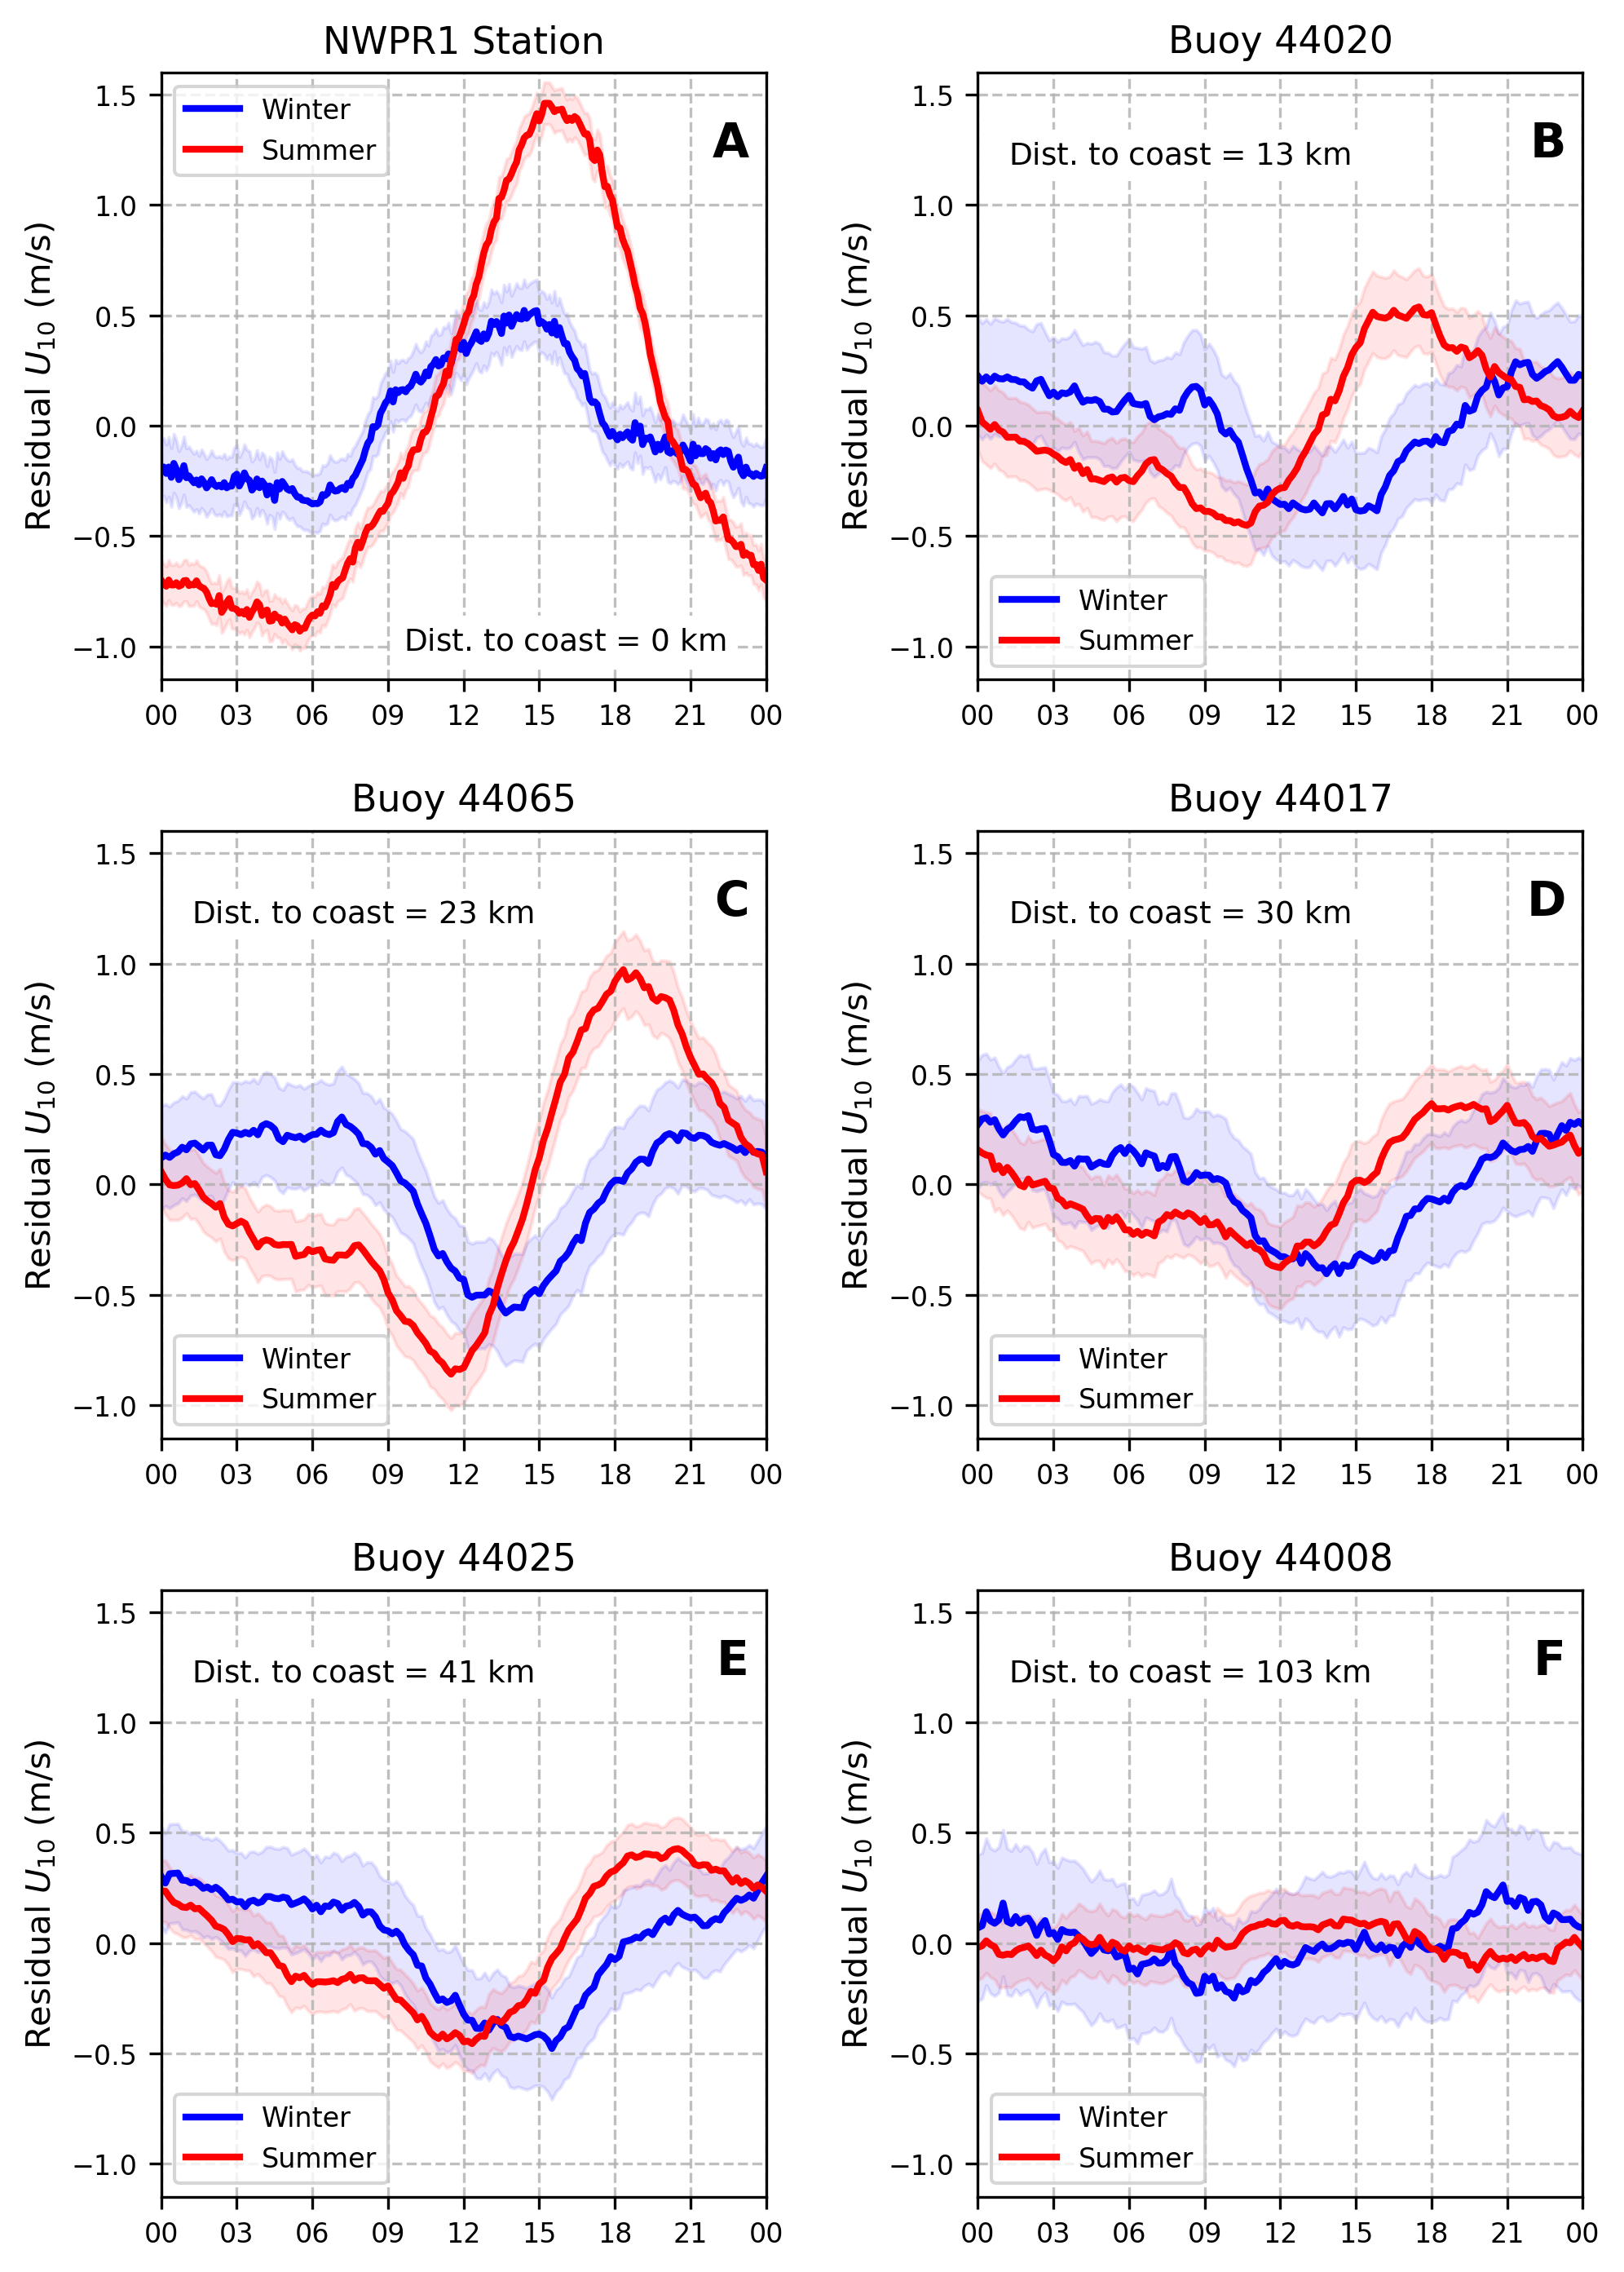
\includegraphics[width=1.\linewidth]{Figures/Chapter5/wind_diurnal_variability_residuals11.png}
%\decoRule
\caption{NDBC Buoys \& Station NWPR1 (Newport, RI) $u_{10}$ diurnal cycle for the winter and summer seasons.}
\label{fig:wind_diur_variability}
\end{figure}



\begin{figure}[H]
\centering
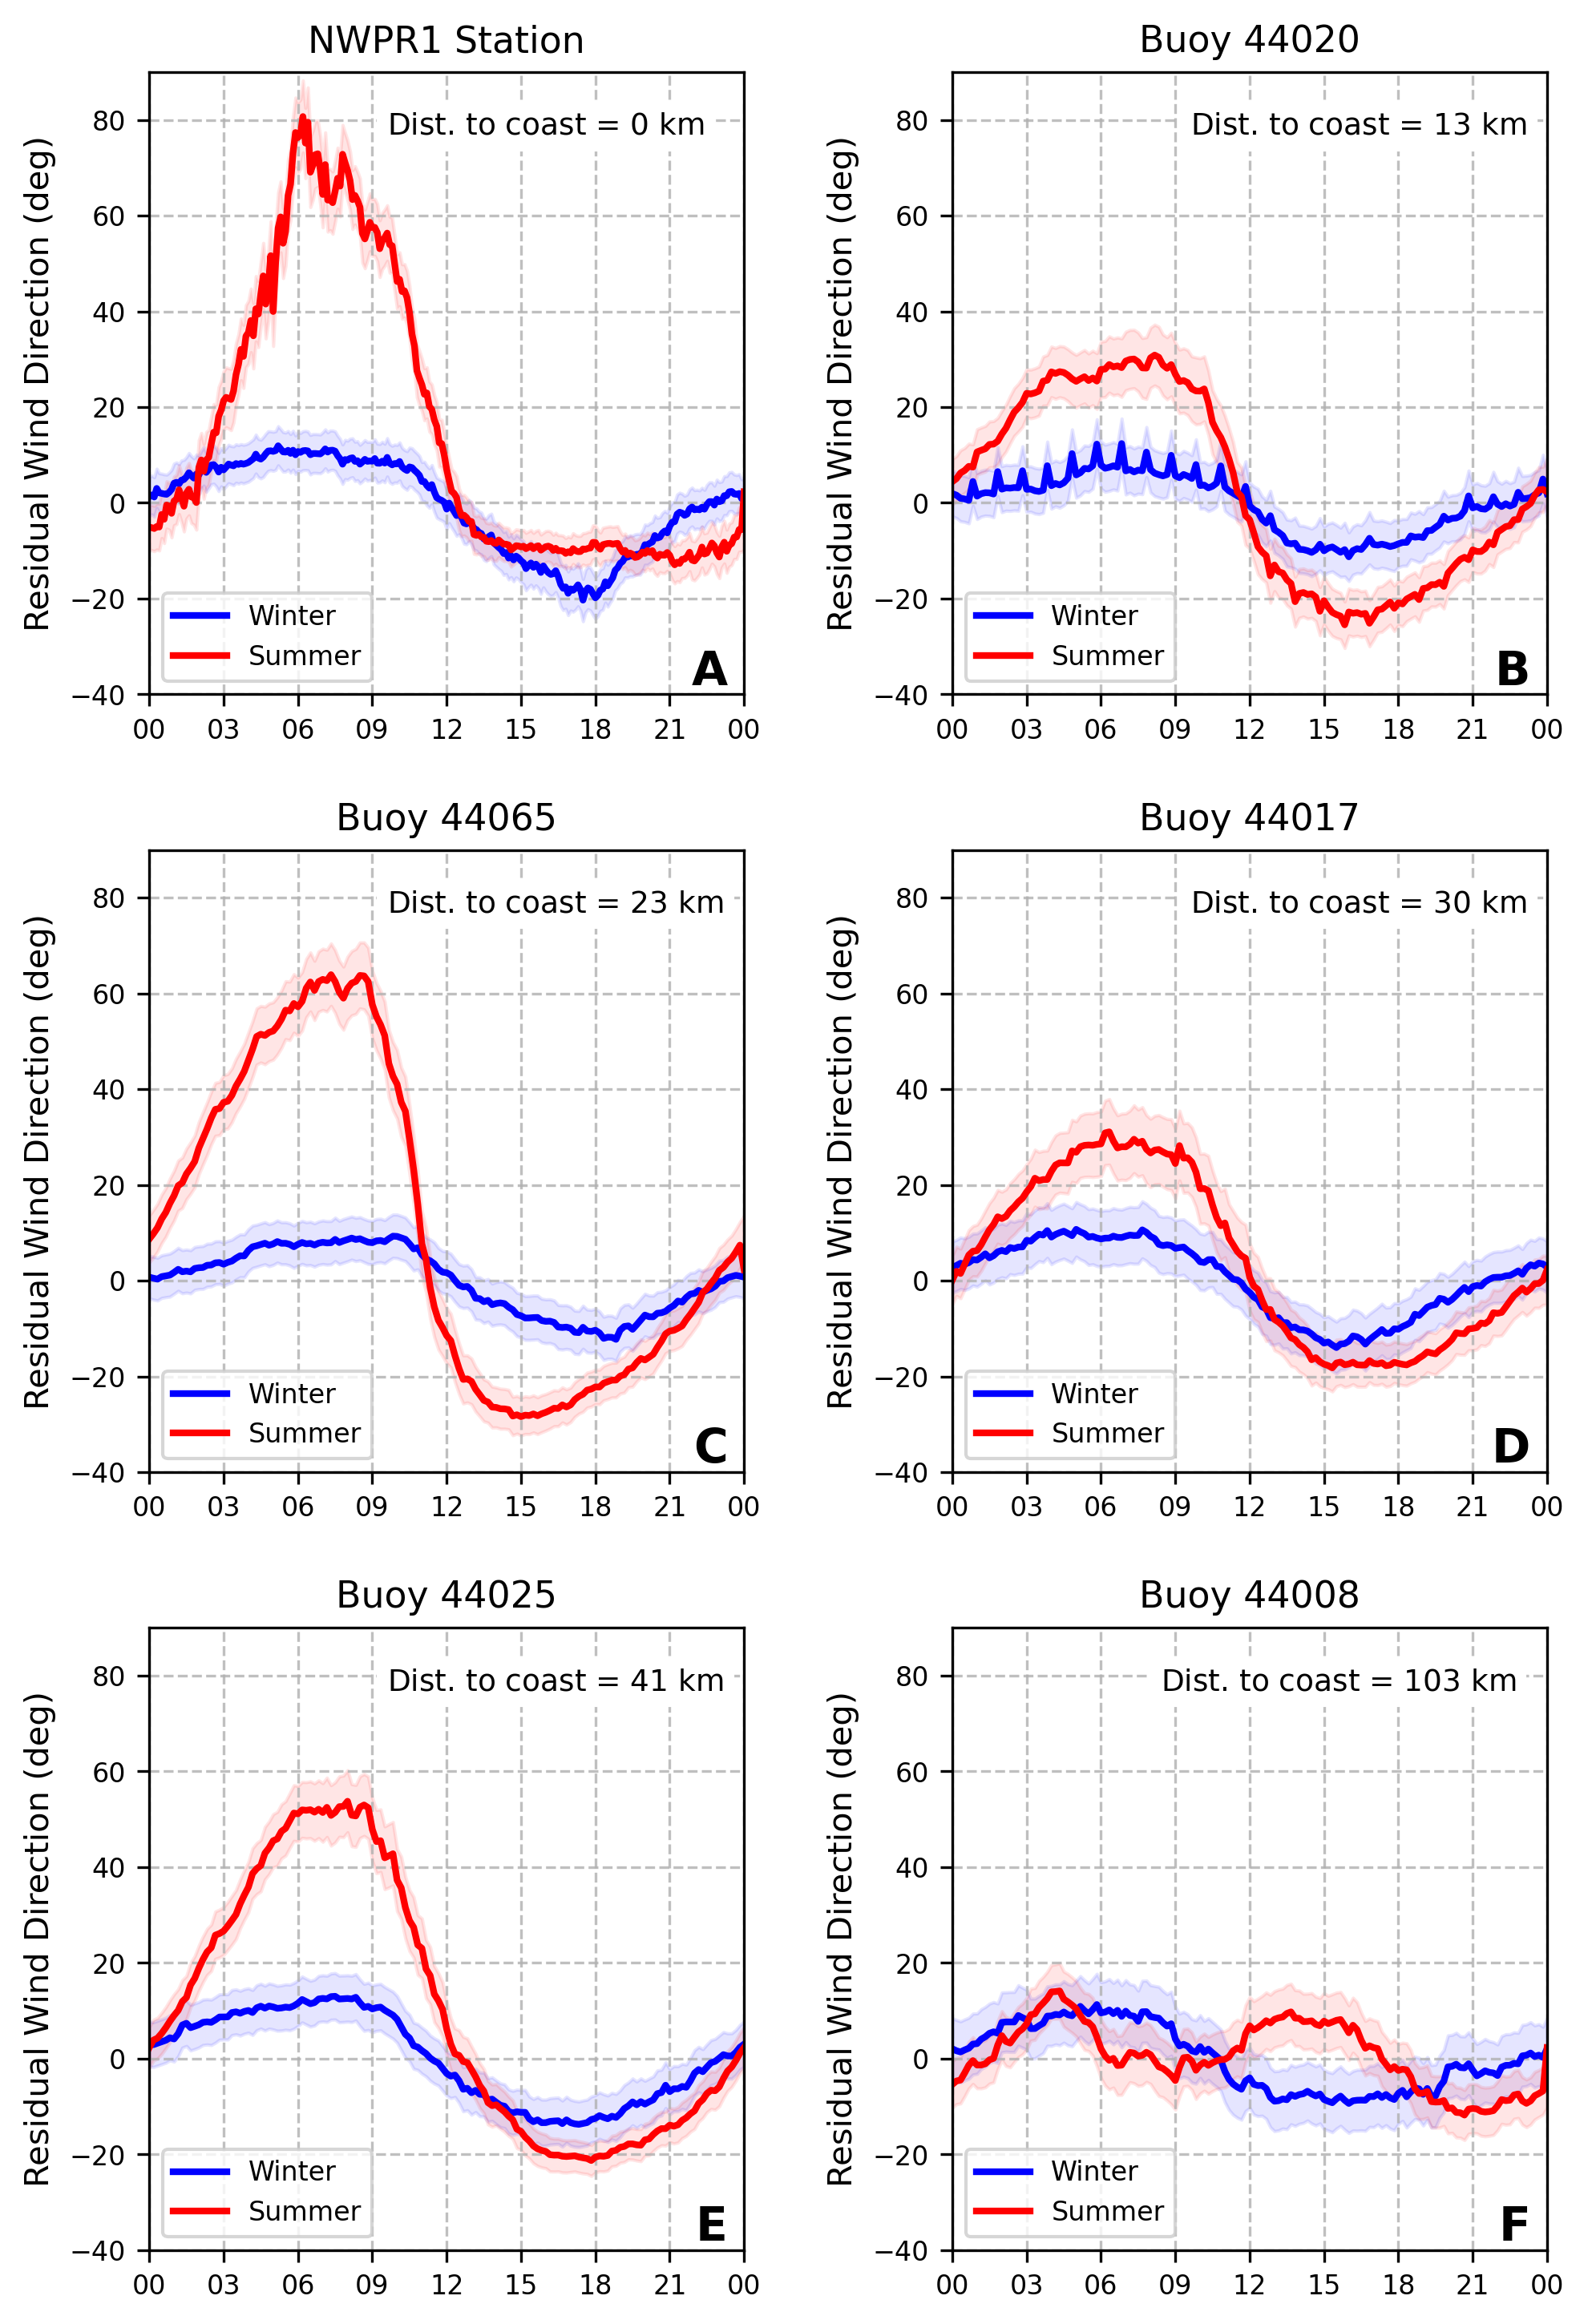
\includegraphics[width=1.\linewidth]{Figures/Chapter5/wind_dir_diurnal_variability_residuals11.png}
%\decoRule
\caption{NDBC Buoys \& Station NWPR1 (Newport, RI) wind direction diurnal cycle for the winter and summer seasons.}
\label{fig:wind_dir_diur_variability}
\end{figure}


The diurnal cycles of the buoys located kilometers offshore reveal different attributes. The western part of the region presents the highest diurnal range, specifically at the coastal buoy 44065 location, 23 kilometers from the closest shore and southwest of Long Island. Therefore, both the proximity to land and the topography surrounding each buoy's location has to be considered. As we move further off the coast and to the eastern part of the region, the diurnal range differences for $u_{10}$ and wind direction between summer and winter are not as significant as for station NWPR1. The uncertainty of the estimations also becomes higher. Besides, the WS diurnal cycle is not synchronous with the wind direction diurnal cycle. Generally, the lowest WS values are identified between 10:30 AM and 12:30 PM during the summer and the highest in the evening between 5:30 PM and 8:30 PM. On the other hand, minimum WS values are found during winter between 1:30 PM and 3:30 PM and the maximum in the early morning hours. There are also local wind speed maxima between 6:00 and 9:00 AM, which are apparent in Figures \ref{fig:wind_diur_variability}B and \ref{fig:wind_diur_variability}C. The diurnal range is more extensive during summer, and it can reach up to 2m/s. Maximum WS values are observed earlier at stations with closer proximity to the land.  On the contrary, buoys' winter diurnal cycle is almost the reverse of the NWPR1 station. Specifically, buoys' minimum WS values are reported between 12:00 and 3:00 PM, the same hours of maximum WS observed on land. In contrast, the wind direction's diurnal cycle for each location coincides.

However, the above description does not include buoy 44008. Figures~\ref{fig:wind_diur_variability}F and \ref{fig:wind_dir_diur_variability}F confirm that the advective effects do not appear to influence locations 100 kilometers off the closest coast, where the diurnal range is almost negligible. Therefore, it may be concluded that generally, the diurnal variability has to be considered at distances less than 40 kilometers from the land. Still, it becomes weak at 100 kilometers or more offshore, especially on the eastern side of SNE.

Finally, the diurnal variability of the wind does not affect the wave climate significantly. The diurnal range of the SWH is in the order of centimeters (not shown here). Besides, we did not identify any significant influence on the directional spectra's diurnal variability for buoy 44097.



\begin{figure}[H]
\centering
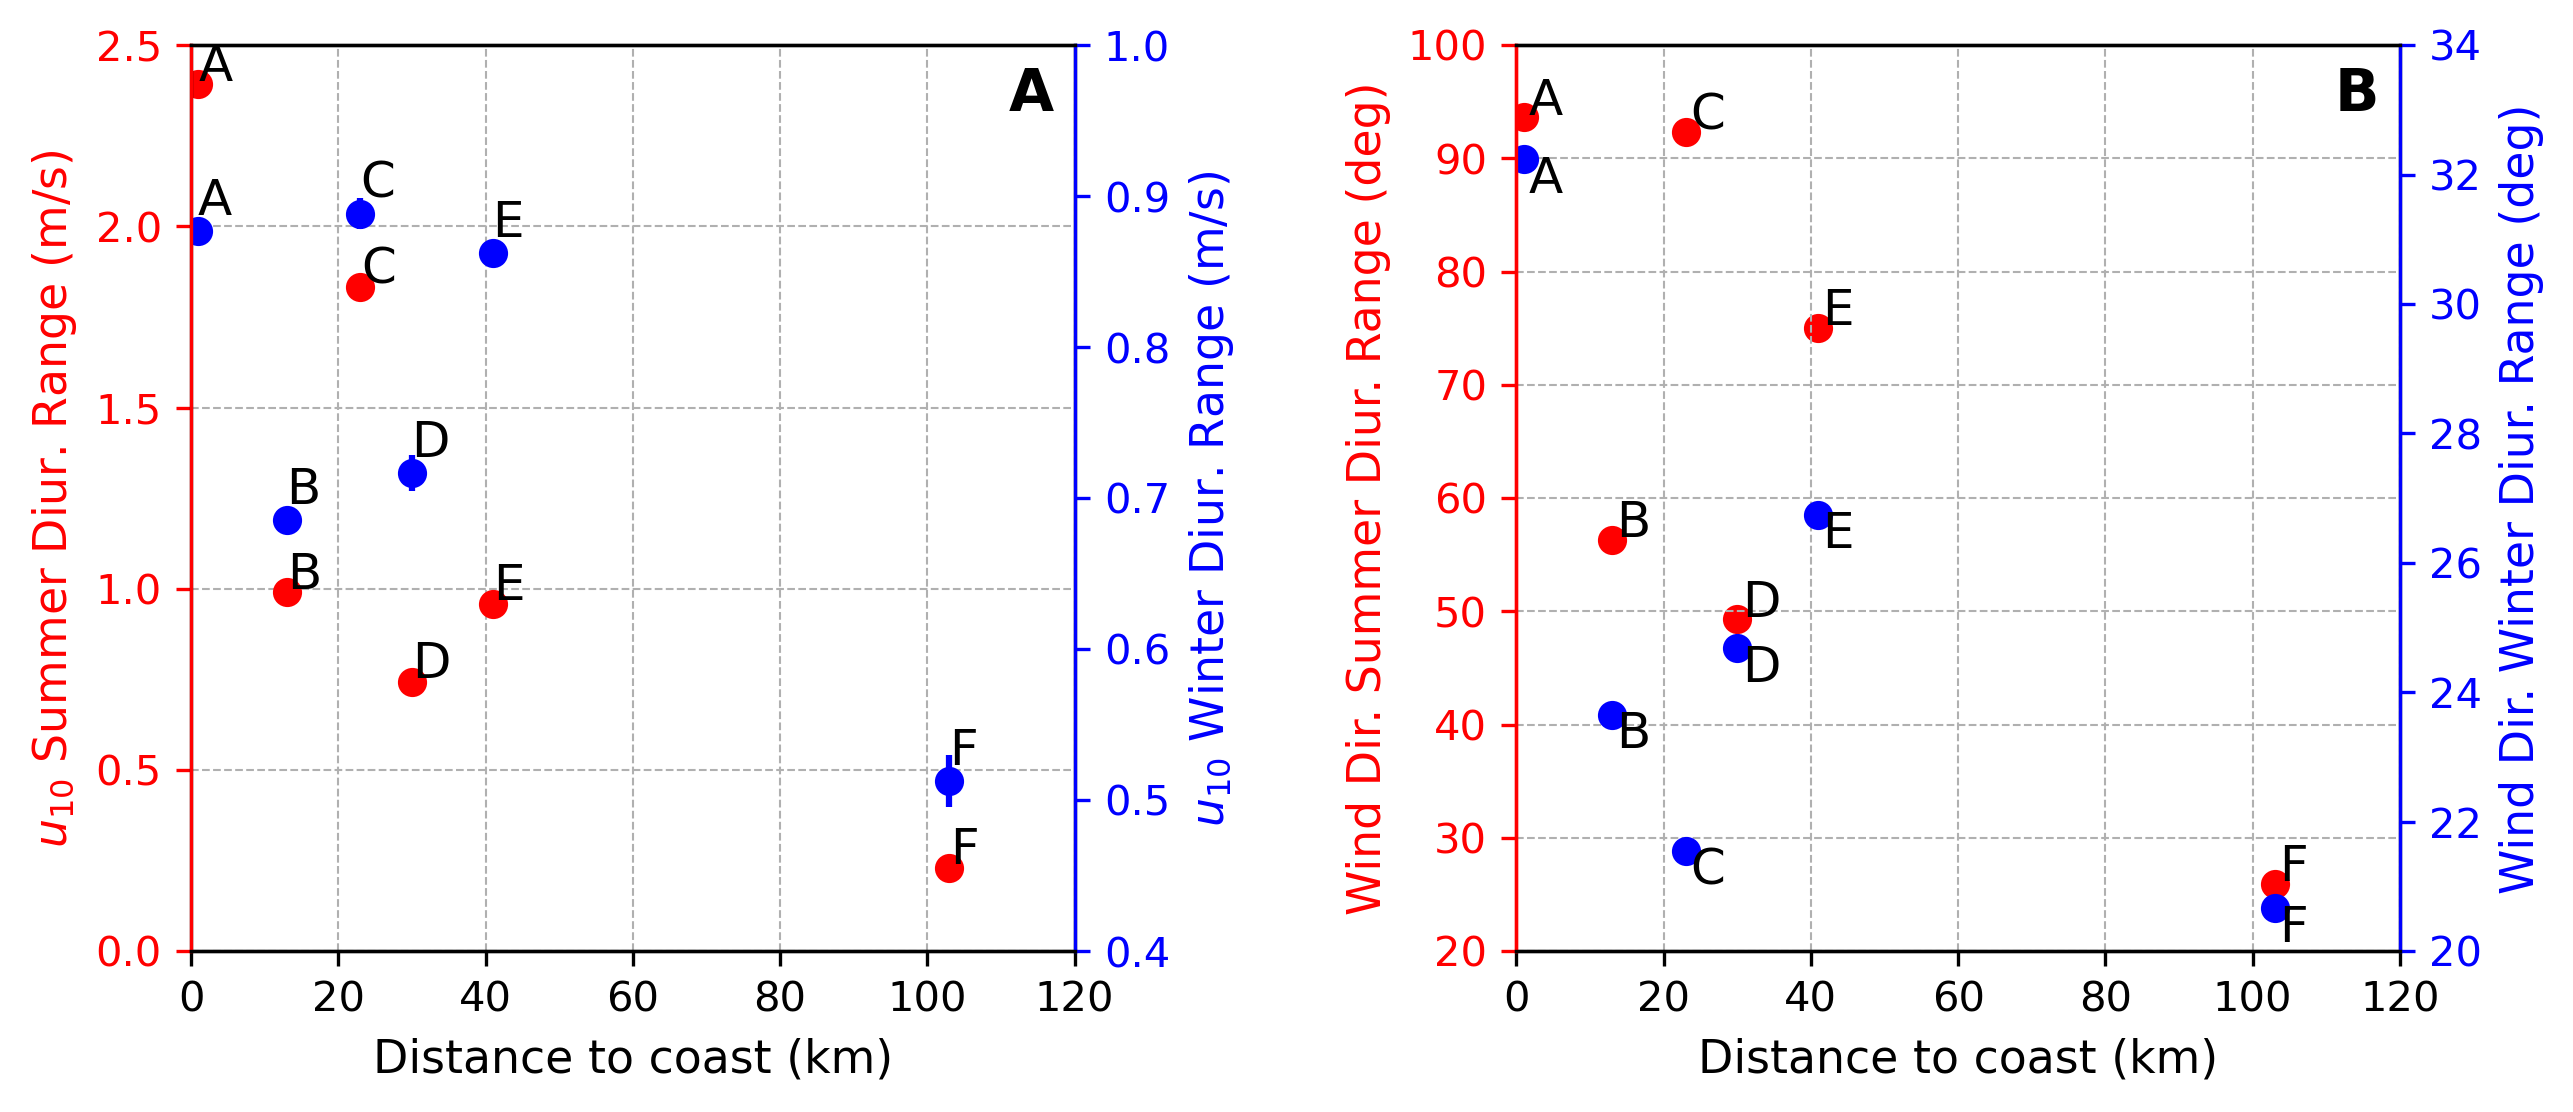
\includegraphics[width=0.95\linewidth]{Figures/Chapter5/wind_diurnal_range1.png}
%\decoRule
\caption{NDBC Buoys and NWPR1 station wind speed and direction diurnal range with respect to their distance from the closest coast.}
\label{fig:wind_diurnal_range}
\end{figure}

\pagebreak

\subsection{Seasonal Variability}\label{seasonal_variability}

The seasonal variability of both the $H_{s}$ and the $u_{10}$ will be characterized in this study for SNE, a North Atlantic coastal region, using buoy data. Young \cite{ Young1999c} documented the North Atlantic wind and wave climate's strong seasonal trends using altimeter data and numerical models. He also emphasized that the extended NDBC buoy network is suitable for regional studies. 


Figure~\ref{fig:buoy_wind_seasonality} shows the $u_{10}$ seasonal variability for six of the available buoys, including the daily mean values, their 25th, 75th percentiles, and a monthly lowpass filter to visualize the seasonality. Both Figure~\ref{fig:buoy_wind_seasonality} and the average $u_{10}$ values available in tables \ref{tab:wind_distribution_winter},  \ref{tab:wind_distribution_summer} display that the seasonal variability ranges from 2m/s for the sheltered buoy 44020 to almost 4.5 m/s for the open ocean buoy 44008. Figure~\ref{fig:buoy_wave_seasonality} shows similar results for the $H_{s}$. Buoys 44020 and 44065 that are closer to the coast show almost zero seasonal variability. Buoy 44039, located in the Long Island Sound, shows stronger seasonal variability with lower WS values on average than buoy 44020, even if they have the same distance to the coast. On the contrary, at over 100 kilometers from the coast, buoy 44008 presents a strong seasonal variability of approximately 1.3 meters on average. This difference is only partly explained by the direct influence of the wind on the sea surface. We show in \ref{inverse_wave_age} that the percentage of purely wind waves at the buoy 44008 location is small, especially during the summer season, and the opposite applies for the sheltered buoy 44020. Therefore, the strong seasonal variability in the open ocean buoy's location is also connected with the North Atlantic variability trend described by Young. In contrast, buoy 44020 is located 13 kilometers from the closest coast, where there is a low presence of swell waves due to topography. Finally, we can identify local minima during the first days of December for both $u_{10}$ and $H_{s}$ (Figure~\ref{fig:buoy_wave_seasonality}F) and also local $H_{s}$ maxima between July and August.





\begin{figure}[H]
\centering
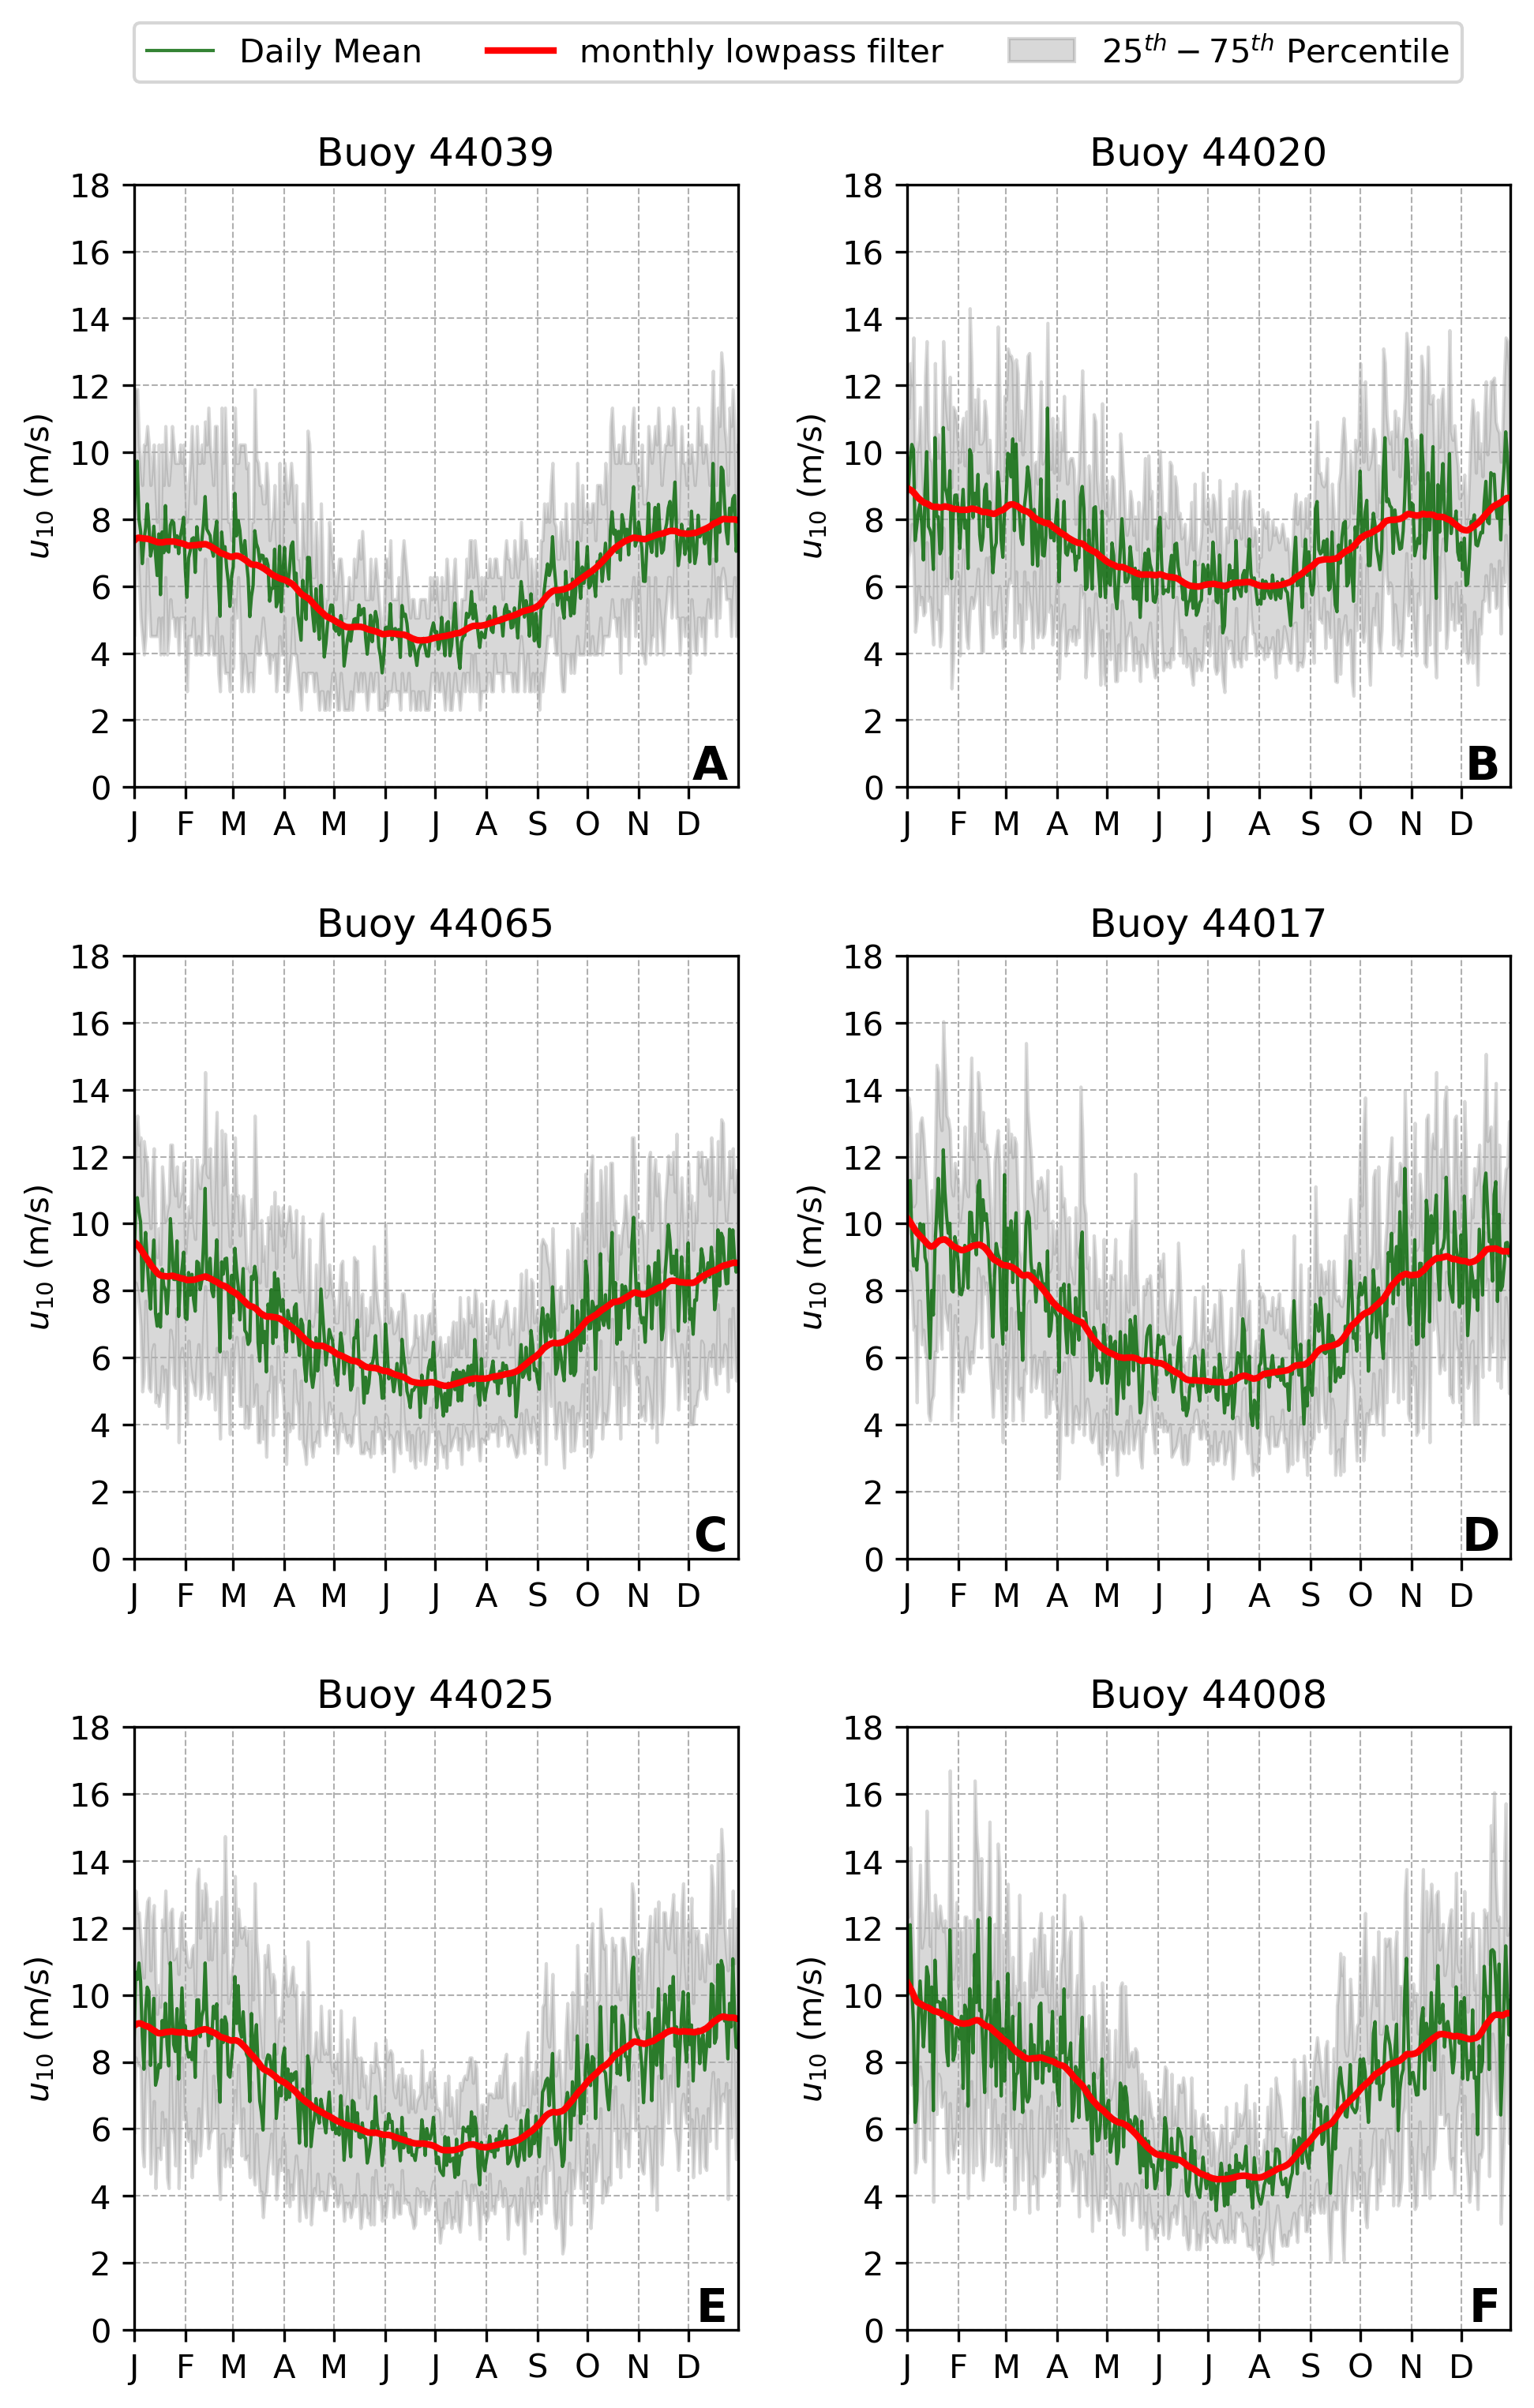
\includegraphics[width=0.95\linewidth]{Figures/Chapter5/buoys_wind_seasonal_qt1.png}
%\decoRule
\caption{Buoy $u_{10}$ seasonal variability}
\label{fig:buoy_wind_seasonality}
\end{figure}


\begin{figure}[H]
\centering
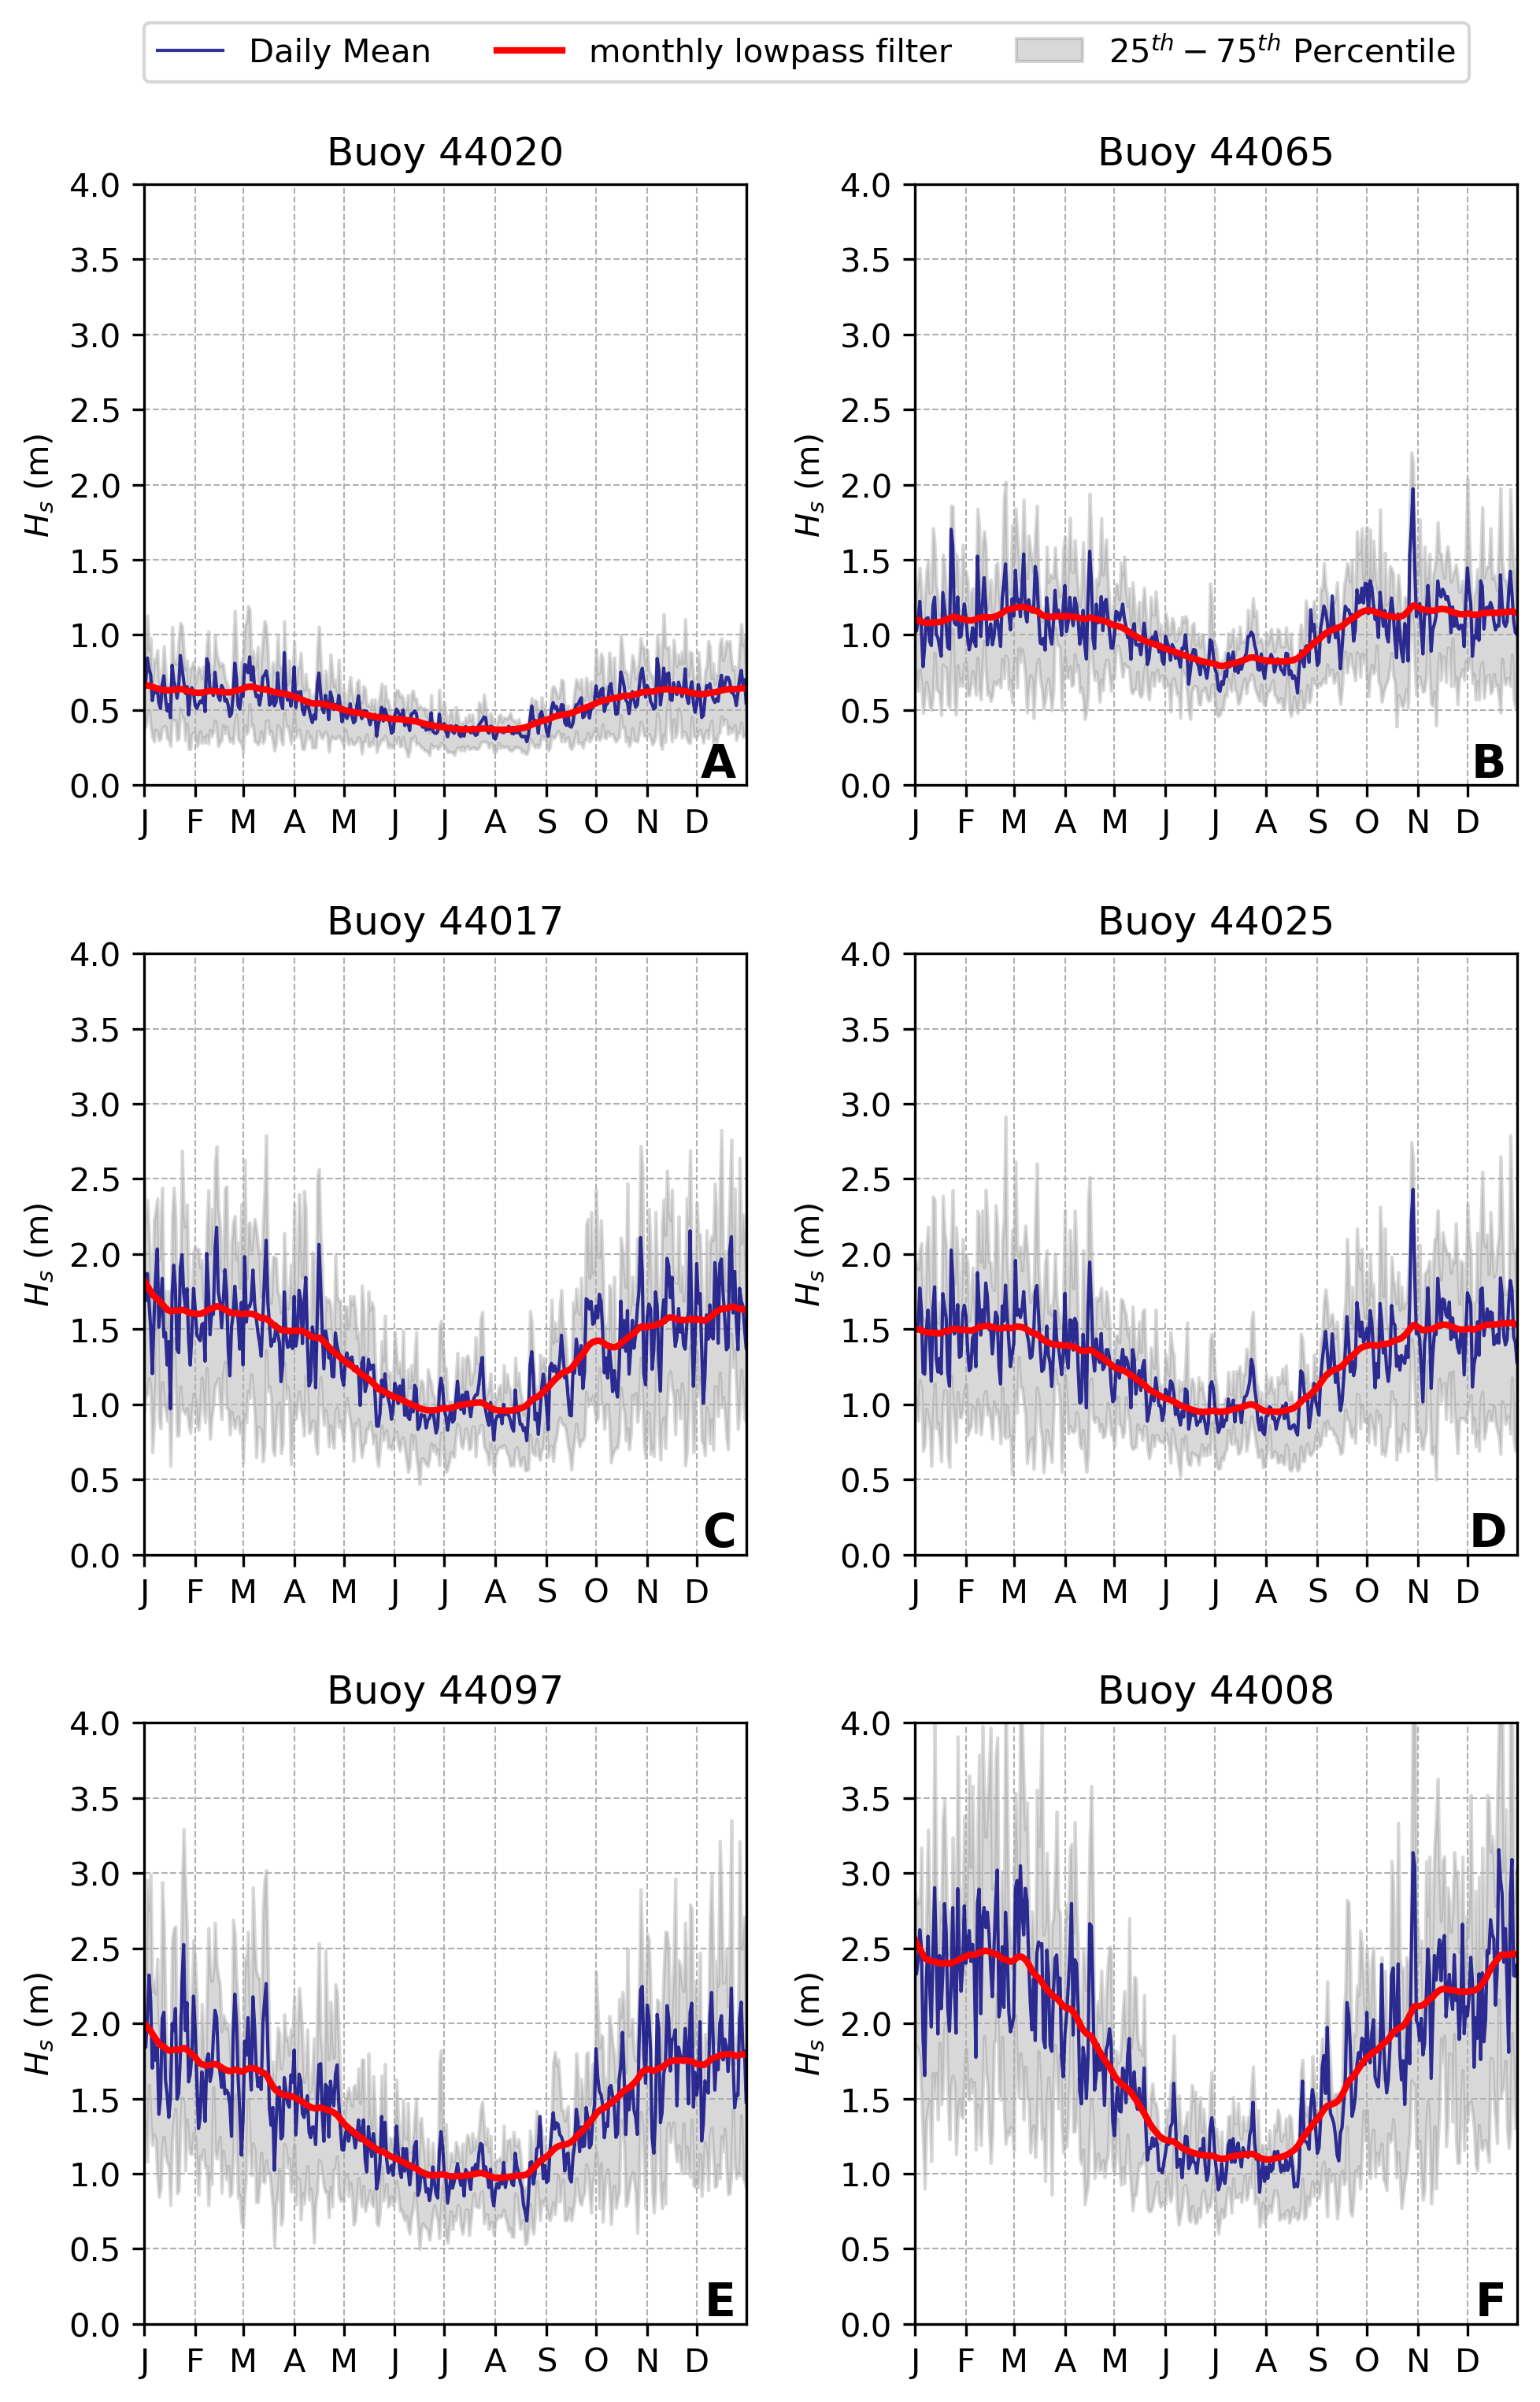
\includegraphics[width=0.95\linewidth]{Figures/Chapter5/buoys_wave_seasonal_qt1.png}
%\decoRule
\caption{Buoy $H_{s}$ seasonal variability}
\label{fig:buoy_wave_seasonality}
\end{figure}



\subsection{Interannual Variability}

The interannual variability is essential for detecting anomalies, trends, and the representation of climatic averages. Due to gaps in the buoy time series, months with less than 50\% of data availability were discarded. 



\begin{figure}[H]
\centering
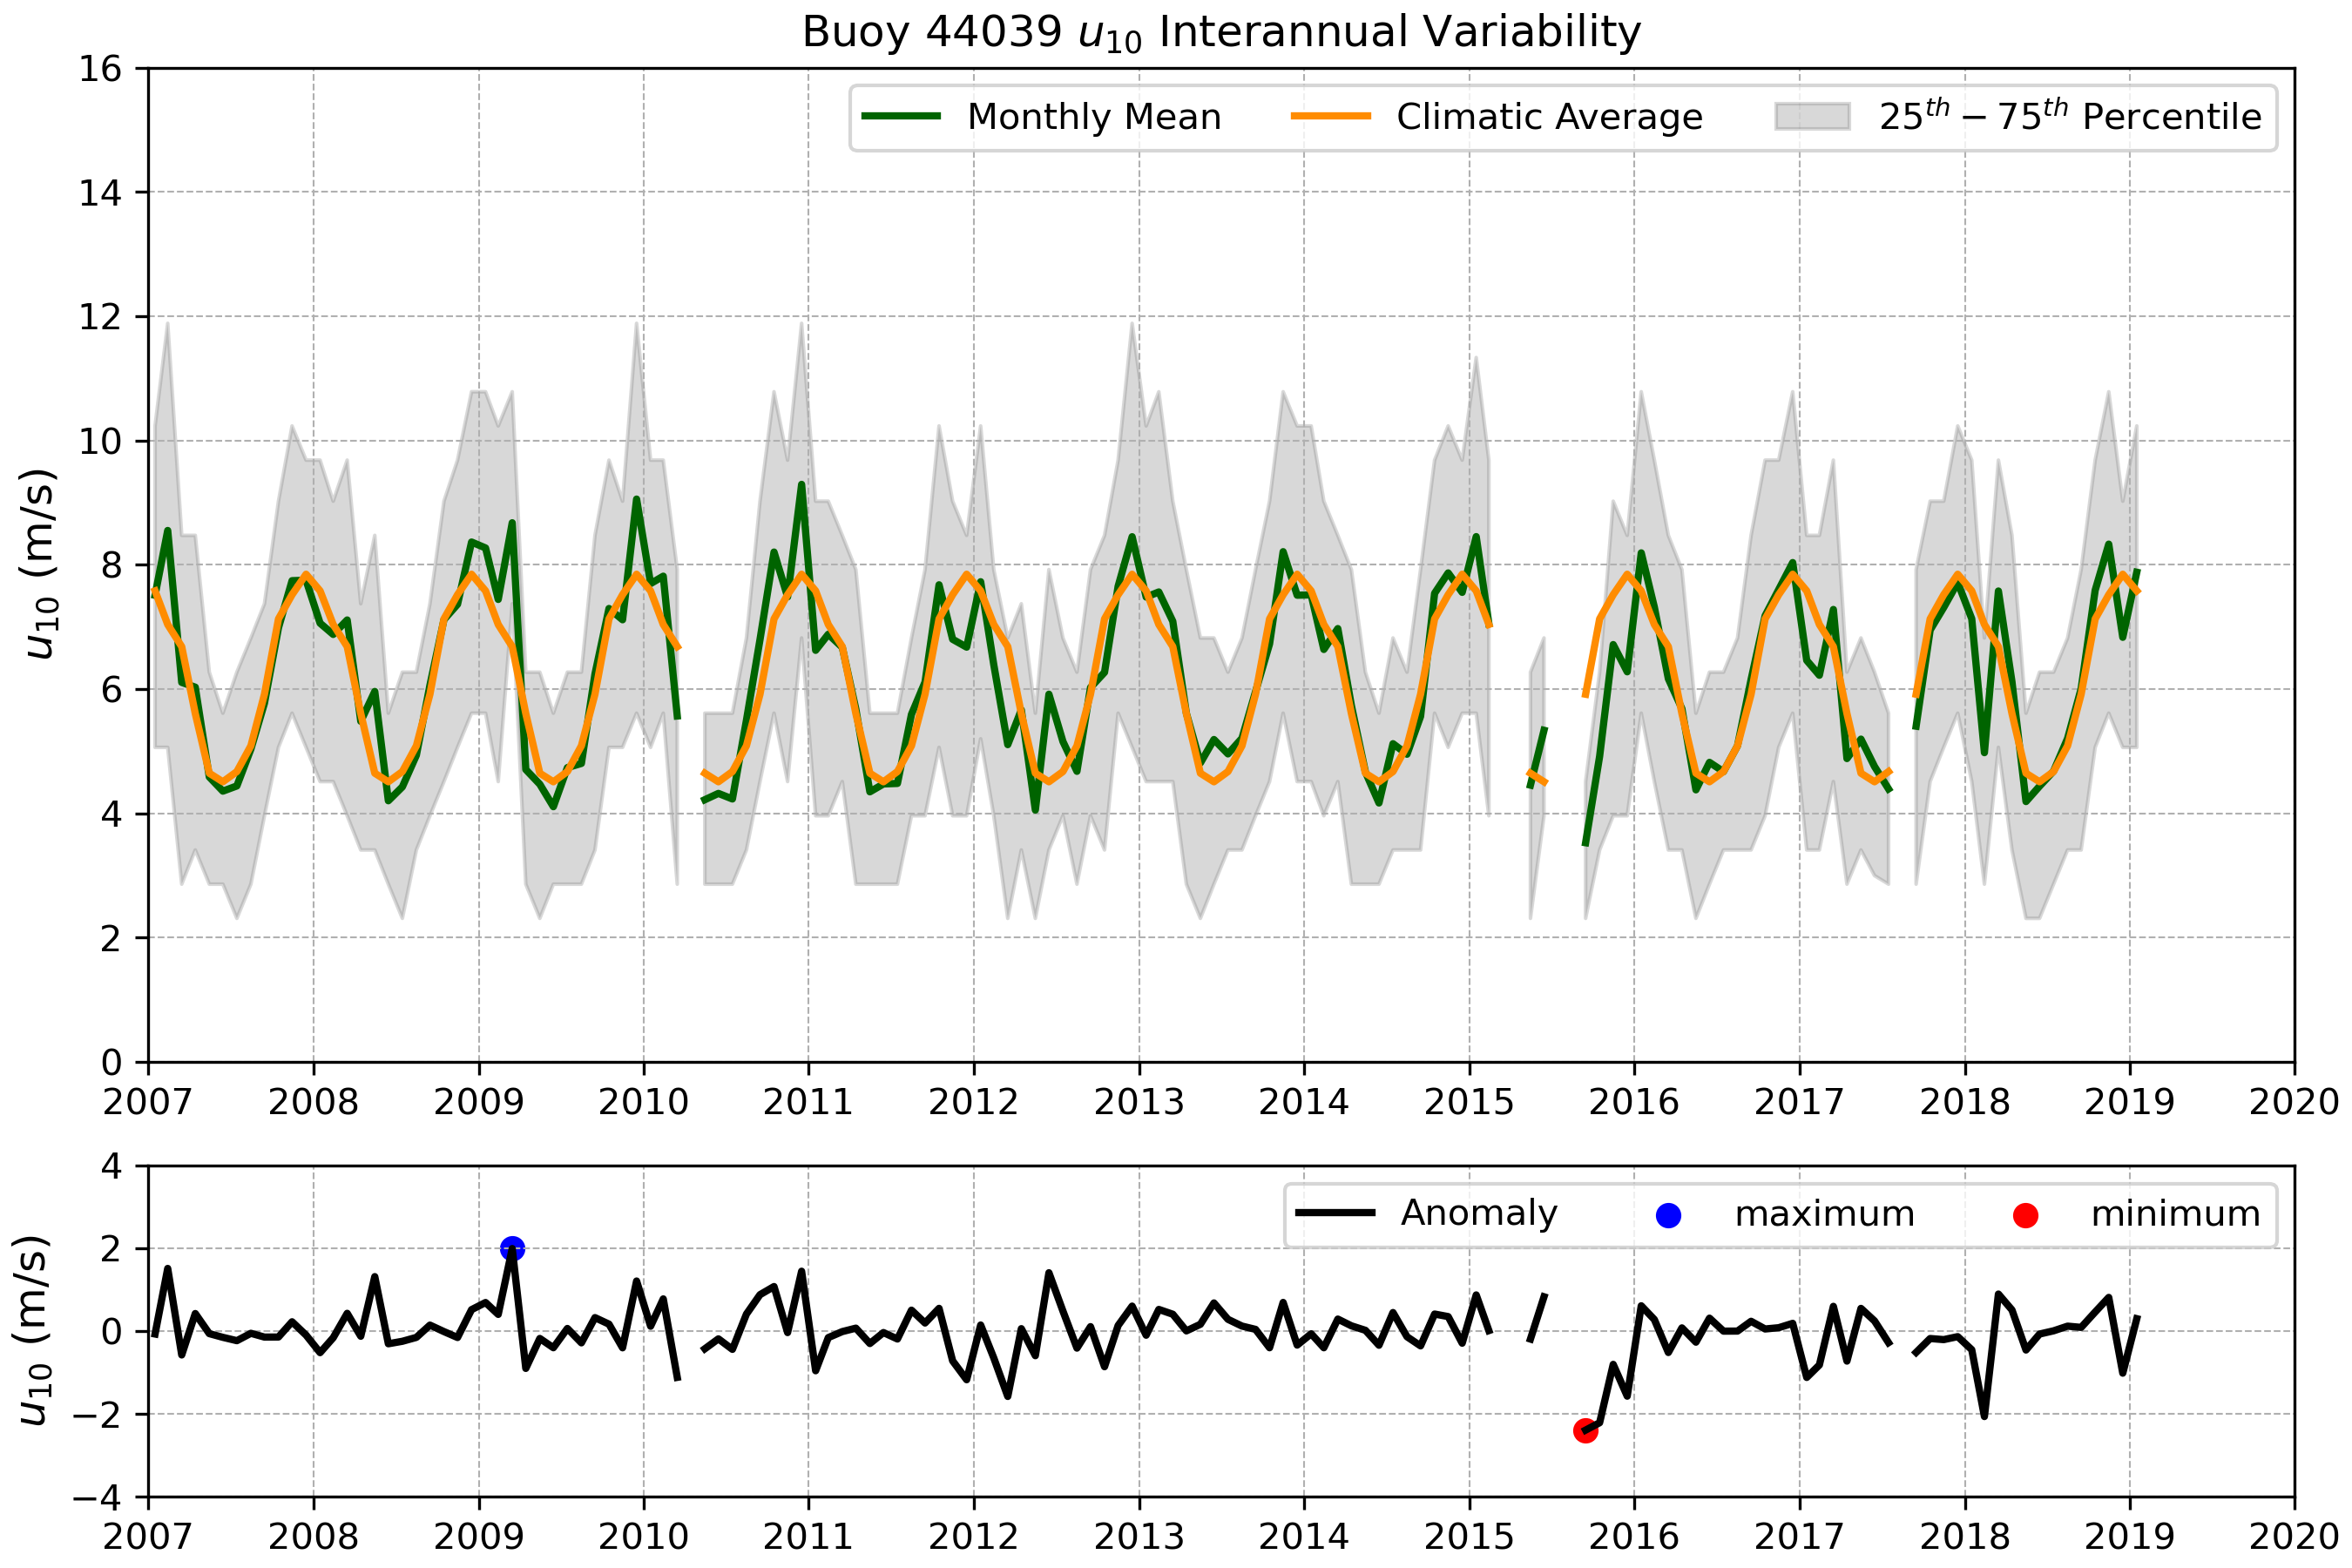
\includegraphics[width=0.83\linewidth]{Figures/Chapter5/b44039_interranual_anomaly.png}
%\decoRule
\caption{Buoy 44039 $u_{10}$ interannual variability including monthly mean values, 25th and 75th percentiles, climatic average and monthly anomalies.}
\label{fig:b44039_wind_inter}
\end{figure}


\begin{figure}[H]
\centering
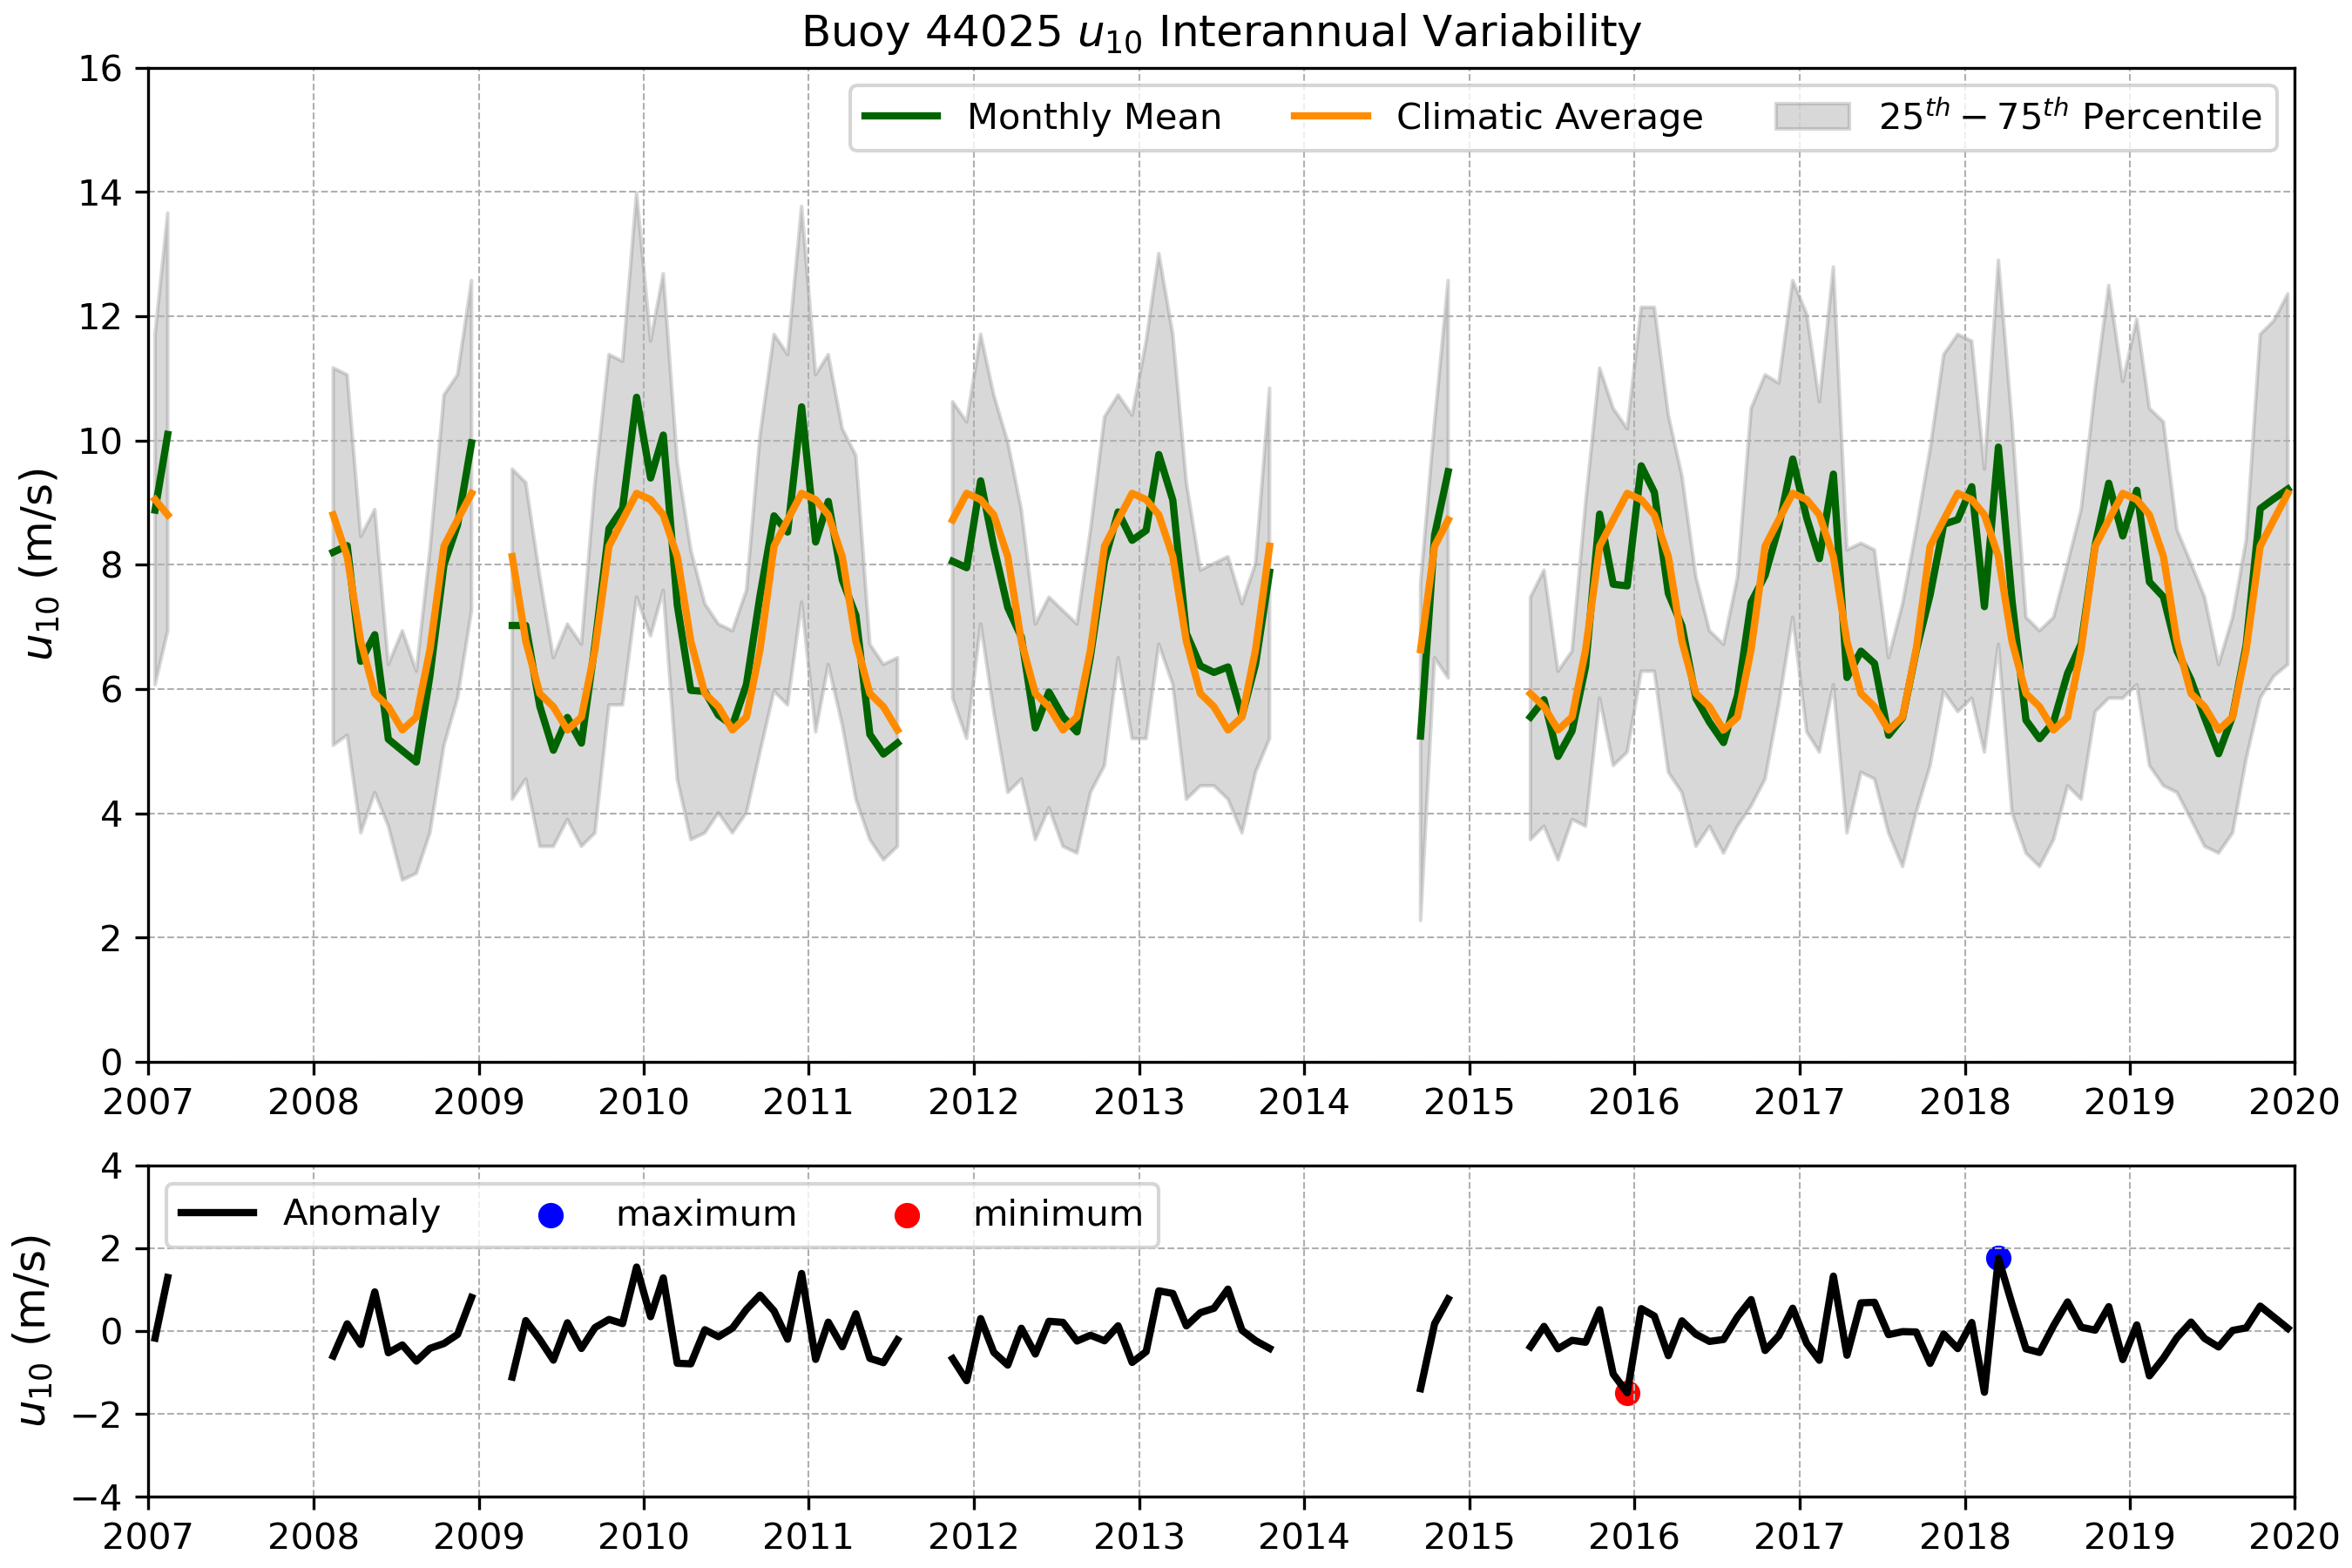
\includegraphics[width=0.83\linewidth]{Figures/Chapter5/b44025_interranual_anomaly.png}
%\decoRule
\caption{Buoy 44025 $u_{10}$ interannual variability including monthly mean values, 25th and 75th percentiles, climatic average and monthly anomalies.}
\label{fig:b44025_wind_inter}
\end{figure}


Statistically significant trends were not identified for $H_{s}$ and $u_{10}$ both for the winter and summer seasons. Two methods were used: linear regression analysis and calculating the regression slope and the Mann-Kendall and seasonal Mann-Kendall trend test \cite{Hussain2019}.



\begin{figure}[H]
\centering
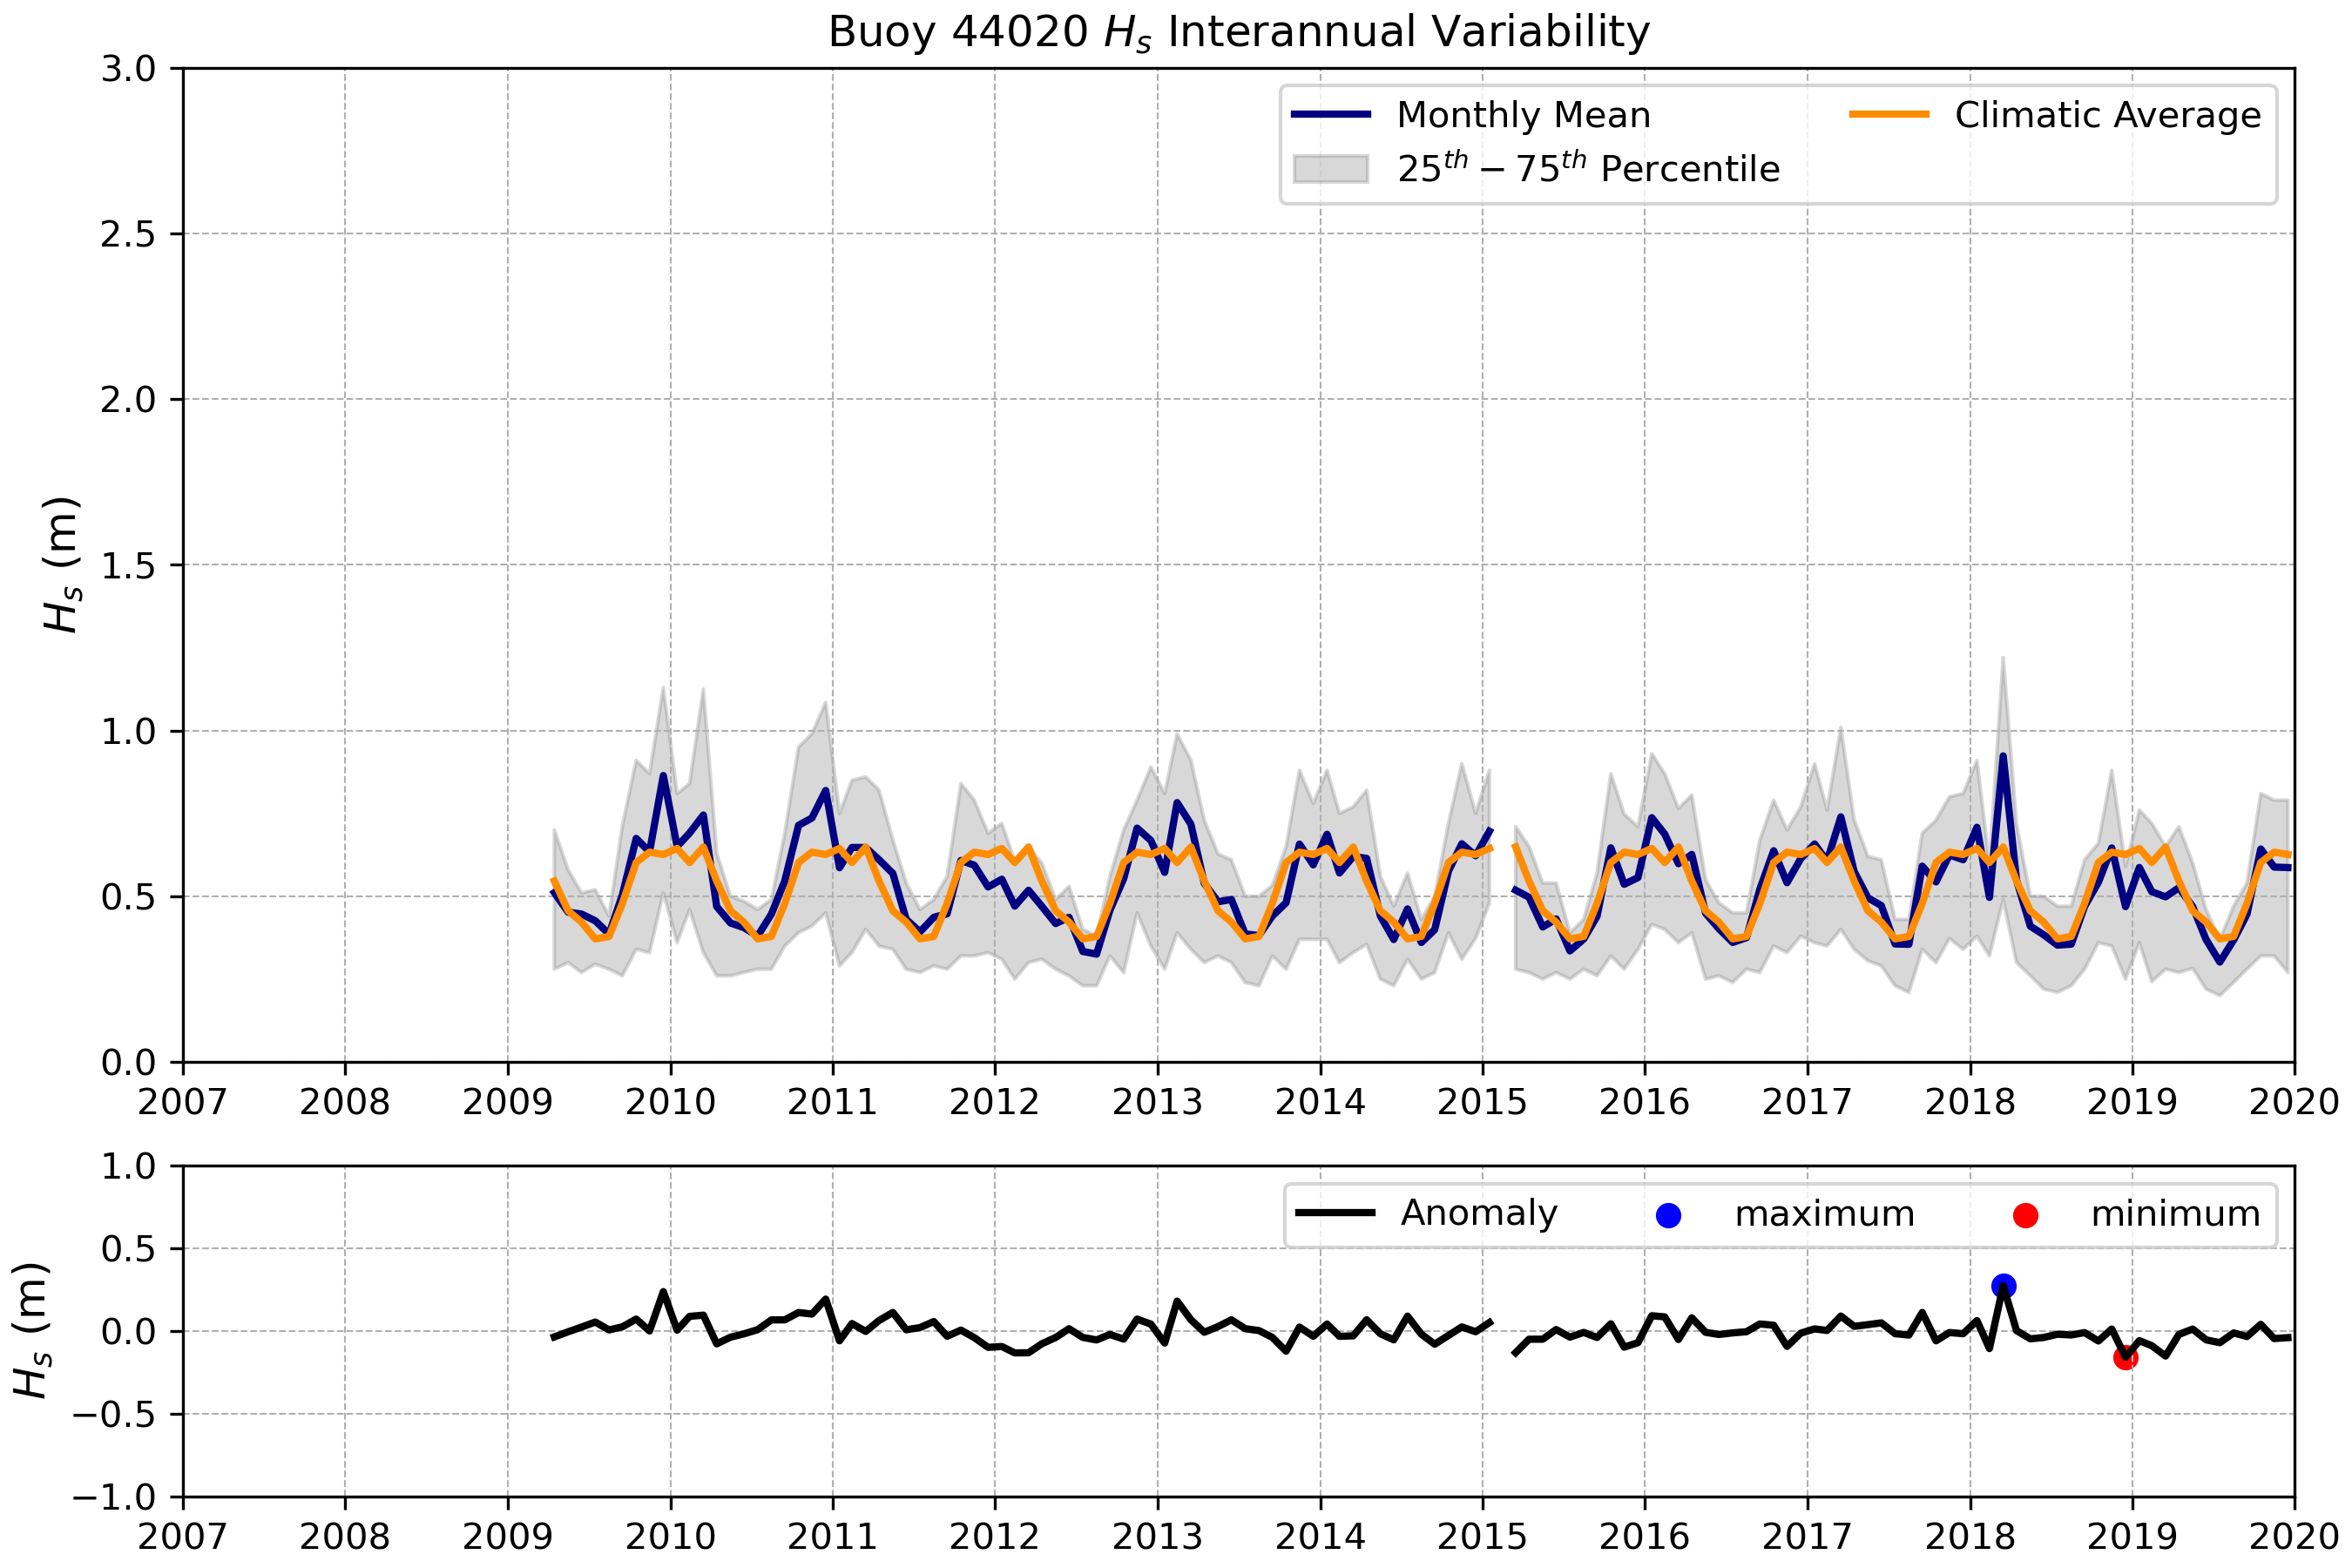
\includegraphics[width=0.83\linewidth]{Figures/Chapter5/b44020_interranual_anomaly_hs.png}
%\decoRule
\caption{Buoy 44020 $u_{10}$ interannual variability including monthly mean values, 25th and 75th percentiles, climatic average and monthly anomalies.}
\label{fig:b44020_wave_inter}
\end{figure}


\begin{figure}[H]
\centering
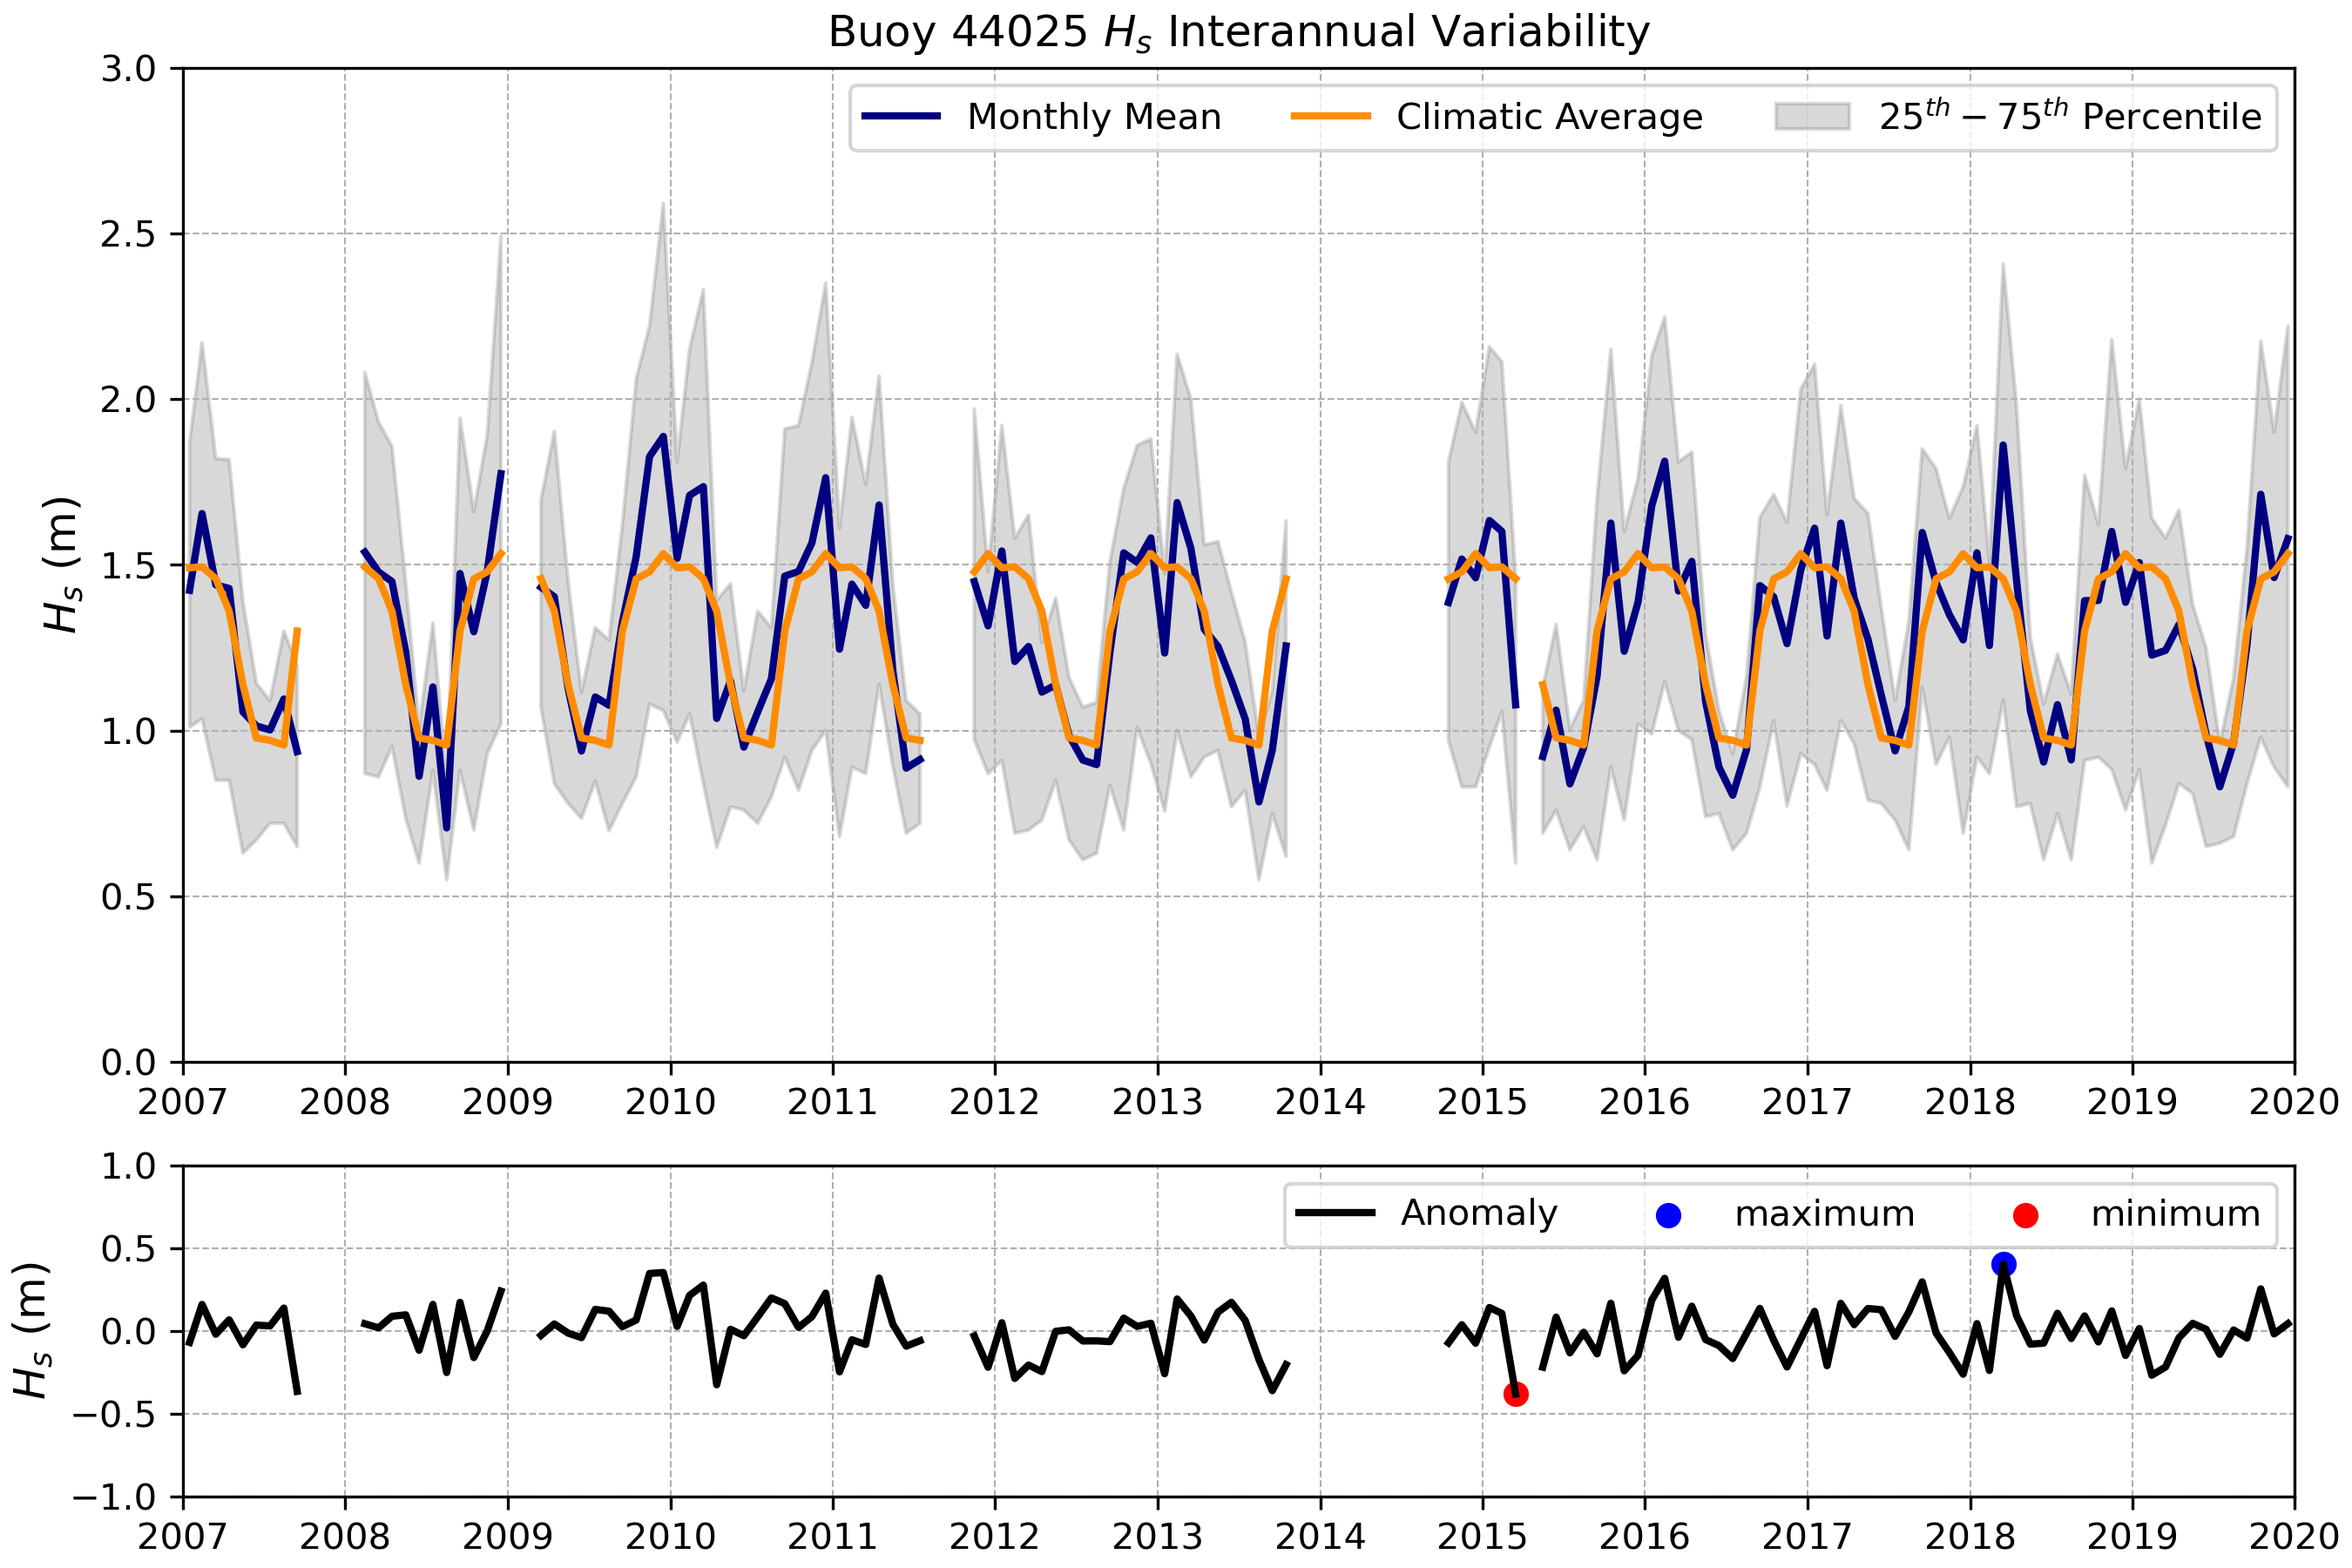
\includegraphics[width=0.83\linewidth]{Figures/Chapter5/b44025_interranual_anomaly_hs.png}
%\decoRule
\caption{Buoy 44025 $u_{10}$ interannual variability including monthly mean values, 25th and 75th percentiles, climatic average and monthly anomalies.}
\label{fig:b44025_wave_inter}
\end{figure}


Data gaps and the relatively small number of years with available data for almost all stations were limiting factors to achieve statistical significance. For completeness, the interannual variability of $H_{s}$ and $u_{10}$ for the buoys with small gaps in their time series are included in this section. In recent literature, data from long-term altimeter records and numerical models are not indicating statistically significant trends on the Northeast Atlantic coasts either \cite{Meucci2020, Timmermans2020}.

A feature that requires attention is the double peaks from late autumn to early spring, especially when considering the $H_{s}$ figures. For example, the double peaks in Figure~\ref{fig:b44097_wave_inter} can be assessed considering the monthly average wave spectrum of the same buoy in Figure~\ref{fig:monthly_dir_spectra}. 


\begin{figure}[H]
\centering
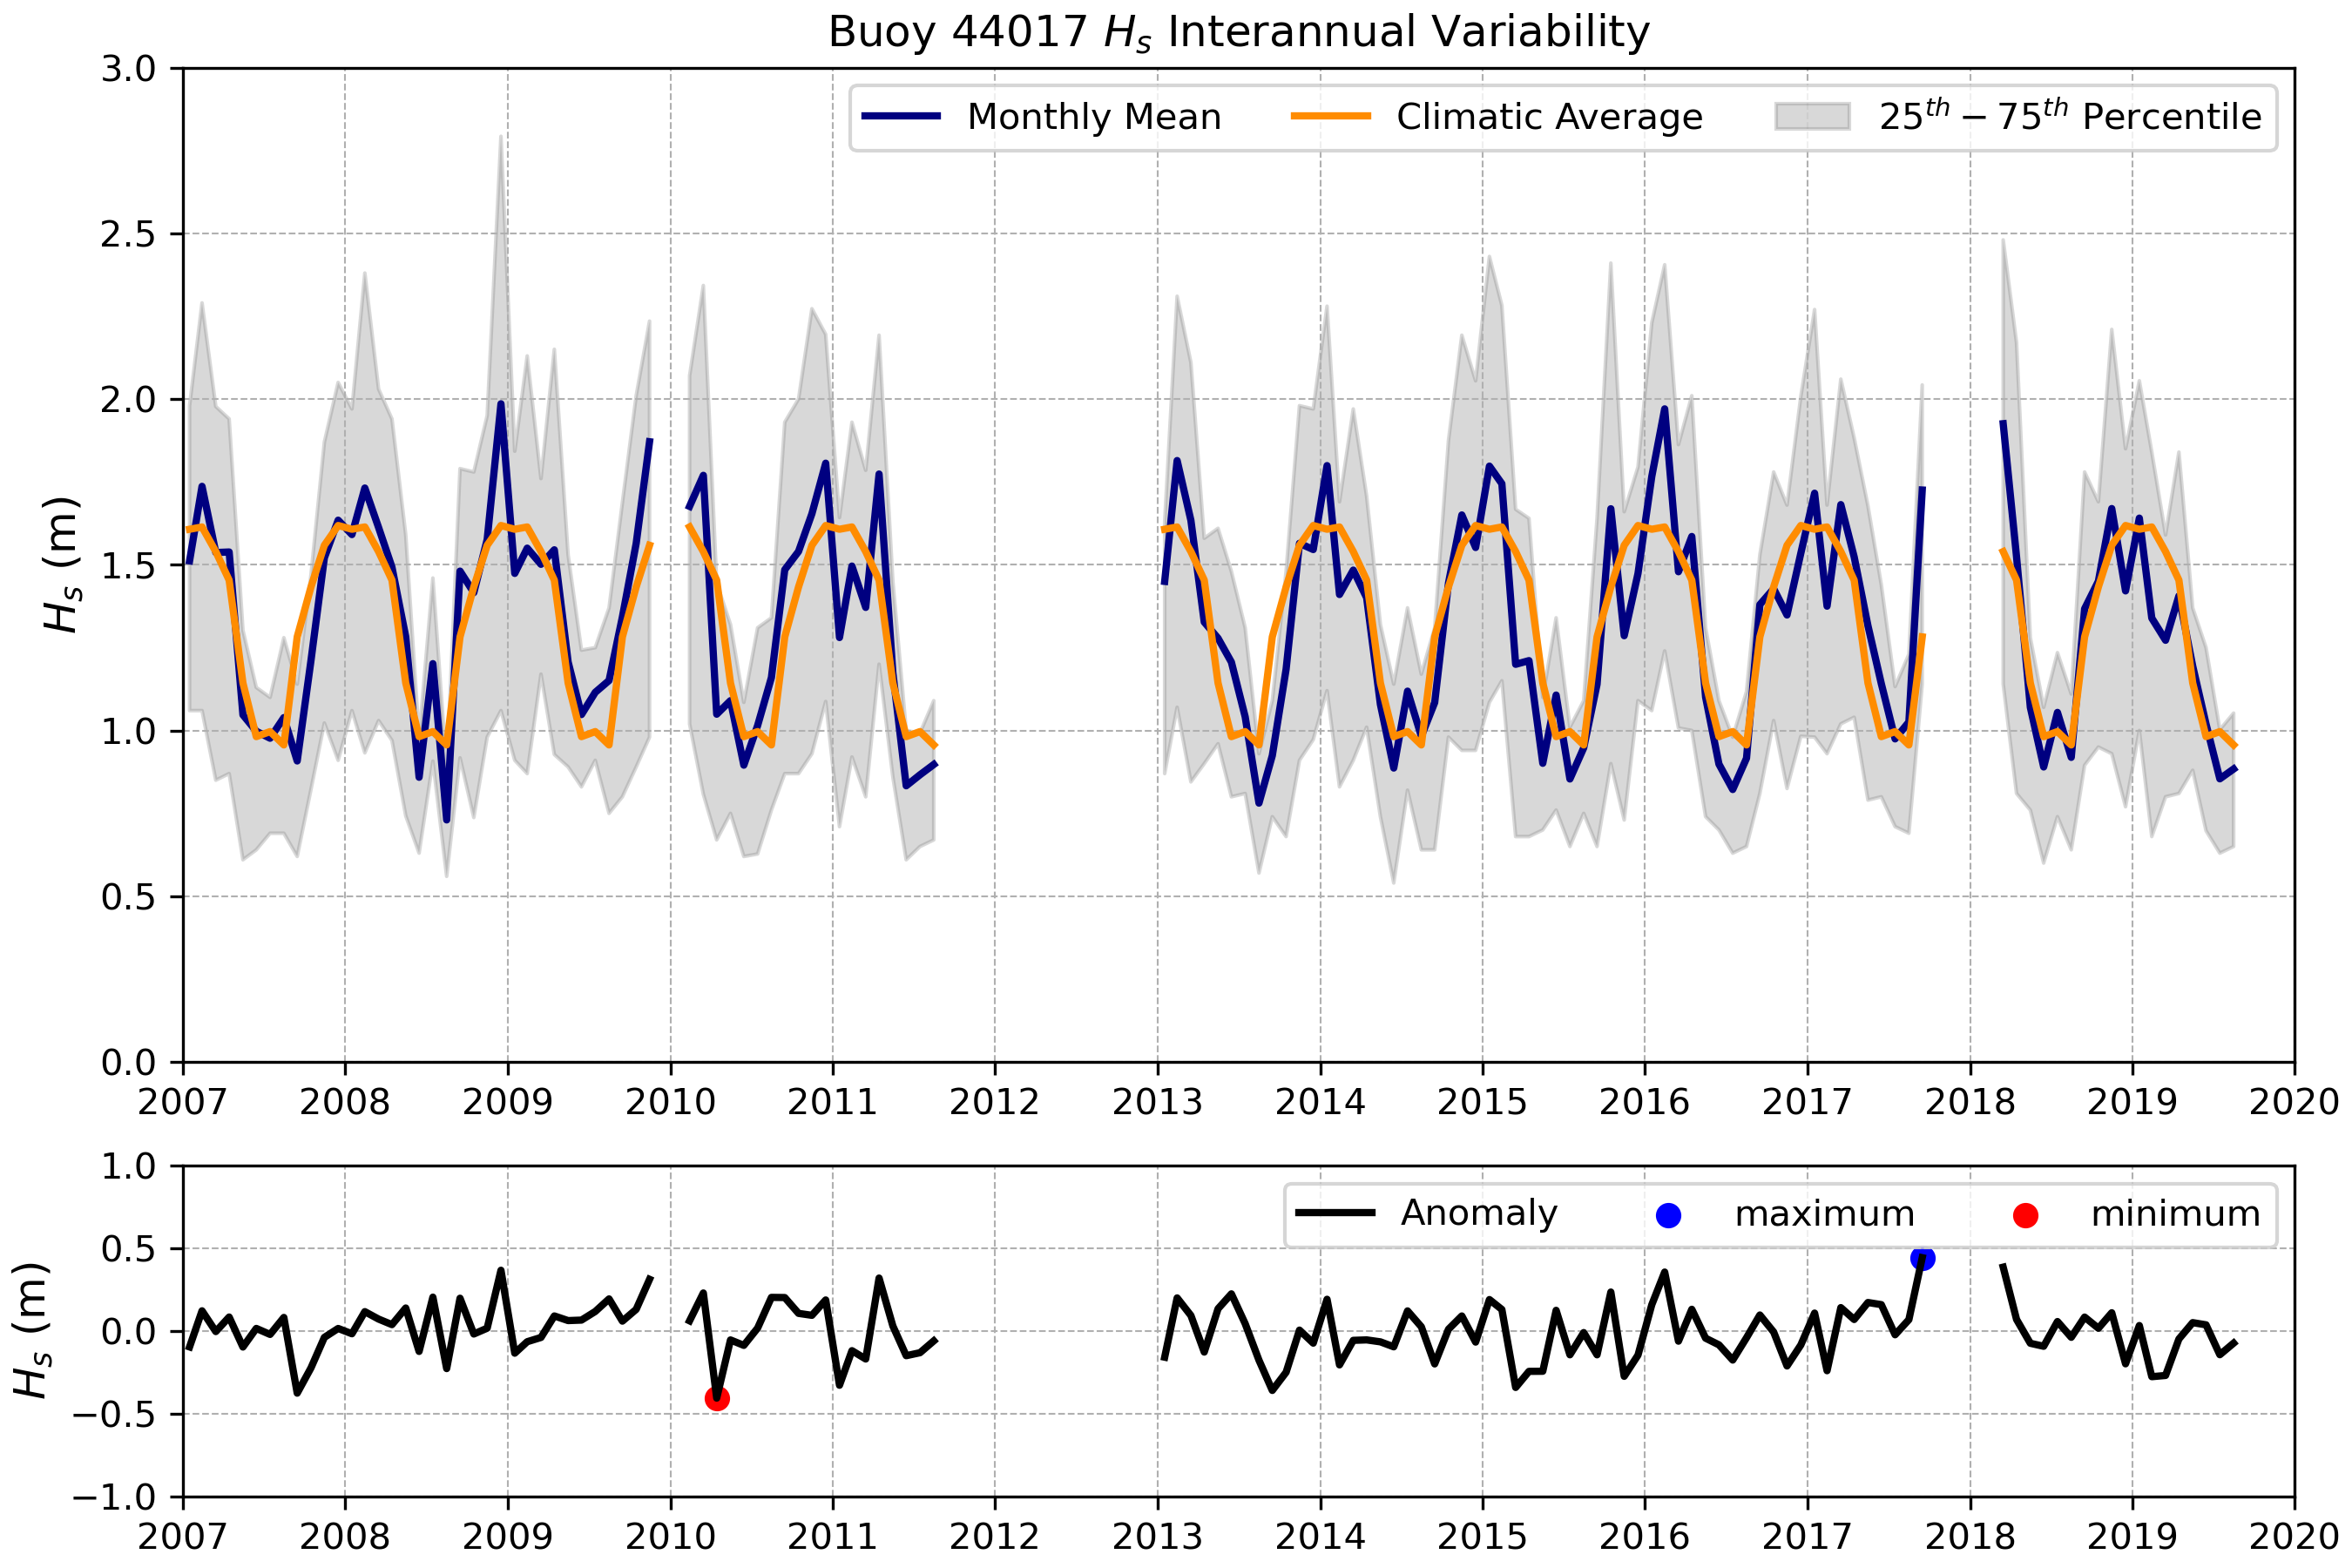
\includegraphics[width=0.83\linewidth]{Figures/Chapter5/b44017_interranual_anomaly_hs.png}
%\decoRule
\caption{Buoy 44017 $u_{10}$ interannual variability including monthly mean values, 25th and 75th percentiles, climatic average and monthly anomalies.}
\label{fig:b44017_wave_inter}
\end{figure}


\begin{figure}[H]
\centering
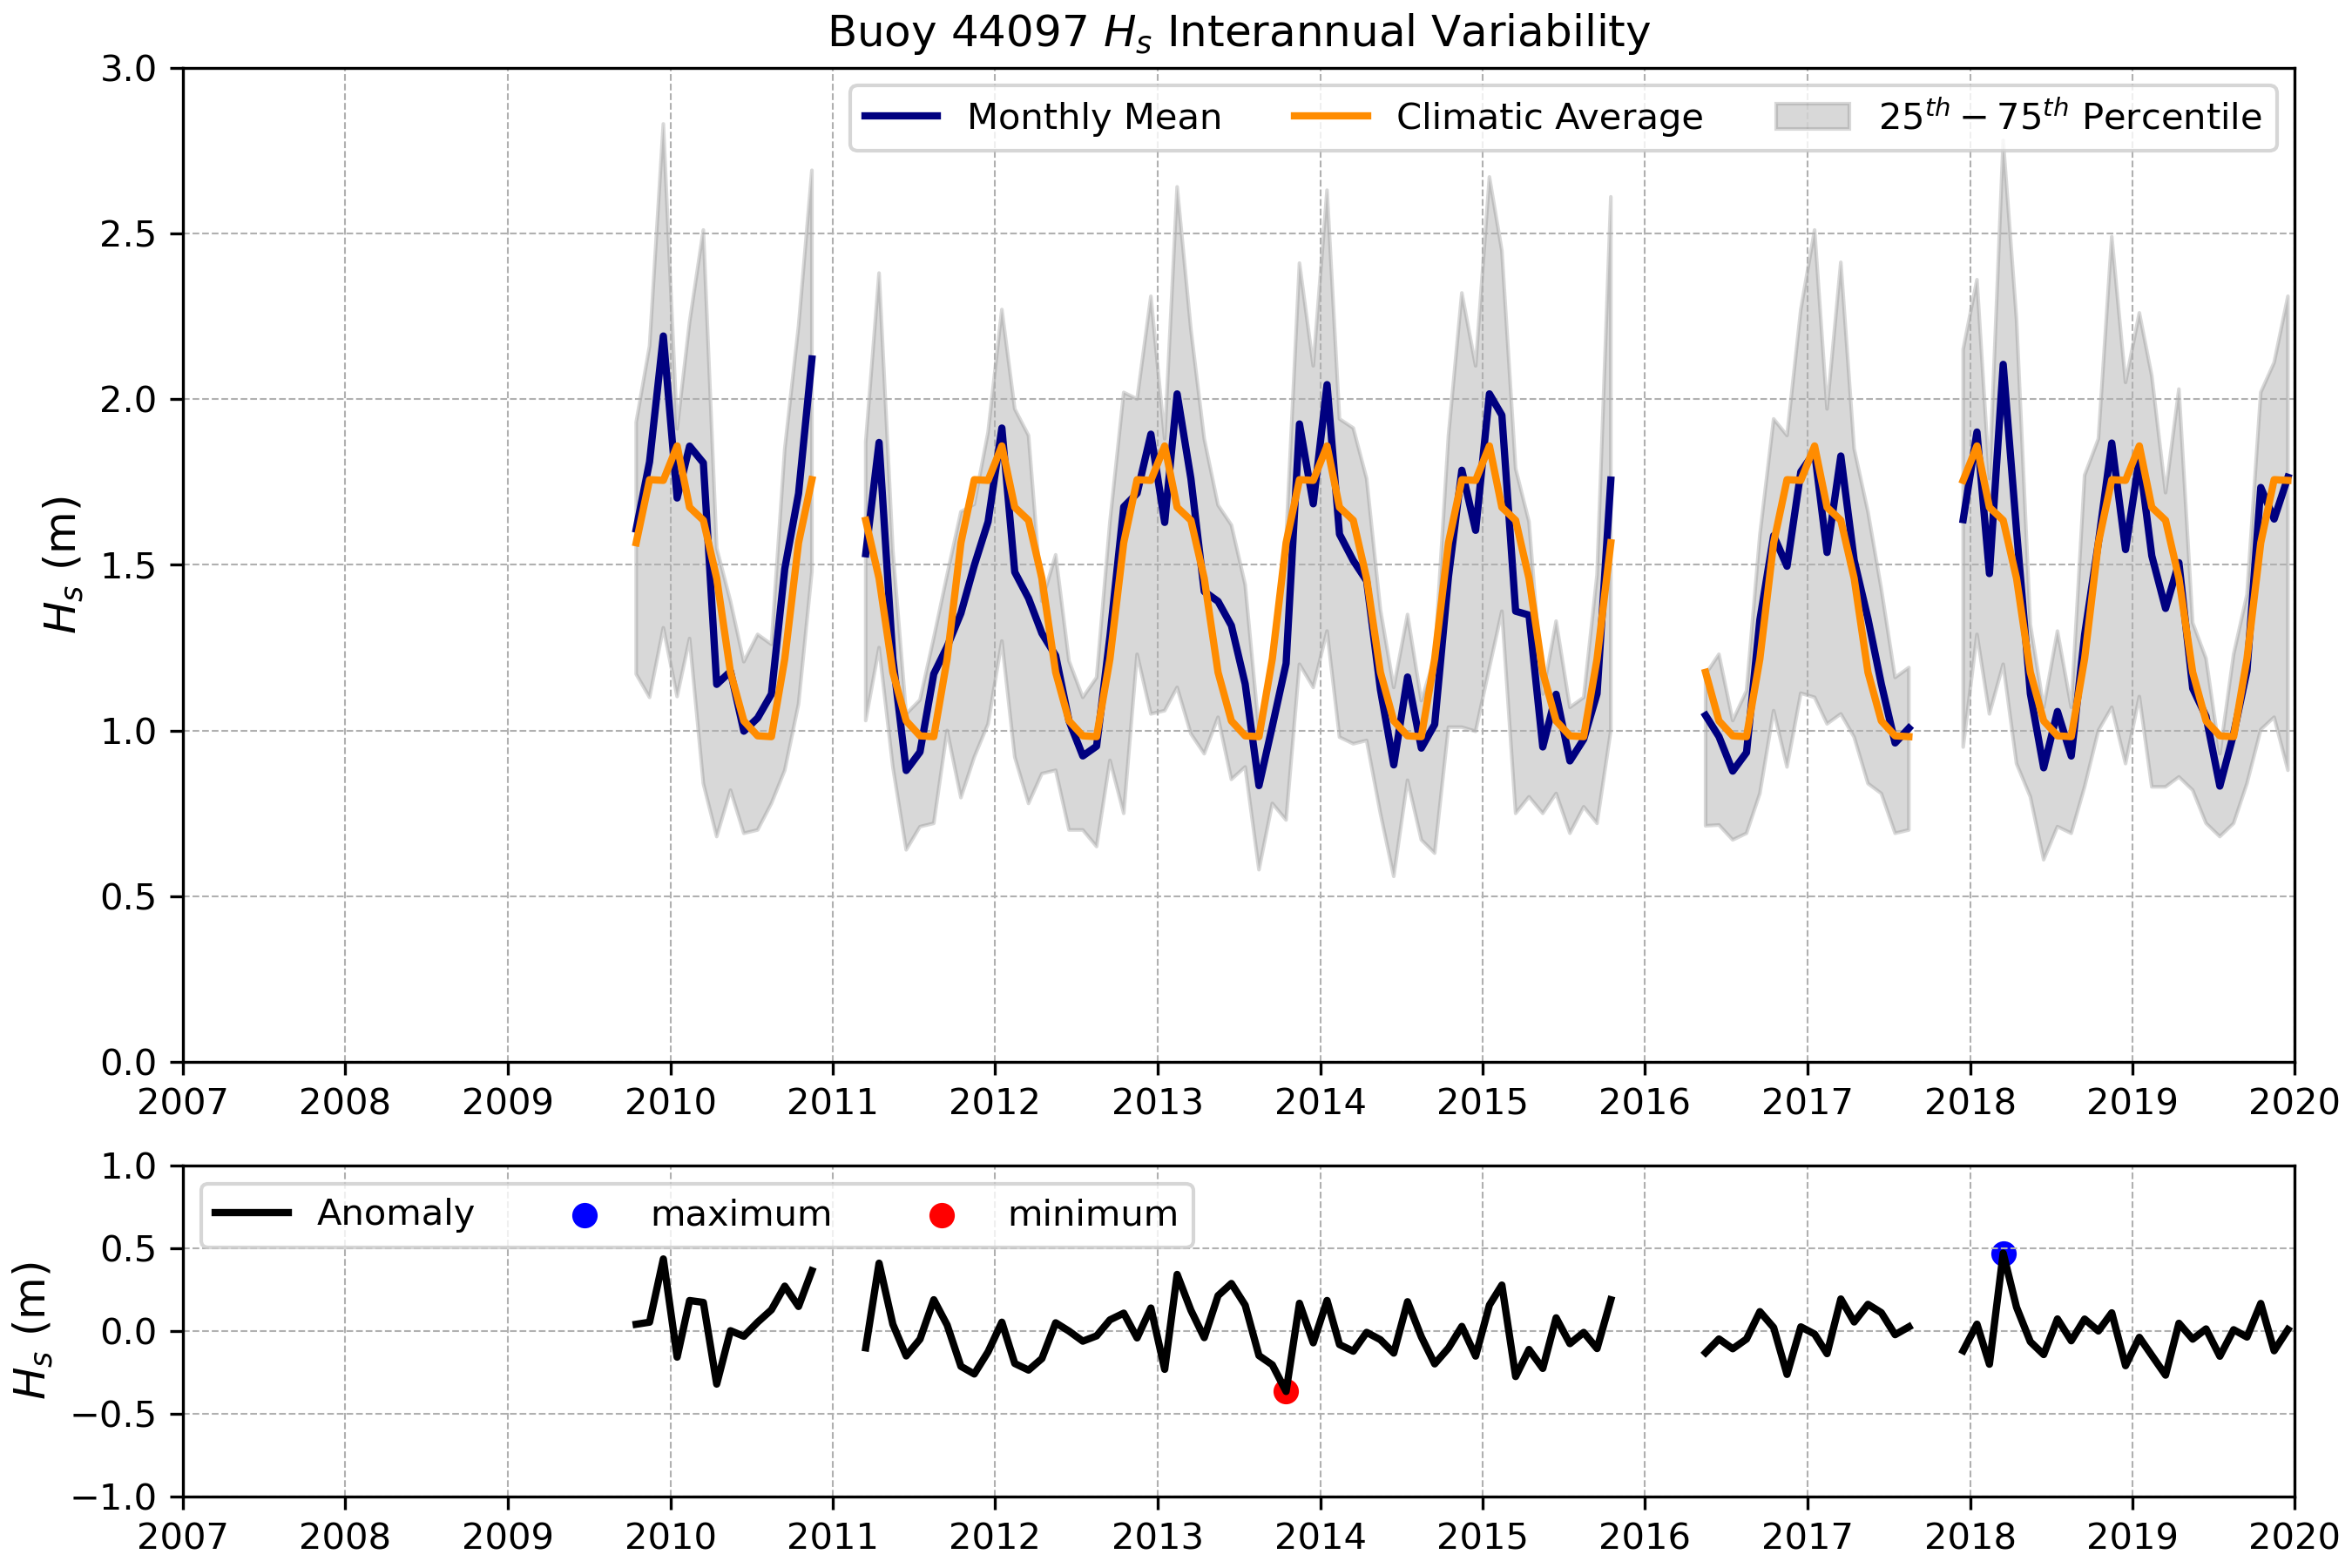
\includegraphics[width=0.83\linewidth]{Figures/Chapter5/b44097_interranual_anomaly_hs.png}
%\decoRule
\caption{Buoy 44097 $u_{10}$ interannual variability including monthly mean values, 25th and 75th percentiles, climatic average and monthly anomalies.}
\label{fig:b44097_wave_inter}
\end{figure}

Specifically, double peaks appear regularly due to the southeastern swell system with the highest energy in March and November combined with the sea states' lower energy density during February and secondarily January.   
However, there are not available wind data for this station for further assessment. Judging from Figure~\ref{fig:b44025_wind_inter}, double peaks exist in the $u_{10}$ winter monthly means. Multiple winter peaks also appear in the corresponding $H_{s}$ Figure~\ref{fig:b44025_wave_inter} for buoy 44025. Finally, the local $H_{s}$ maxima during the summer months described in \ref{seasonal_variability} is also present in the interannual variability figures and the monthly mean time series.


%------------------------------------------------------------------------------------------


\subsection{Wind and Wave Directional Distribution}

The directional distribution of WS and SWH provides us with necessary information on the origin of winds and waves and also their magnitude in each direction. For the WS, the statistical distribution and visualization with a wind rose are adequate to assess the wind direction regime. On the other hand, wave distribution also requires more elaborate analysis due to multiple wave systems present. 

The WS and SWH directional distribution tables and figures include only winter and summer data, and the directional spectra include all available data for the 2007-2019 period. Data from seven buoys were used for the analysis of joint WS and wind direction. Eight buoys record both SWH and mean wave direction data, and they were used for the SWH directional wave distribution. Six buoys are common for wind and wave analysis, buoy 44039 misses wave direction, and the two CDIP buoys (44097 and 44091) do not record wind data. The eight main directions from where the wind and waves are coming from were chosen, each with an angular window of 45 degrees. After grouping the data in these directions, the frequency of occurrence, the $u_{10}$, $H_{s}$ average and standard deviation for each direction separately, and including all of them collectively were calculated. The results are presented in tables \ref{tab:wind_distribution_winter} - \ref{tab:wave_distribution_summer}.

The buoy wind data exhibit homogeneous characteristics during the winter and summer seasons. During winter, over 50\% of the observations reveal a wind direction from the west and northwest. The wind is also strongest from these directions. Buoy 44066, the most remote of all stations and located at the western side of SNE, shows the highest average WS values. The sheltered buoy 44020 reports the lowest wind intensity on average. The standard deviation of the WS is highest from the northeastern direction. During summer, the wind shifts to the south, with over 50\% of observations showing wind direction from the west and southwest for each station. The strongest winds during summer are coming from the northeast, and the standard deviation is also higher for the northeastern winds. Buoy 44020 location is the one with the highest average WS value during summer, and it is expected due to the low seasonal variability, as we previously showed in \ref{seasonal_variability}. The reverse is true for buoy 44008, which has the lowest summer WS average, along with buoy 44039, due to high seasonal variability.

In contrast, the waves are not as coherent with respect to their directional distribution, especially during winter. Three parameters impose challenges to predict and characterize the wave climate during winter; strong winds, more frequent low-pressure systems passing over the region, and swell waves reaching SNE from distant North Atlantic storms. All the above lead to the broader spreading of the sea state to more directions and dictate the further investigation of the wave climate using the directional spectrum. Nevertheless, during winter, the wind's impact is most substantial to waves at the buoy 44020 location, to which they are coming from the west and secondarily from the northwest. There is a small influence of swell waves coming from the east in this location. During summer, waves are more coherent, and their dominant directions for most stations are the south and southeast for approximately 60\% of the observations. The only exception is again buoy 44020, to where swells are coming from the east, and the wind waves follow the direction of the wind coming from the southwest.



\begin{table}[H]
\begin{tabular*}{\textwidth}{c@{\hskip 0.07in}cccccccccc @{\extracolsep{\fill}} cccccccccc}
\toprule
    \textbf{Buoy} & \textbf{Statistics} &  \textbf{N} & \textbf{NE}  & \textbf{E} & \textbf{SE} &  \textbf{S} &  \textbf{SW}  &  \textbf{W}  &  \textbf{NW}  & \textbf{uni}  \\ \midrule
    ~     & Frequency (\%)  & 11.3  & 7.43 & 6.15 & 4.48 & 8.52  & 13.83 & 20.92 & 27.37 & 100  \\
    44025 & Average (m/s)   & 8.08  & 8.05 & 8.24 & 6.84 & 7.6   & 8.02  & 9.86  & 10.43 & 9    \\
    ~     & St. Dev. (m/s)  & 3.79  & 4.57 & 4.08 & 3.78 & 3.6   & 3.37  & 4.08  & 3.92  & 4.08 \\ \midrule
    ~     & Frequency (\%)  & 8.93  & 6.5  & 6.66 & 4.83 & 6.36  & 14.08 & 29.5  & 23.14 & 100  \\
    44017 & Average (m/s)   & 8.1   & 8.81 & 9.19 & 7.29 & 7.87  & 8.54  & 10.17 & 9.56  & 9.18 \\
    ~     & St. Dev. (m/s)  & 4.05  & 4.99 & 4.13 & 3.38 & 3.71  & 3.53  & 3.94  & 3.65  & 3.98 \\ \midrule
    ~     & Frequency (\%)  & 9.6   & 7.67 & 5.24 & 3.28 & 10.25 & 12.9  & 26.03 & 25.02 & 100  \\
    44065 & Average (m/s)   & 7.73  & 8.32 & 7.36 & 5.65 & 7.31  & 6.95  & 9.36  & 9.9   & 8.51 \\
    ~     & St. Dev. (m/s)  & 3.61  & 4.13 & 4.05 & 3.69 & 3.37  & 3.18  & 3.83  & 3.87  & 3.93 \\ \midrule
    ~     & Frequency (\%)  & 11    & 5.41 & 5.81 & 5.13 & 6.85  & 13.03 & 29.95 & 22.83 & 100  \\
    44020 & Average (m/s)   & 8.04  & 8.11 & 8.08 & 6.64 & 6.88  & 7.13  & 8.63  & 9.12  & 8.2  \\
    ~     & St. Dev. (m/s)  & 4.18  & 4.98 & 4.01 & 3.56 & 3.69  & 3.13  & 3.75  & 3.61  & 3.86 \\ \midrule
    ~     & Frequency (\%)  & 11.16 & 6.91 & 6.67 & 6.91 & 8.13  & 13.37 & 21.63 & 25.22 & 100  \\
    44008 & Average (m/s)   & 8.9   & 8.16 & 8.13 & 7.49 & 7.92  & 8.48  & 10.1  & 9.94  & 9.09 \\
    ~     & St. Dev. (m/s)  & 4.47  & 4.74 & 3.84 & 3.61 & 3.74  & 3.87  & 4.36  & 4.01  & 4.22 \\ \midrule
    ~     & Frequency (\%)  & 13.95 & 6.09 & 8.67 & 3.78 & 6.43  & 11.29 & 26.57 & 23.23 & 100  \\
    44039 & Average (m/s)   & 6.82  & 6.47 & 7.22 & 5.5  & 5.31  & 6.24  & 8.32  & 8.39  & 7.38 \\
    ~     & St. Dev. (m/s)  & 3.2   & 3.4  & 3.8  & 3.48 & 3.37  & 3.07  & 3.59  & 3.34  & 3.57 \\ \midrule
    ~     & Frequency (\%)  & 10.77 & 7.24 & 5.35 & 4.81 & 7.34  & 13.94 & 22.47 & 28.07 & 100  \\
    44066 & Average (m/s)   & 8.45  & 8.85 & 8.41 & 7.89 & 8.01  & 9.23  & 10.52 & 10.34 & 9.52 \\
    ~     & St. Dev. (m/s)  & 4.22  & 4.98 & 4.36 & 3.98 & 3.80  & 3.79  & 4.04  & 3.74  & 4.13 \\ \bottomrule
\end{tabular*}
\caption {Directional Distribution of winter $u_{10}$ frequency, average and standard deviation using buoy data.}
\label{tab:wind_distribution_winter}
\end{table}

\begin{figure}[H]
\centering
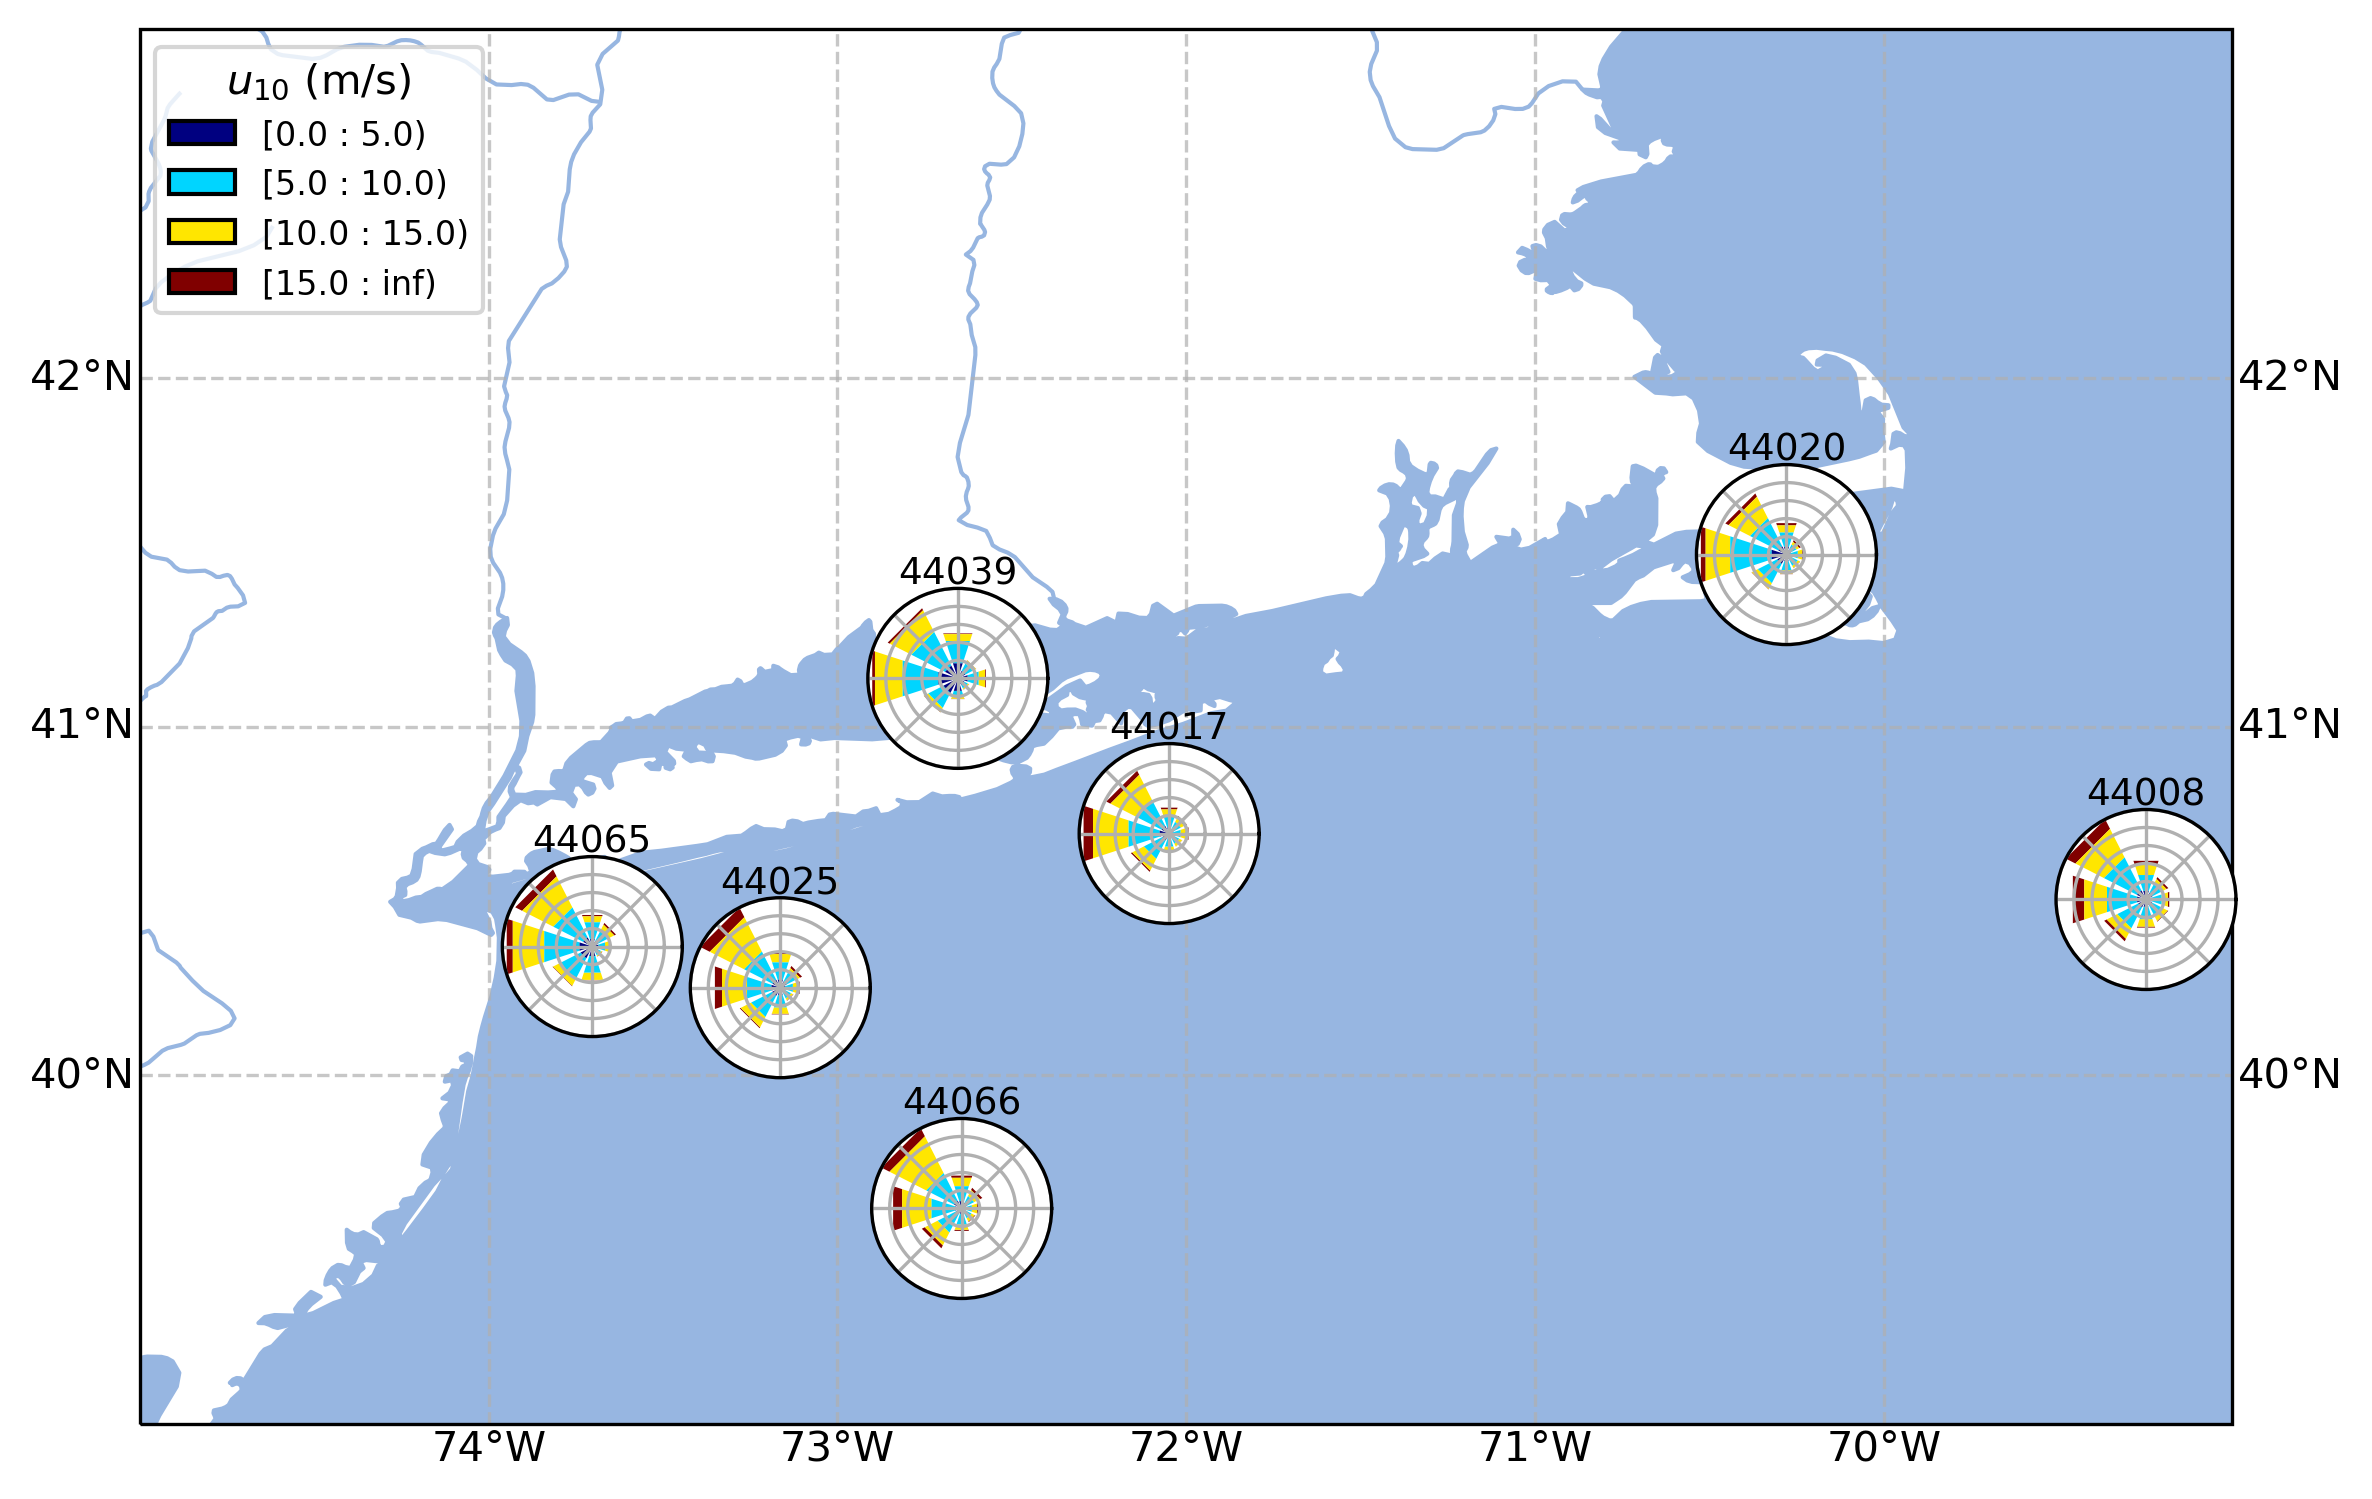
\includegraphics[width=0.81\linewidth]{Figures/Chapter5/windrose_map_winter1.png}
%\decoRule
\caption{Buoy wind rose map for the winter season.}
\label{fig:windrose_map_winter}
\end{figure}




\begin{table}[H]
\begin{tabular*}{\textwidth}{c@{\hskip 0.07in}cccccccccc @{\extracolsep{\fill}} cccccccccc}
\toprule
    \textbf{Buoy} & \textbf{Statistics} &  \textbf{N} & \textbf{NE}  & \textbf{E} & \textbf{SE} &  \textbf{S} &  \textbf{SW}  &  \textbf{W}  &  \textbf{NW}  & \textbf{uni}  \\ \midrule
    ~       & Frequency (\%)  & 6.22 & 8.42  & 9.32  & 8.08  & 19.95 & 29.6  & 11.03 & 7.38 & 100  \\
    44025   & Average (m/s)   & 5.3  & 6.25  & 5.6   & 4.54  & 5.62  & 5.93  & 4.81  & 5.22 & 5.54 \\
    ~       & St. Dev. (m/s)  & 2.82 & 3.19  & 2.85  & 2.3   & 2.38  & 2.41  & 2.15  & 3.84 & 2.6  \\ \midrule
    ~       & Frequency (\%)  & 5.11 & 7.27  & 7.67  & 7.36  & 14.28 & 37.35 & 13.57 & 7.39 & 100  \\
    44017   & Average (m/s)   & 5.42 & 6.97  & 6.26  & 4.7   & 4.88  & 5.9   & 4.83  & 5.12 & 5.54 \\
    ~       & St. Dev. (m/s)  & 2.88 & 3.69  & 3.19  & 2.51  & 2.31  & 2.29  & 2.17  & 2.68 & 2.64 \\ \midrule
    ~       & Frequency (\%)  & 6.02 & 6.7   & 8.63  & 8.21  & 28.54 & 19.46 & 13.34 & 9.09 & 100  \\
    44065   & Average (m/s)   & 5.21 & 5.98  & 5.77  & 4.6   & 6.04  & 4.96  & 4.55  & 5.41 & 5.38 \\
    ~       & St. Dev. (m/s)  & 2.71 & 3.03  & 2.8   & 2.24  & 2.49  & 2.14  & 2.12  & 2.71 & 2.53 \\ \midrule
    ~       & Frequency (\%)  & 7.22 & 9.22  & 8.77  & 7.11  & 15.68 & 35.88 & 10.63 & 5.49 & 100  \\
    44020   & Average (m/s)   & 5.86 & 6.16  & 5.05  & 5.22  & 6.3   & 6.68  & 5.62  & 5.87 & 6.11 \\
    ~       & St. Dev. (m/s)  & 3    & 2.92  & 2,67  & 2.94  & 2.84  & 2.41  & 2.7   & 2.99 & 2.76 \\ \midrule
    ~       & Frequency (\%)  & 8.37 & 10.81 & 8.49  & 10.16 & 21.02 & 23.05 & 10.67 & 7.44 & 100  \\
    44008   & Average (m/s)   & 4.93 & 5.6   & 4.71  & 4.31  & 4.62  & 4.77  & 4.29  & 4.61 & 4.73 \\
    ~       & St. Dev. (m/s)  & 2.82 & 2.98  & 2.69  & 2.34  & 2.24  & 2.14  & 2.15  & 2.63 & 2.46 \\ \midrule
    ~       & Frequency (\%)  & 8.14 & 5.98  & 12.35 & 6.77  & 18.45 & 22.91 & 17.35 & 8.05 & 100  \\
    44039   & Average (m/s)   & 4.57 & 4.87  & 5.22  & 4.39  & 4.7   & 4.74  & 4.37  & 4.62 & 4.69 \\
    ~       & St. Dev. (m/s)  & 2.34 & 2.68  & 2.74  & 2.43  & 2.2   & 2.07  & 2.1   & 2.45 & 2.32 \\ \midrule
    ~       & Frequency (\%)  & 7.18 & 9.79  & 8.63  & 7.5   & 16.63 & 29.8  & 12.74 & 7.76 & 100  \\
    44066   & Average (m/s)   & 6.05 & 6.55  & 5.55  & 4.9   & 5.51  & 6.24  & 5.02  & 5.16 & 5.74 \\
    ~       & St. Dev. (m/s)  & 3.34 & 3.21  & 3.06  & 2.58  & 2.46  & 2.47  & 2.34  & 2.81 & 2.75 \\ \bottomrule
\end{tabular*}
\caption {Directional Distribution of summer $u_{10}$ frequency, average and standard deviation using buoy data.}
\label{tab:wind_distribution_summer}
\end{table}


\begin{figure}[H]
\centering
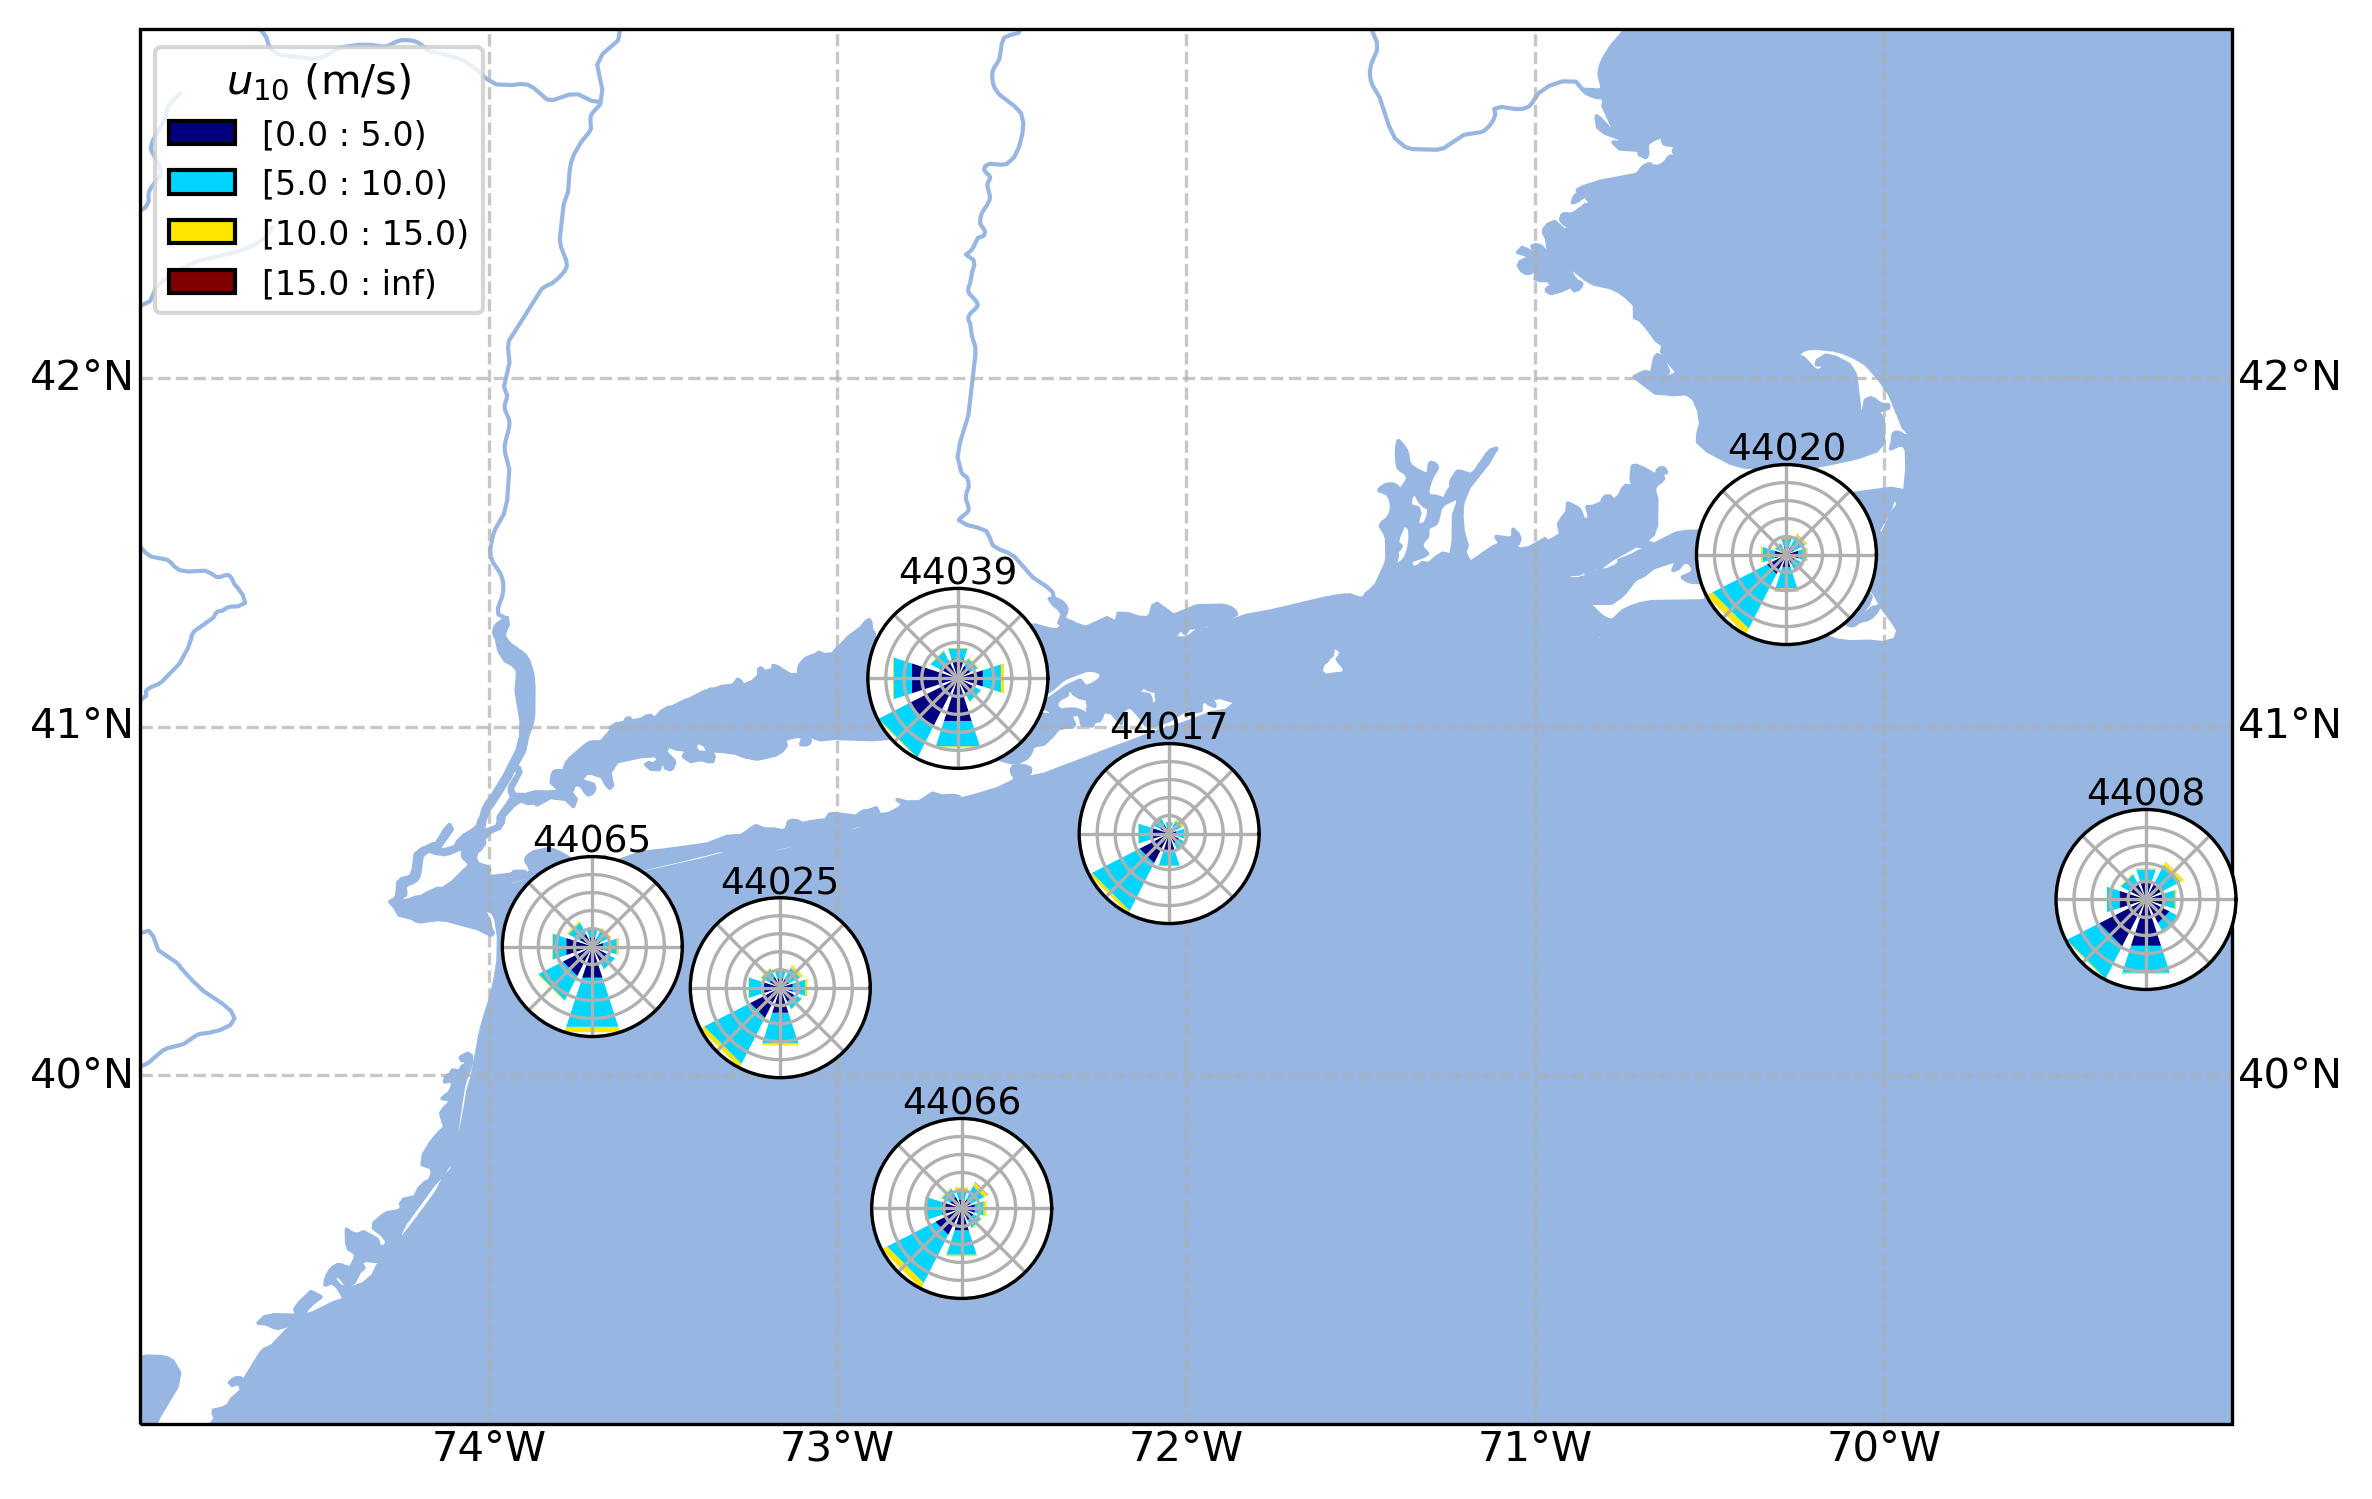
\includegraphics[width=0.81\linewidth]{Figures/Chapter5/windrose_map_summer1.png}
%\decoRule
\caption{Buoy wind rose map for the summer season.}
\label{fig:windrose_map_summer}
\end{figure}


\begin{table}[H]
\begin{tabular*}{\textwidth}{c@{\hskip 0.07in}cccccccccc @{\extracolsep{\fill}} cccccccccc}
\toprule
    \textbf{Buoy} & \textbf{Statistics} &  \textbf{N} & \textbf{NE}  & \textbf{E} & \textbf{SE} &  \textbf{S} &  \textbf{SW}  &  \textbf{W}  &  \textbf{NW}  & \textbf{uni}  \\ \midrule
    ~     & Frequency (\%)  & 2.41  & 3.08 & 16.54 & 20.97 & 18.67 & 7.03  & 22.83 & 8.45  & 100  \\
    44025 & Average (m)   & 1.24  & 1.24 & 1.59  & 1.42  & 1.53  & 1.33  & 1.65  & 1.46  & 1.51 \\
    ~     & St. Dev. (m)  & 0.77  & 0.85 & 1.04  & 0.94  & 0.76  & 0.66  & 0.71  & 0.67  & 0.84 \\ \midrule
    ~     & Frequency (\%)  & 1.95  & 3.56 & 14.44 & 22.09 & 22.84 & 24.56 & 5.87  & 4.7   & 100  \\
    44017 & Average (m)   & 1.09  & 1.4  & 1.65  & 1.57  & 1.79  & 1.66  & 1.36  & 1.3   & 1.61 \\
    ~     & St. Dev. (m)  & 0.48  & 0.81 & 0.98  & 1     & 0.88  & 0.77  & 0.68  & 0.54  & 0.88 \\ \midrule
    ~     & Frequency (\%)  & 1.82  & 0.84 & 18.88 & 30.98 & 20.35 & 1.79  & 7.9   & 17.45 & 100  \\
    44065 & Average (m)   & 0.88  & 0.81 & 1.28  & 1.11  & 1.1   & 0.8   & 1.13  & 1.07  & 1.12 \\
    ~     & St. Dev. (m)  & 0.5   & 0.47 & 0.81  & 0.68  & 0.54  & 0.43  & 0.48  & 0.43  & 0.63 \\ \midrule
    ~     & Frequency (\%)  & 6.81  & 6.74 & 20.71 & 4.3   & 4.69  & 6.23  & 37.23 & 13.29 & 100  \\
    44020 & Average (m)   & 0.78  & 0.86 & 0.57  & 0.63  & 0.61  & 0.56  & 0.72  & 0.76  & 0.69 \\
    ~     & St. Dev. (m)  & 0.46  & 0.57 & 0.33  & 0.36  & 0.31  & 0.24  & 0.32  & 0.38  & 0.37 \\ \midrule
    ~     & Frequency (\%)  & 7.01  & 9.5  & 12.98 & 9.5   & 19.25 & 19.14 & 16.29 & 6.34  & 100  \\
    44008 & Average (m)   & 2.13  & 2.36 & 2.11  & 1.88  & 2.65  & 2.46  & 2.5   & 2.46  & 2.37 \\
    ~     & St. Dev. (m)  & 1.18  & 1.49 & 1.23  & 1.18  & 1.39  & 1.18  & 1.15  & 1.28  & 1.28 \\ \midrule
    ~     & Frequency (\%)  & 4.99  & 3.18 & 4.5   & 18.76 & 22.31 & 21.05 & 17.16 & 8.05  & 100  \\
    44097 & Average (m)   & 1.46  & 1.73 & 1.73  & 1.46  & 1.83  & 1.99  & 1.87  & 1.69  & 1.76 \\
    ~     & St. Dev. (m)  & 0.76  & 0.94 & 0.93  & 0.88  & 1.06  & 1.01  & 0.82  & 0.72  & 0.95 \\ \midrule
    ~     & Frequency (\%)  & 11.23 & 4.2  & 27.32 & 20.78 & 20.14 & 4.88  & 5.01  & 6.44  & 100  \\
    44091 & Average (m)   & 1.29  & 1.63 & 1.52  & 1.24  & 1.45  & 1.18  & 1.43  & 1.43  & 1.4  \\
    ~     & St. Dev. (m)  & 0.56  & 1.02 & 1.01  & 0.65  & 0.61  & 0.47  & 0.51  & 0.54  & 0.76 \\ \midrule
    ~     & Frequency (\%)  & 5.37  & 5.88 & 18.17 & 13.37 & 17.21 & 8.08  & 11.45 & 20.48 & 100  \\
    44066 & Average (m)   & 1.62  & 2.57 & 1.75  & 1.55  & 2     & 1.97  & 2.23  & 2.05  & 1.94 \\
    ~     & St. Dev. (m)  & 0.99  & 1.79 & 1.06  & 1     & 1.06  & 0.9   & 1.06  & 0.99  & 1.11 \\ \bottomrule
\end{tabular*}
\caption {Directional Distribution of winter $H_{s}$ frequency, average and standard deviation for NDBC Buoys and Stations}
\label{tab:wave_distribution_winter}
\end{table}


\begin{figure}[H]
\centering
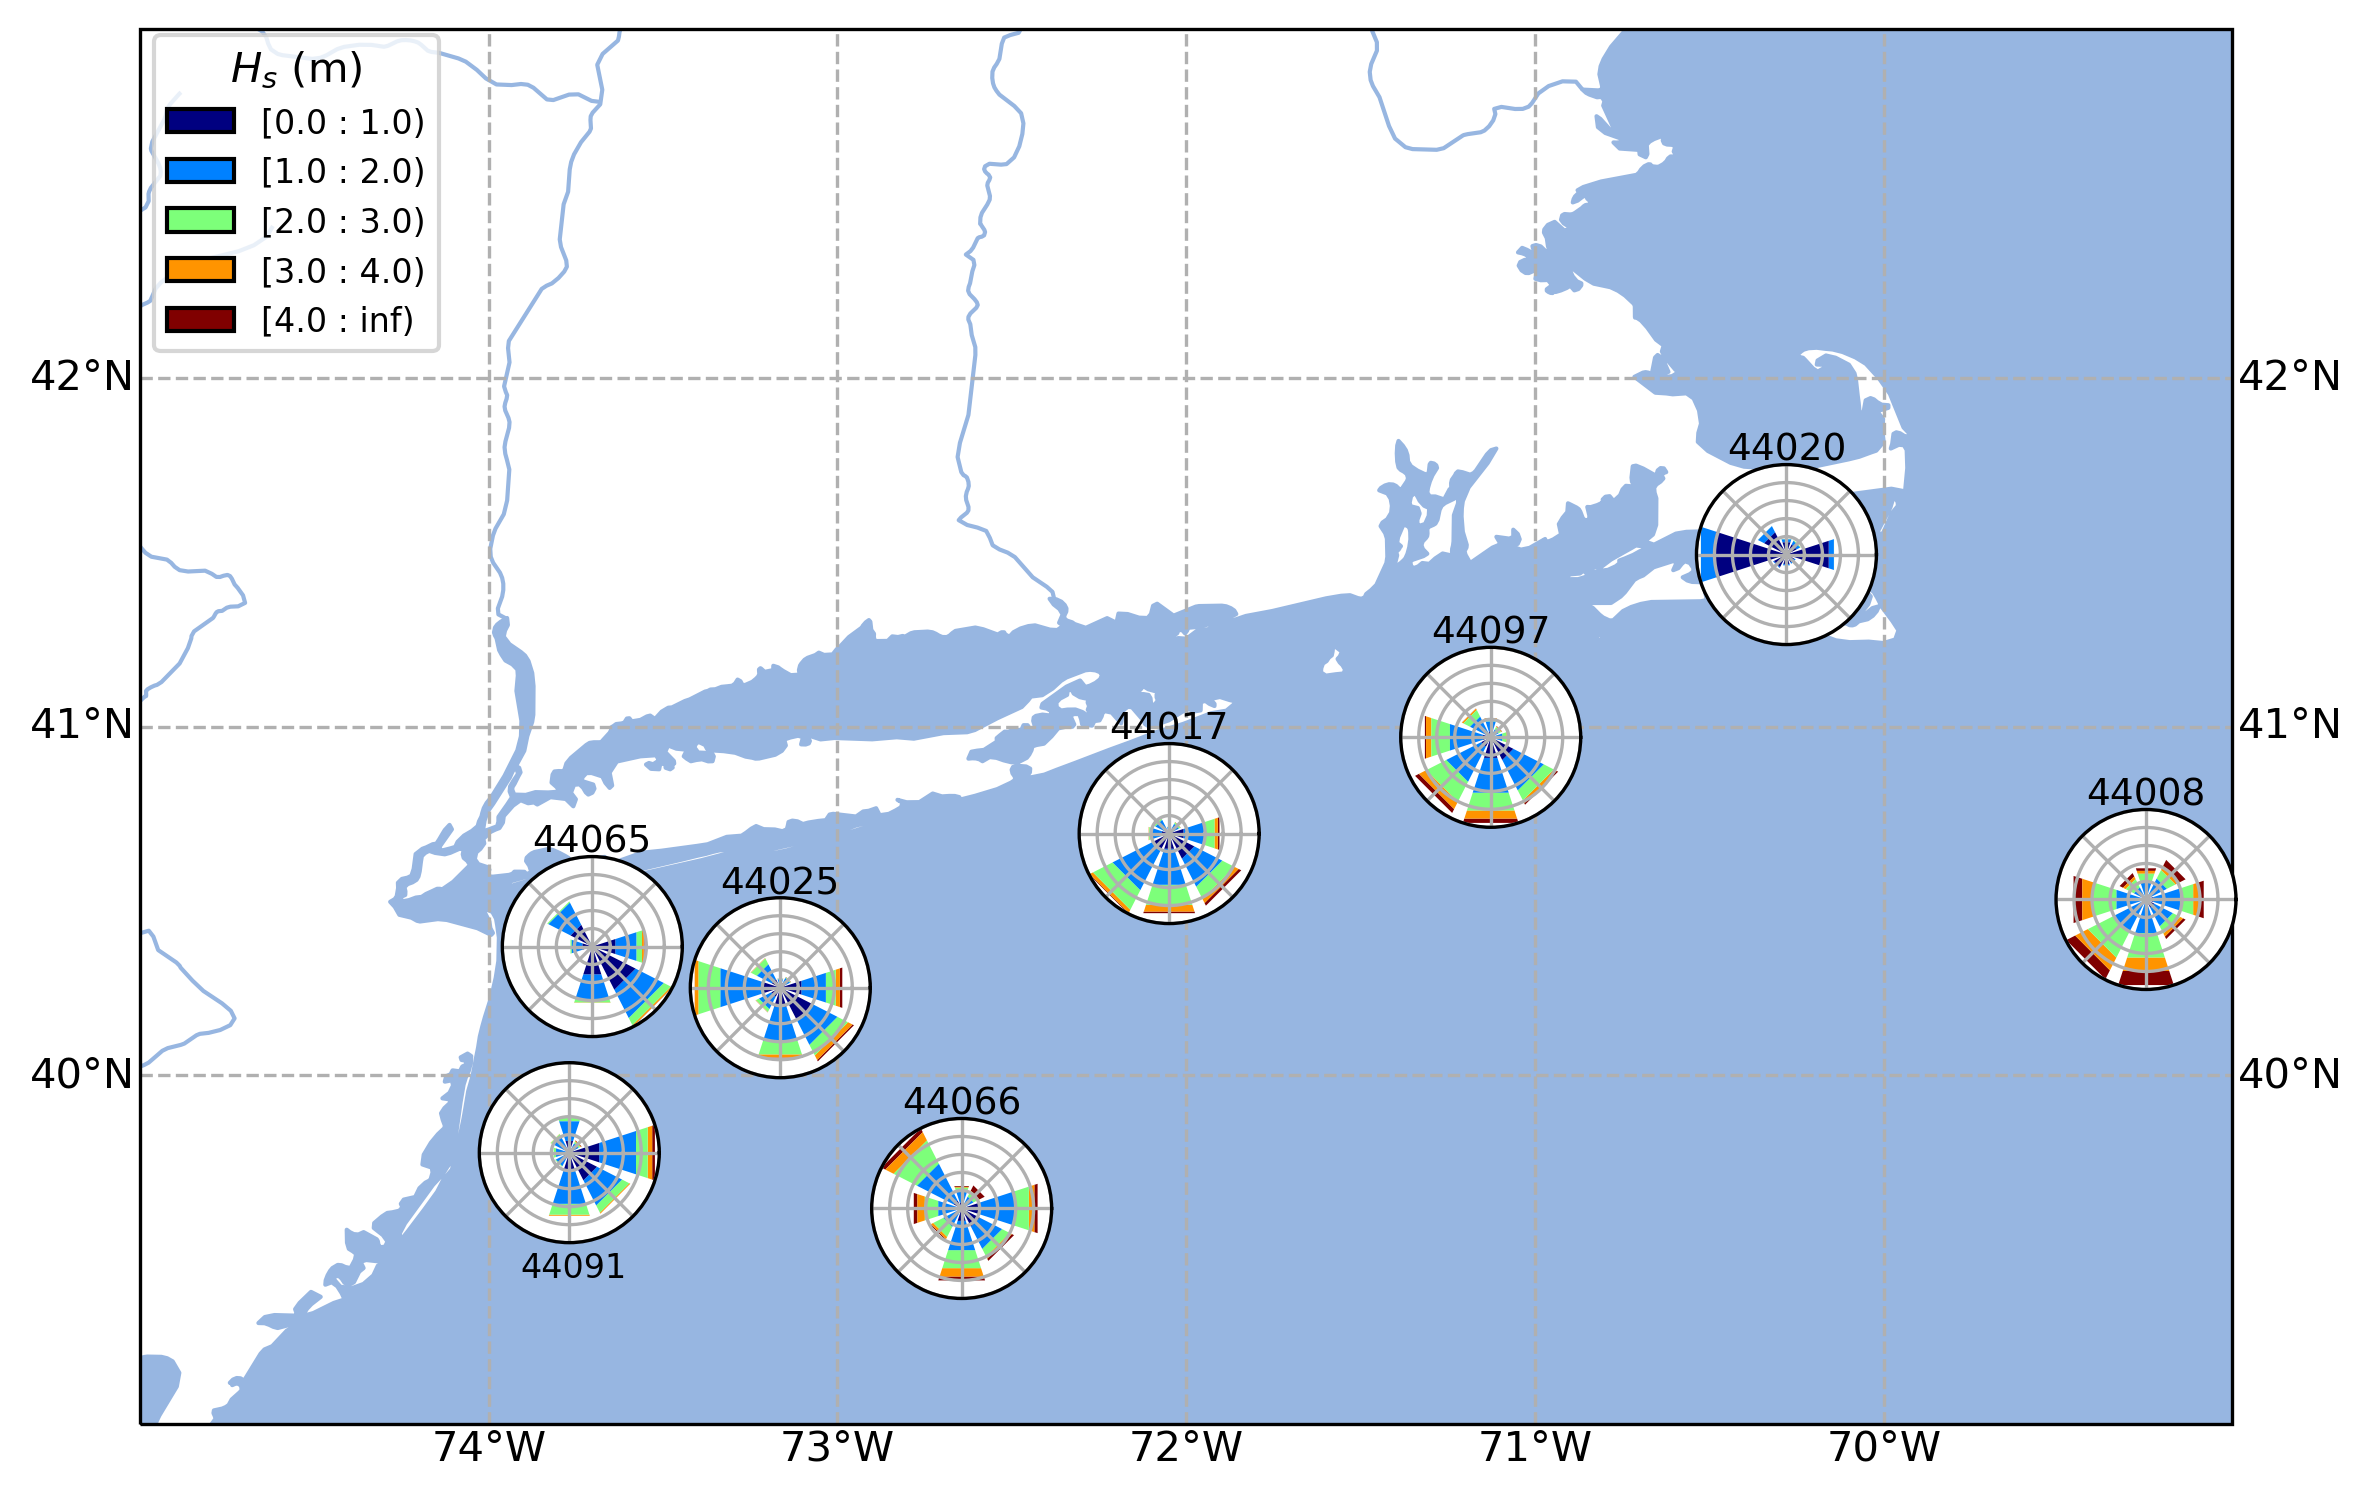
\includegraphics[width=0.81\linewidth]{Figures/Chapter5/waverose_map_winter.png}
%\decoRule
\caption{Winter wave rose map for NDBC buoys}
\label{fig:waverose_map_winter}
\end{figure}



\begin{table}[H]
\begin{tabular*}{\textwidth}{c@{\hskip 0.07in}cccccccccc @{\extracolsep{\fill}} cccccccccc}
\toprule
    \textbf{Buoy} & \textbf{Statistics} &  \textbf{N} & \textbf{NE}  & \textbf{E} & \textbf{SE} &  \textbf{S} &  \textbf{SW}  &  \textbf{W}  &  \textbf{NW}  & \textbf{uni}  \\ \midrule
    ~     & Frequency (\%)  & 0.59 & 1.84 & 16.35 & 34.47 & 37.19 & 7.25  & 1.62  & 0.69 & 100  \\
    44025 & Average (m)   & 0.93 & 1.1  & 1.05  & 0.87  & 1.02  & 0.99  & 0.89  & 0.88 & 0.97 \\
    ~     & St. Dev. (m)  & 0.26 & 0.42 & 0.52  & 0.4   & 0.38  & 0.35  & 0.29  & 0.29 & 0.41 \\ \midrule
    ~     & Frequency (\%)  & 0.31 & 1.88 & 12.65 & 32.94 & 39.49 & 11.9  & 0.57  & 0.27 & 100  \\
    44017 & Average (m)   & 0.87 & 1.23 & 0.98  & 0.9   & 1.05  & 0.99  & 0.77  & 0.88 & 0.99 \\
    ~     & St. Dev. (m)  & 0.31 & 0.46 & 0.43  & 0.42  & 0.43  & 0.34  & 0.24  & 0.23 & 0.42 \\ \midrule
    ~     & Frequency (\%)  & 0.3  & 0.48 & 15.23 & 43.98 & 37.35 & 1.17  & 0.27  & 1.22 & 100  \\
    44065 & Average (m)   & 0.75 & 0.72 & 0.91  & 0.78  & 0.87  & 0.82  & 0.73  & 0.75 & 0.83 \\
    ~     & St. Dev. (m)  & 0.18 & 0.26 & 0.41  & 0.34  & 0.34  & 0.36  & 0.39  & 0.21 & 0.36 \\ \midrule
    ~     & Frequency (\%)  & 7.91 & 9.4  & 20.32 & 8.05  & 11.11 & 18.31 & 17.81 & 7.08 & 100  \\
    44020 & Average (m)   & 0.44 & 0.56 & 0.4   & 0.44  & 0.47  & 0.46  & 0.46  & 0.43 & 0.45 \\
    ~     & St. Dev. (m)  & 0.21 & 0.3  & 0.18  & 0.23  & 0.19  & 0.16  & 0.16  & 0.18 & 0.2  \\ \midrule
    ~     & Frequency (\%)  & 1.37 & 4.54 & 17.93 & 24.02 & 34.62 & 14.45 & 2.78  & 0.29 & 100  \\
    44008 & Average (m)   & 1.23 & 1.35 & 1.08  & 0.97  & 1.21  & 1.25  & 1.06  & 1.1  & 1.14 \\
    ~     & St. Dev. (m)  & 0.43 & 0.62 & 0.5   & 0.45  & 0.53  & 0.6   & 0.35  & 0.4  & 0.53 \\ \midrule
    ~     & Frequency (\%)  & 0.57 & 1.51 & 2.57  & 28    & 38.6  & 23.88 & 4.23  & 0.64 & 100  \\
    44097 & Average (m)   & 1.09 & 1.19 & 1.17  & 0.86  & 0.98  & 1.16  & 1.01  & 0.96 & 1    \\
    ~     & St. Dev. (m)  & 0.33 & 0.3  & 0.51  & 0.38  & 0.39  & 0.53  & 0.35  & 0.29 & 0.44 \\ \midrule
    ~     & Frequency (\%)  & 1.78 & 1.78 & 26.02 & 29.97 & 36.51 & 3.16  & 0.13  & 0.65 & 100  \\
    44091 & Average (m)   & 0.97 & 1.35 & 1.05  & 0.88  & 1.01  & 0.91  & 1.07  & 0.97 & 0.99 \\
    ~     & St. Dev. (m)  & 0.56 & 1.02 & 1.01  & 0.65  & 0.61  & 0.47  & 0.51  & 0.54 & 0.76 \\ \midrule
    ~     & Frequency (\%)  & 1.07 & 3.18 & 17.81 & 27.61 & 31.59 & 14.79 & 1.66  & 2.29 & 100  \\
    44066 & Average (m)   & 1.08 & 1.44 & 1.12  & 0.84  & 1.13  & 1.11  & 1     & 1.21 & 1.05 \\
    ~     & St. Dev. (m)  & 0.32 & 0.56 & 0.49  & 0.37  & 0.35  & 0.26  & 0.39  & 0.28 & 0.4  \\ \bottomrule
\end{tabular*}
\caption {Directional Distribution of summer $H_{s}$ frequency, average and standard deviation for NDBC Buoys and Stations}
\label{tab:wave_distribution_summer}
\end{table}


\begin{figure}[H]
\centering
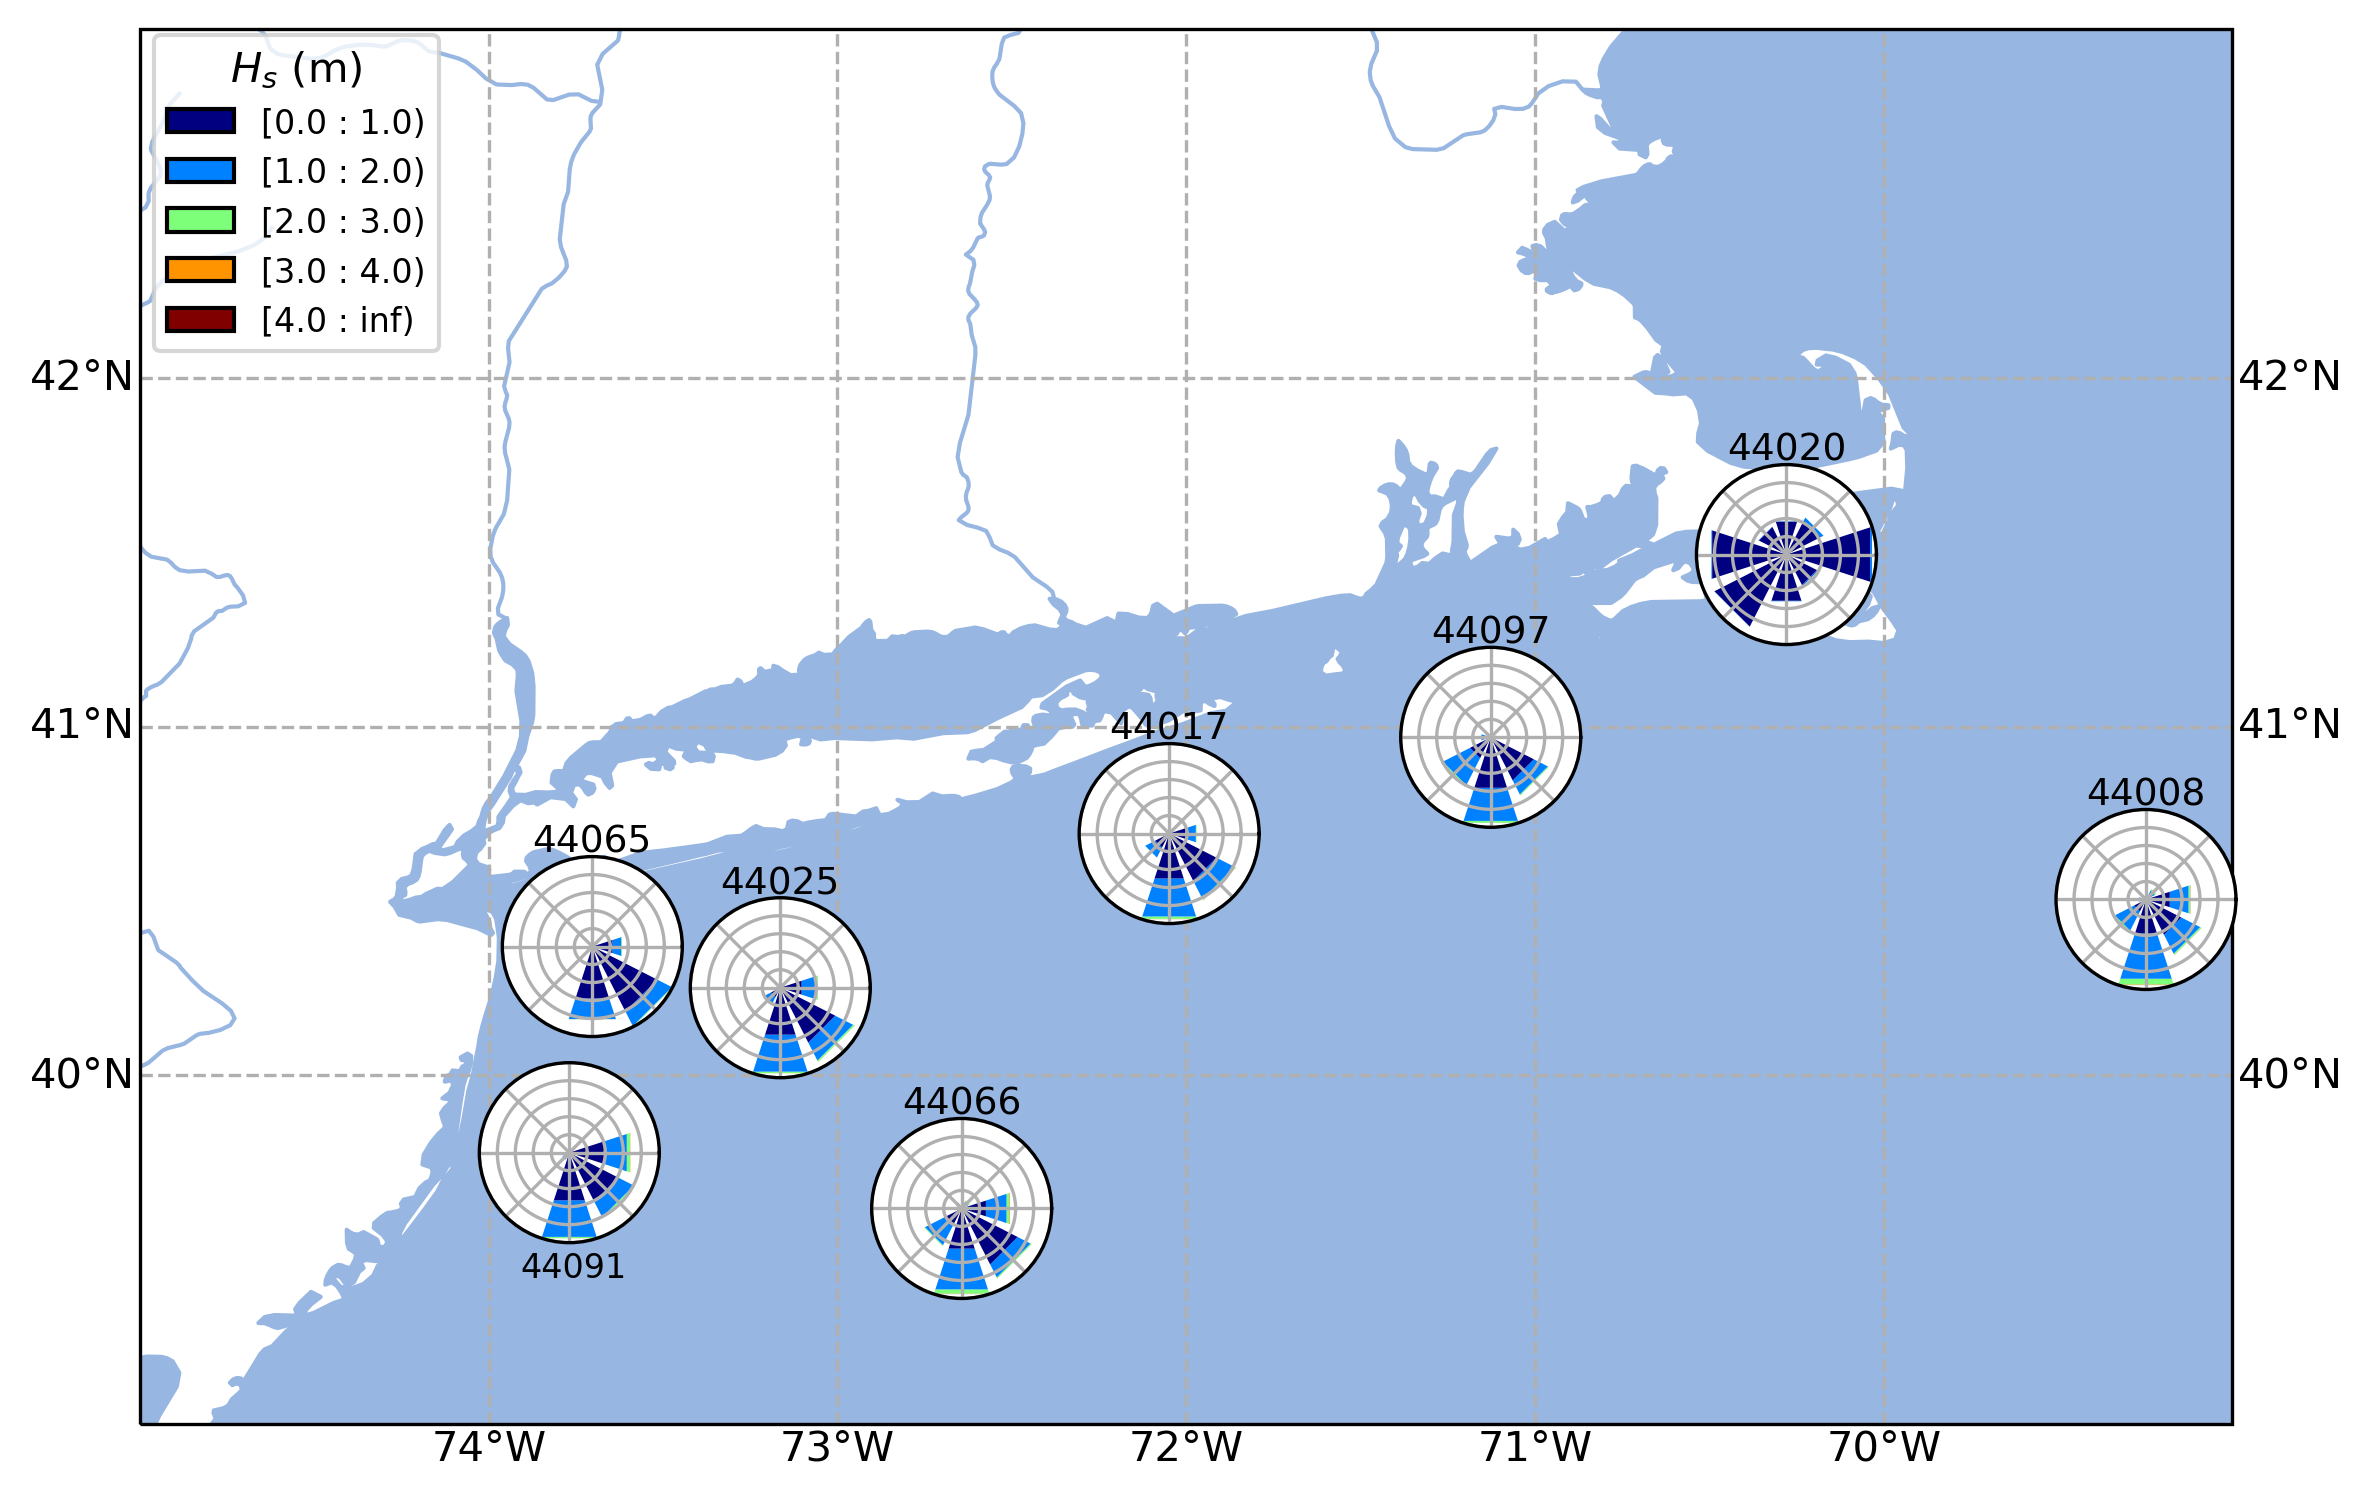
\includegraphics[width=0.81\linewidth]{Figures/Chapter5/waverose_map_summer.png}
%\decoRule
\caption{Summer wave rose map for NDBC buoys and Stations}
\label{fig:waverose_map_summer}
\end{figure}


 

The wave directional spectra reveal even more detailed characteristics of the wave climate. Specifically, Figure~\ref{fig:monthly_dir_spectra} shows the buoy 44097 monthly average wave elevation variance density, or energy density as it is commonly referenced, for all direction and frequency bands. This station's selection was made because it is located inside the SNE offshore wind projected area and our main domain of interest.


 \begin{figure}[H]
\centering
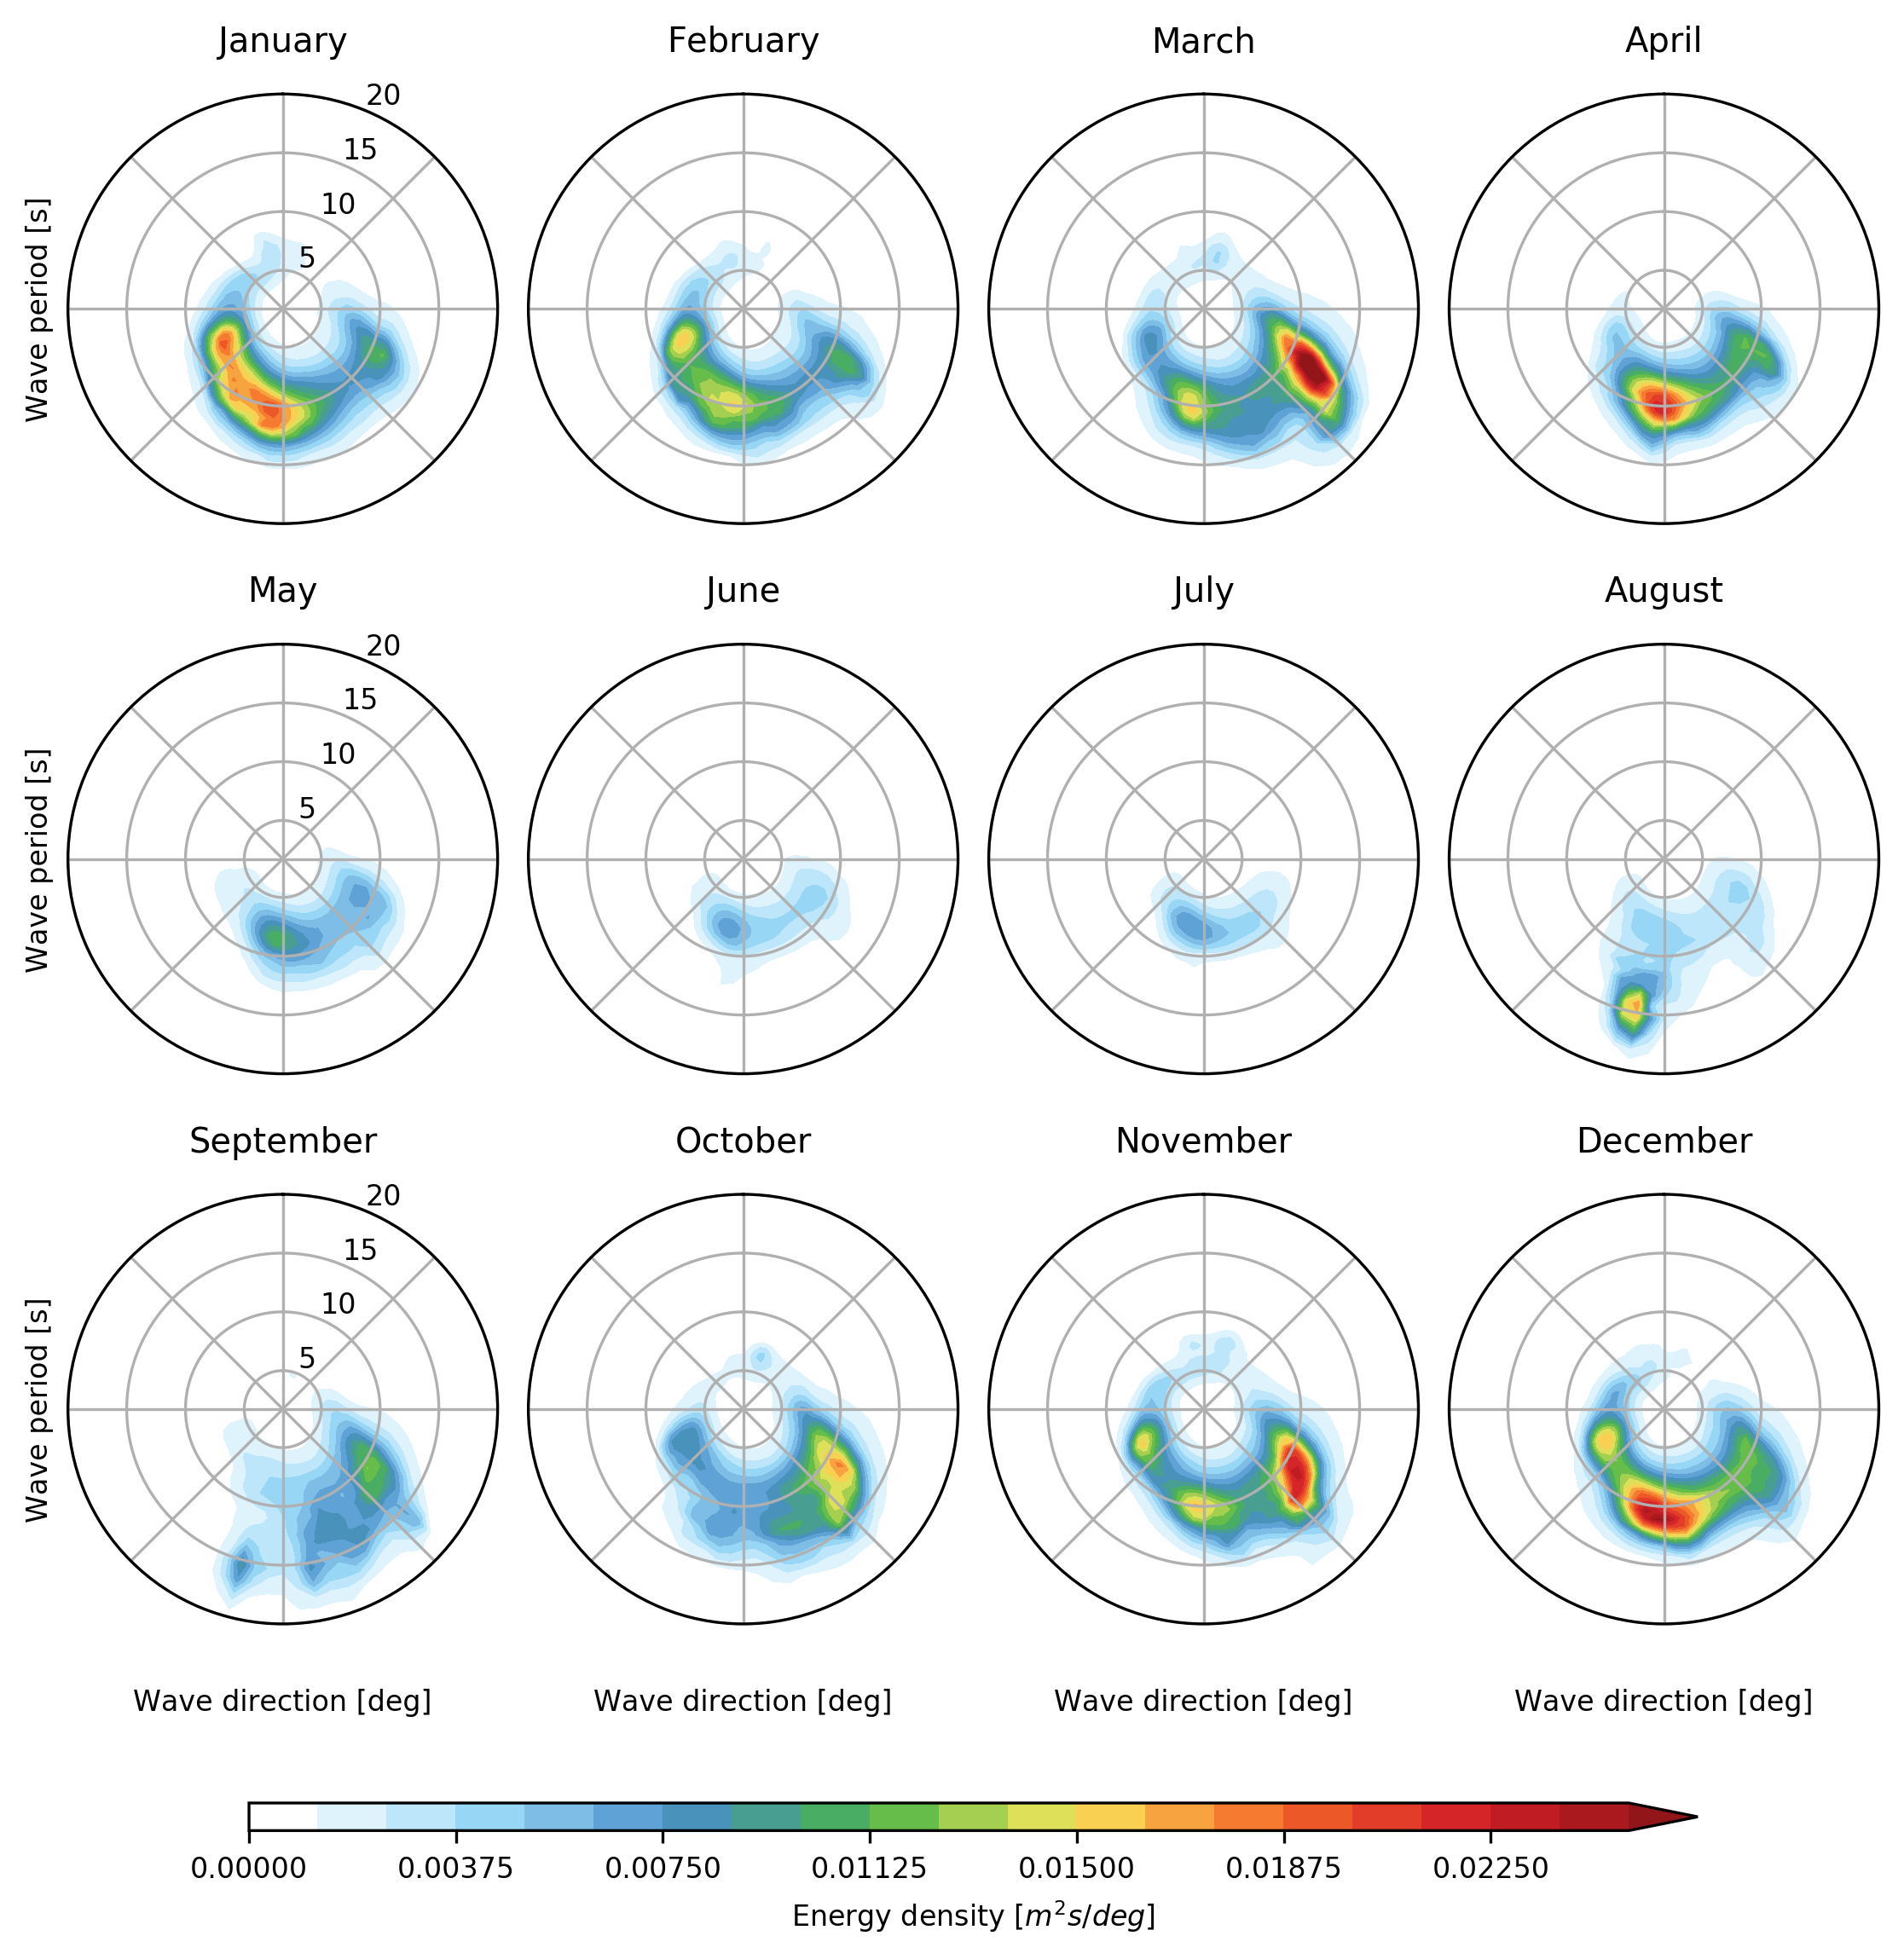
\includegraphics[width=0.95\linewidth]{Figures/Chapter5/monthly_dir_spectra.png}
%\decoRule
\caption{Buoy 44097 monthly average wave variance (energy) density for the 2009-2019 period.}
\label{fig:monthly_dir_spectra}
\end{figure}


Three main wave systems can be identified with distinct directions, periods, and development of their variance density throughout the year. The first one is a wind wave system, judging from its direction and range of periods. This wave system propagates its energy from the southwest with average periods of between 6 to 8 seconds, and it is evolving from October to April, with a peak in January. Starting from May and during the summer months, this system shifts its direction to southern with noticeably lower energy. The second system is a mixed swell-wind wave system that propagates from the south. It is evolving from November until April with maximum variance density in December and April. The third one is a swell system with a 10 to 15 seconds period range propagating from the southeast. This system is strongest in March and November, but it shows considerable energy from September to April. Besides, all three main systems are present from November until March with distinct levels of variance density. Finally, the southern wave direction during summer, evident in Figure~\ref{fig:waverose_map_summer}, is caused mainly by the southern swell with the highest energy density during August, with periods close to 15 seconds.




\section{Wind Speed Probability Density Functions}


The process of fitting to the theoretical probability functions and the estimation of the corresponding parameters was described in \ref{wind_wave_pdfs}. The initial assessment and comparison between the \emph{SciPy} extended library of PDFs is not included in this section. Only the estimated parameters, statistics, and figures of the four best fitted PDFs to each boy's data are included. The evaluation of the fitting is performed with the Kolmogorov-Smirnov (K-S) goodness-of-fit test and the calculation of the K-S error, which represents the deviation of the empirical Cumulative Distribution Function (CDF) to the theoretical. The distribution with the smallest K-S error value is often proposed as the best fit. For further assessment, the probability plots for each buoy and each of the four proposed PDFs are also added, including the coefficient of determination ($R^{2}$). 

All calculations were performed to WS data from four selected buoys with a distance less than 50 kilometers from the coast. First, a table including the estimated PDF parameters are presented for each buoy's time series and all four distributions. The four distributions included are the ones with the smallest K-S error among the 90 distributions available in the \emph{SciPy} library. Finally, Figure \ref{fig:pdfs_wind} contains all empirical PDFs that fit best to the buoys' data and also the $u_{10}$ histograms.

Based on the K-S error values in Table~\ref{tab:wind_pdfs} and the coefficients of determination on the probability plots, the distributions that best fit the data are the Beta and Johnson $S_{B}$ for the coastal buoys 44025, 44017, and 44065, which are located between 20 and 40 kilometers off the coast. For the sheltered buoy 44020, the Weibull 3P distribution is accepted as the best to describe the long-term $u_{10}$ distribution.


\begin{table}[H]
\centering
\begin{tabular*}{0.85\textwidth}{c@{\hskip 0.25in}ccccccc @{\extracolsep{\fill}} ccccccc}
\toprule
   Buoy & PDF &  shape $\alpha$ &  shape $\beta$ &  location $\gamma$ &   scale $\eta$  & K-S error \\
\midrule
 \multirow{4}{*}{44025} &   Johnson $S_{B}$ &  1.45889 &  1.51276 &  -1.36785 &  29.55943 &    0.00855 \\
&         Beta &  2.70274 &  7.88593 &  -0.23496 &  29.49847 &    0.00861 \\
 &   Weibull 3P &  2.02042 &        - &   0.01575 &   8.21624 &    0.01256 \\
 &     Rayleigh &       2 &        - &   0.04085 &   5.78170 &    0.01034 \\ \midrule
 \multirow{4}{*}{44017} &   Johnson $S_{B}$ &  1.26469 &  1.39953 &  -1.02751 &  27.13660 &    0.00870 \\
 &         Beta &  2.50125 &  6.73867 &  -0.08808 &  27.31905 &    0.00892 \\
 &   Weibull 3P &   2.00142 &        - &   0.05729 &   8.18246 &    0.01318 \\
 &     Rayleigh &      2 &        - &   0.05897 &   5.78394 &    0.01301 \\ \midrule
\multirow{4}{*}{44065} &   Johnson $S_{B}$ &  1.45918 &  1.52591 &  -1.34807 &  28.62410 &    0.01001 \\
  &         Beta &  2.70918 &  7.70465 &  -0.21269 &  28.02316 &    0.00808 \\
  &   Weibull 3P &  2.03604	 &        - &   0.02152 &   7.96683 &    0.01285 \\
 &     Rayleigh &       2 &        - &   0.06330 &   5.58648 &    0.01106 \\ \midrule
\multirow{4}{*}{44020} &   Johnson $S_{B}$ &  1.69612 &  1.78309 &  -2.17746 &  32.48900 &    0.01429 \\
&         Beta &  3.44047 &  10.4444 &  -0.64746 &  32.00931 &    0.01364 \\
&   Weibull 3P &   2.16096 &        - &  -0.04203 &   8.27184 &    0.01086 \\
 &     Rayleigh &       2 &        - &   0.12833 &   5.65487 &    0.03053 \\
\bottomrule
\end{tabular*}
\caption {$u_{10}$ Probability Density Function parameter and K-S error statistics.}
\label{tab:wind_pdfs}
\end{table}





\begin{figure}[H]
\centering
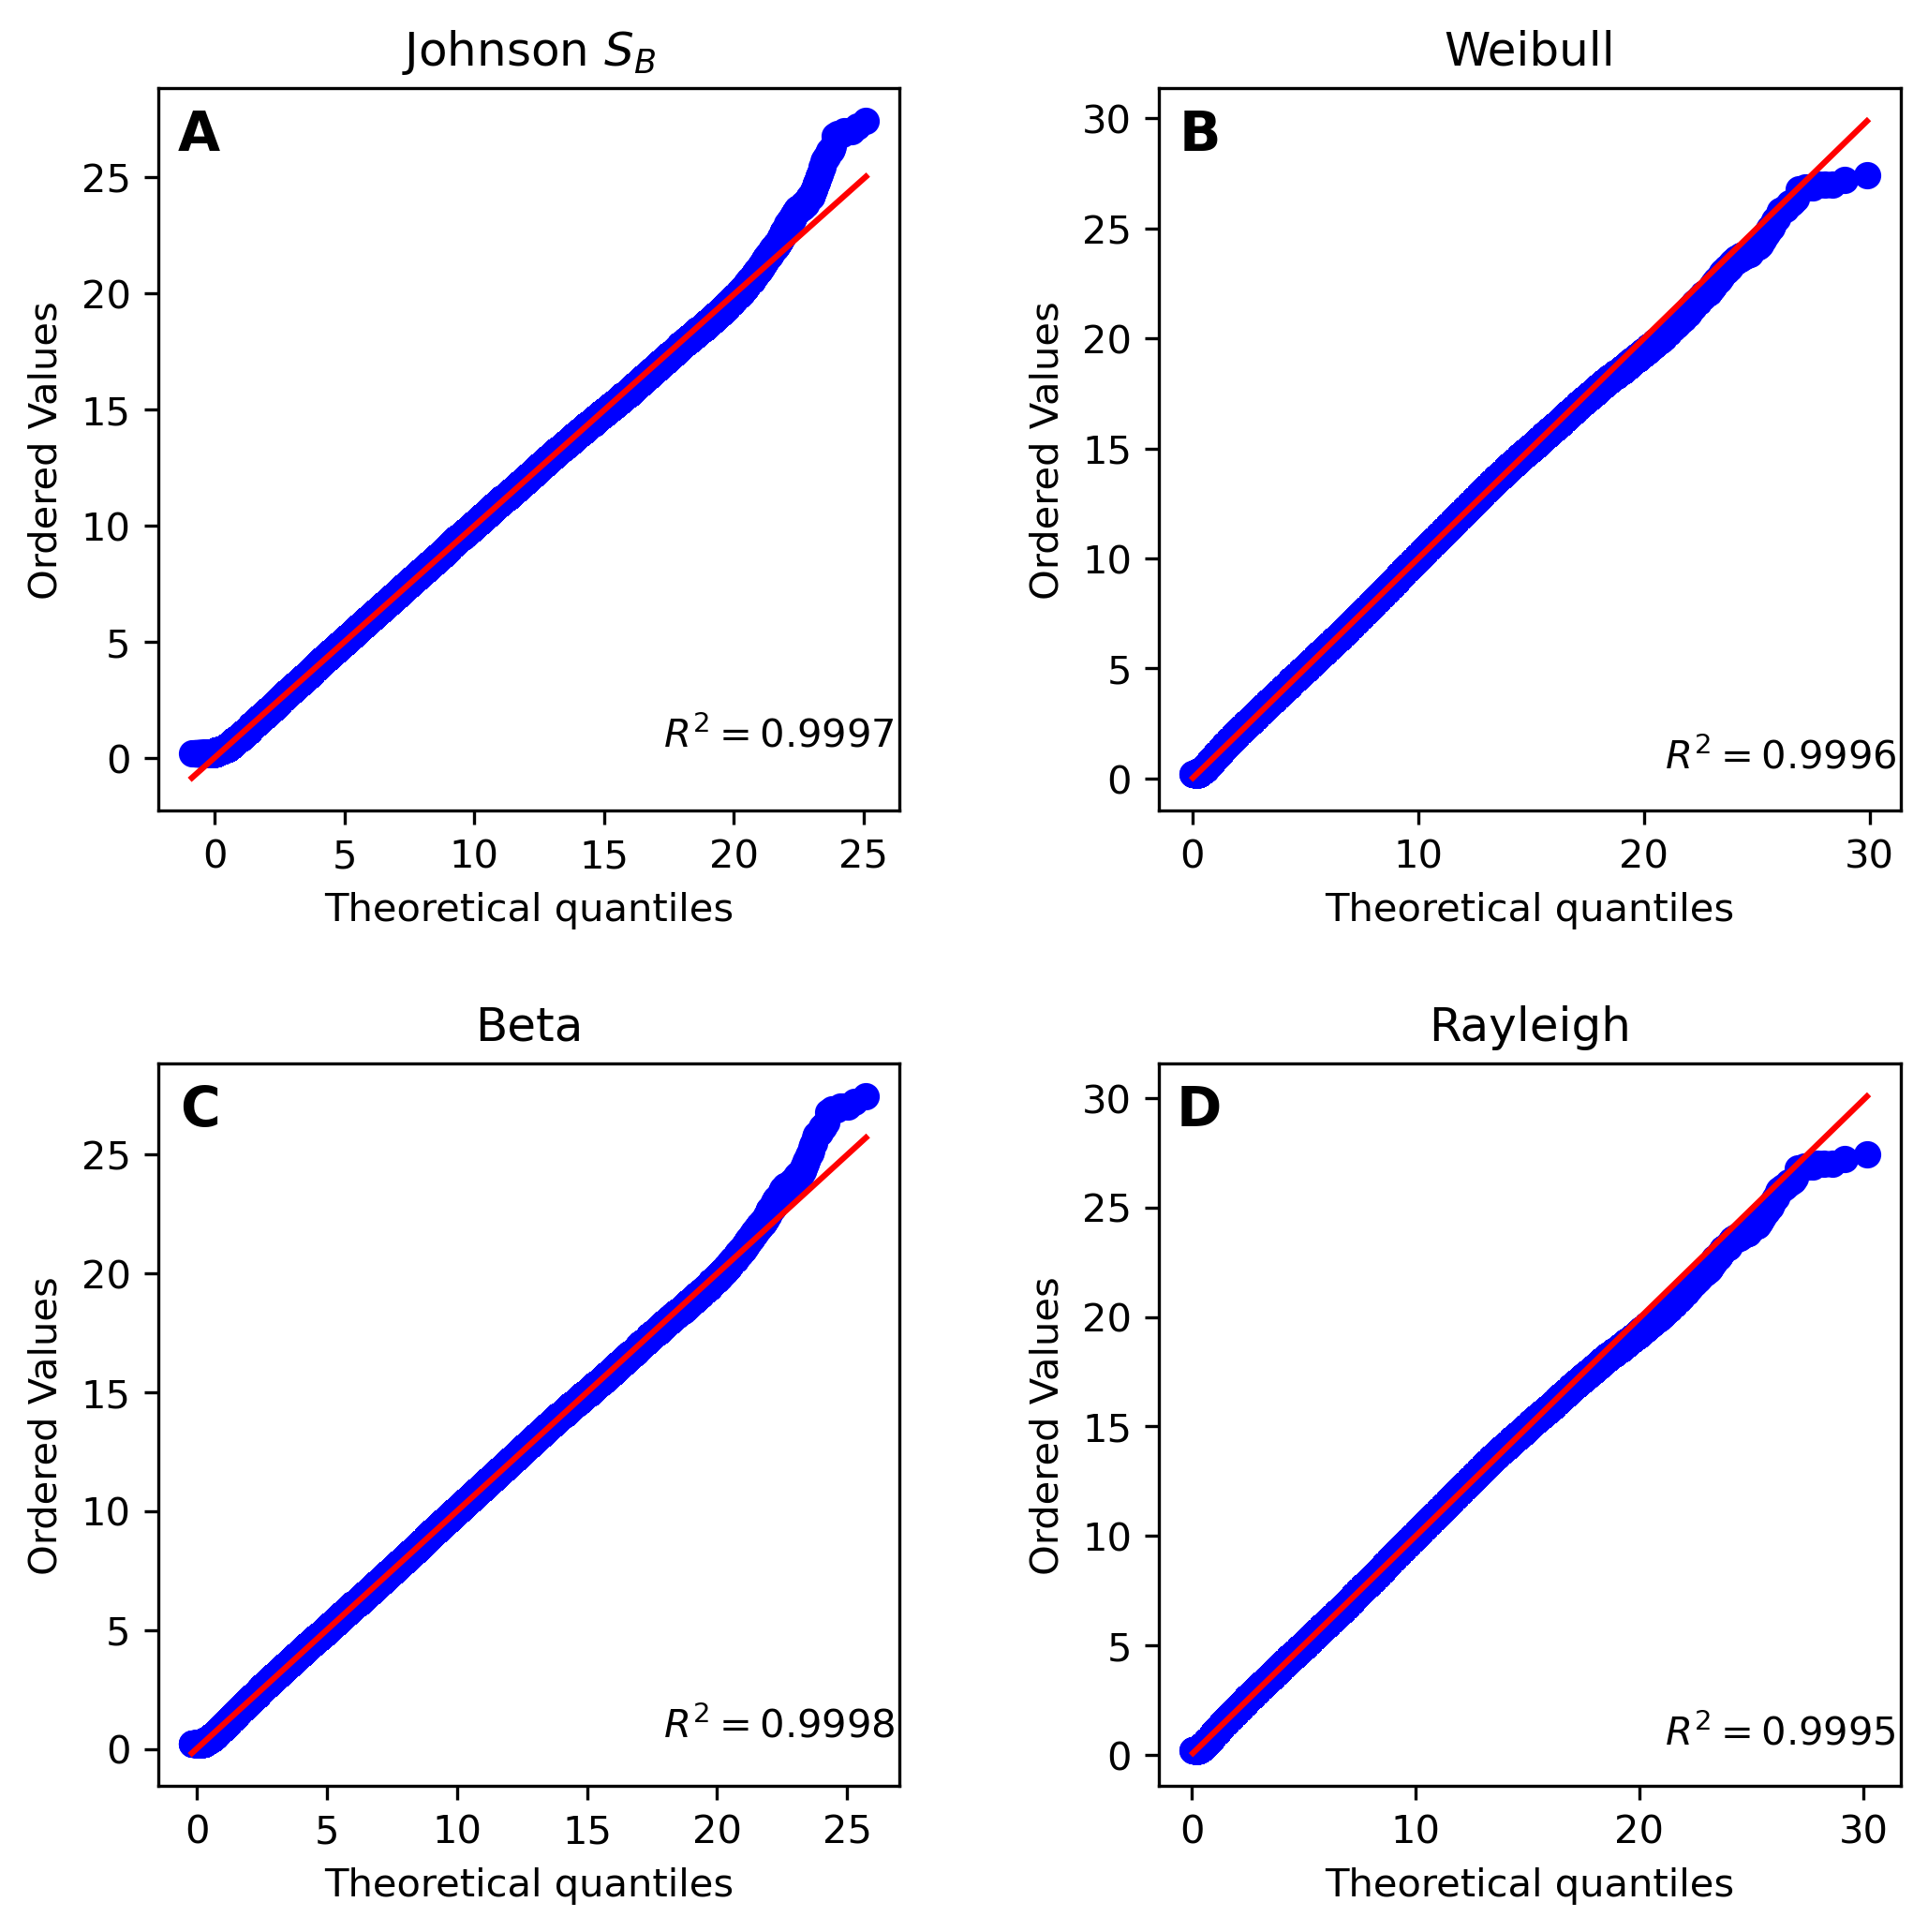
\includegraphics[width=0.68\linewidth]{Figures/Chapter5/b44025_wind_probplot.png}
%\decoRule
\caption{Buoy 44025 $u_{10}$ probability plots and the corresponding coefficient of determination for each PDF.}
\label{fig:b44025_probplot}
\end{figure}


\begin{figure}[H]
\centering
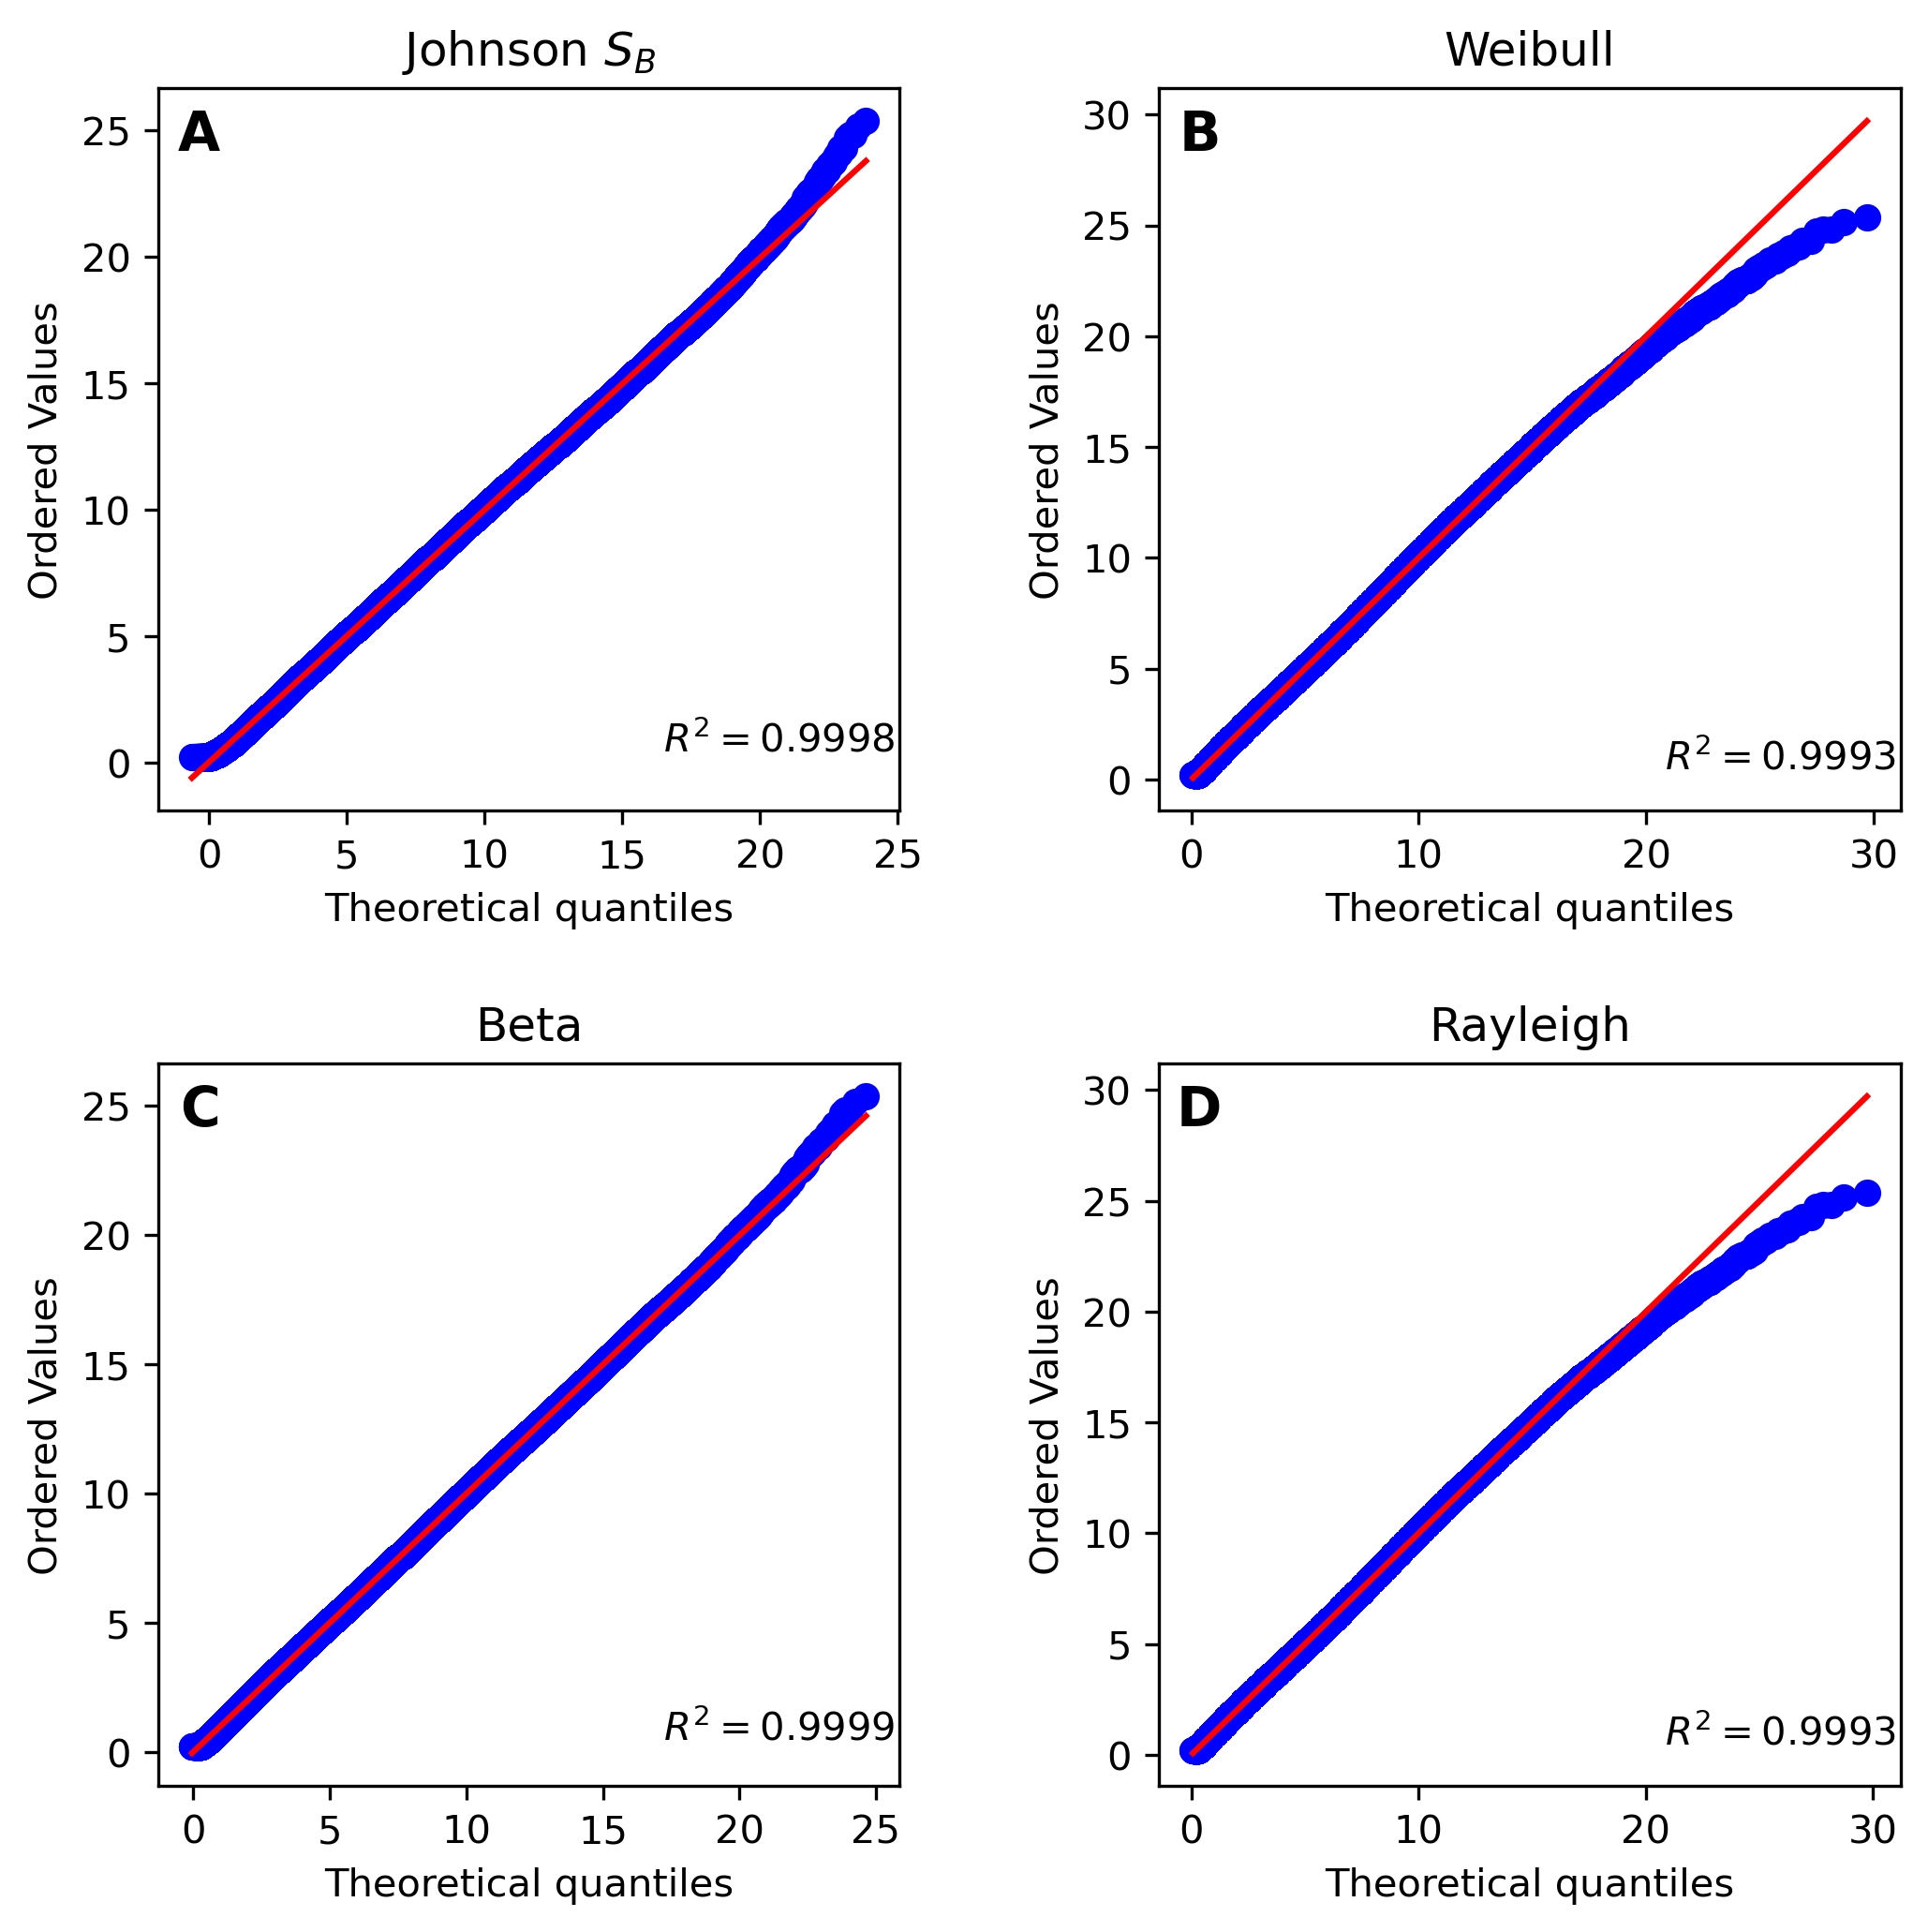
\includegraphics[width=0.68\linewidth]{Figures/Chapter5/b44017_wind_probplot.png}
%\decoRule
\caption{Buoy 44017 $u_{10}$ probability plots and the corresponding coefficient of determination for each PDF.}
\label{fig:b44017_probplot}
\end{figure}


\begin{figure}[H]
\centering
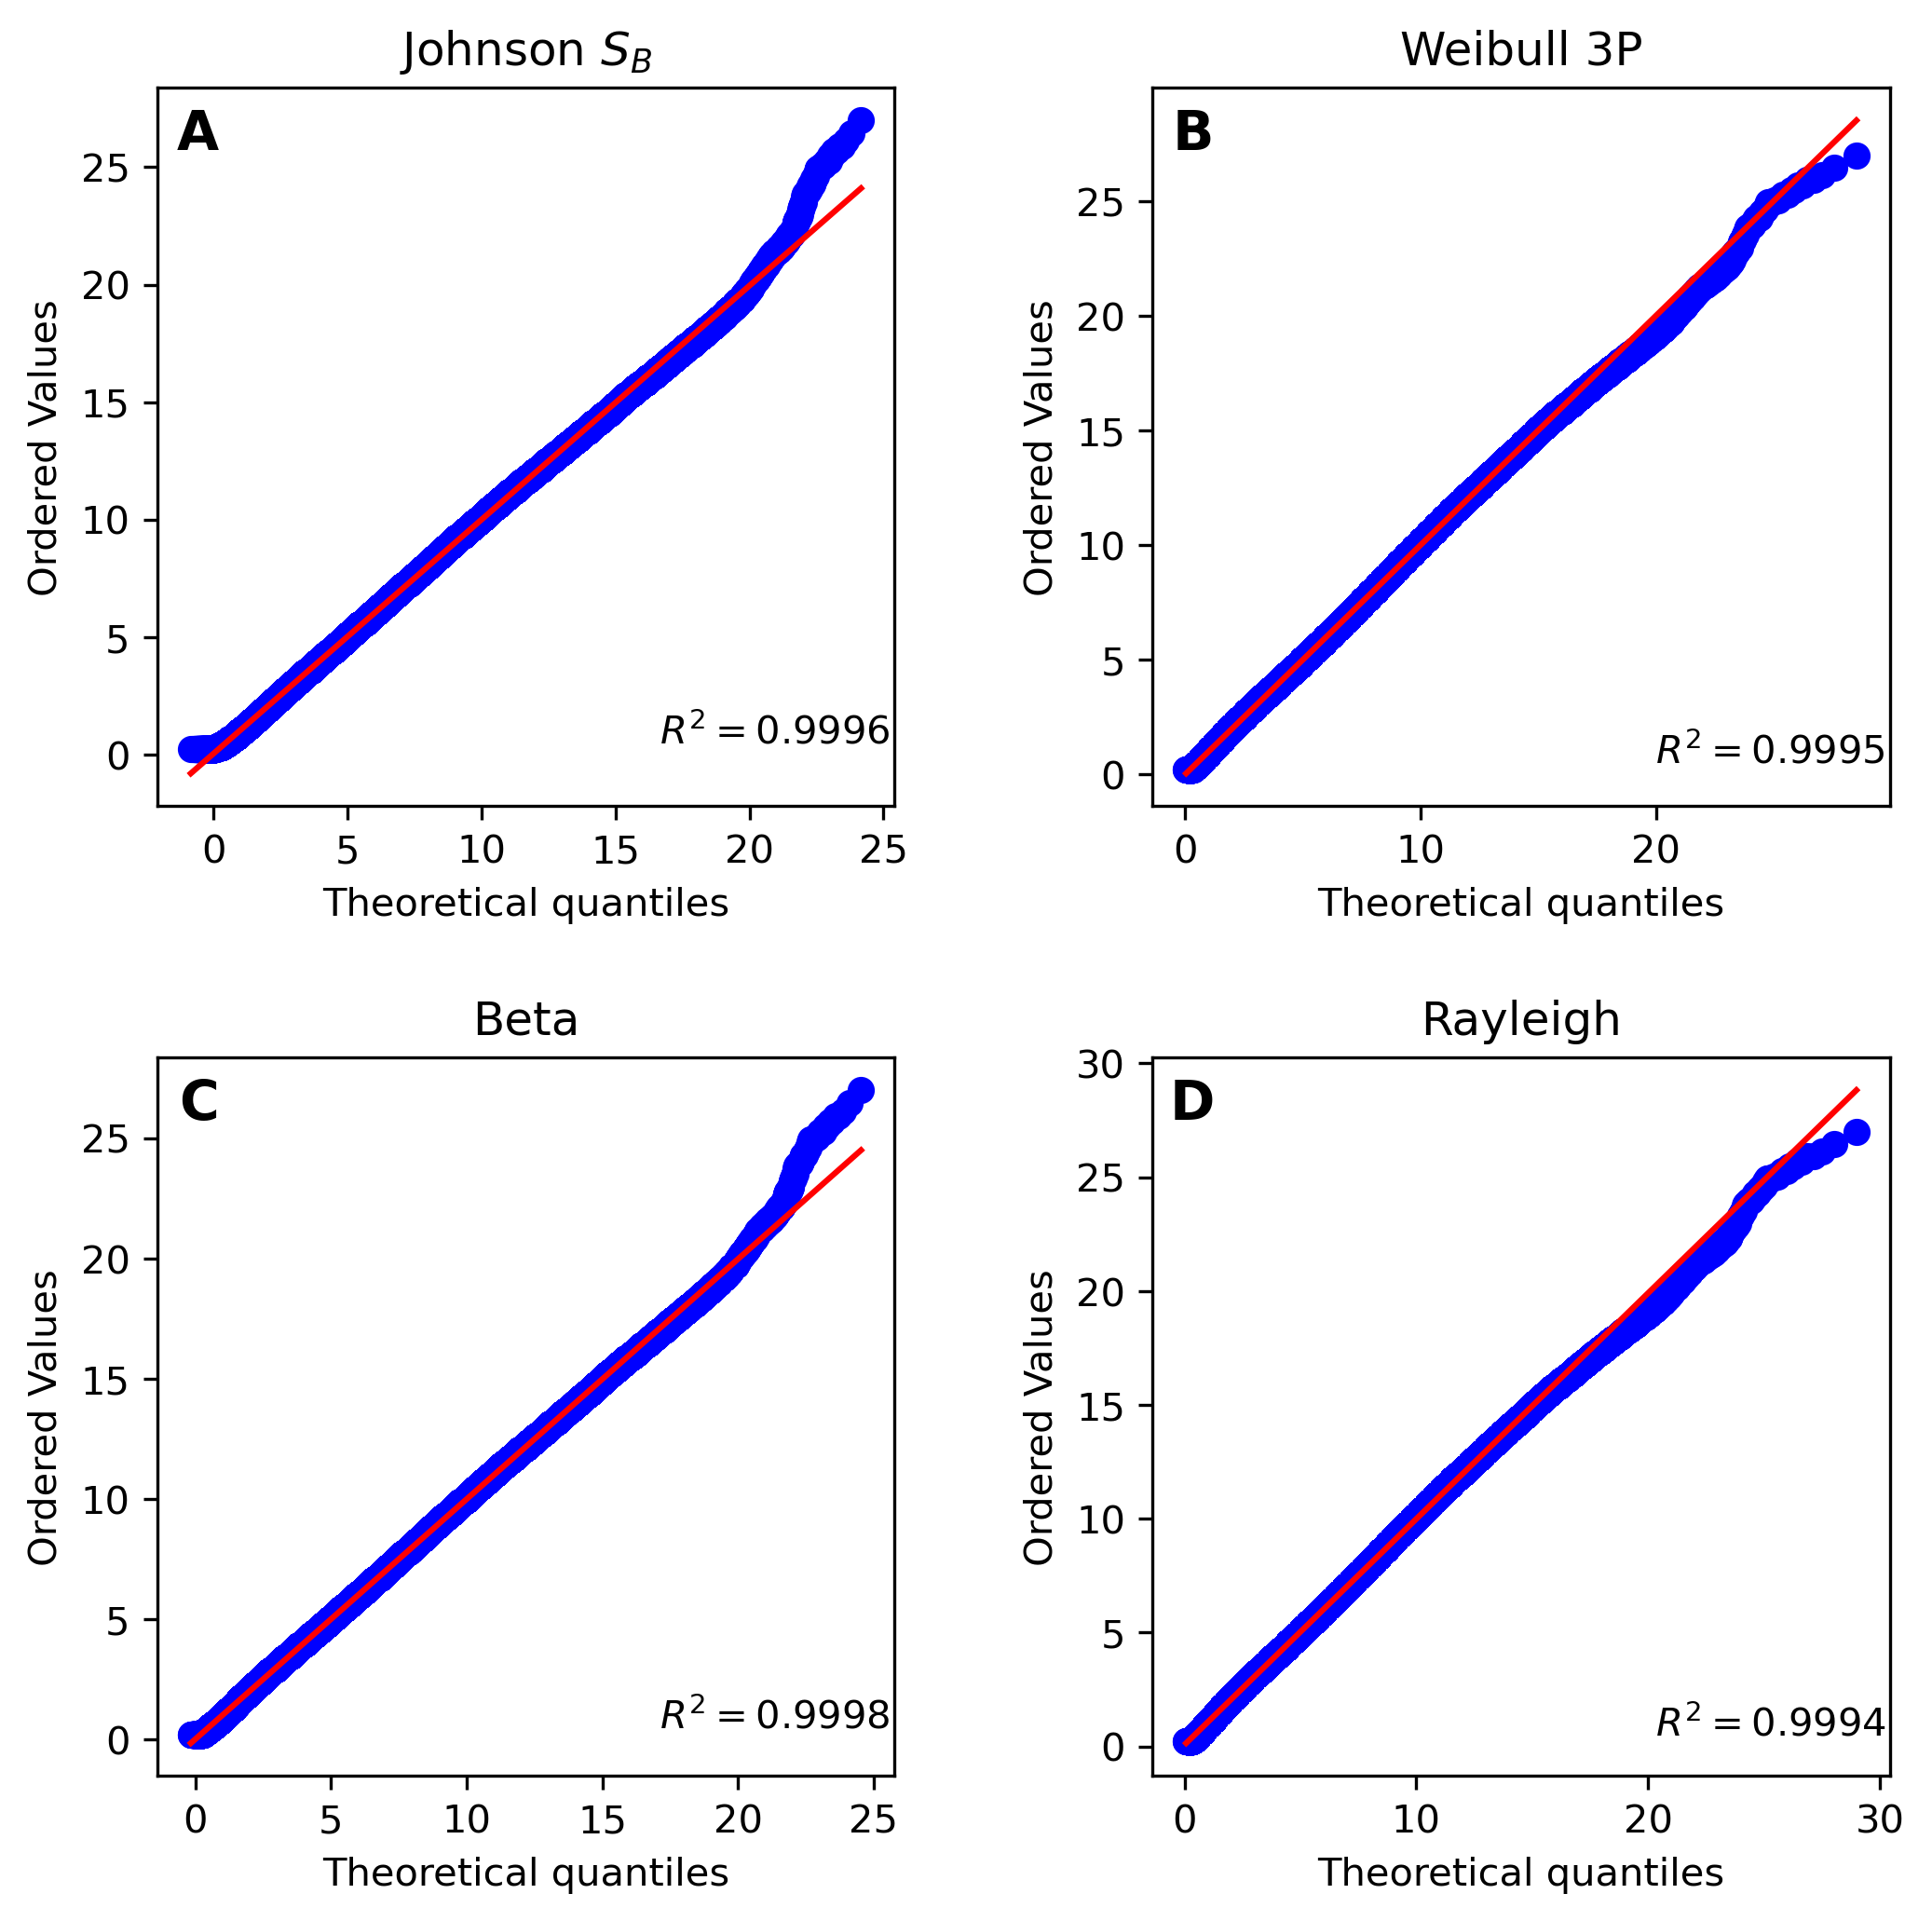
\includegraphics[width=0.68\linewidth]{Figures/Chapter5/b44065_wind_probplot.png}
%\decoRule
\caption{Buoy 44065 $u_{10}$ probability plots and the corresponding coefficient of determination for each PDF.}
\label{fig:b44065_probplot}
\end{figure}



\begin{figure}[H]
\centering
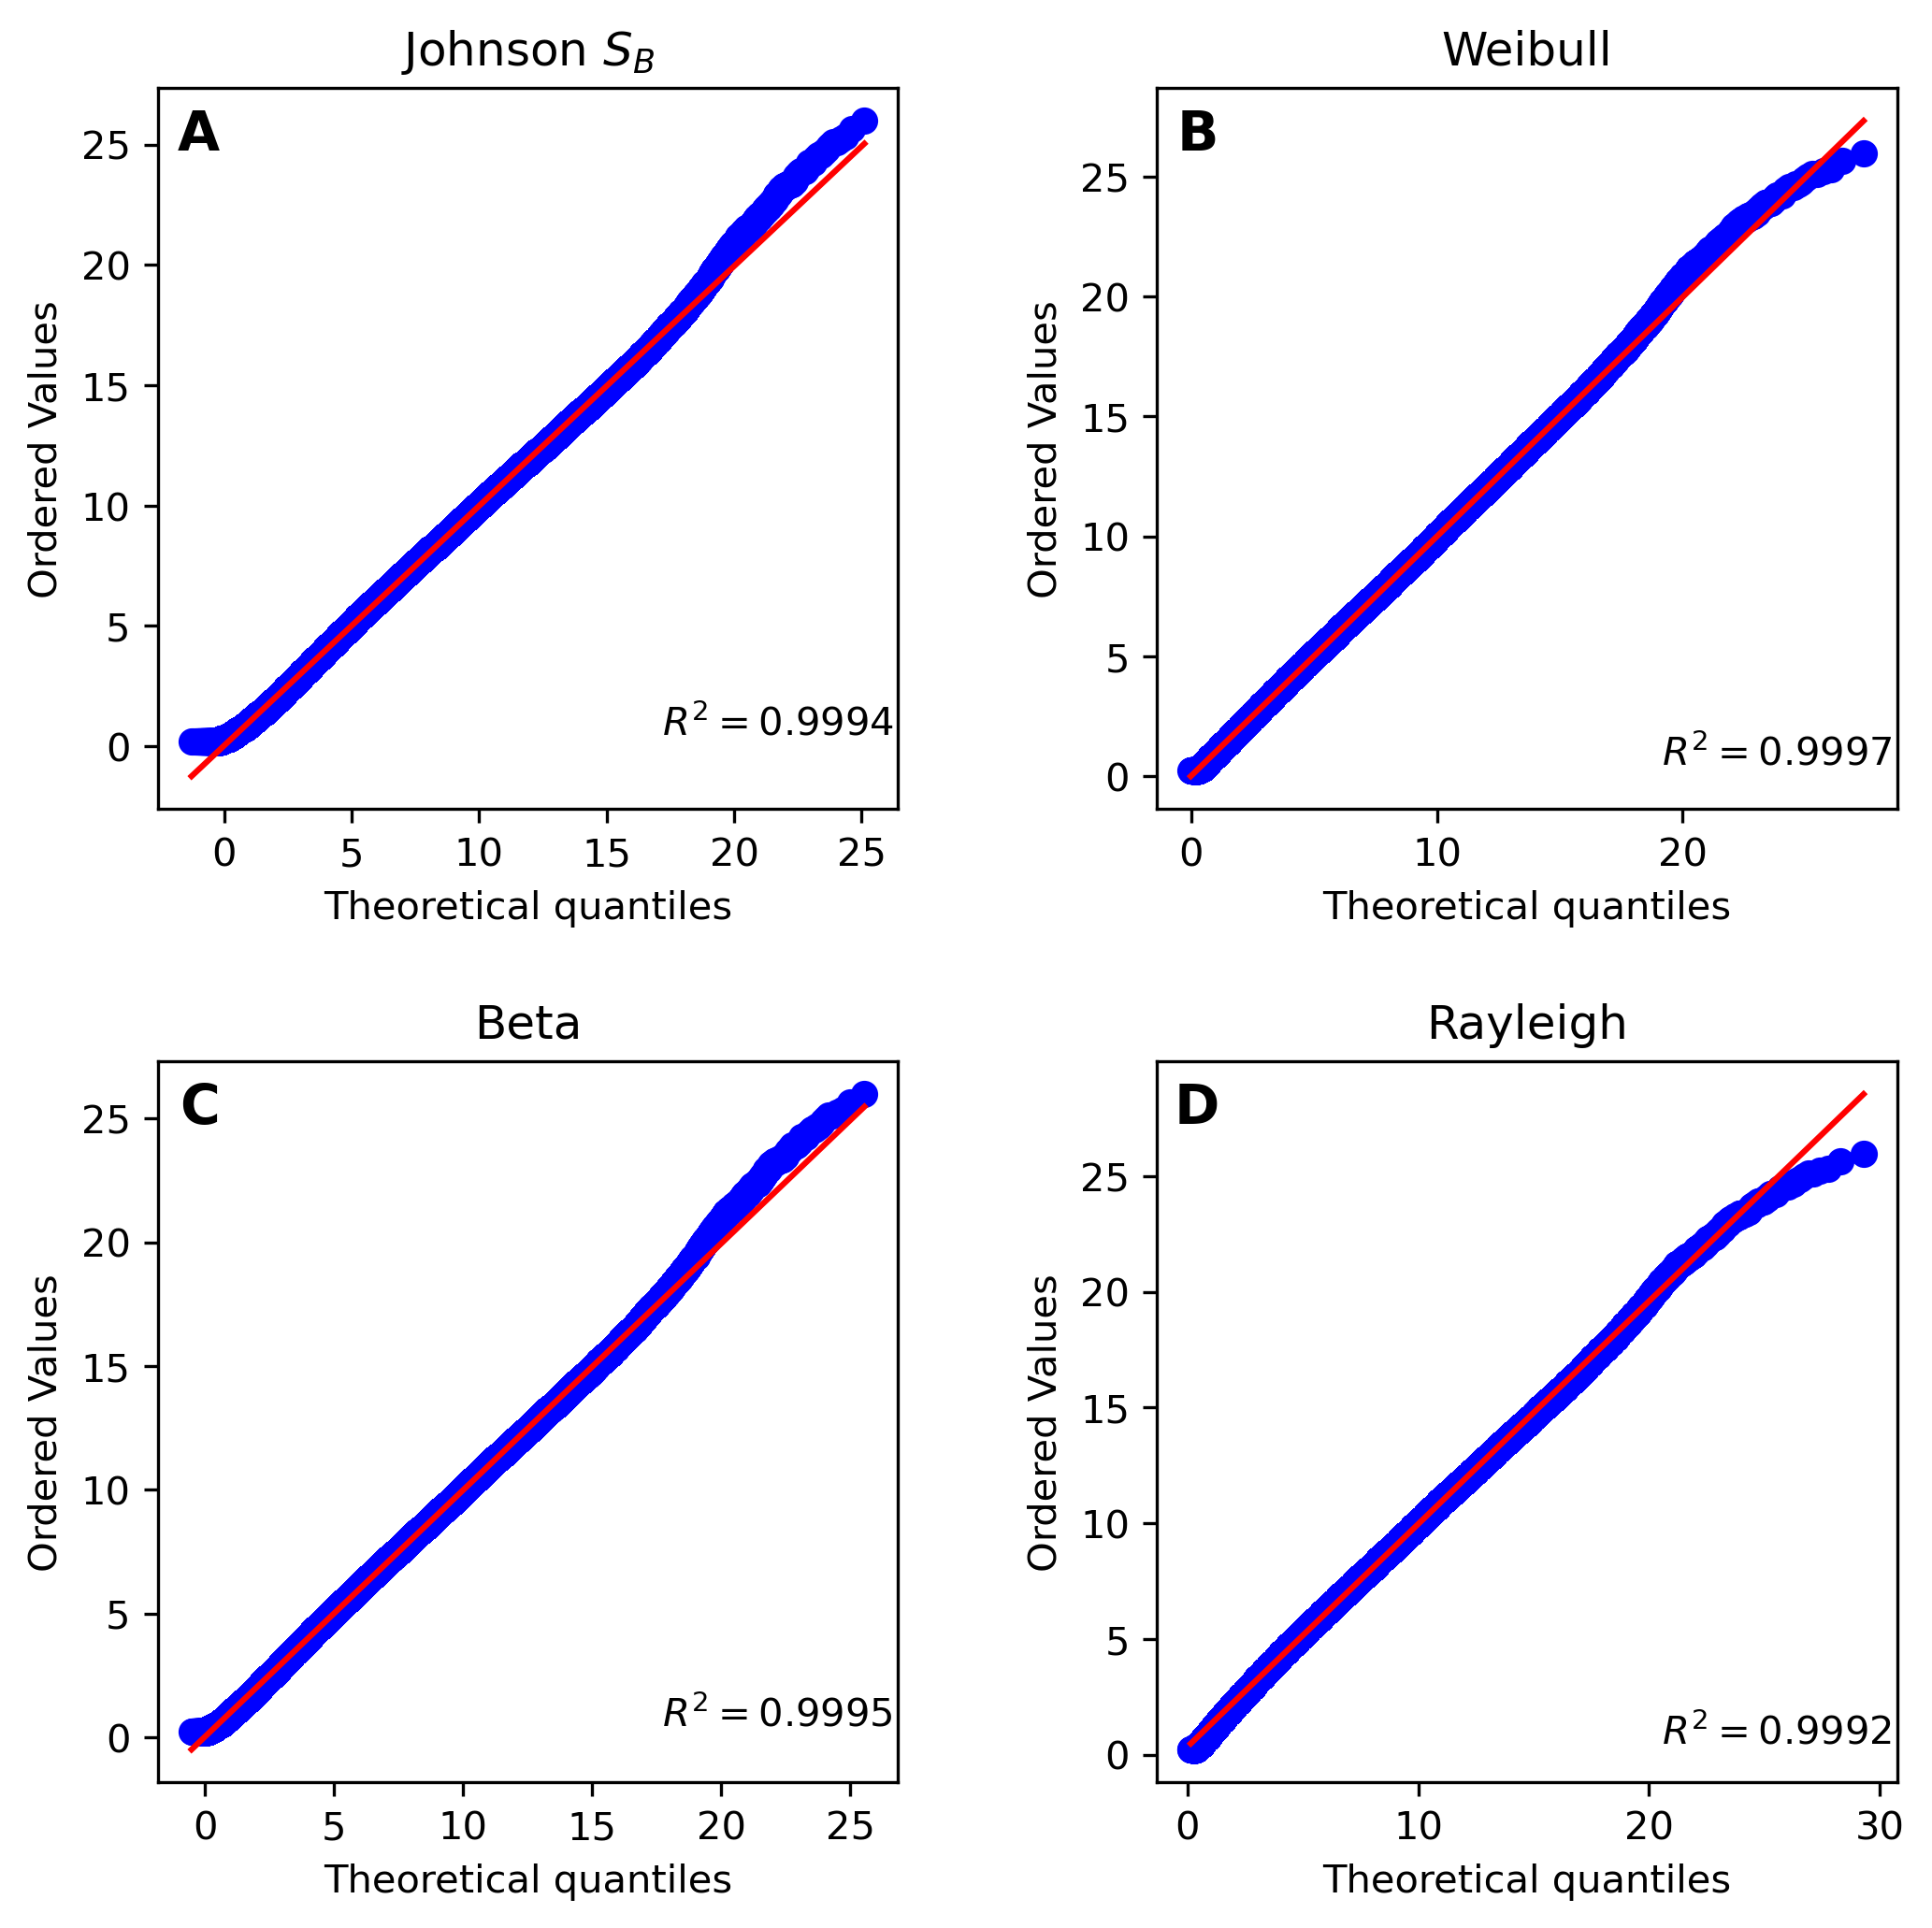
\includegraphics[width=0.68\linewidth]{Figures/Chapter5/b44020_wind_probplot.png}
%\decoRule
\caption{Buoy 44020 $u_{10}$ probability plots and the corresponding coefficient of determination for each PDF.}
\label{fig:b44020_probplot}
\end{figure}





\begin{figure}[H]
\centering
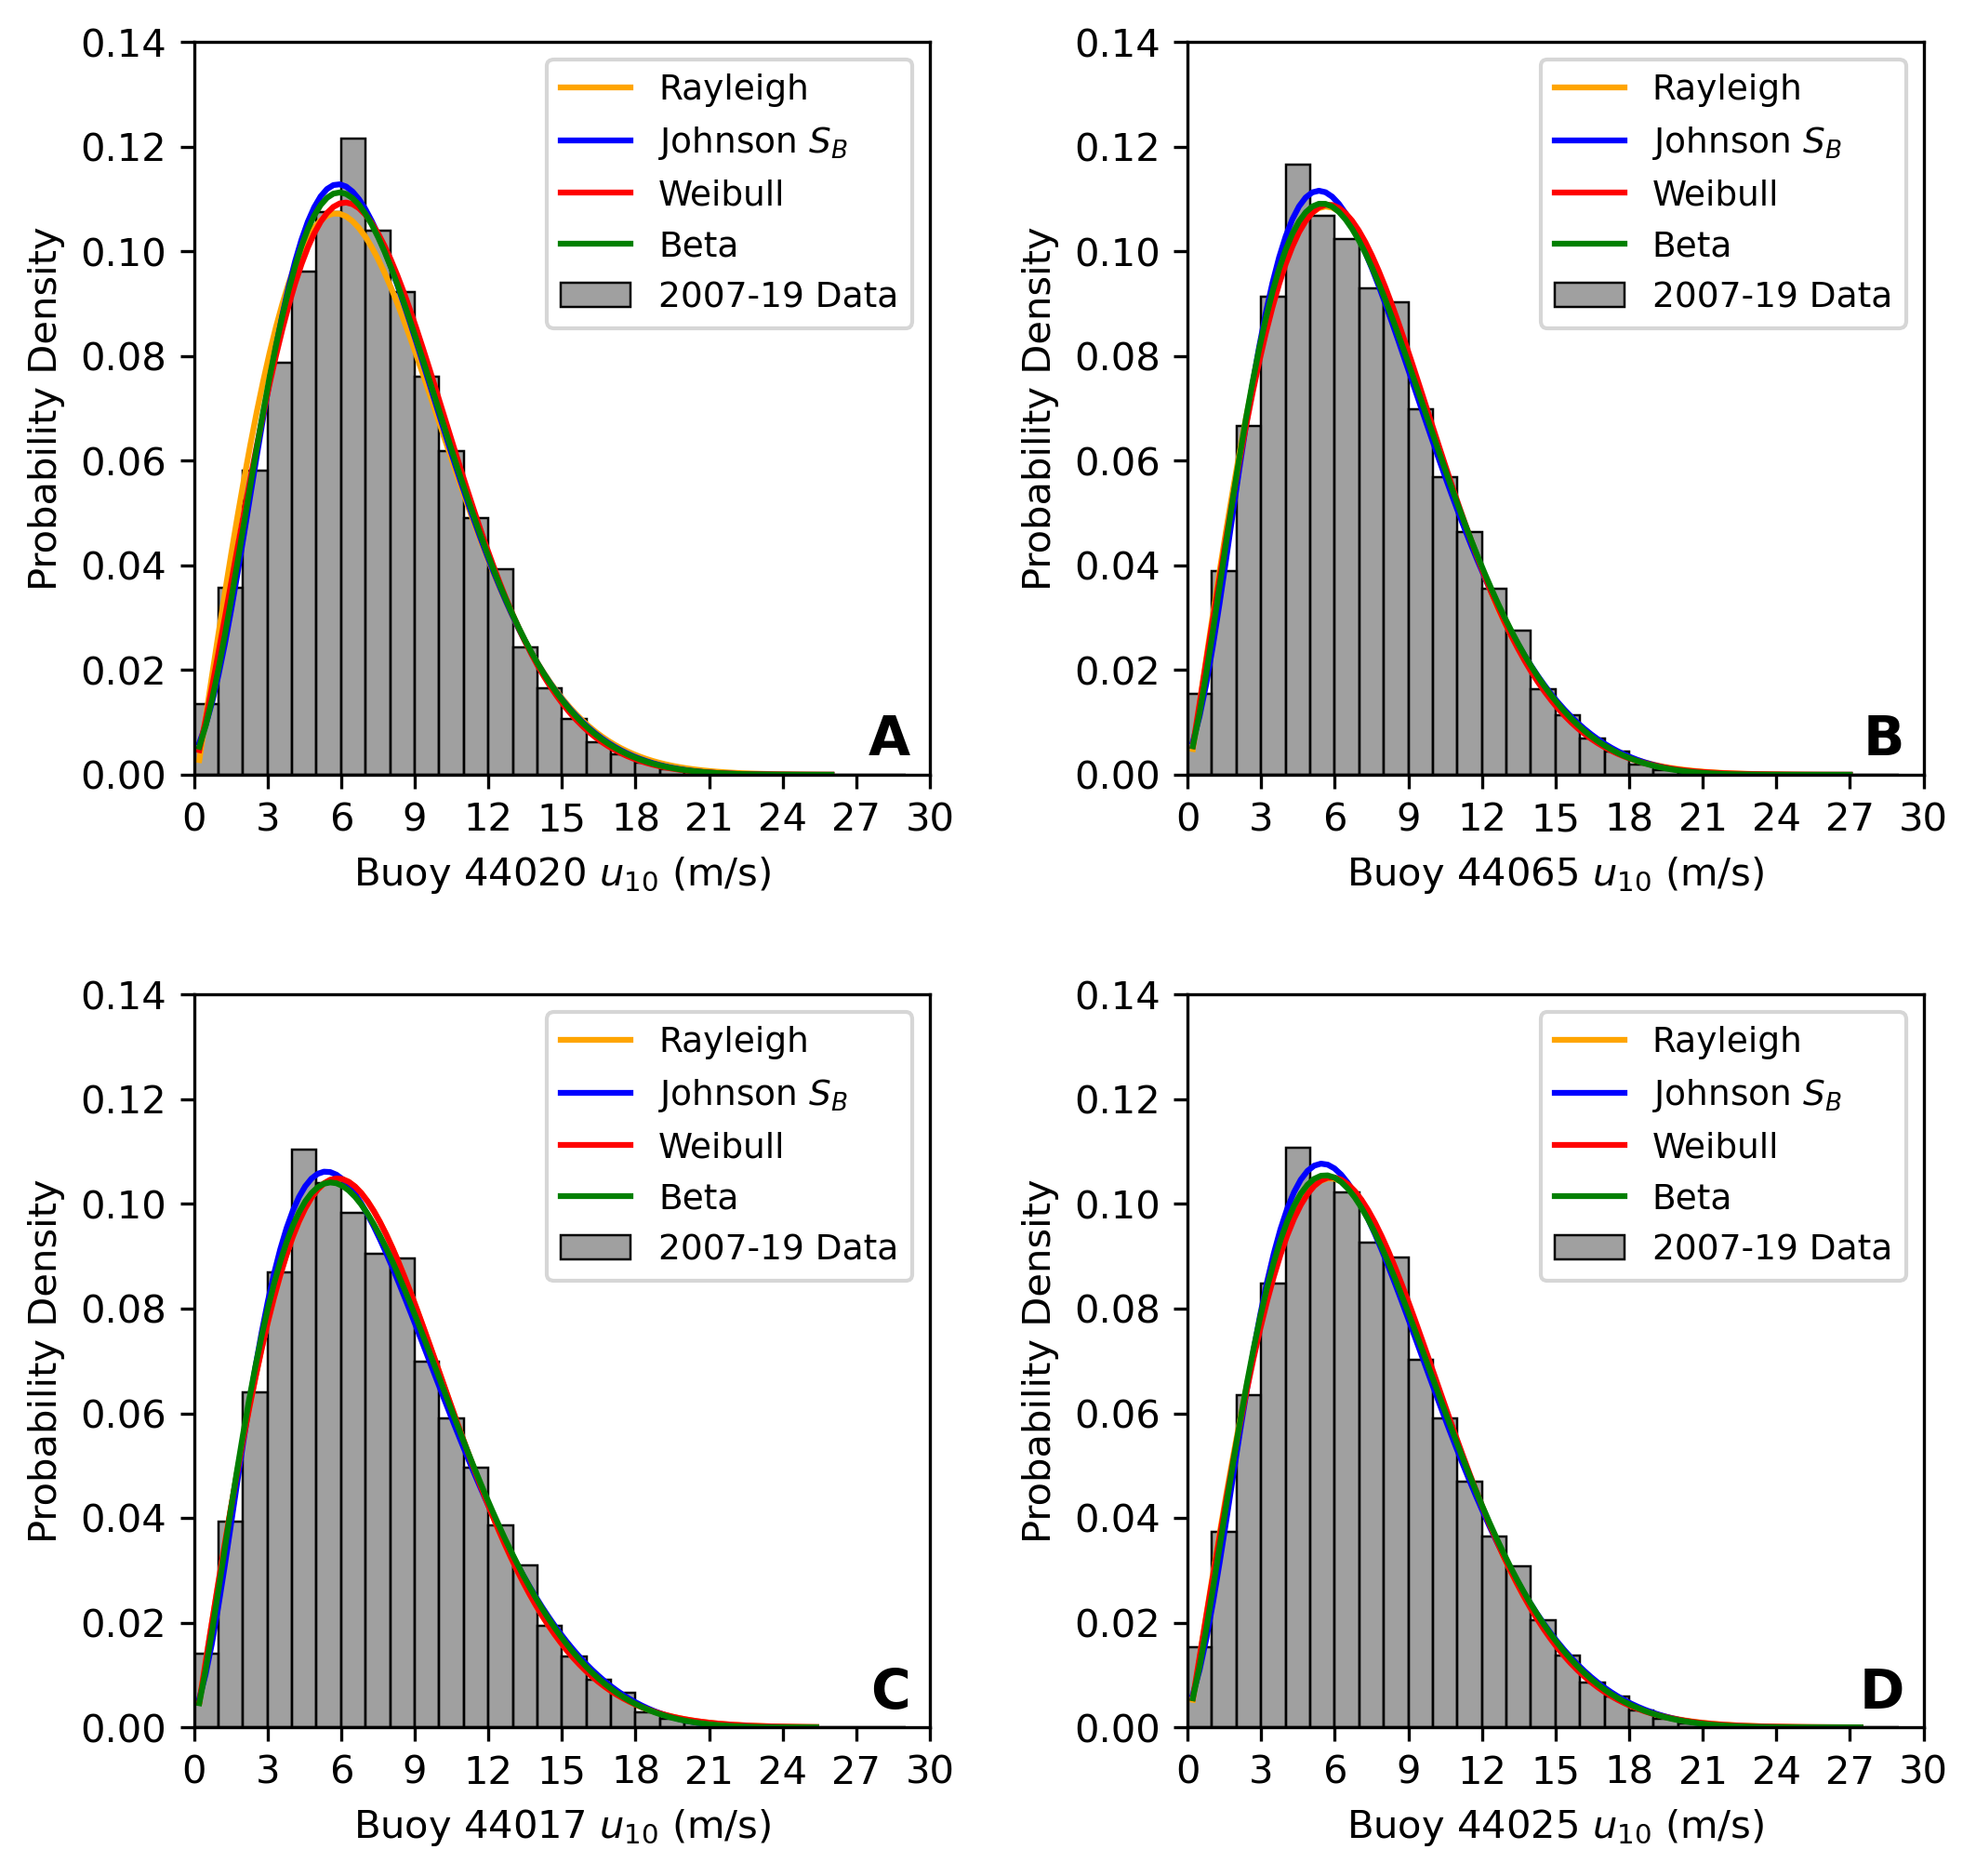
\includegraphics[width=0.95\linewidth]{Figures/Chapter5/wind_pdfs_loc1.png}
%\decoRule
\caption{$u_{10}$ histograms and the four PDFs that provide the best fit to the buoy data.}
\label{fig:pdfs_wind}
\end{figure}





\pagebreak

\section{Wind Speed and Wave Height Relationships}

The theoretical formulas which connect $u_{10}$ with $H_{s}$ are available in \ref{wind_wave_relationships}. In this study, the wind-wave relationships are estimated using a second-degree polynomial regression fitting of the SWH to the $u_{10}$ adjusted values. Previous studies, dedicated to the East Coast of the United States, use more sophisticated methods \cite{Andreas2007}. This study attempts to integrate and interpret the difference between the wind-wave relationships depending on the wind direction for every location. Specifically, the eight major directions, each with an angular window of 45 degrees, are used. All figures include the sample size and the estimated coefficients of the fitted line. 



\begin{figure}[H]
\centering
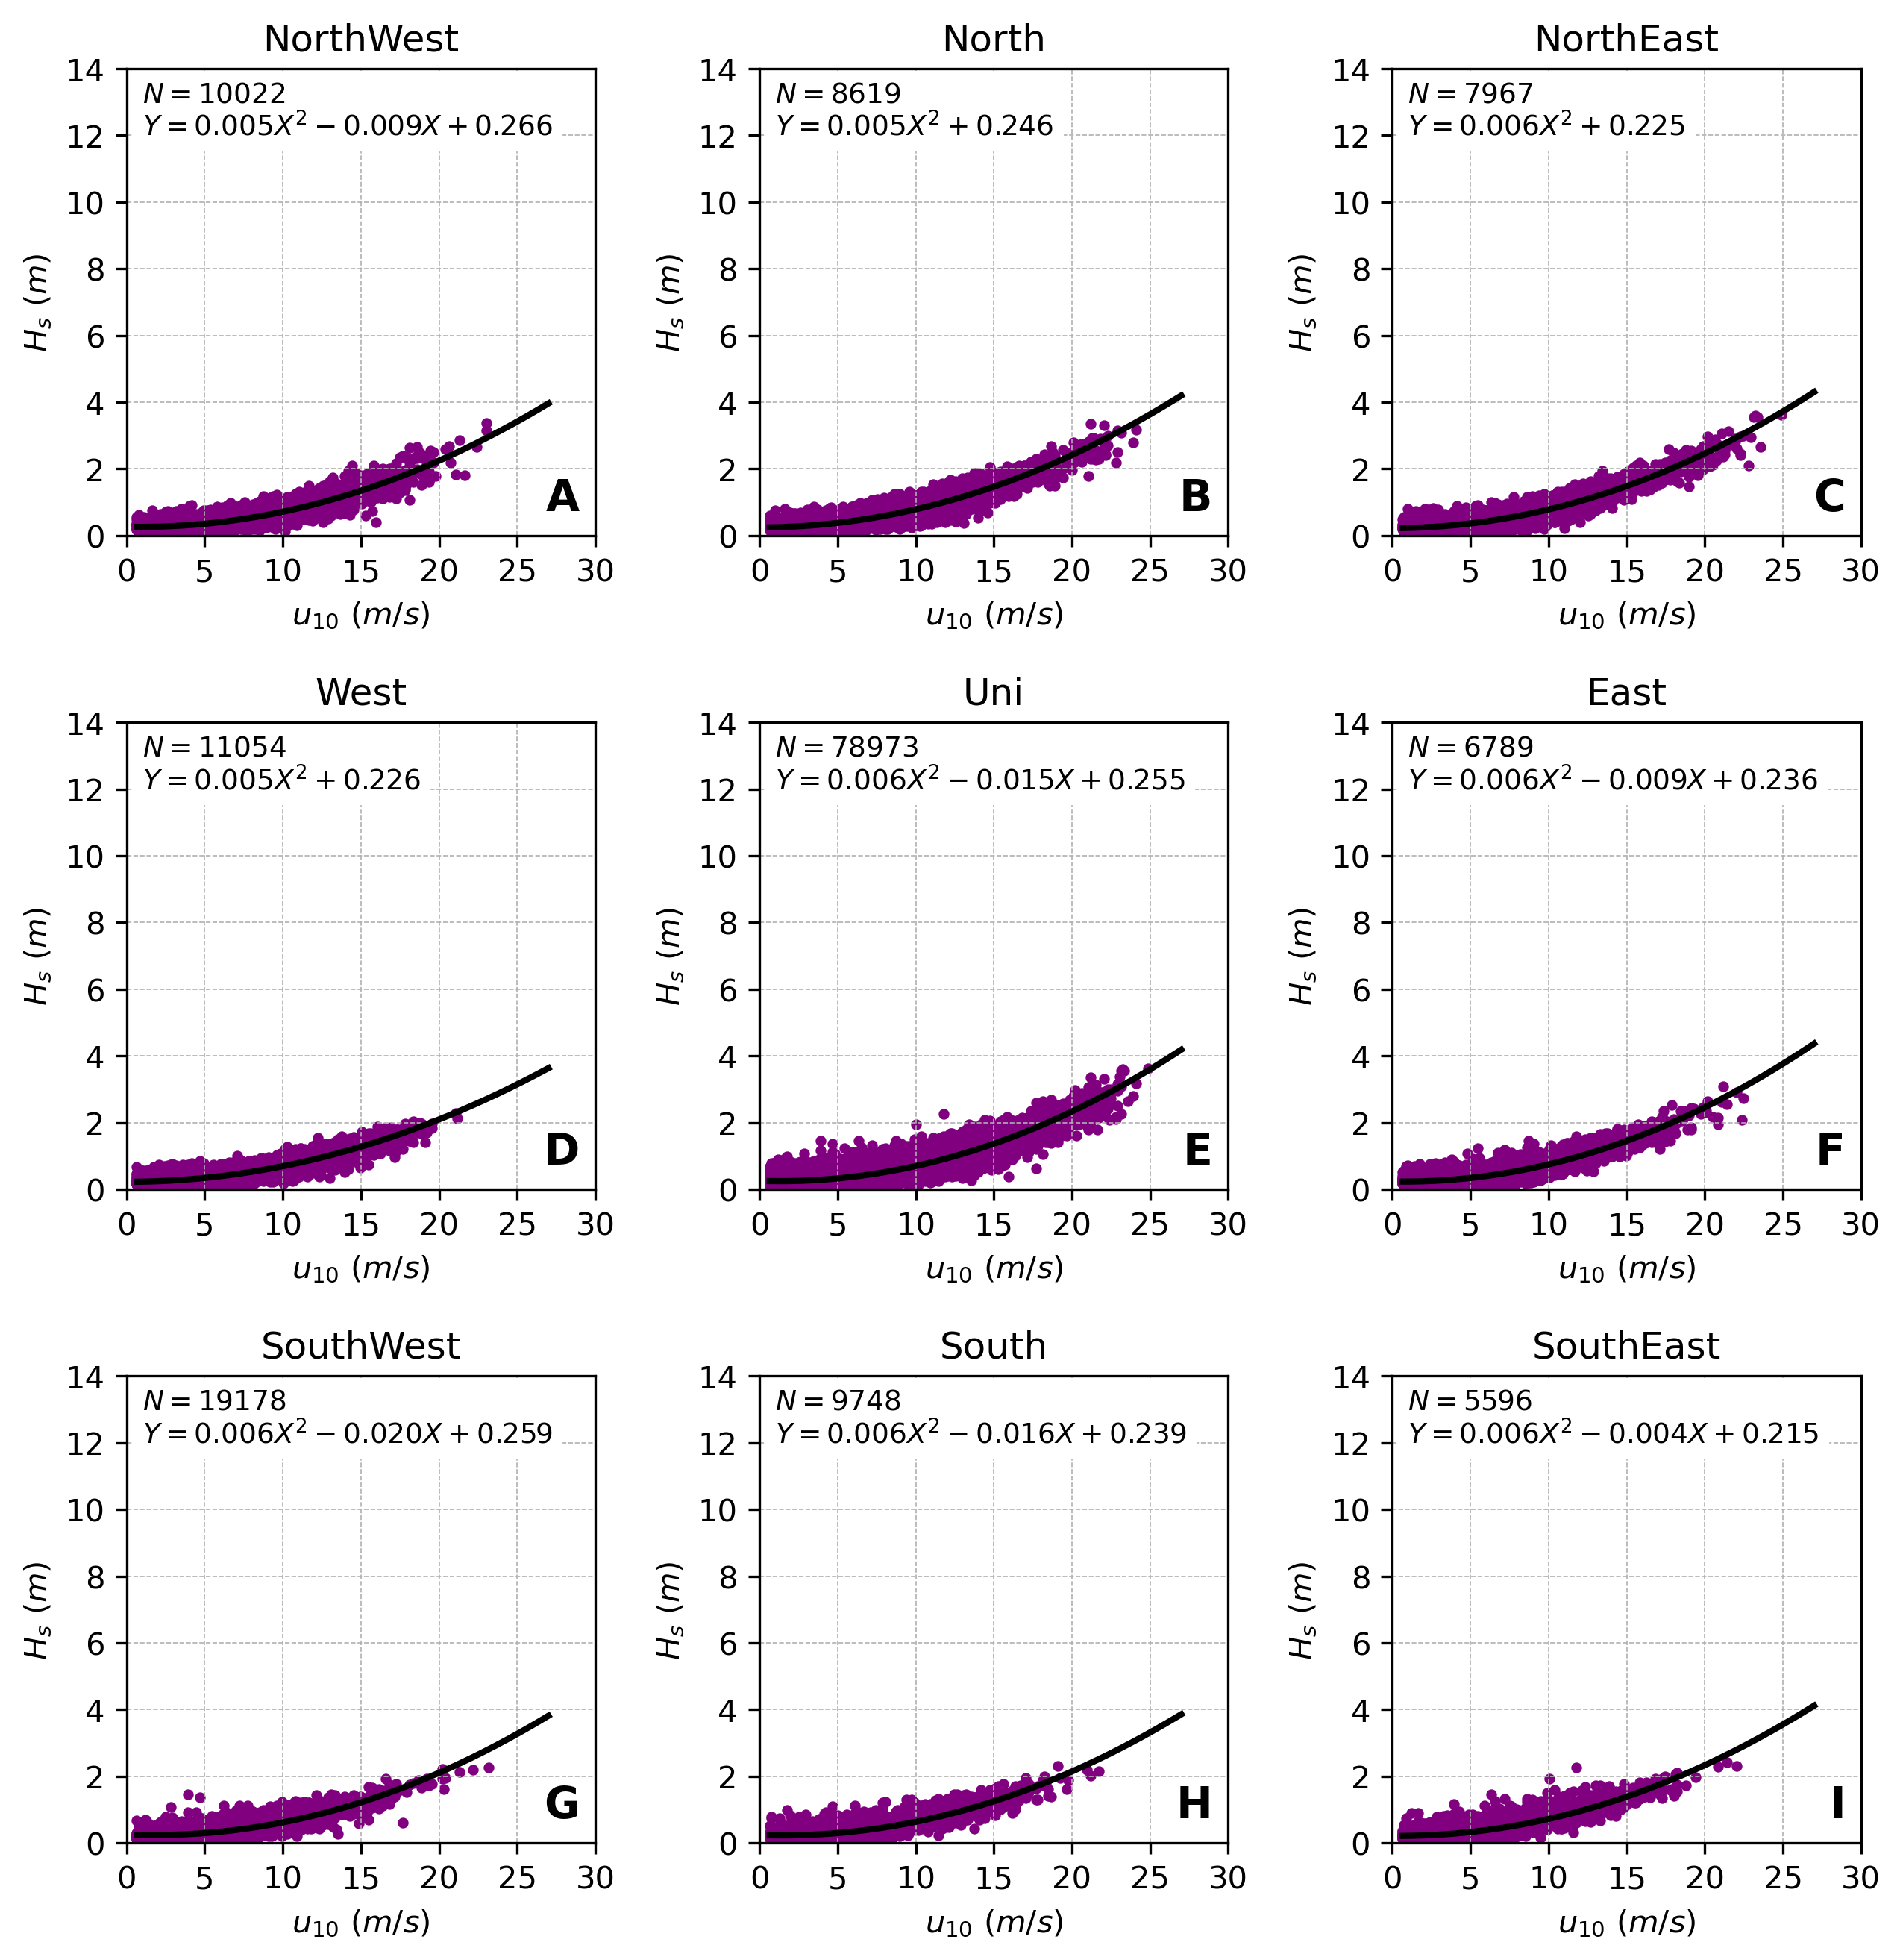
\includegraphics[width=0.95\linewidth]{Figures/Chapter5/b44020_wind_wave.png}
%\decoRule
\caption{Buoy 44020 wind wave relationships for each of the main wind directions and for all directions combined (E).}
\label{fig:wind_wave_44020}
\end{figure}


Figure~\ref{fig:wind_wave_44020} indicates the strength of the relationship. The sheltered buoy 44020 is surrounded by the southeastern Massachusetts and the Martha’s Vineyard, Nantucket islands. The only opening for the entrance of swell waves in the region is from the east. Hence, wind waves dominate the region throughout the year. The relationships fit exceptionally the data with a minimal number of outliers. Even the highest waves that are coming from the northeast and north directions are well-captured by such relationships. Generally, the coefficients are consistent for every wind direction, except for the west, north, and northeast directions, where the second coefficient is zero. The small intercept is an indication of the minimal influence of swells in the region.


\begin{figure}[H]
\centering
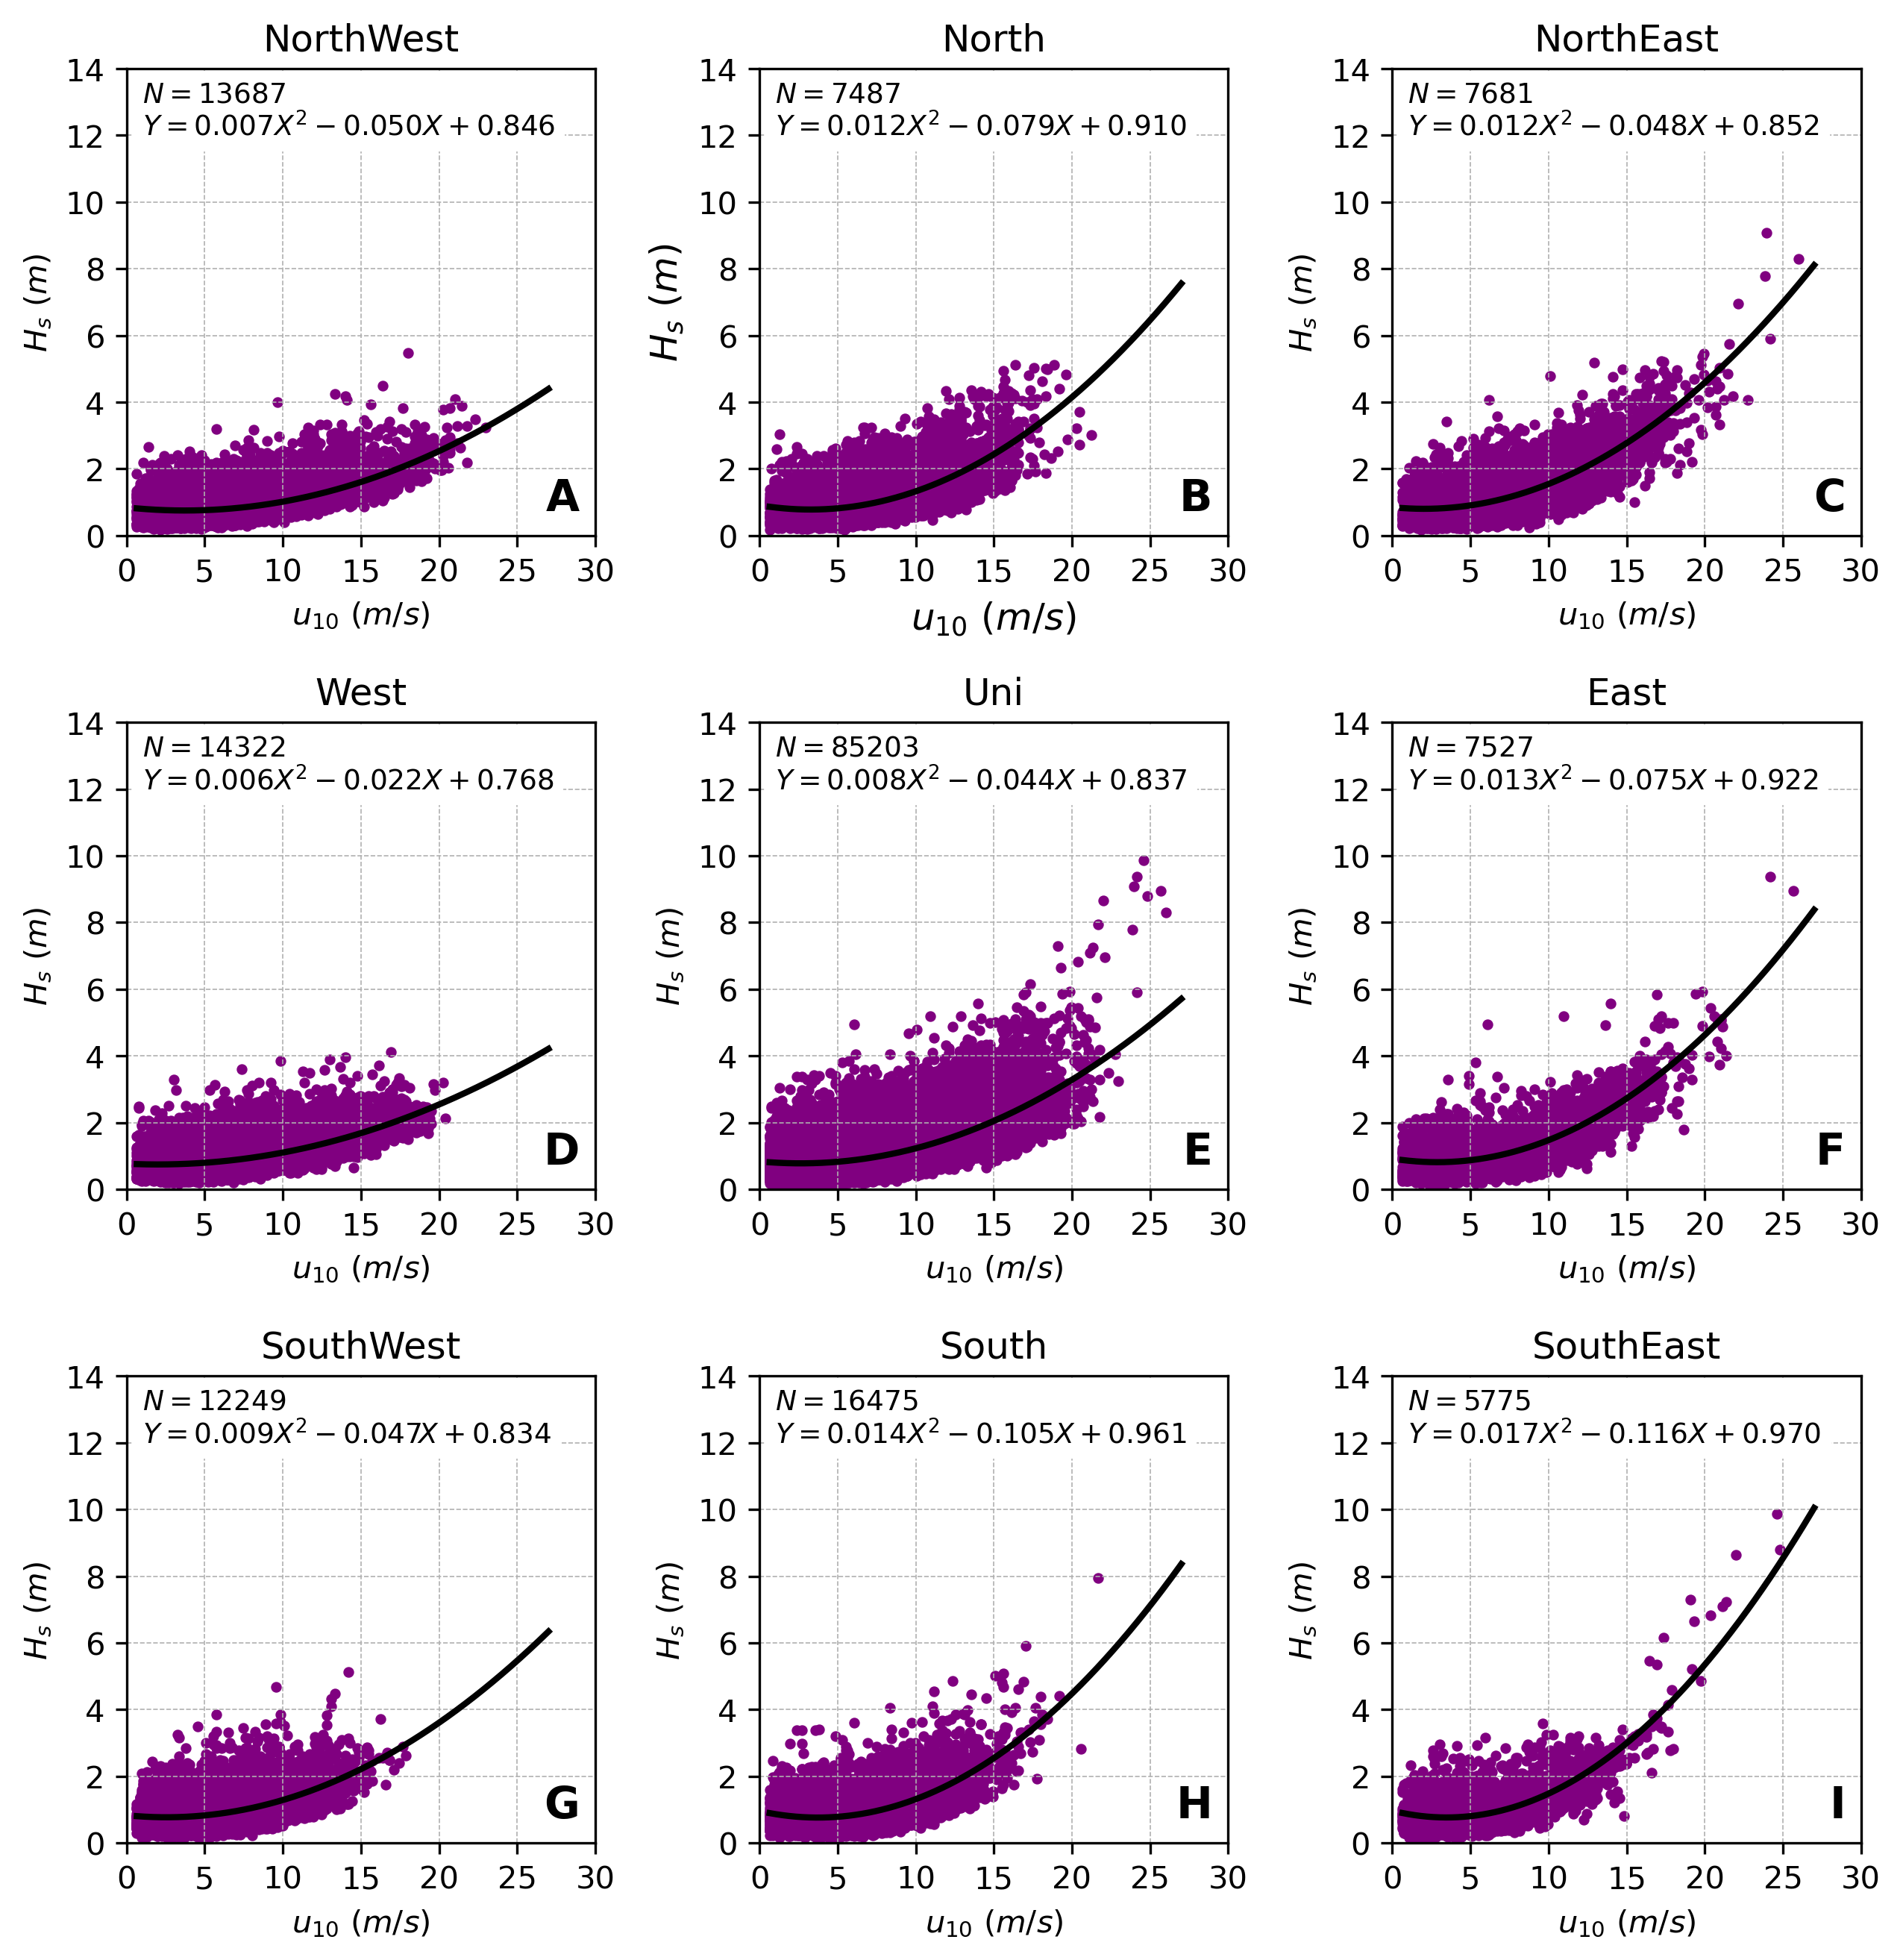
\includegraphics[width=0.95\linewidth]{Figures/Chapter5/b44065_wind_wave.png}
%\decoRule
\caption{Buoy 44065 wind wave relationships for each of the main wind directions and for all directions combined (E).}
\label{fig:wind_wave_44065}
\end{figure}


On the contrary, this is not the case for the open-ocean buoy 44008, as it is located in a swell-dominated region, although its distance from the sheltered buoy is just 50 kilometers approximately. The range of the $H_{s}$ values is substantial, even for low wind speeds, increasing the uncertainty of its estimation when only the $u_{10}$ is given. The coefficients also vary depending on the wind direction. In directions with higher wind speeds and potential for producing higher sea states, the coefficients tend to be larger, as the northeast and east directions.
Besides, an interesting feature of the coastal buoy relationships is that when the wind is aligned with the swell direction (from the east to the south), the second coefficient is significantly larger, almost ten times the same coefficients of the relationships for the western wind direction, which is the most common for every location in SNE throughout the year. The above means that on conditions of very light winds speeds (0-5 m/s), the $H_{s}$ becomes smaller with increasing wind speed. This feature is not present in the sheltered buoy relationship. We may connect this behavior with the upward momentum transfer described in \cite{Grachev2001}, but it requires further investigation.


\begin{figure}[H]
\centering
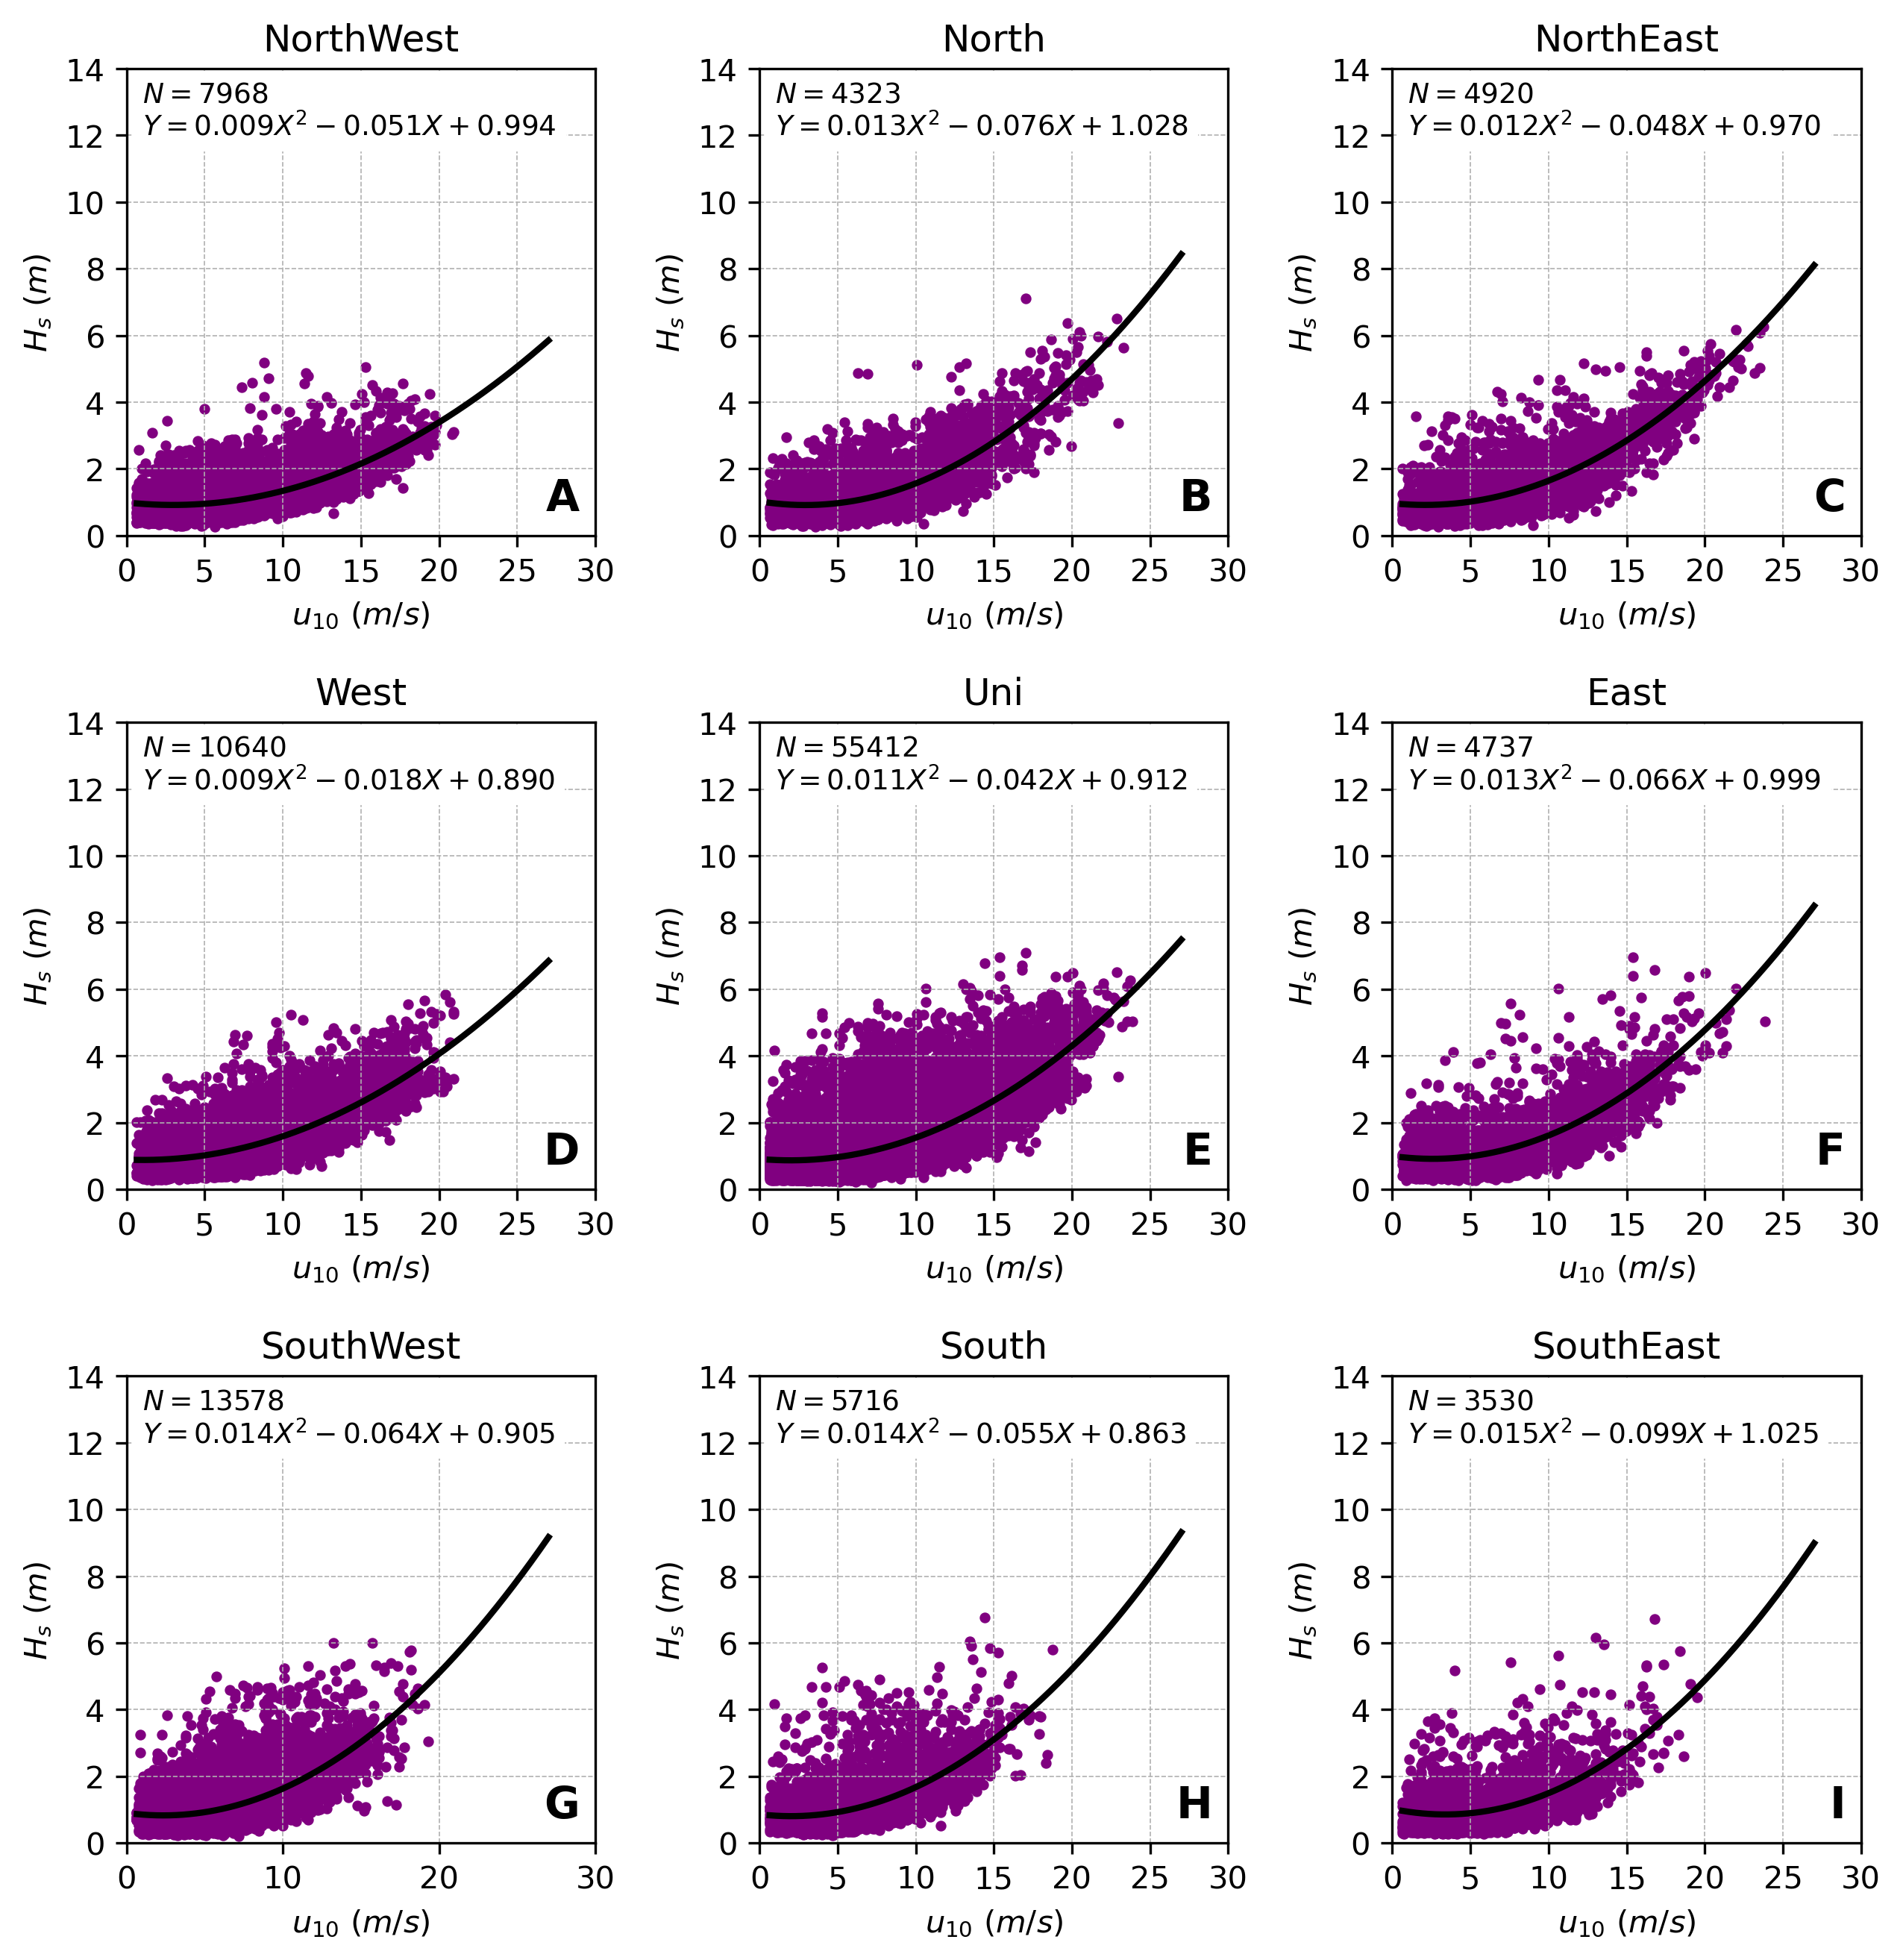
\includegraphics[width=0.95\linewidth]{Figures/Chapter5/b44017_wind_wave.png}
%\decoRule
\caption{Buoy 44017 wind wave relationships for each of the main wind directions and for all directions combined (E).}
\label{fig:wind_wave_44017}
\end{figure}


Finally, Figure~\ref{fig:wind_wave_buoys} shows a comparison of the estimated relationships for the whole time series record of each buoy. The increasing curvature of the lines of best fit with increasing distance from the coast is expected. It is also worth mentioning that the adjacent coastal buoys 44025 and 44017 located south of the Long Island Sound show almost identical relationships. Again, it is necessary to highlight the increased uncertainty of the relationships and their reduced capability to describe them in highly swell-influenced regions accurately. The latter leads us to investigate the wind-wave interactions with respect to waves' growth stage in the next section.



\begin{figure}[H]
\centering
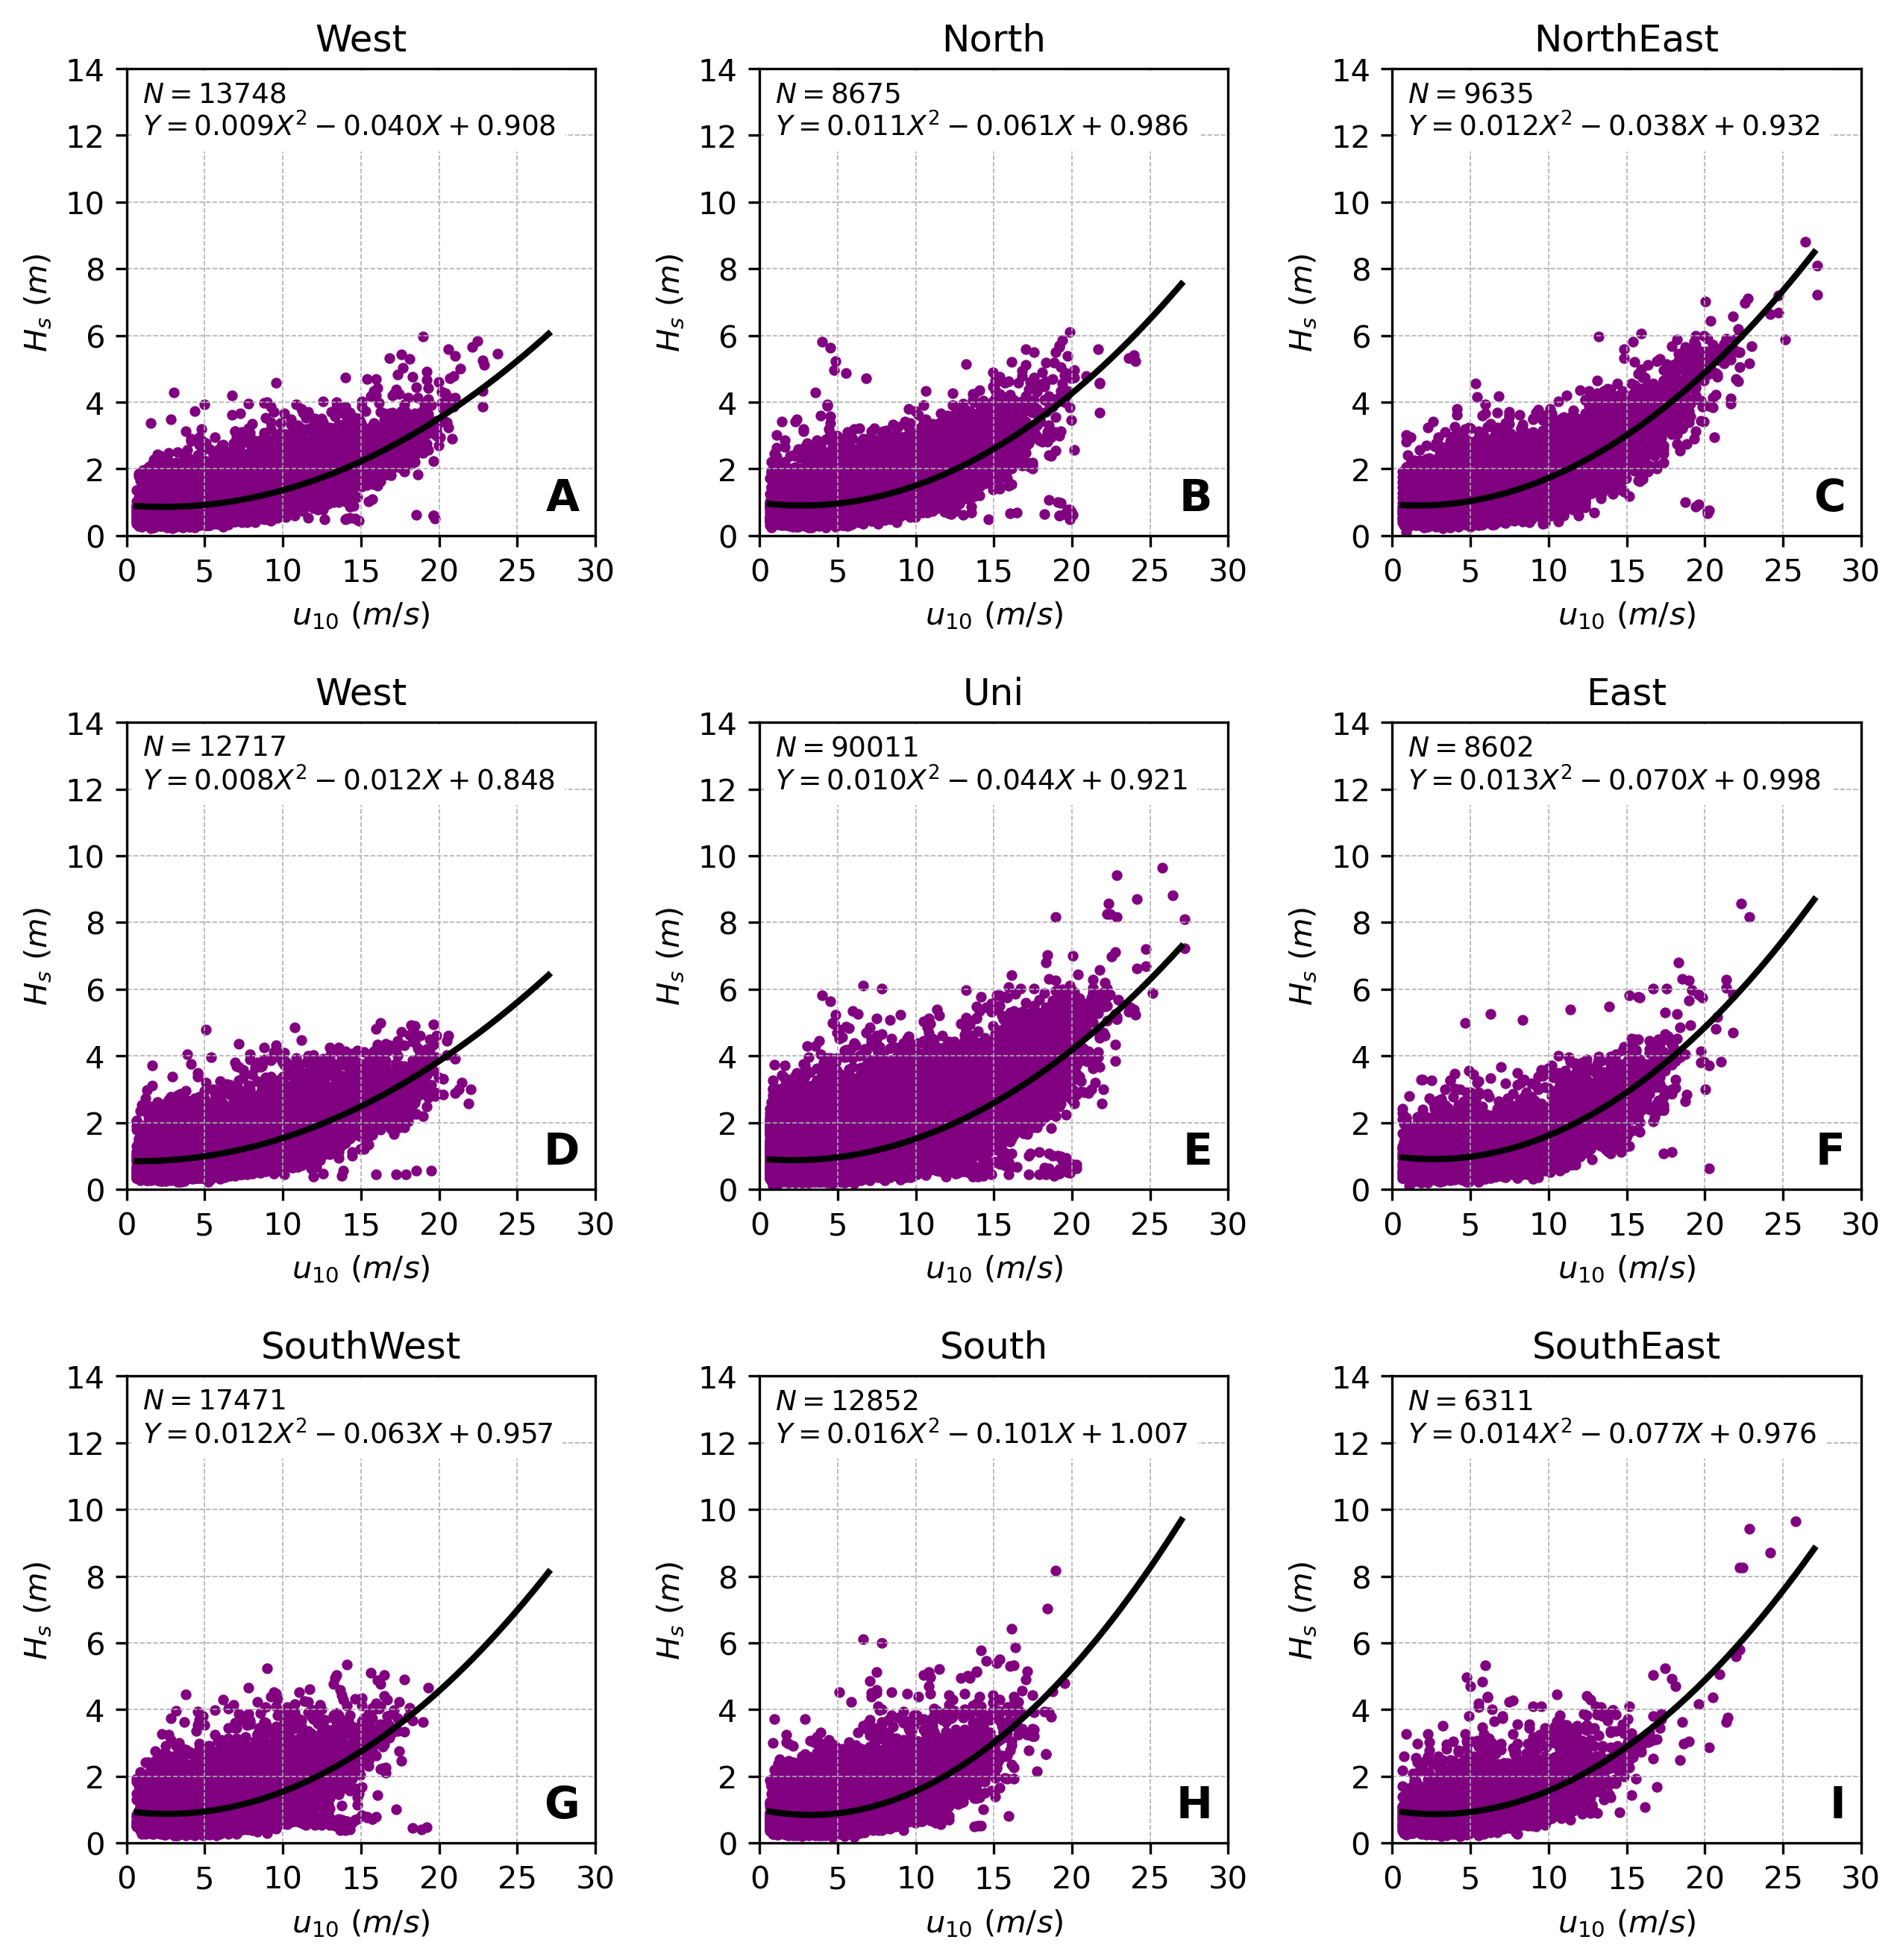
\includegraphics[width=0.95\linewidth]{Figures/Chapter5/b44025_wind_wave.png}
%\decoRule
\caption{Buoy 44025 wind wave relationships for each of the main wind directions and for all directions combined (E).}
\label{fig:wind_wave_44025}
\end{figure}


\begin{figure}[H]
\centering
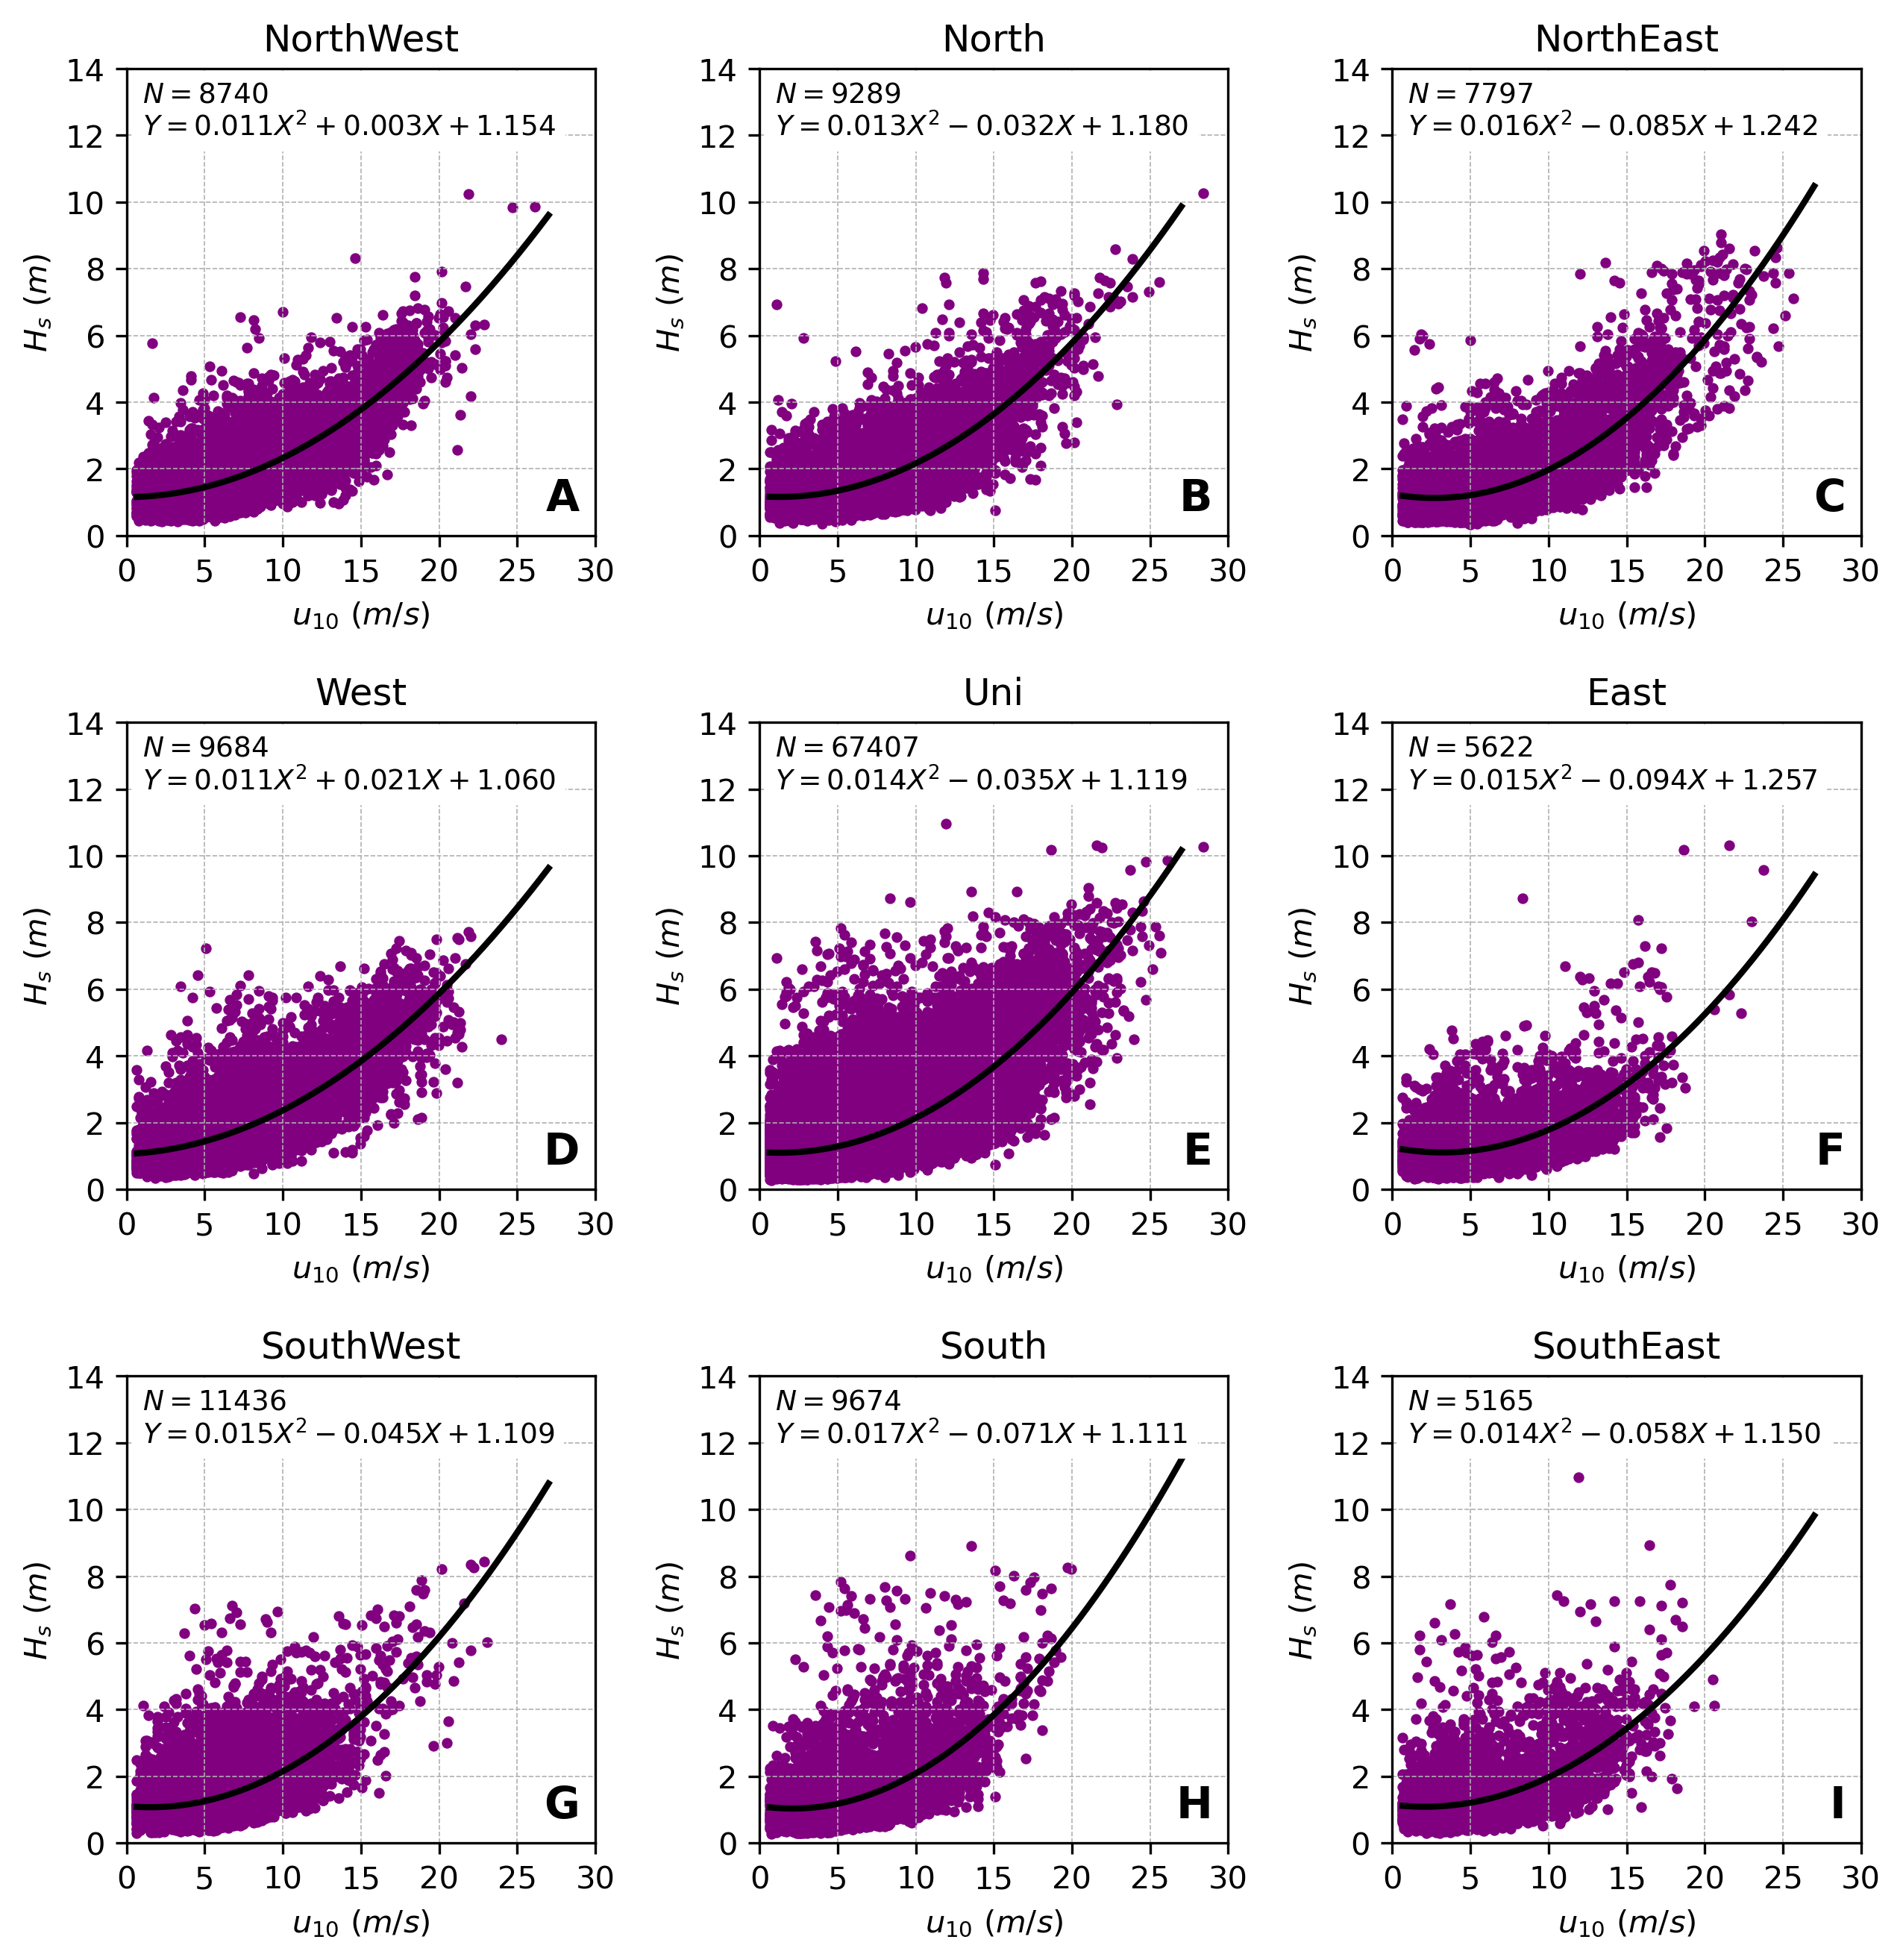
\includegraphics[width=0.95\linewidth]{Figures/Chapter5/b44008_wind_wave.png}
%\decoRule
\caption{Buoy 44008 wind wave relationships for each of the main wind directions and for all directions combined (E).}
\label{fig:wind_wave_44008}
\end{figure}


\begin{figure}[H]
\centering
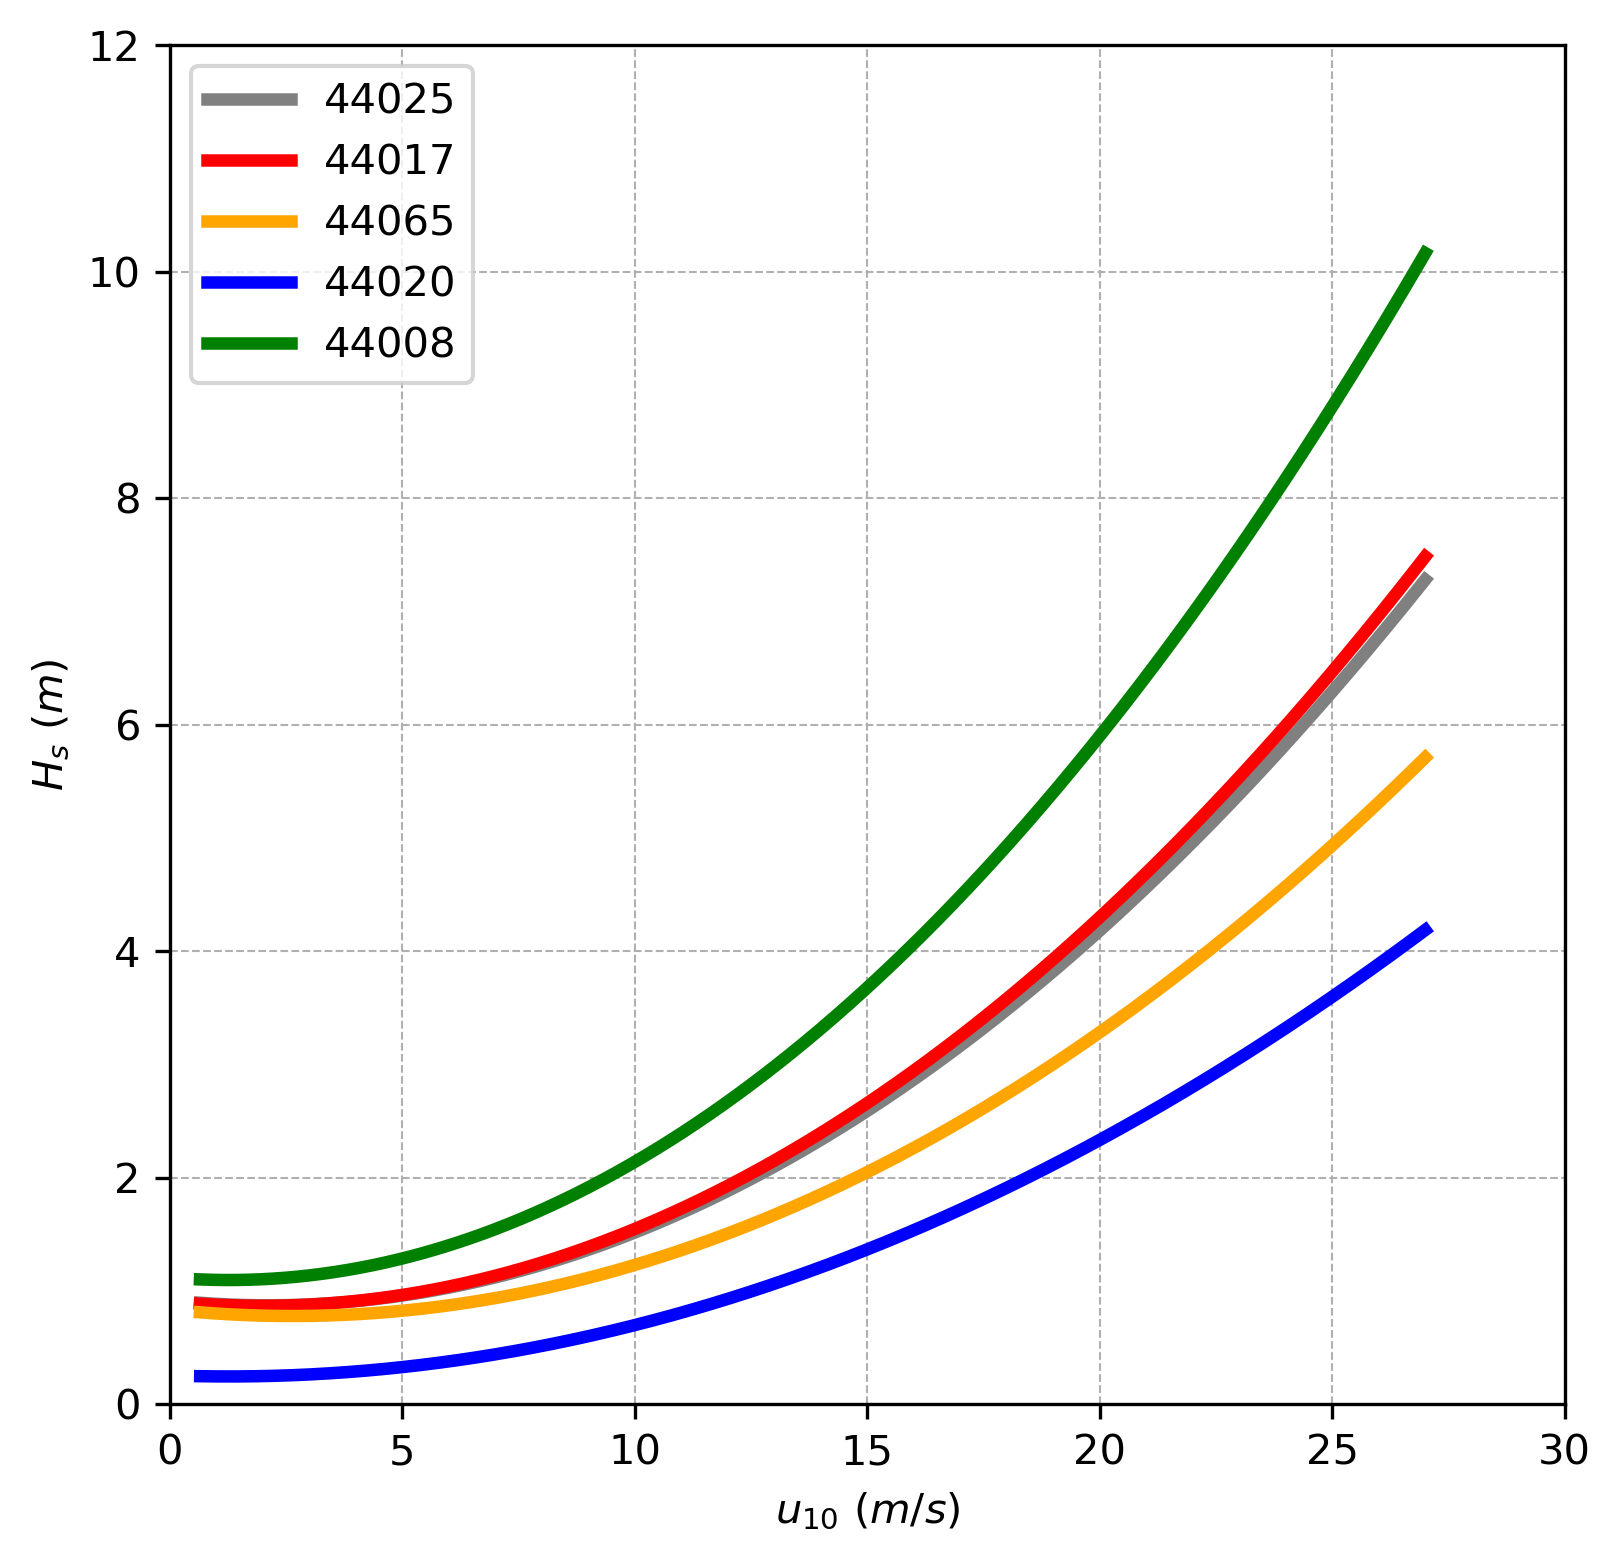
\includegraphics[width=0.8\linewidth]{Figures/Chapter5/wind_wave_5buoys.png}
%\decoRule
\caption{A comparison of the wind-wave relationships for the NDBC Buoys.}
\label{fig:wind_wave_buoys}
\end{figure}


\pagebreak


\section{Classification of ocean waves based on their inverse wave age}\label{inverse_wave_age}

The theoretical basis of the inverse wave age criterion is explained in \ref{decomposition_waveage}. The results presented in this section are based on the inverse wave age histograms for each buoy. Three figures are included: one for the whole datasets and two representing the inverse wave age distribution during the winter and summer seasons respectively. The estimated probabilities of occurrence for wind waves, mixed sea state, and swells are reported in Table~\ref{waveage_distribution}.



\begin{table}[H]
\begin{tabular*}{0.94\textwidth}{c@{\hskip 0.35in}cccccccccc @{\extracolsep{\fill}} cccccccccc}
\toprule
  \multirow{2}{0.4in}{\textbf{Buoy}} & \multicolumn{3}{c}{\textbf{Summer}} & \multicolumn{3}{c}{\textbf{Winter}} & \multicolumn{3}{c}{\textbf{All}} \\ 
    ~    & Wind   & Swell & Mixed & Wind   & Swell & Mixed & Wind & Swell & Mixed \\ \midrule
 44020 &        0.647 &         0.215 &         0.139 &        0.774 &         0.130 &         0.096 &  0.717 &  0.162 &  0.121 \\
 44065 &        0.129 &         0.483 &         0.387 &        0.382 &         0.444 &         0.173 &  0.247 &  0.474 &  0.279 \\
 44017 &        0.142 &         0.464 &         0.394 &        0.323 &         0.416 &         0.261 &  0.226 &  0.455 &  0.319 \\
 44025 &        0.149 &         0.457 &         0.393 &        0.446 &         0.354 &         0.201 &  0.284 &  0.413 &  0.302 \\
 44008 &        0.044 &         0.485 &         0.470 &        0.225 &         0.363 &         0.412 &  0.132 &  0.429 &  0.439 \\
 44066 &        0.163 &         0.424 &         0.413 &        0.433 &         0.290 &         0.276 &  0.280 &  0.368 &  0.352 \\ \bottomrule
\end{tabular*}
\caption {Frequency of occurence of wind-sea, swell and mixed sea state for NDBC buoys using the inverse wave age classification for winter, summer and all seasons.}
\label{waveage_distribution}
\end{table}


Generally, the inverse wave age distributions are bimodal. The first peak represents the mixed sea states and swells, and the second peak, the wind waves. The figures include a vertical dashed line that represents the wind-wave equilibrium. Sea states with an inverse wave over 0.83 are characterized as purely wind waves, although this is not a hard limit. Besides, an empirical limit for swell dominated sea states is an inverse wave age equal to 0.15. Waves with an inverse wave age between the two limits are categorized as mixed, and they are influenced both by wind-waves and swell. It is worth mentioning that the inverse wave age represents deep water waves at the peak, not the whole wave spectrum.


A general trend is that the second peak, which represents the wind waves, does not appear during the summer, except for the sheltered buoy 44020. The latter indicates again that swell's influence in this location is not significant with respect to the coastal and open ocean buoys. The bimodal distribution retains its characteristics during the summer with higher wind waves and lower probability of mixed/swell waves. During winter, almost 80\% of the waves are purely influenced by the wind in this location. This result is connected with the low WS seasonal variability in Figure~\ref{fig:buoy_wave_seasonality}B. The above does not apply to the coastal buoys and the open ocean buoy 44066. Figures \ref{fig:inv_wave_age_buoys_winter}B,C,D,F show clear peaks after the wind-wave equilibrium during the winter, when the influence of the wind is most substantial due to the high values of $u_{10}$. However, the second peak ceases to appear during the summer distributions in Figure~\ref{fig:inv_wave_age_buoys_summer}, and at the same time, the mixed/swell probability density peaks almost double their value. The western part of the region is significantly influenced by the wind, especially during winter, when the wind-waves' probability is nearly as high as the probability of swell/mixed seas. For buoy 44025, purely wind waves are developing three times less during the summer than the winter, when the probability density peak is higher than the swell/mixed.


For the open ocean buoy 44008, the inverse wave age distribution appears to have a single peak throughout the year. During the winter, this peak has a lower probability density, and the distribution is more spread to a broader range of inverse wave age values. In contrast, over 95\% of the waves are characterized as mixed or swell based on the inverse wave age classification during summer. Consequently, the wind waves' influence during the summer is minimal for the eastern part of SNE and at a distance over 100 kilometers from the closest coast. 




\begin{figure}[H]
\centering
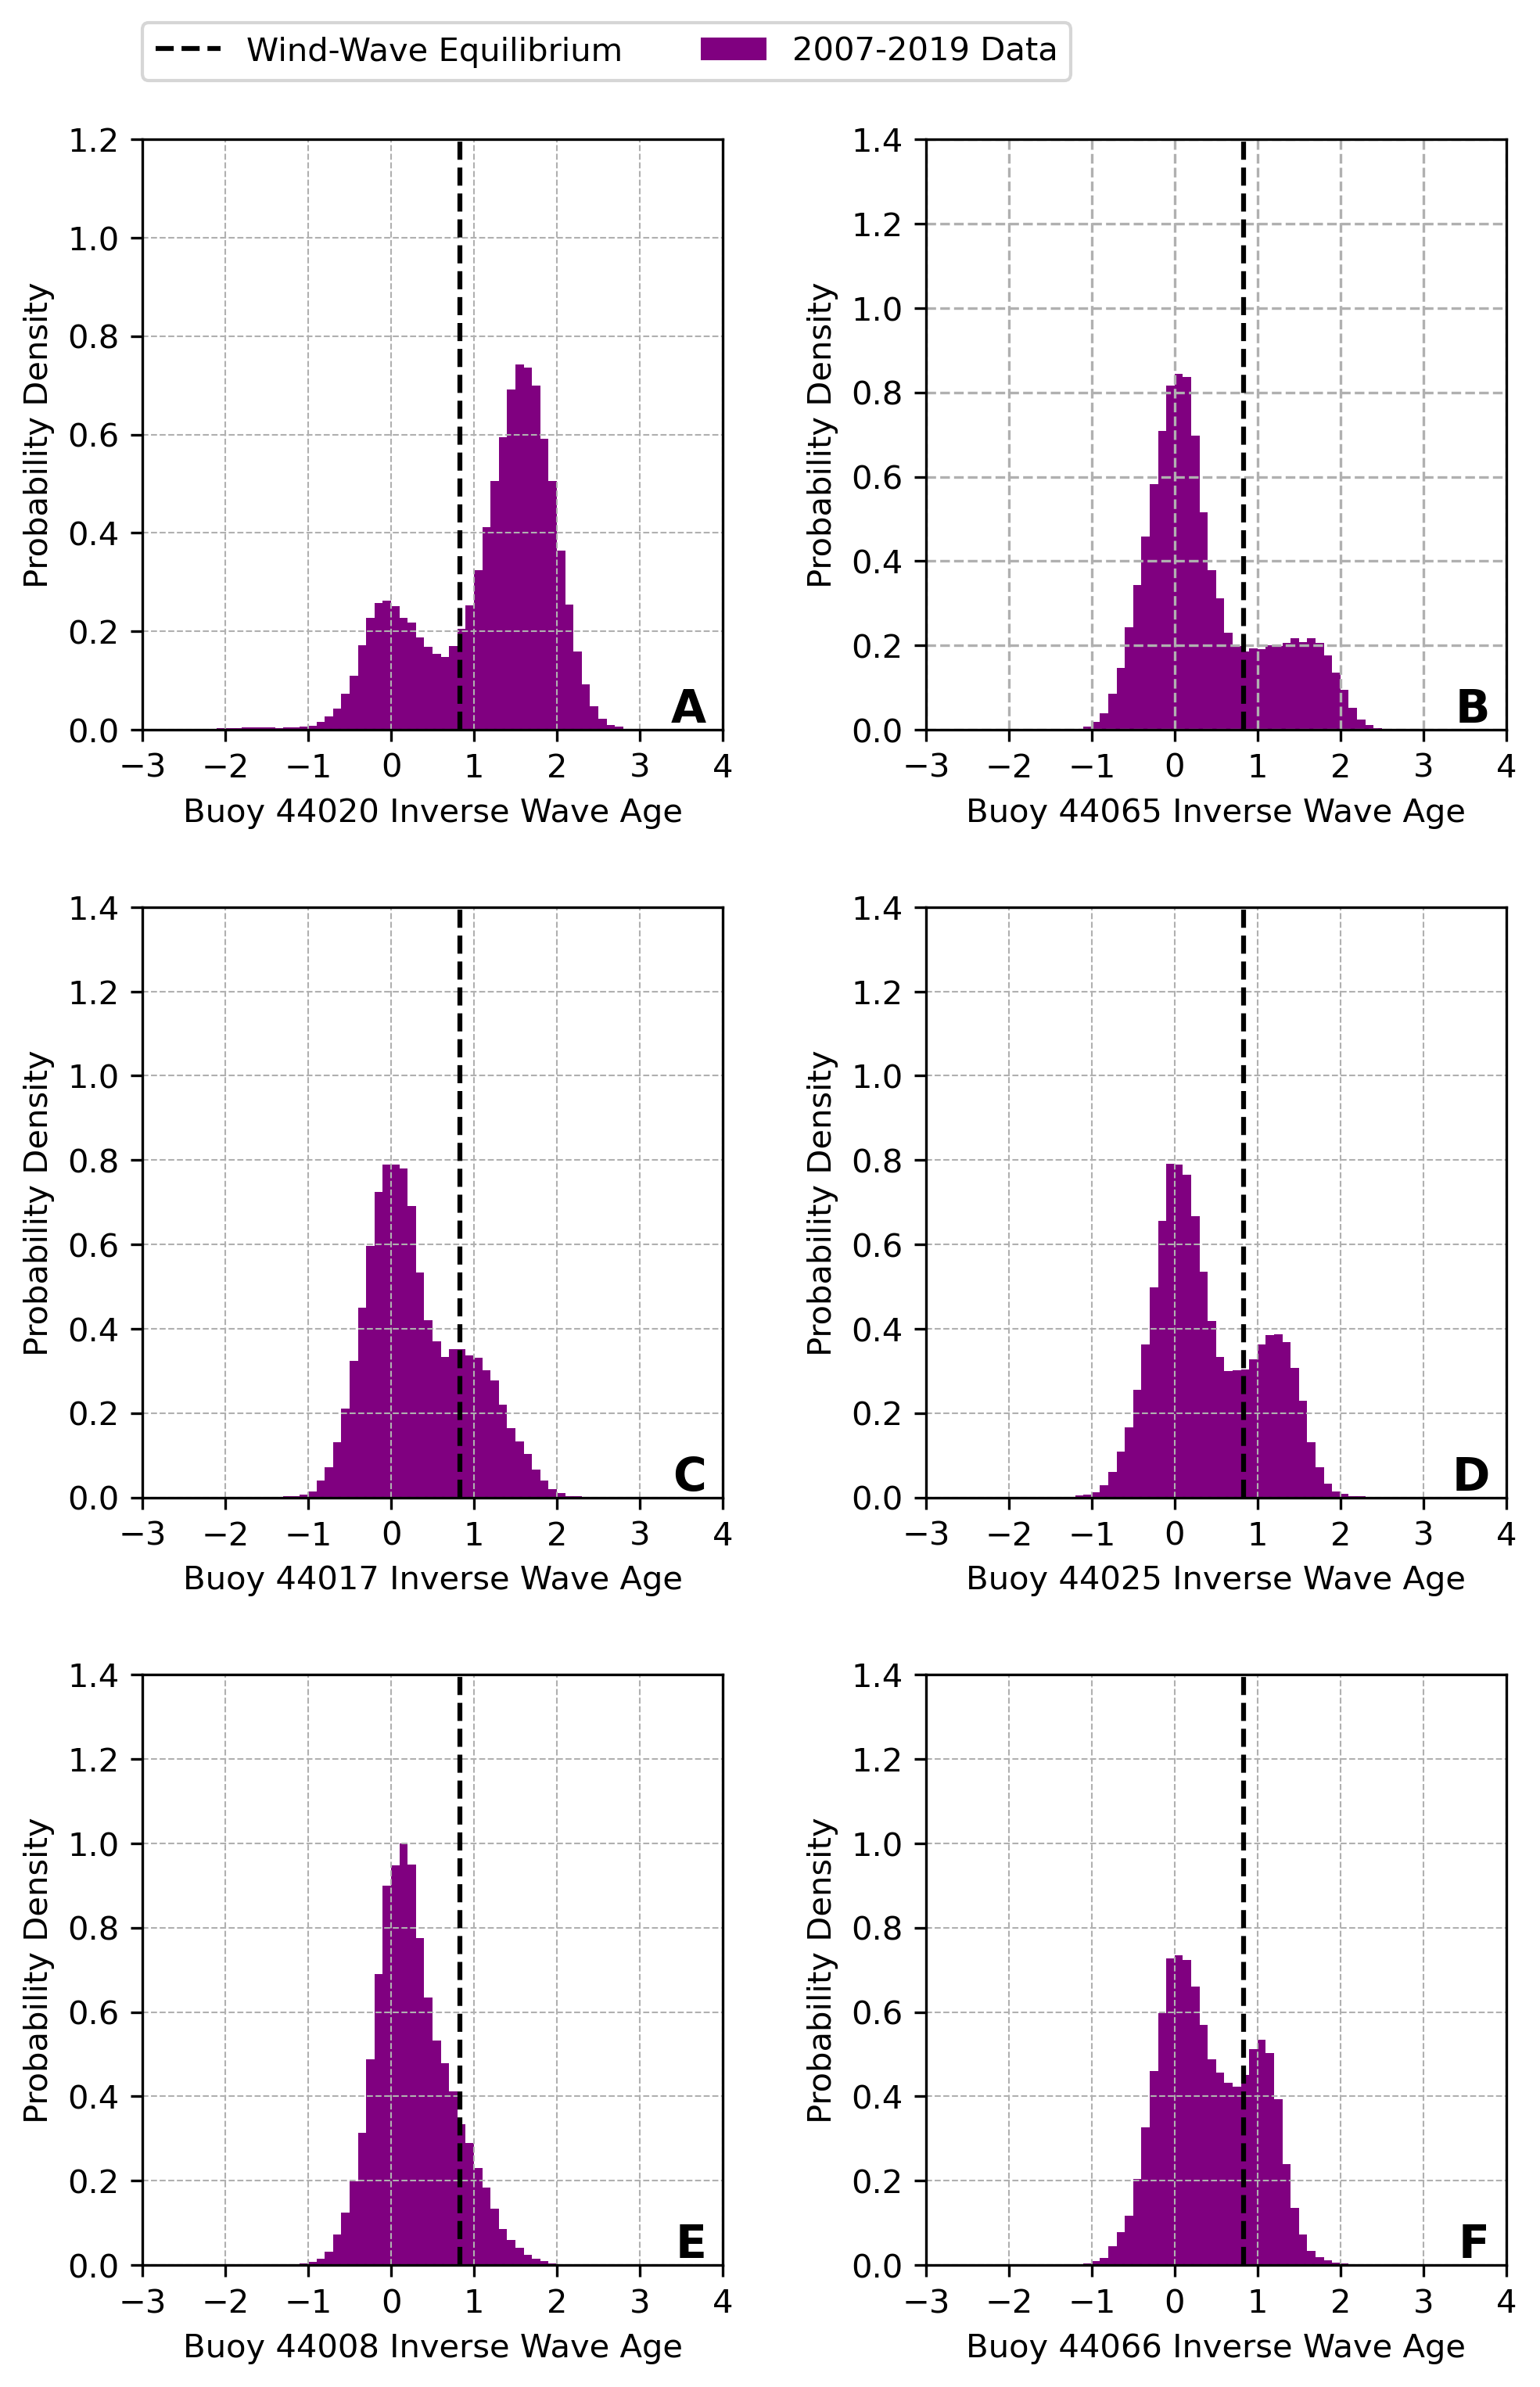
\includegraphics[width=0.95\linewidth]{Figures/Chapter5/inv_wave_age_pdfs.png}
%\decoRule
\caption{NDBC buoys Inverse Wave Age distribution.}
\label{fig:inv_wave_age_buoys}
\end{figure}


\begin{figure}[H]
\centering
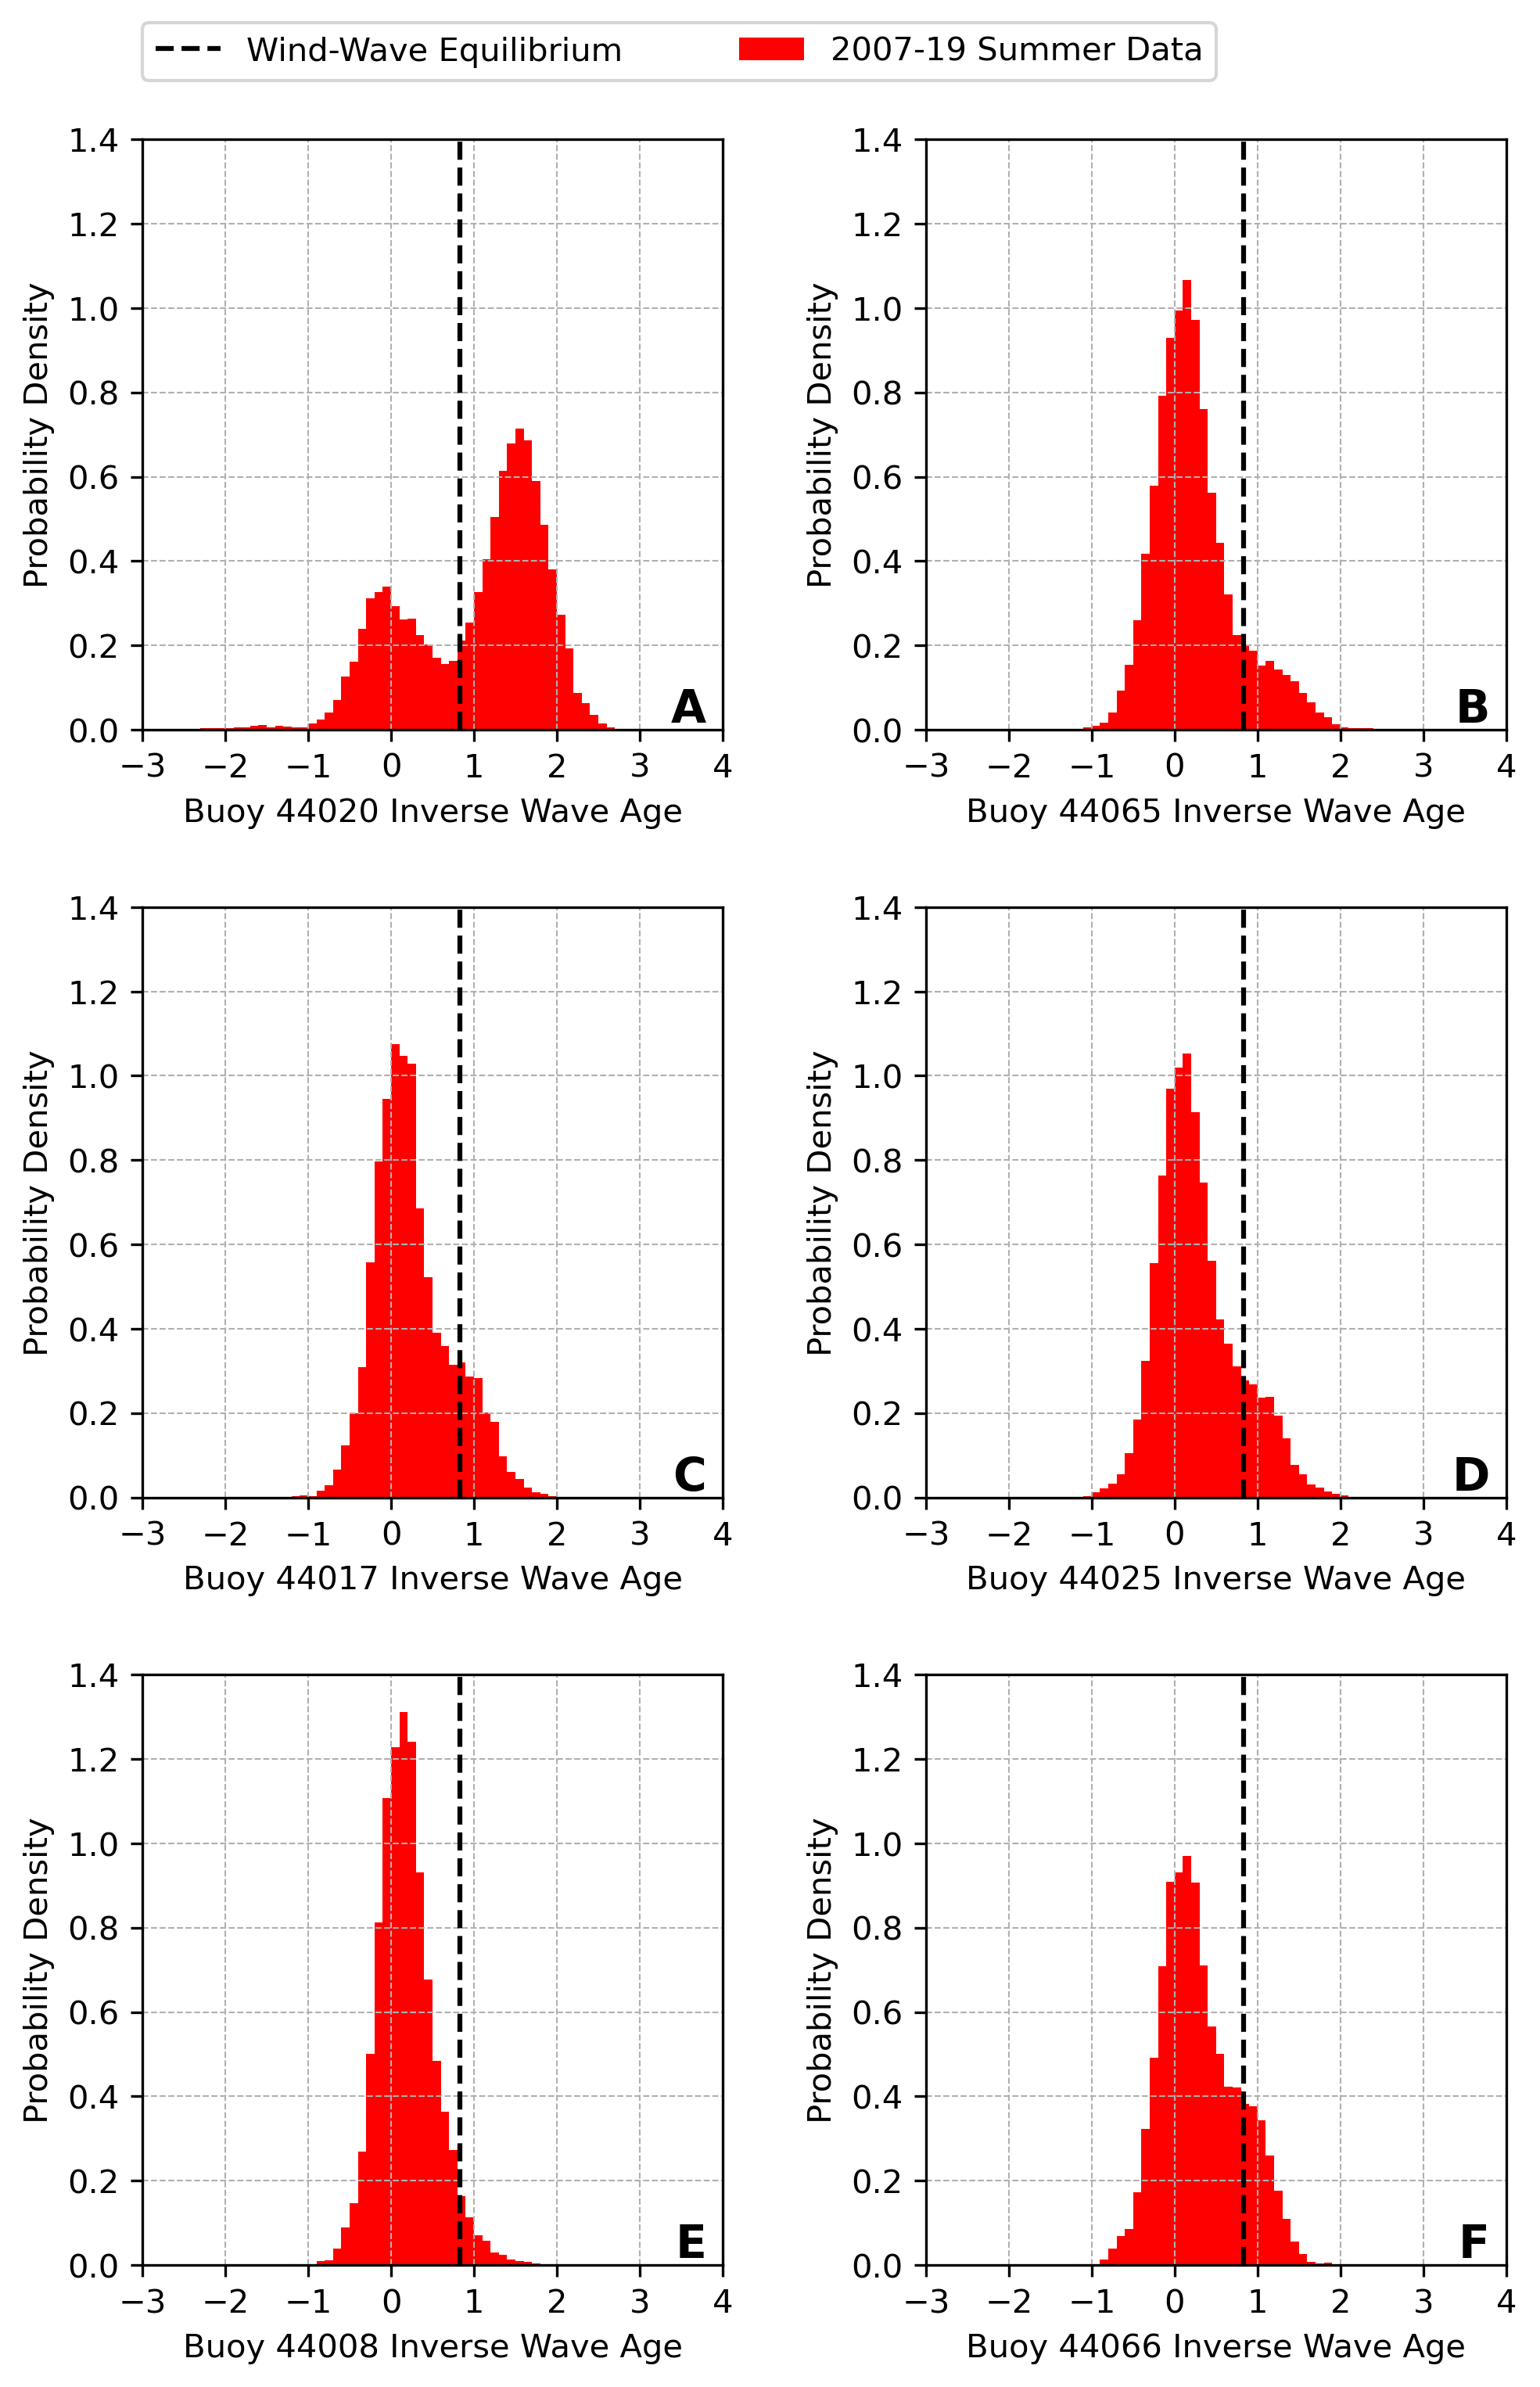
\includegraphics[width=0.95\linewidth]{Figures/Chapter5/inv_wave_age_pdfs_summer.png}
%\decoRule
\caption{NDBC buoys summer Inverse Wave Age distribution.}
\label{fig:inv_wave_age_buoys_summer}
\end{figure}


\begin{figure}[H]
\centering
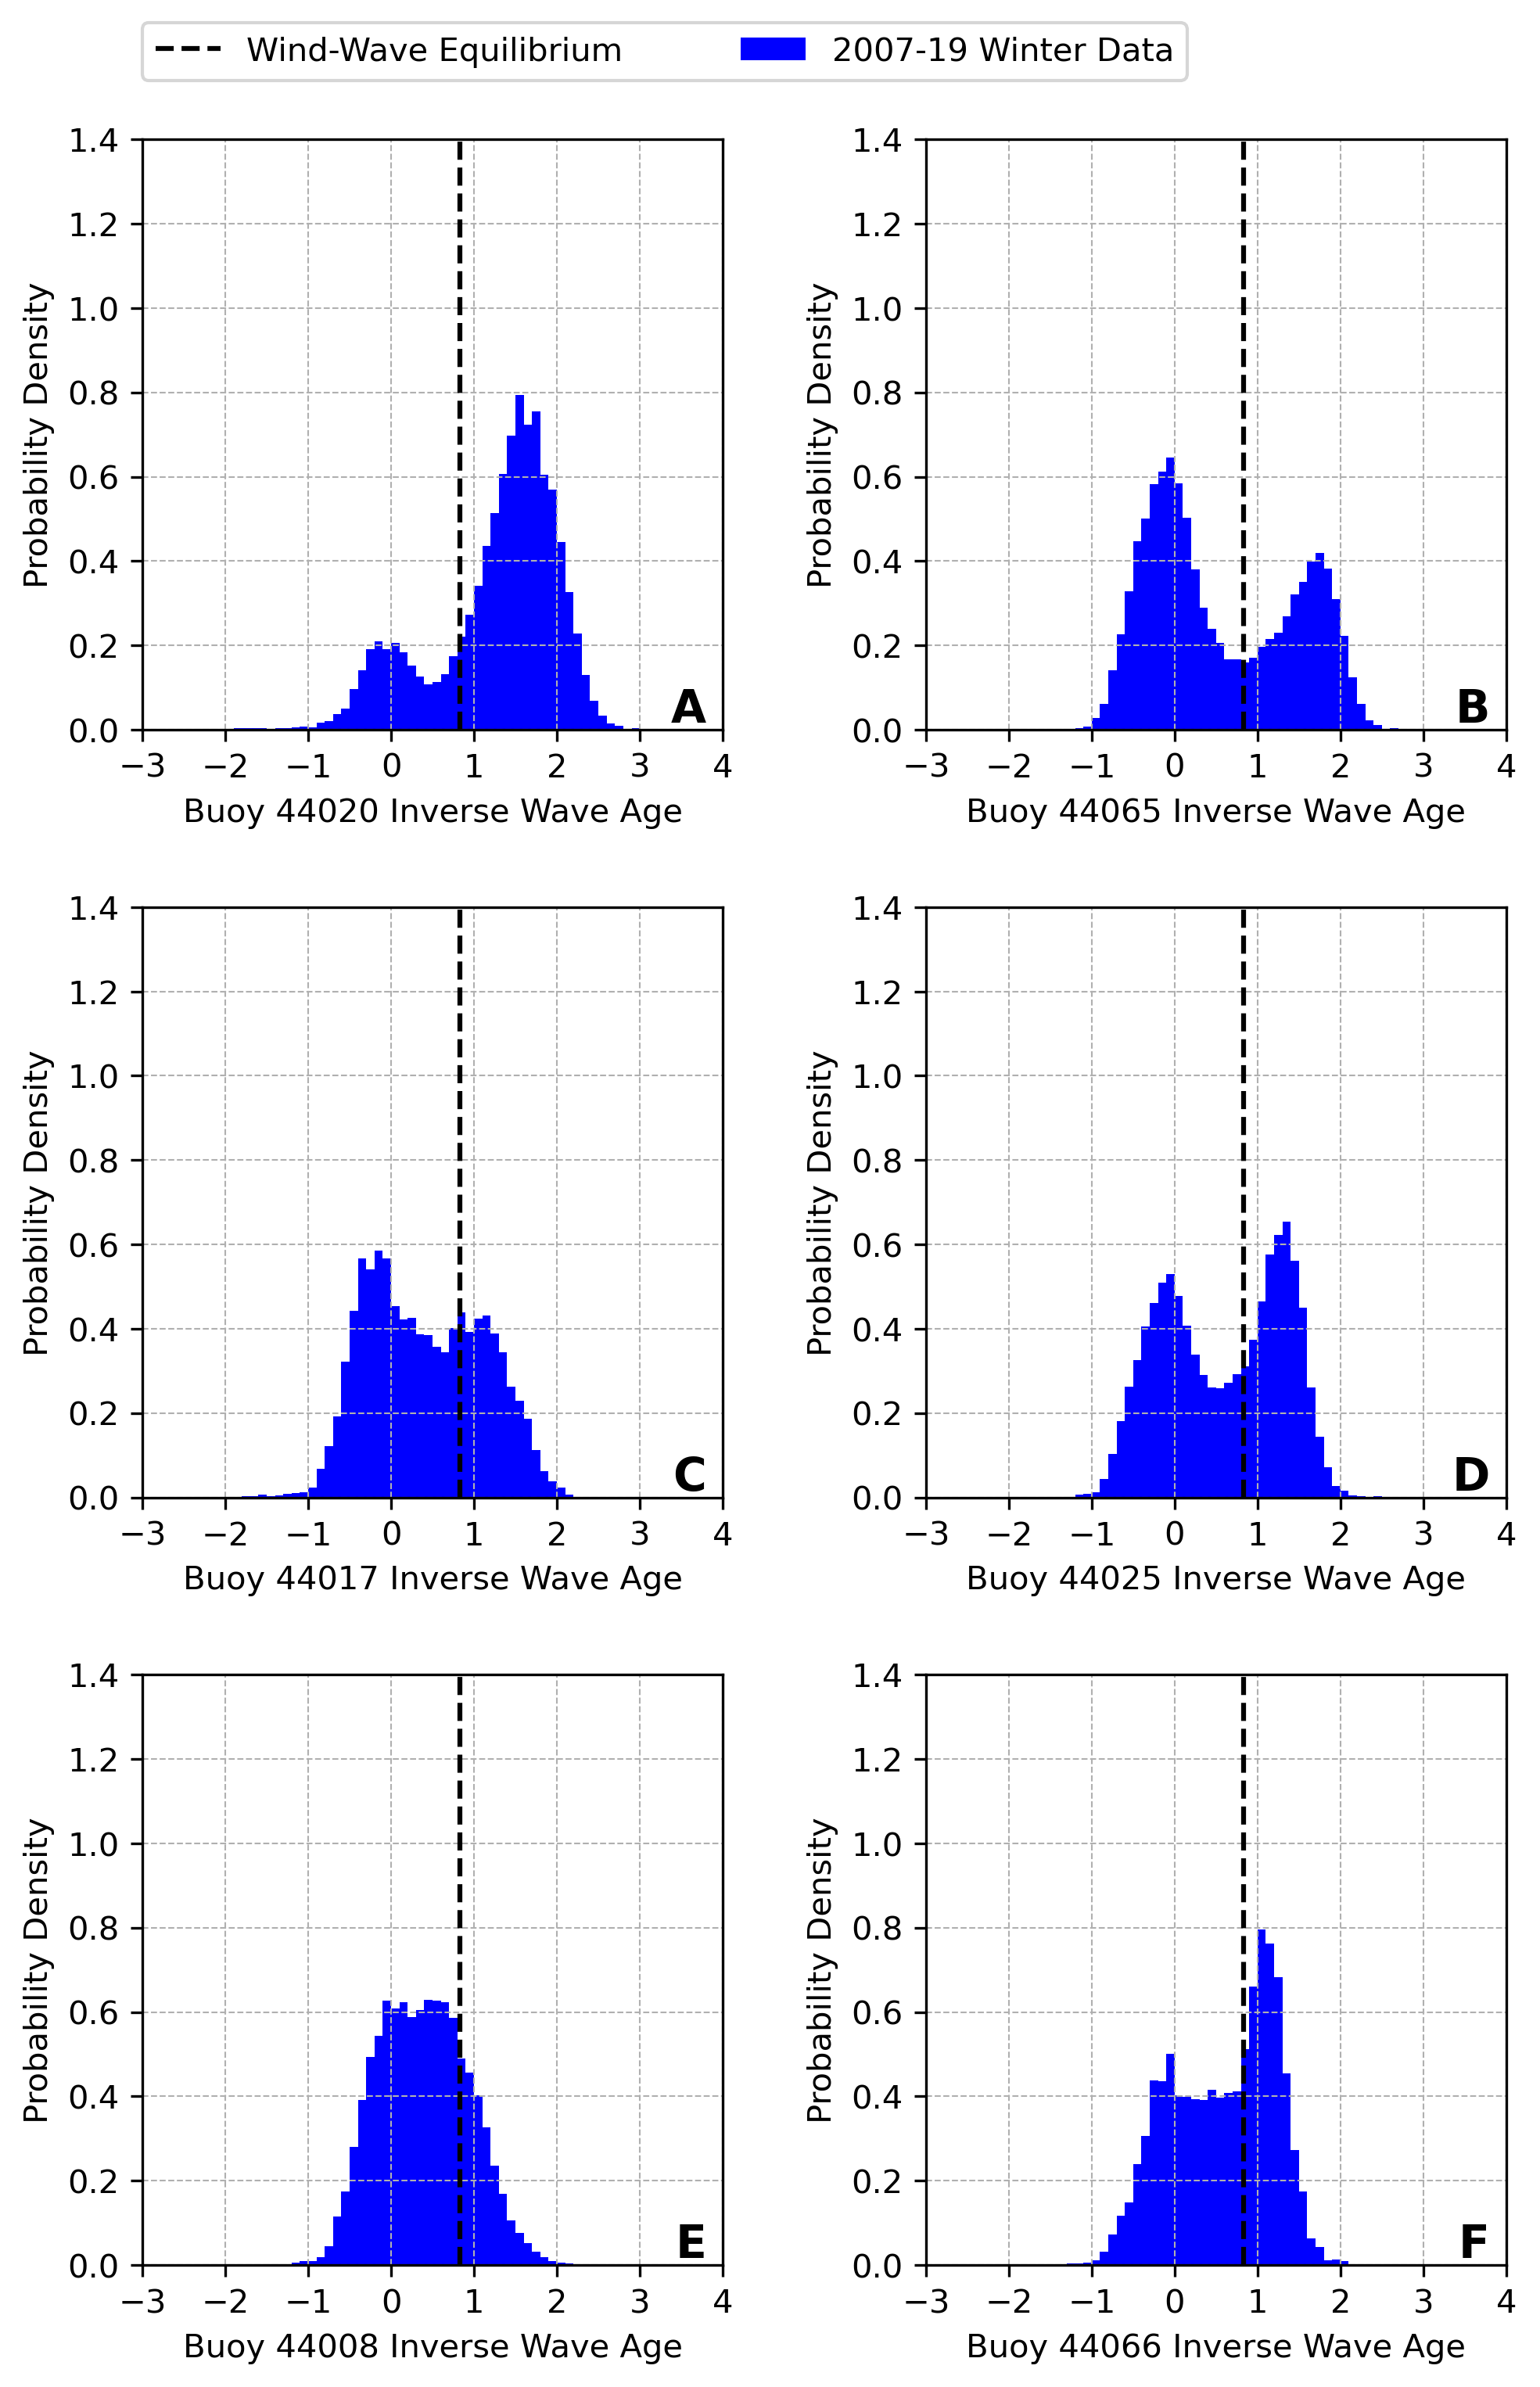
\includegraphics[width=0.95\linewidth]{Figures/Chapter5/inv_wave_age_pdfs_winter.png}
%\decoRule
\caption{NDBC buoys winter Inverse Wave Age distribution.}
\label{fig:inv_wave_age_buoys_winter}
\end{figure}

%-------------------------------------------------------------------------------------------

\section{A case study of extreme events}\label{extreme_event}

In the previous sections, the focus was on the normal wind-wave conditions. On the other hand, extreme winds and waves are often described by values at the upper tail of the $u_{10}$ and $H_{s}$ probability density functions. The study of extreme events is essential and precedes the offshore wind farms' design and construction to assess the wind turbine fatigue loads.
This section aims to describe the wind and wave mechanisms underlying the development of the most frequent extreme events in SNE, the extratropical storms, or Nor'easters, defined in \ref{study_area}. 


\begin{figure}[H]
\centering
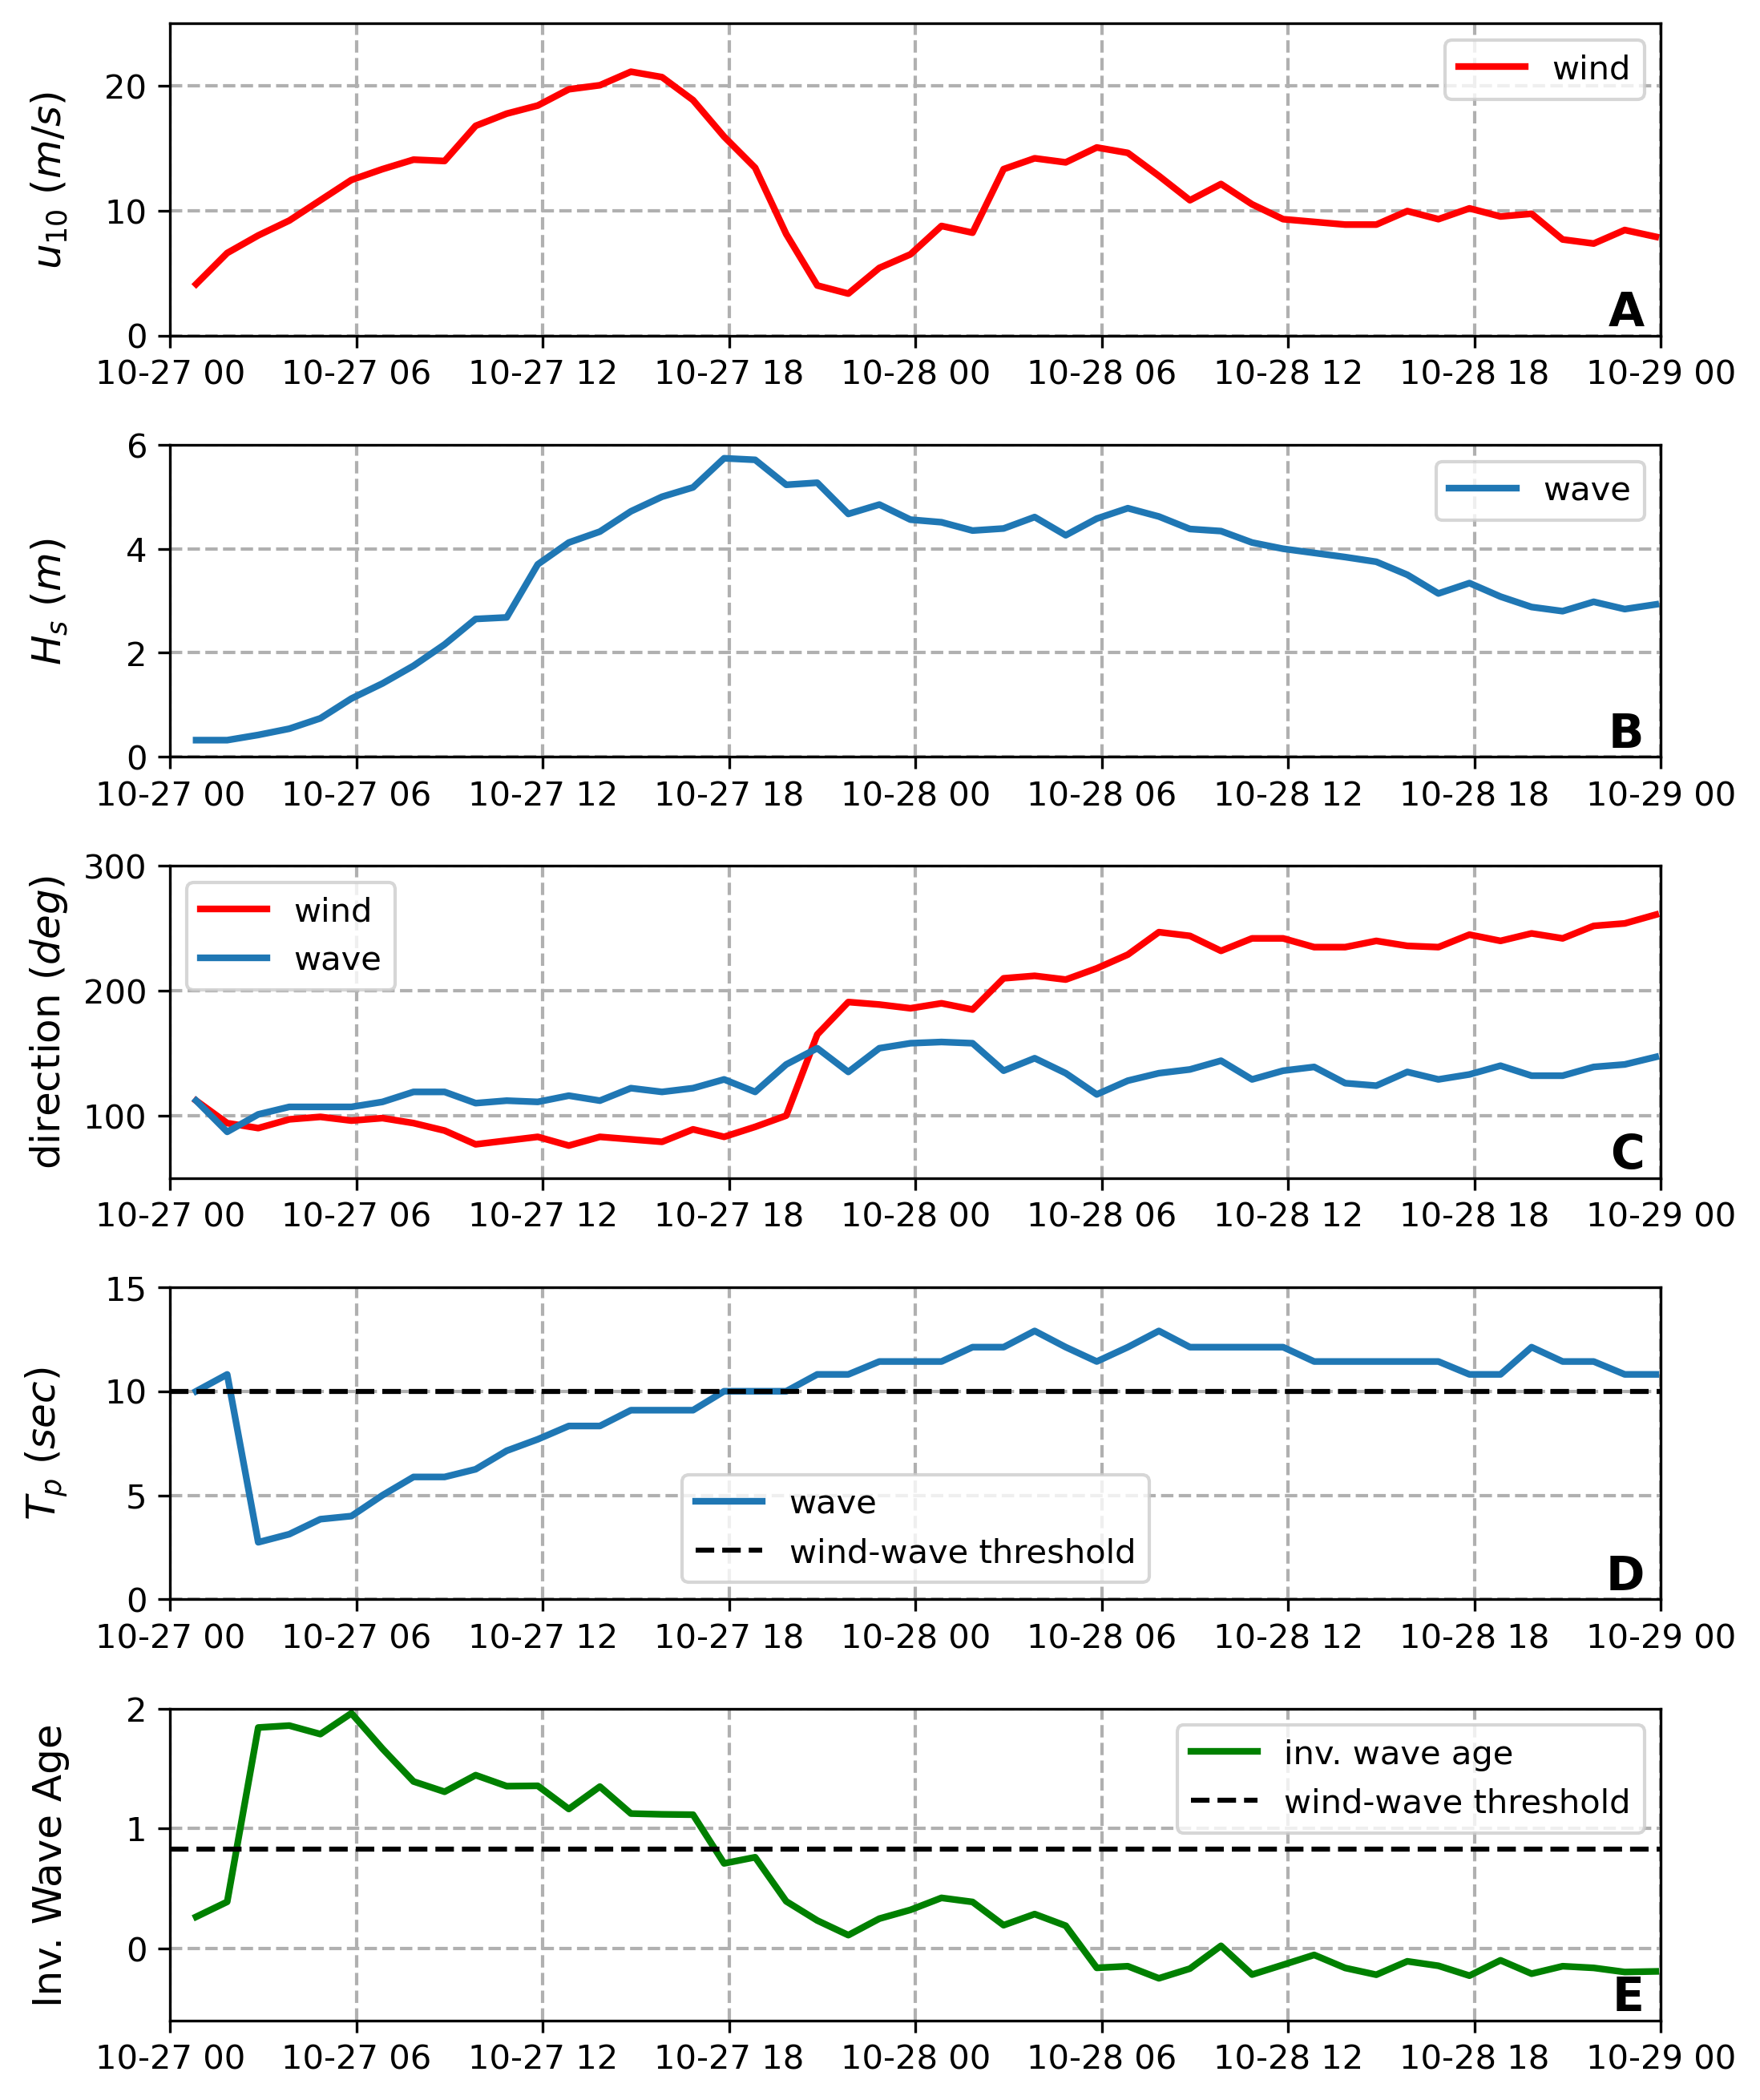
\includegraphics[width=0.75\linewidth]{Figures/Chapter5/noreaster_oct18_3days.png}
%\decoRule
\caption{Time series of the main wind and wave parameters measured by buoy 44017 during October 27 and 28, 2018 describing the passing of the Nor'easter.}
\label{fig:noreaster_oct18_ts}
\end{figure}


The time series of the wind and wave parameters measured by buoy 44017 in Figure~\ref{fig:noreaster_oct18_ts} shows the development of the Nor'easter storm that passed from SNE on October 27, 2018, bringing extreme waves and coastal flooding. In the early morning hours of October 27, light winds and calm sea states are present before the storm's passing. Wind and waves are coming from the same, east-southeast direction. As the wind increases its intensity, the waves' $H_{s}$ and $T_{p}$ also progressively increase. The WS reaches its maximum at around 3:00 PM, while the sea state becomes roughest with a three-hour lag at 6:00 PM. 


\begin{figure}[H]
\centering
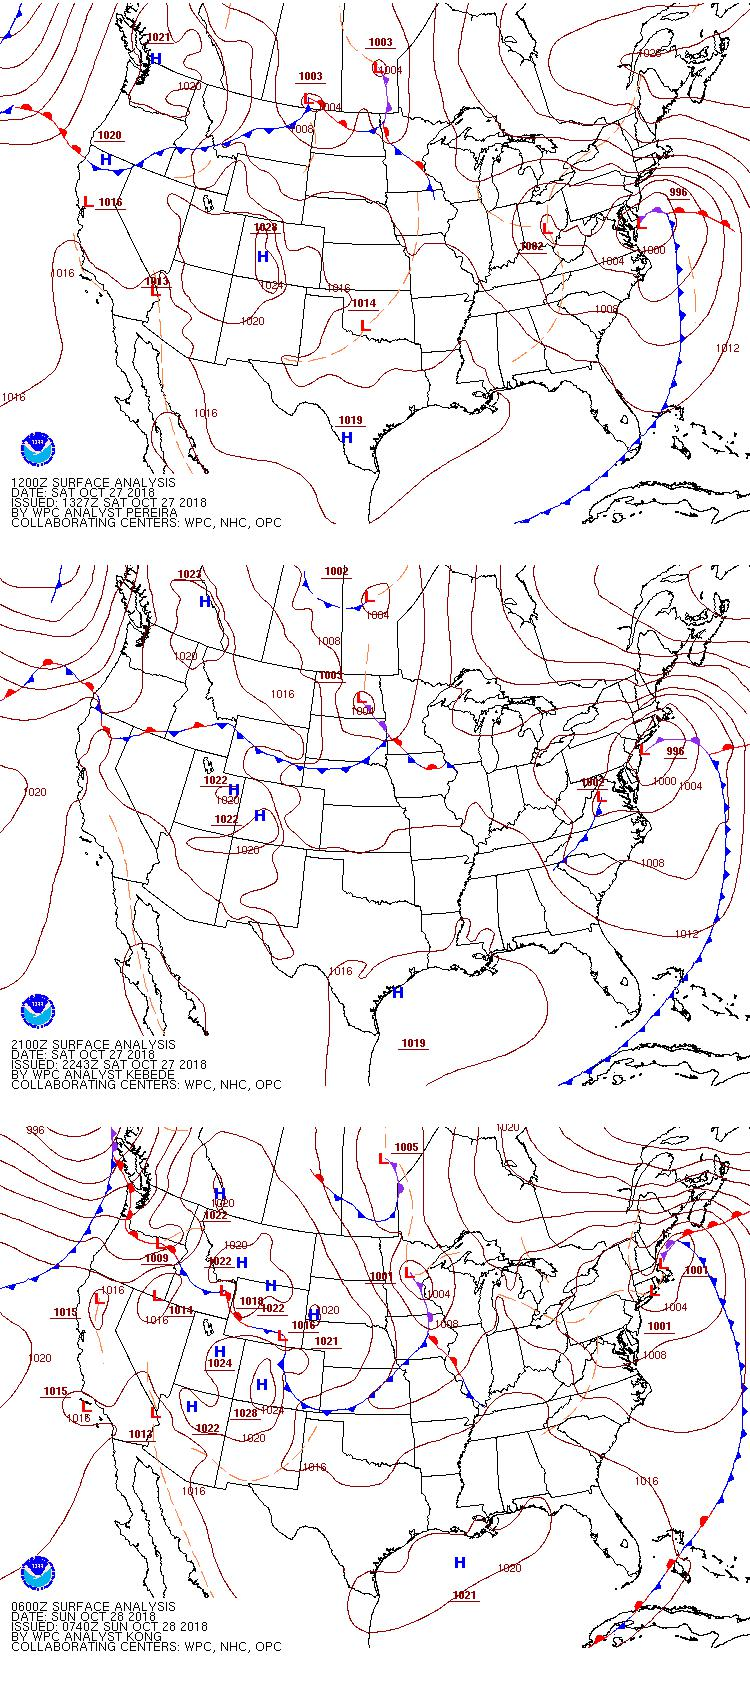
\includegraphics[width=0.7\linewidth]{Figures/Chapter5/noreaster_oct18_sa.jpg}
%\decoRule
\caption{Surface analysis maps before (upper panel), during (center panel) and after (bottom panel) the passing of the October 27, 2018 Nor'easter from SNE. Derived from: \href{https://www.wpc.ncep.noaa.gov/archives/web_pages/sfc/sfc_archive.php}{WPC's Surface Analysis Archive}}.
\label{fig:noreaster_oct18_sa}
\end{figure}



\begin{figure}[H]
\centering
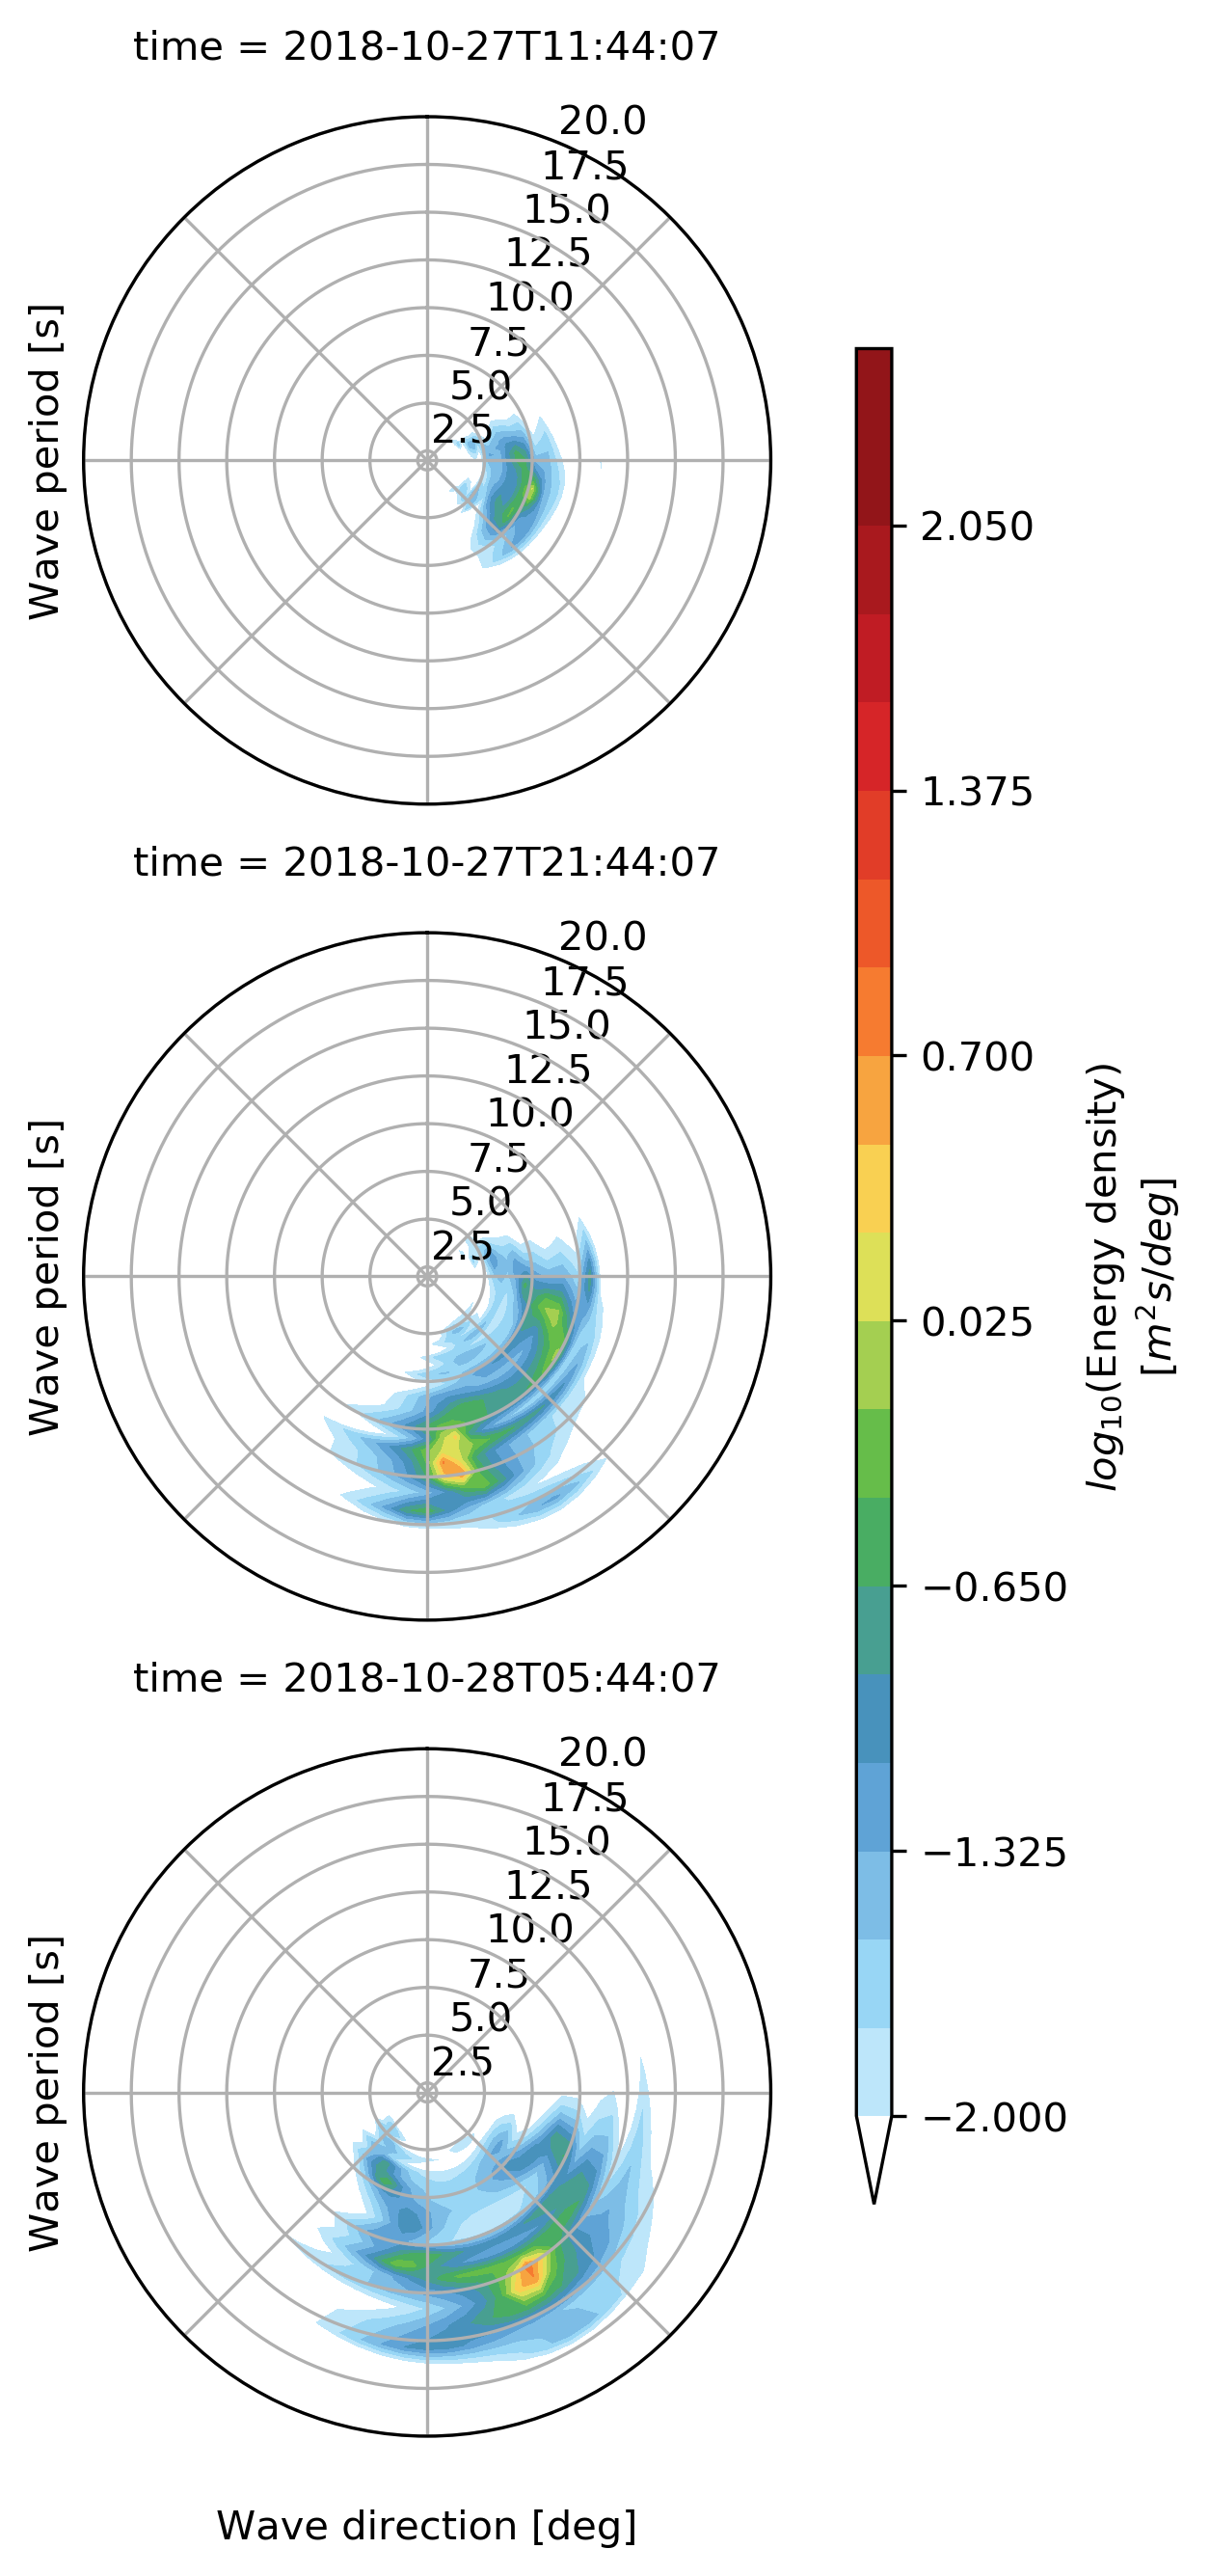
\includegraphics[width=0.5\linewidth]{Figures/Chapter5/noreaster_oct18_snap.png}
%\decoRule
\caption{Buoy 44097 directional wave spectra before (upper figure), during (center figure) and after (bottom figure) the passing of the October 27, 20018 Nor'easter over SNE. Values represent the energy density logarithm for better visualization.}
\label{fig:noreaster_oct18_snap}
\end{figure}


At 6:00 PM, the wind also starts to shift its direction to the south while the wind intensity decreases to a minimum at 9:00 PM. The combination of the WS decrease and the shift of the wind's direction is critical for developing a local south-southwestern swell system. From this point on, wind and waves are coming from different directions. Considering the dominant period, it passes the crude 10-seconds wind-wave threshold simultaneously to the WS's minimum. If we also look at the inverse wave age time series, the sea state becomes mixed at the same time when the SWH peak occurs and becomes swell-dominated between 5:00 to 6:00 AM of October 28. The wind, which started to increase again on October 27 at 9:00 PM, reaches a second but lower maximum and remains almost constant from the early hours of October 28 and throughout the day. The waves remain substantially high (over 4 meters) until noon on October 28, but they are gradually losing their energy.


\begin{figure}[H]
\centering
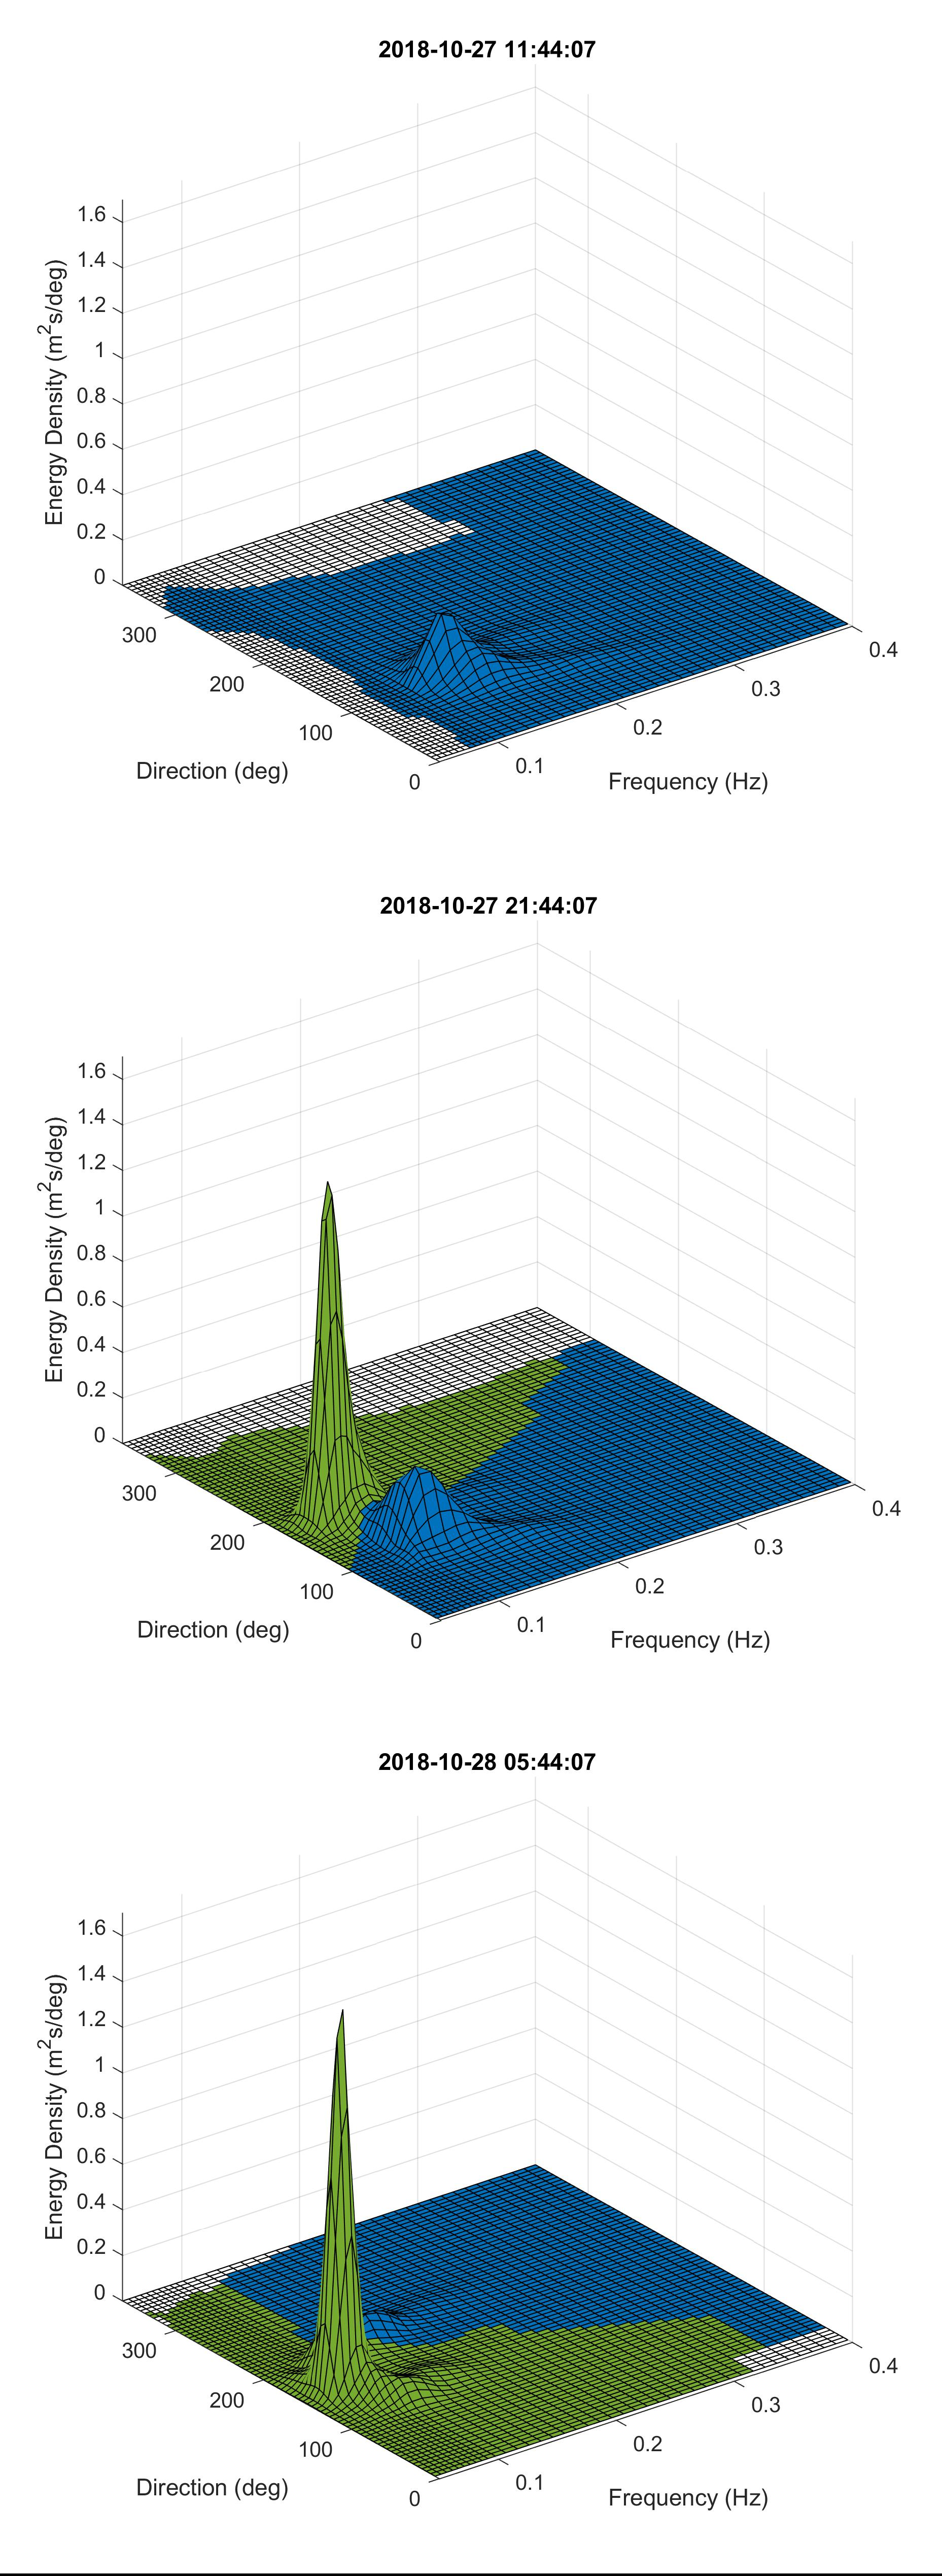
\includegraphics[width=0.58\linewidth]{Figures/Chapter5/noreaster_oct18_ds.jpg}
%\decoRule
\caption{Spectral partitioning of the buoy 44097 directional wave spectra before (upper figure), during (center figure) and after (bottom figure) the passing of the October 27, 2018 Nor'easter over SNE.}
\label{fig:noreaster_oct18_ds}
\end{figure}


Figure~\ref{fig:noreaster_oct18_sa} includes the surface analysis maps from the Weather Prediction Center's (WPC) archive before, during, and after the passing of the Nor'easter from SNE. For a more detailed analysis, we provide the buoy 44097 directional spectra. Figure~\ref{fig:noreaster_oct18_snap} includes three snapshots of the storm development based on buoy observations, almost coinciding with the surface analysis maps. The upper figure at 11:44 AM shows a single wind-wave system with relatively small but increasing elevation variance density and a dominant period of 7-8 seconds. After the wind direction shift at 9:44 PM,  we can distinguish the split in two separate systems, the wind-wave, and the south-southeast swell, with an 11 to 12 seconds period. After nine hours, only the swell system is still present. Figure~\ref{fig:noreaster_oct18_ds} is an even more realistic representation of the sea state and the result of spectral partitioning of the aforementioned directional spectra described in \ref{decomposition_waveage}. The blue color represents wind-waves, green is for the first swell system, and the noise, the spectral domain where zero energy is observed, is the white part of the directional wave spectra. In the upper figure, the wind-wave system with low elevation variance density is only observed. At 9:44 PM, the swell system has already been generated by the shift in the wind direction, and we can identify the two separated peaks. This snapshot is an example of a mixed sea state when the highest peak represents the swell and the lowest the wind-wave. The latter gradually loses its energy, and in the early morning hours of October 28 (lower figure), the swell system is dominant but with decreased elevation variance density.


\pagebreak

%------------------------------------------------------------------------
-------------------


\section{Validation of Altimeter WS and SWH observations in the SNE region}\label{validation_SNE}


A description of the inherent challenges of validating satellite altimeter observations with ground truth stations is available in Section~\ref{collocation}. Sensors onboard buoys and altimeters are sensitive to errors. However, even if we considered their measurements perfect, deviations would still exist on the match-up observations due to the spatial and temporal sampling and representation differences based on each measurement system's principles. The results presented in this section aim to quantify how well altimeters match buoy observations on a regional level. 


\begin{figure}[H]
\centering
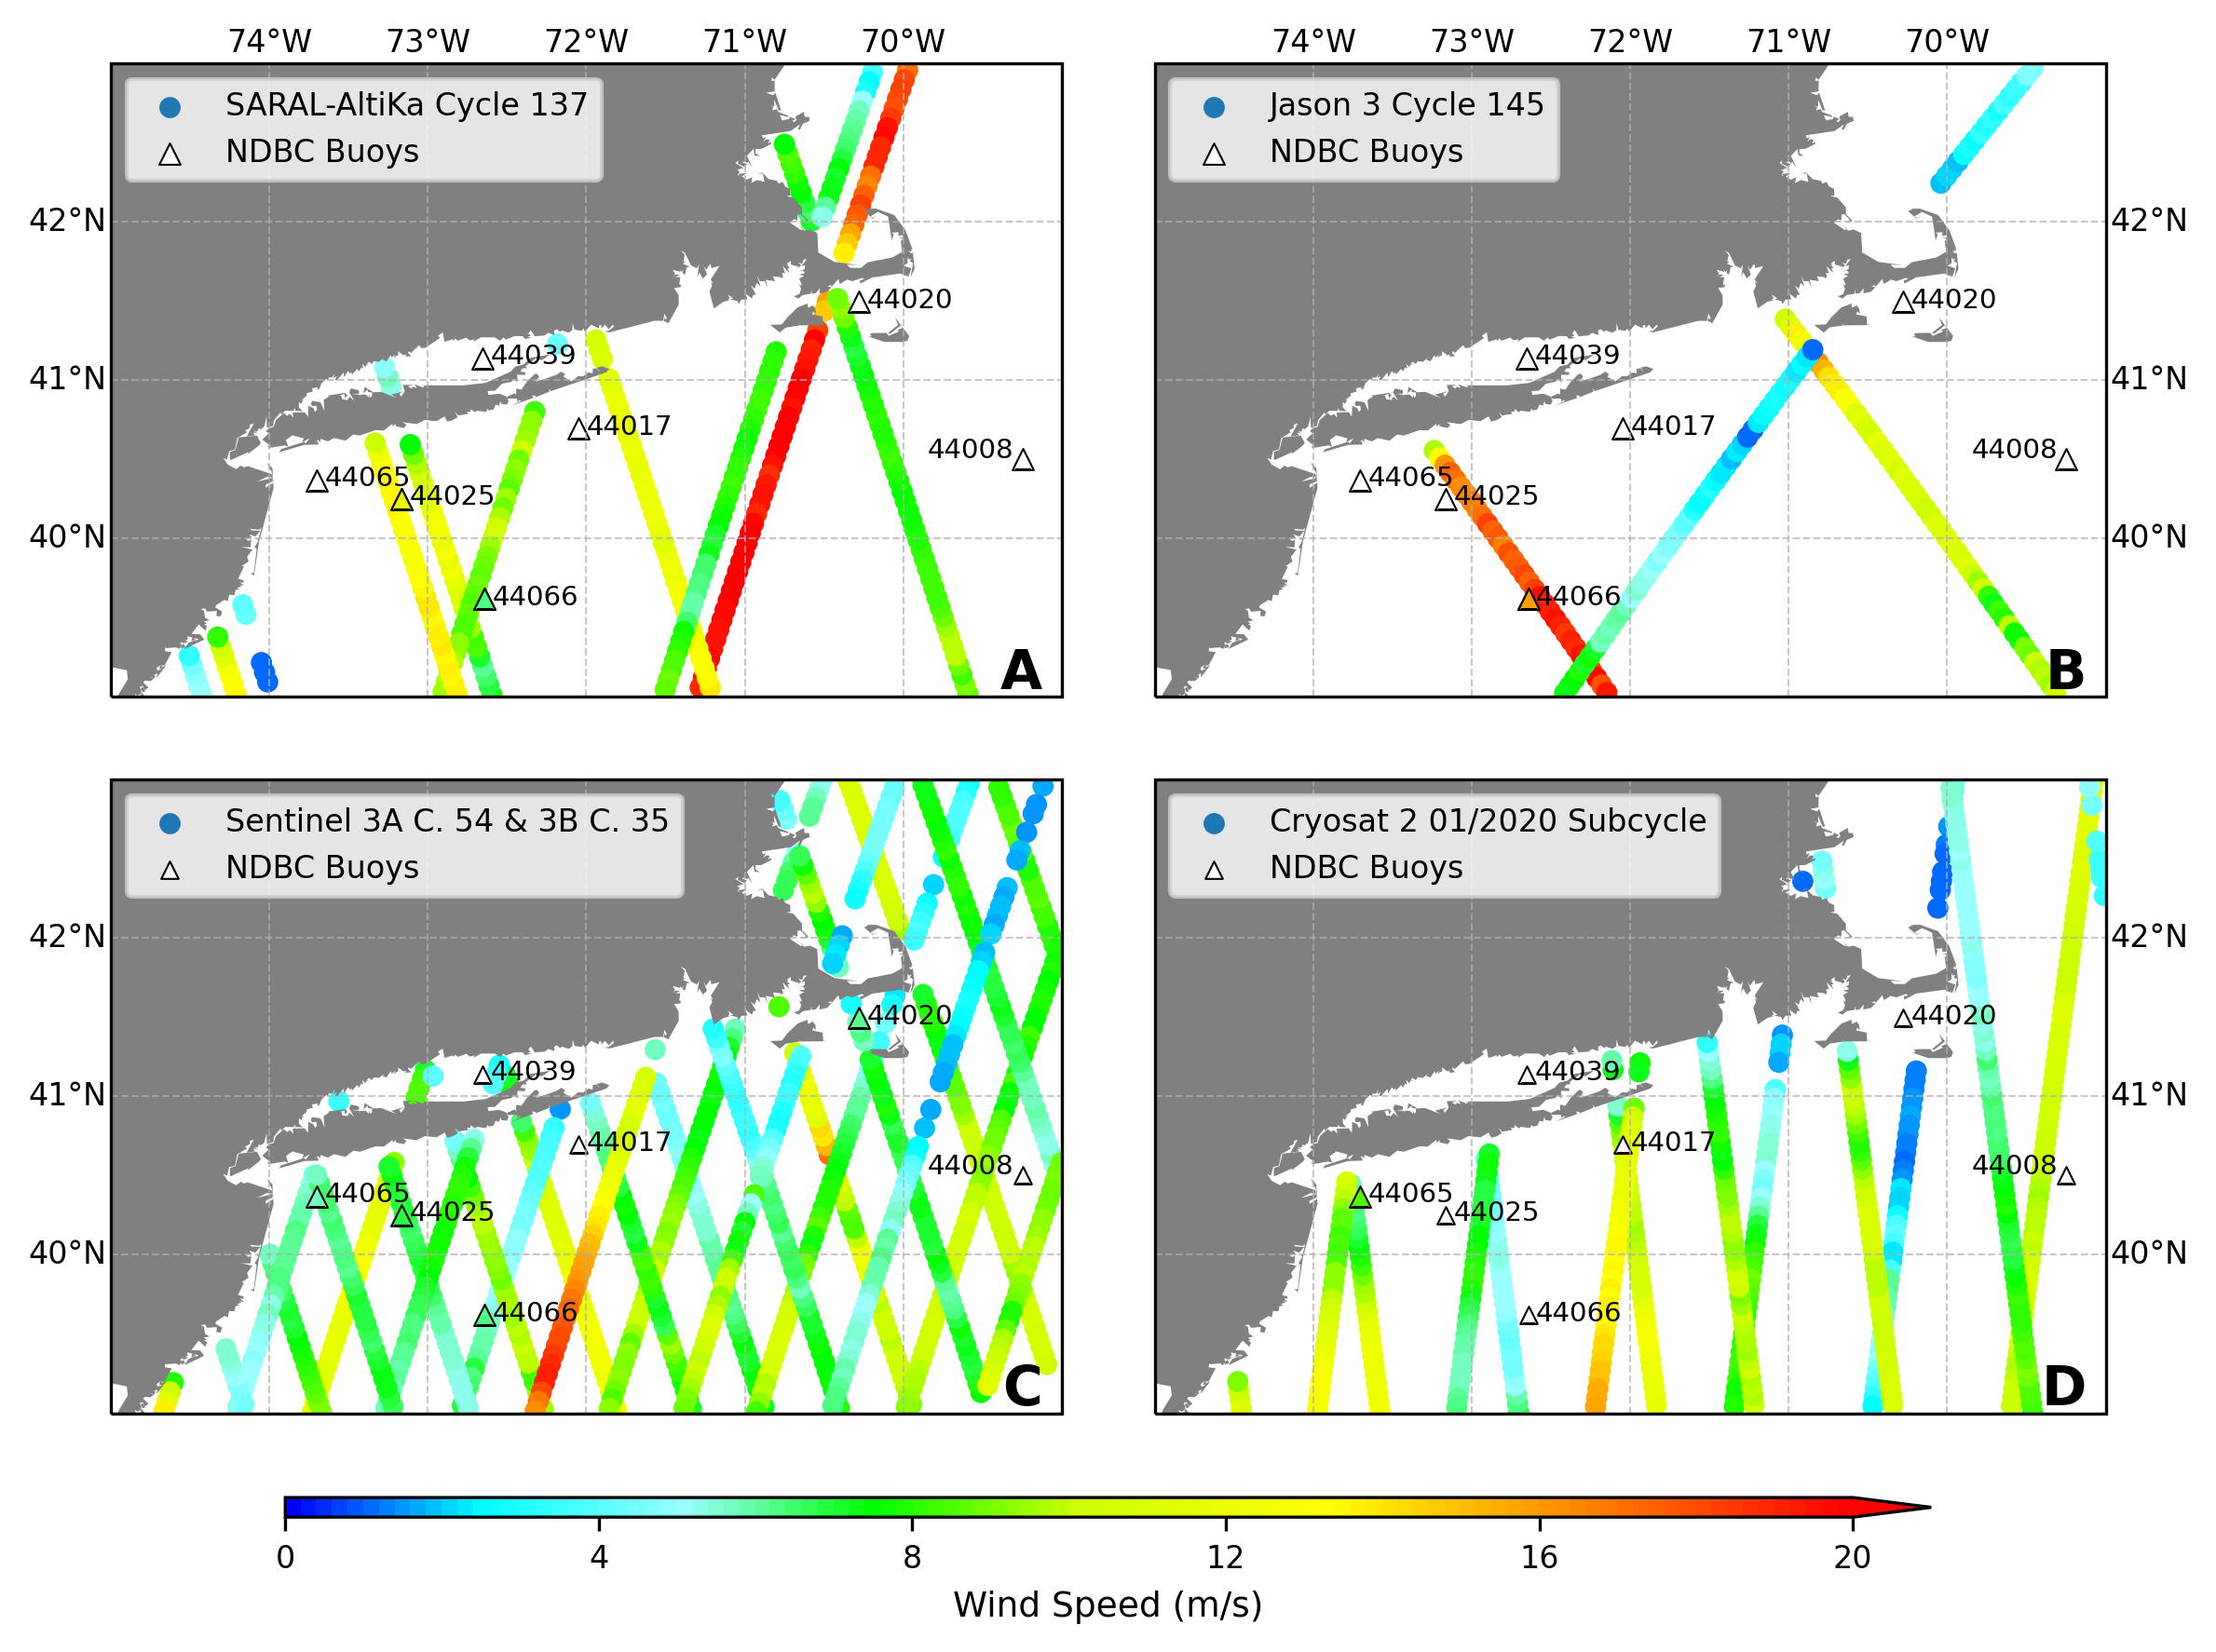
\includegraphics[width=0.95\linewidth]{Figures/Chapter5/SNE_obs_altimeter_col2.png}
%\decoRule
\caption{Altimeter tracks during January 2020 over SNE, including the buoys' locations and the collocated WS observations.}
\label{fig:altimeter_buoy_obs}
\end{figure}


Figure~\ref{fig:altimeter_buoy_obs} shows the altimeters tracks and WS observations over SNE during a specific cycle or subcycle in January 2020. Sentinel 3 A and B tracks are included in the same Figure~\ref{fig:altimeter_buoy_obs}C, and their combined dataset was used in the calculations because they are considered as the same mission with identical sensors. In the same Figure, the buoys' locations are depicted with triangles. The collocated observations are represented by colored triangles, whereas the buoys that do not match with the altimeters during their specific cycle or subcycle are left empty. This process described in \ref{collocation} was performed iteratively for multiple years, depending on the altimeters' data availability. The final collocated dataset contains both buoy and altimeter observations that were matched in space and time. Its sample size is expected to be relatively small, considering the range of the altimeter cycles (10 to 35 days) and the small sampling radius required in a coastal region.




\begin{figure}[H]
\centering
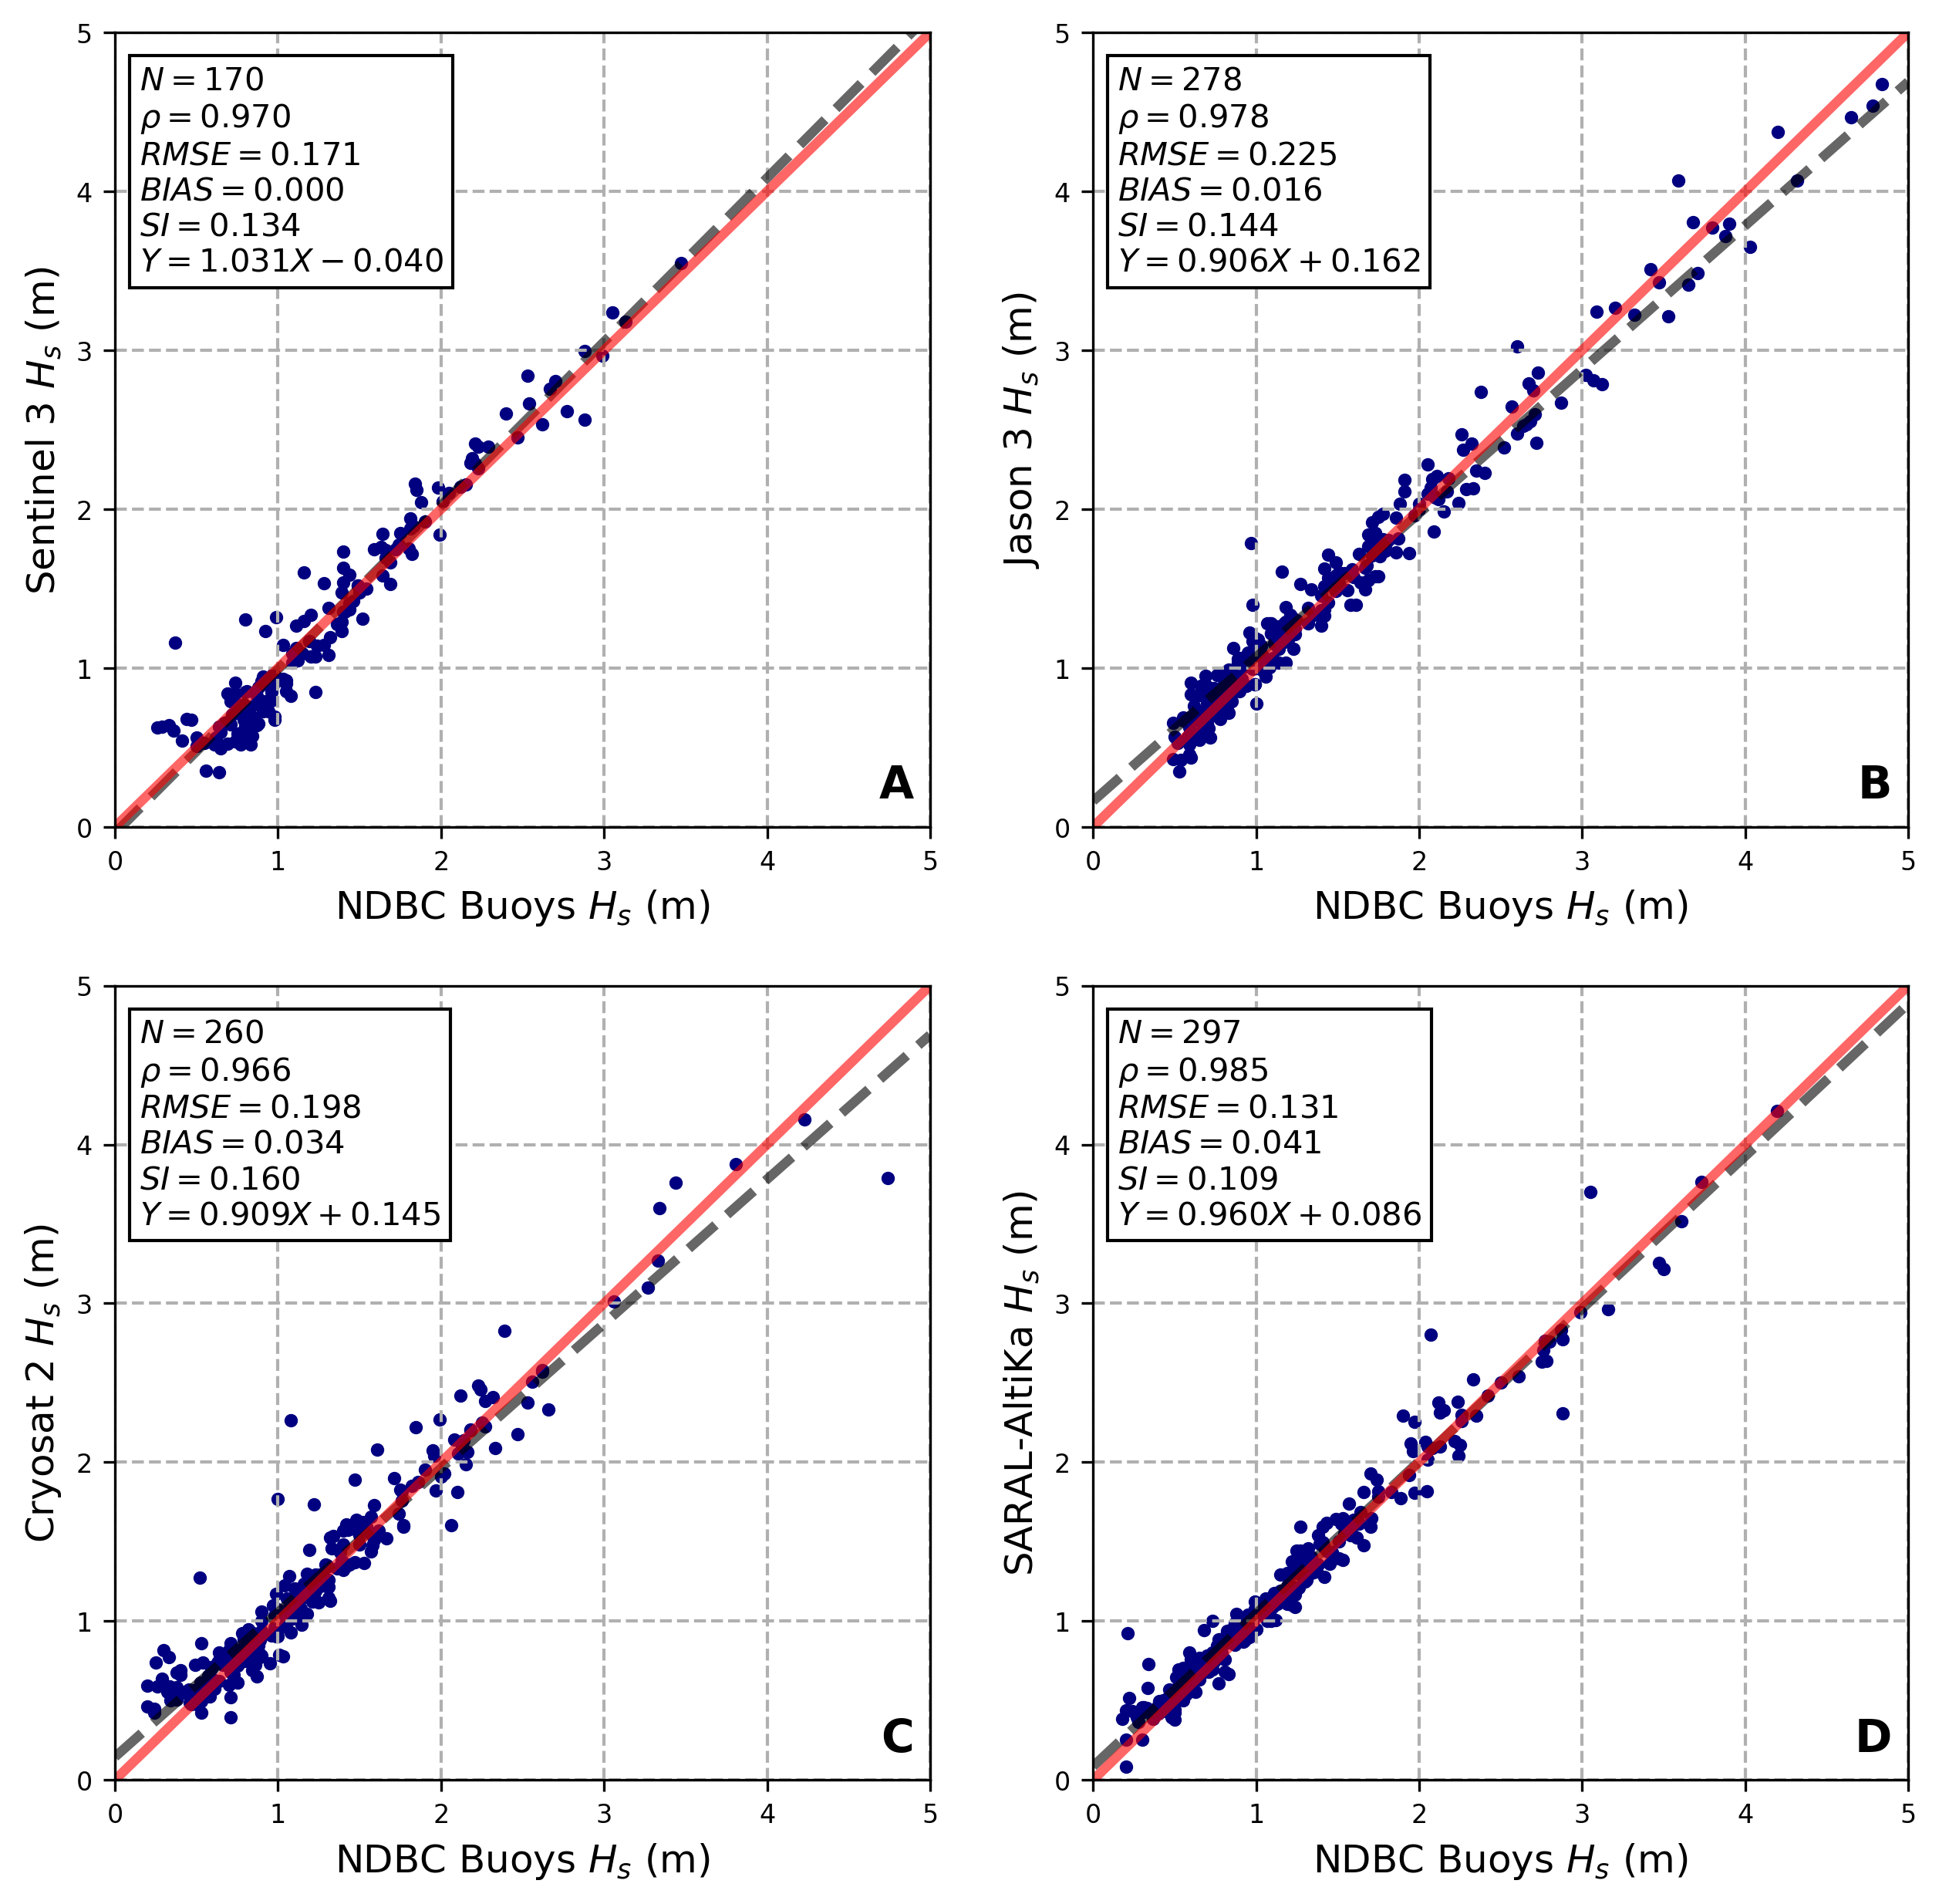
\includegraphics[width=0.79\linewidth]{Figures/Chapter5/validation_altimeters_wave1.png}
%\decoRule
\caption{Comparison of SWH between altimeter and in-situ observations.}
\label{fig:validation_wave}
\end{figure}


\begin{figure}[H]
\centering
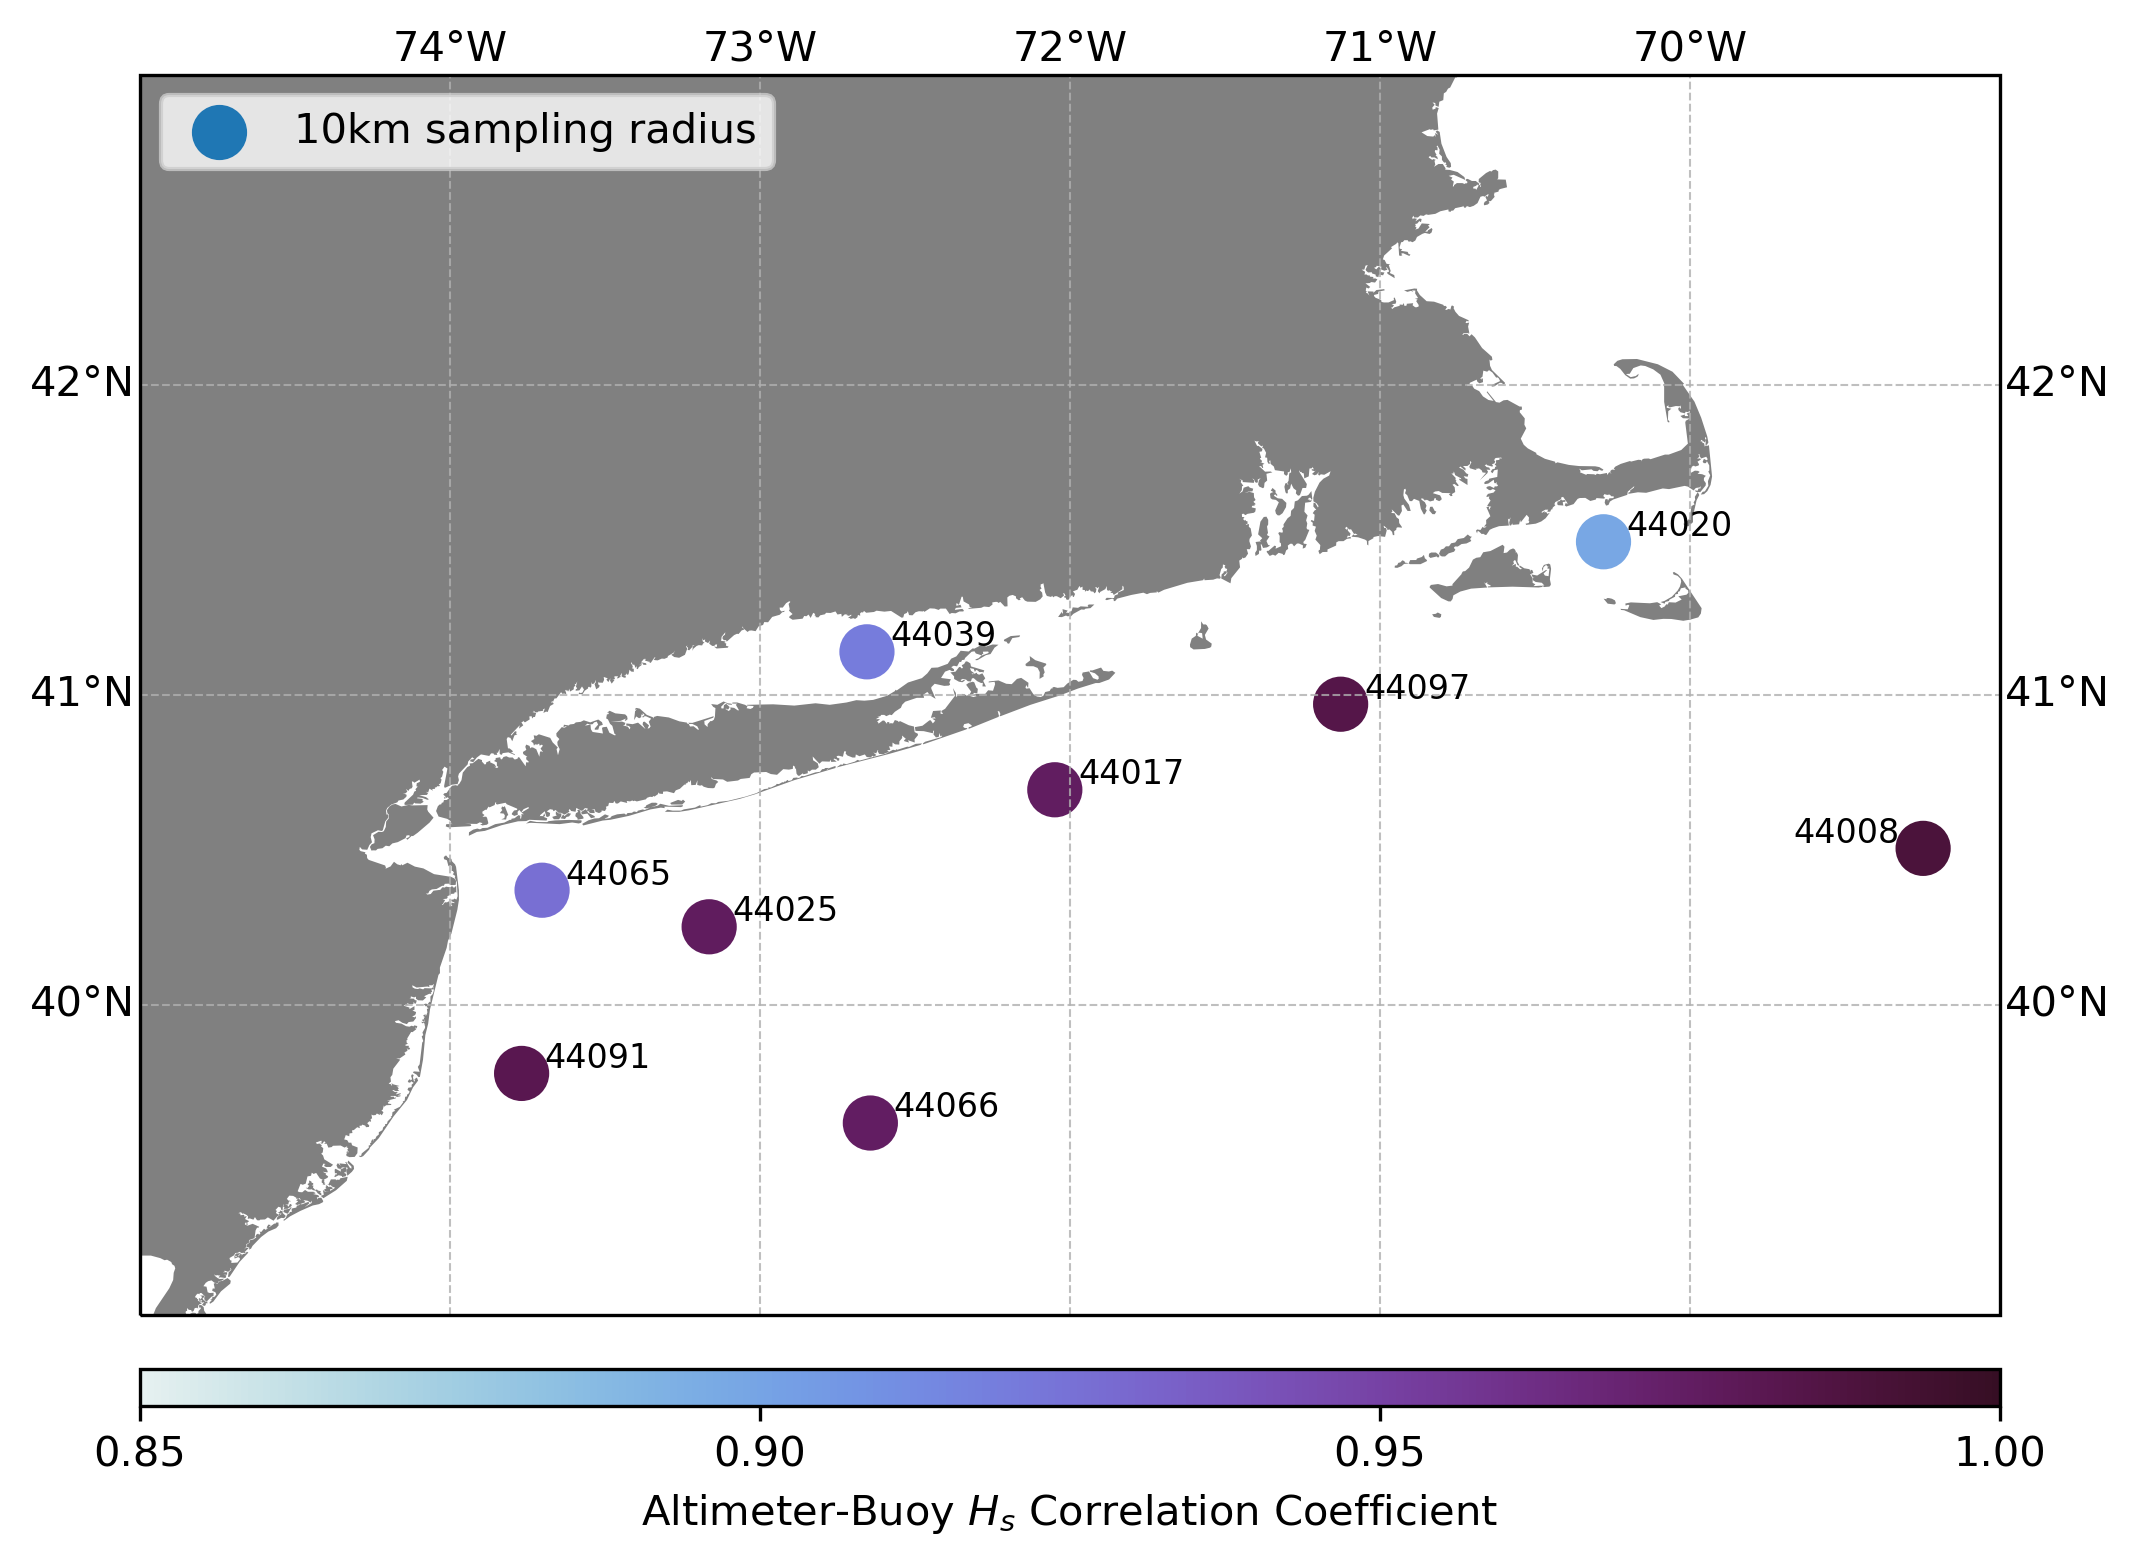
\includegraphics[width=0.79\linewidth]{Figures/Chapter5/buoy_altimeter_cor_coef_wave.png}
%\decoRule
\caption{Correlation coefficient map between altimeter and buoy SWH collocated data.}
\label{fig:corrcoef_wave}
\end{figure}



\begin{figure}[H]
\centering
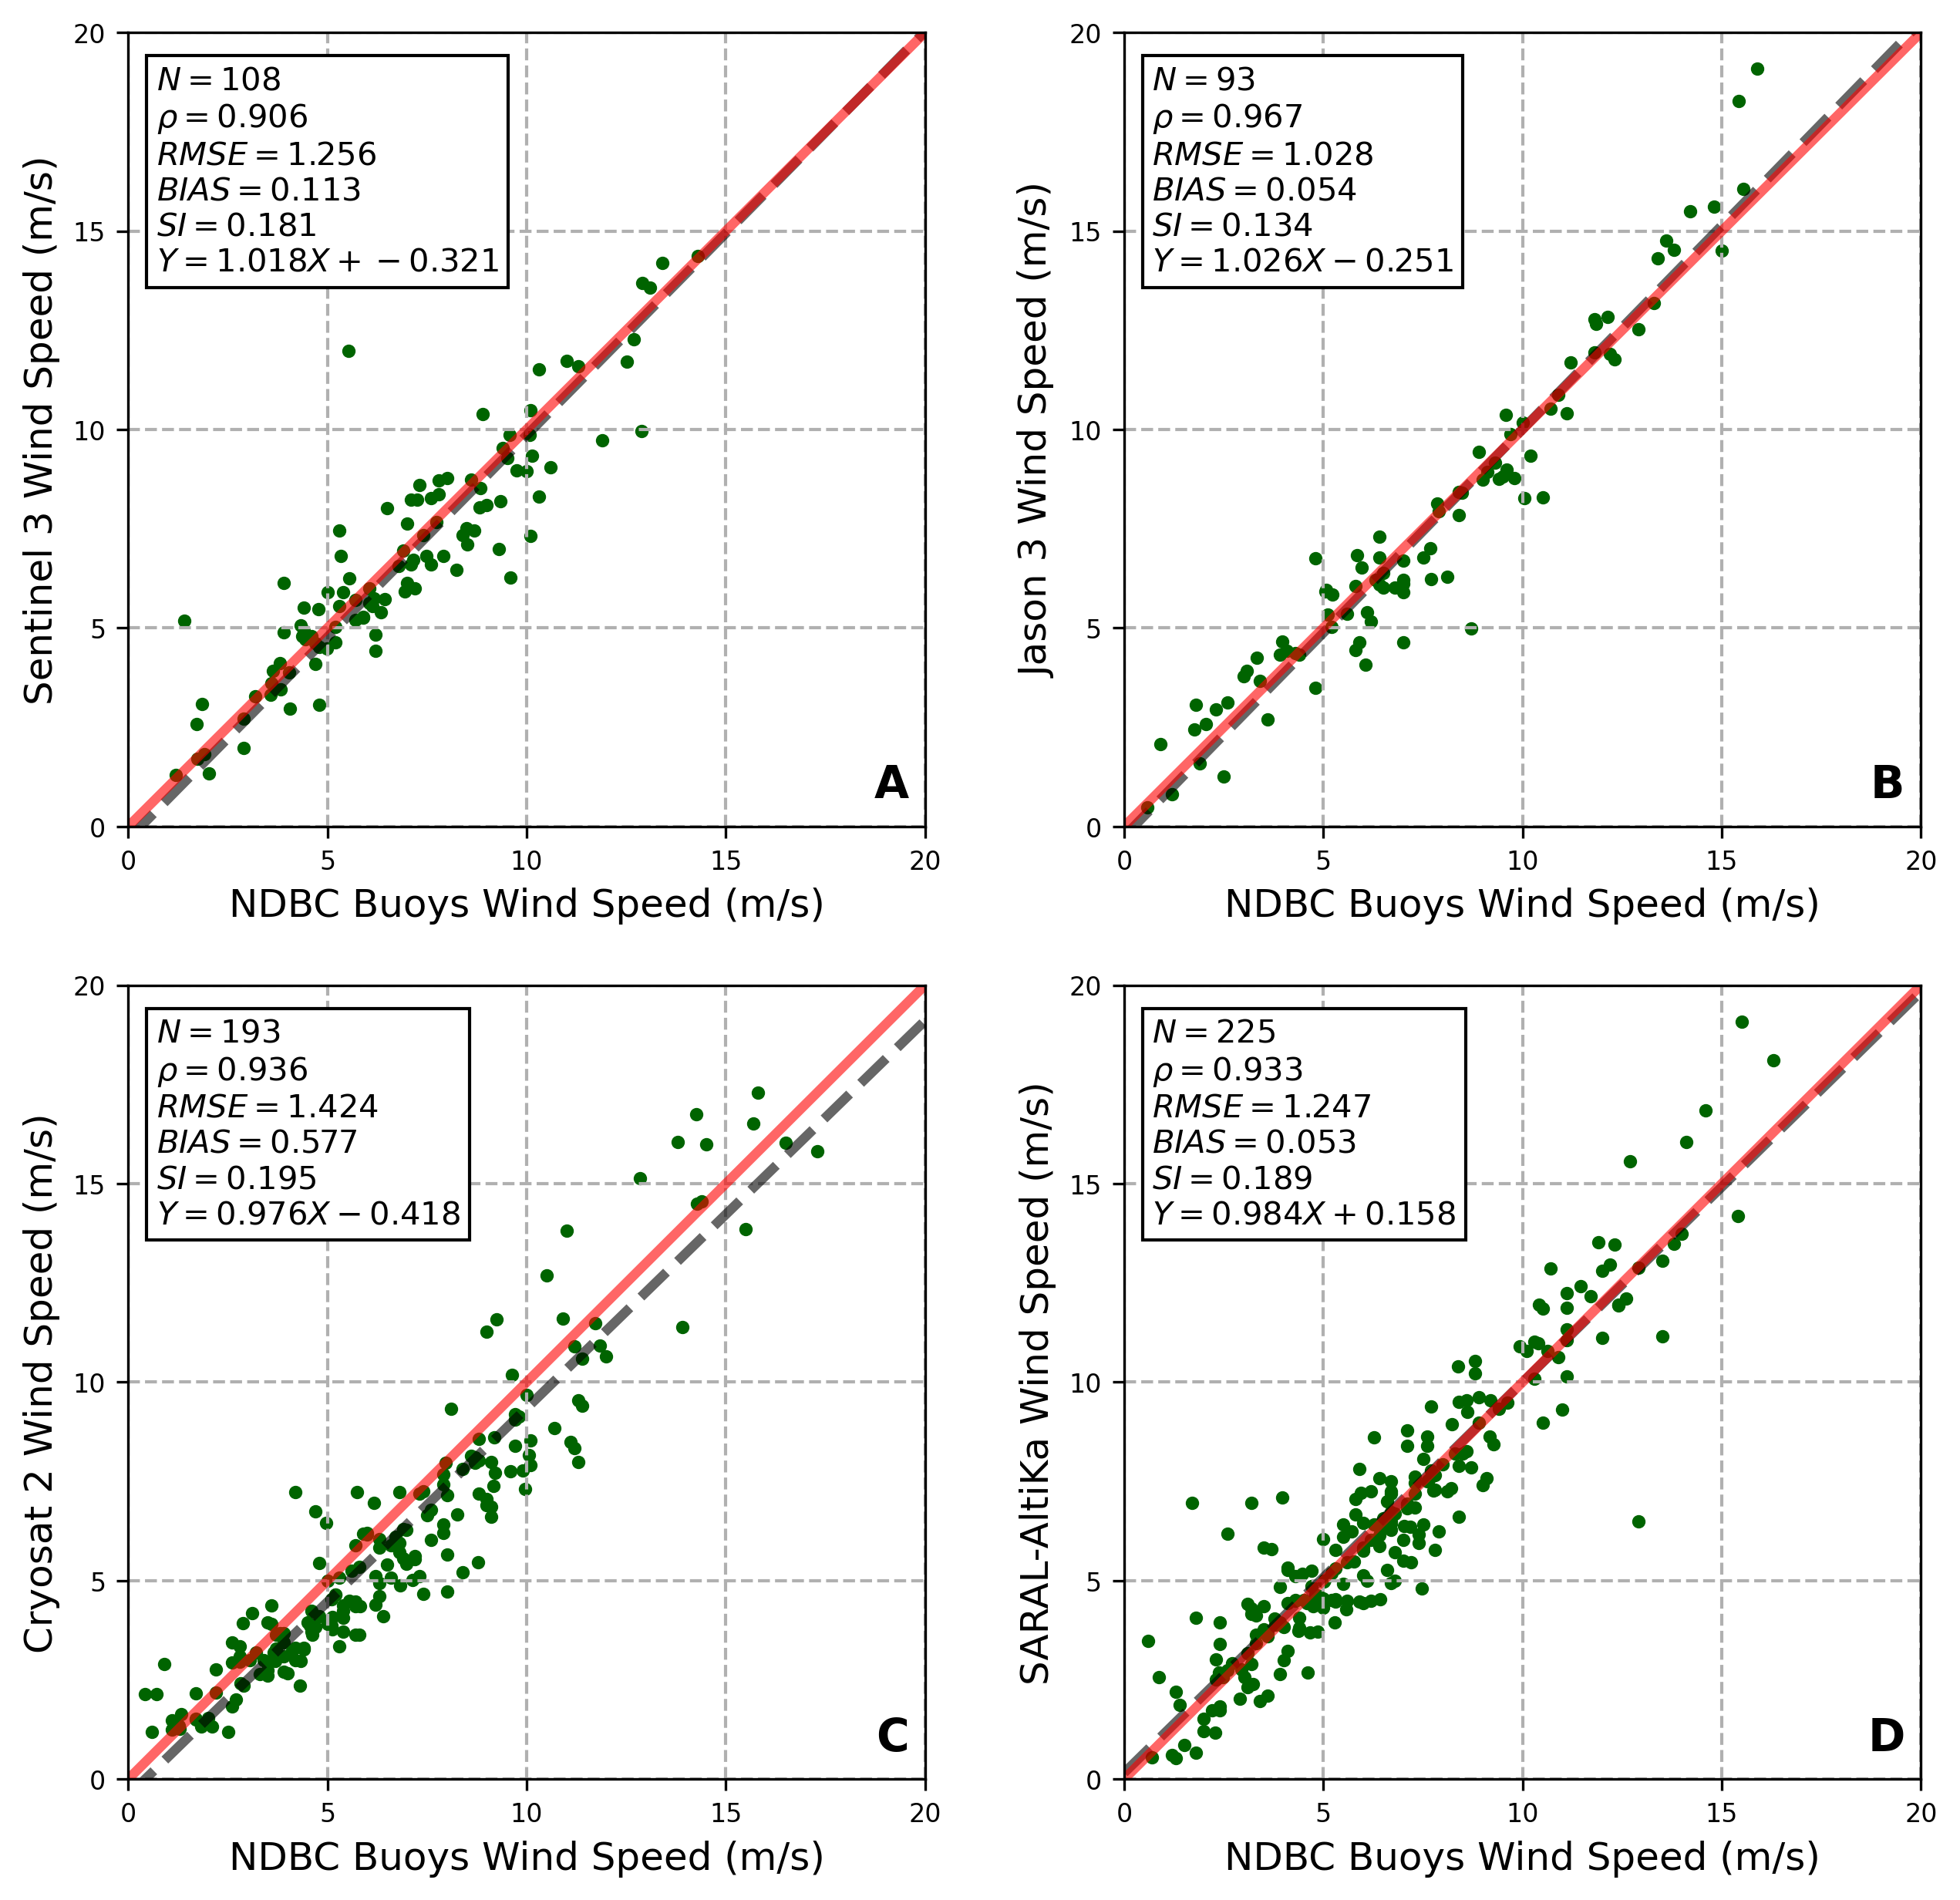
\includegraphics[width=0.79\linewidth]{Figures/Chapter5/validation_altimeters_wind3.png}
%\decoRule
\caption{Comparison of WS between altimeter and in-situ observations.}
\label{fig:validation_wind}
\end{figure}


\begin{figure}[H]
\centering
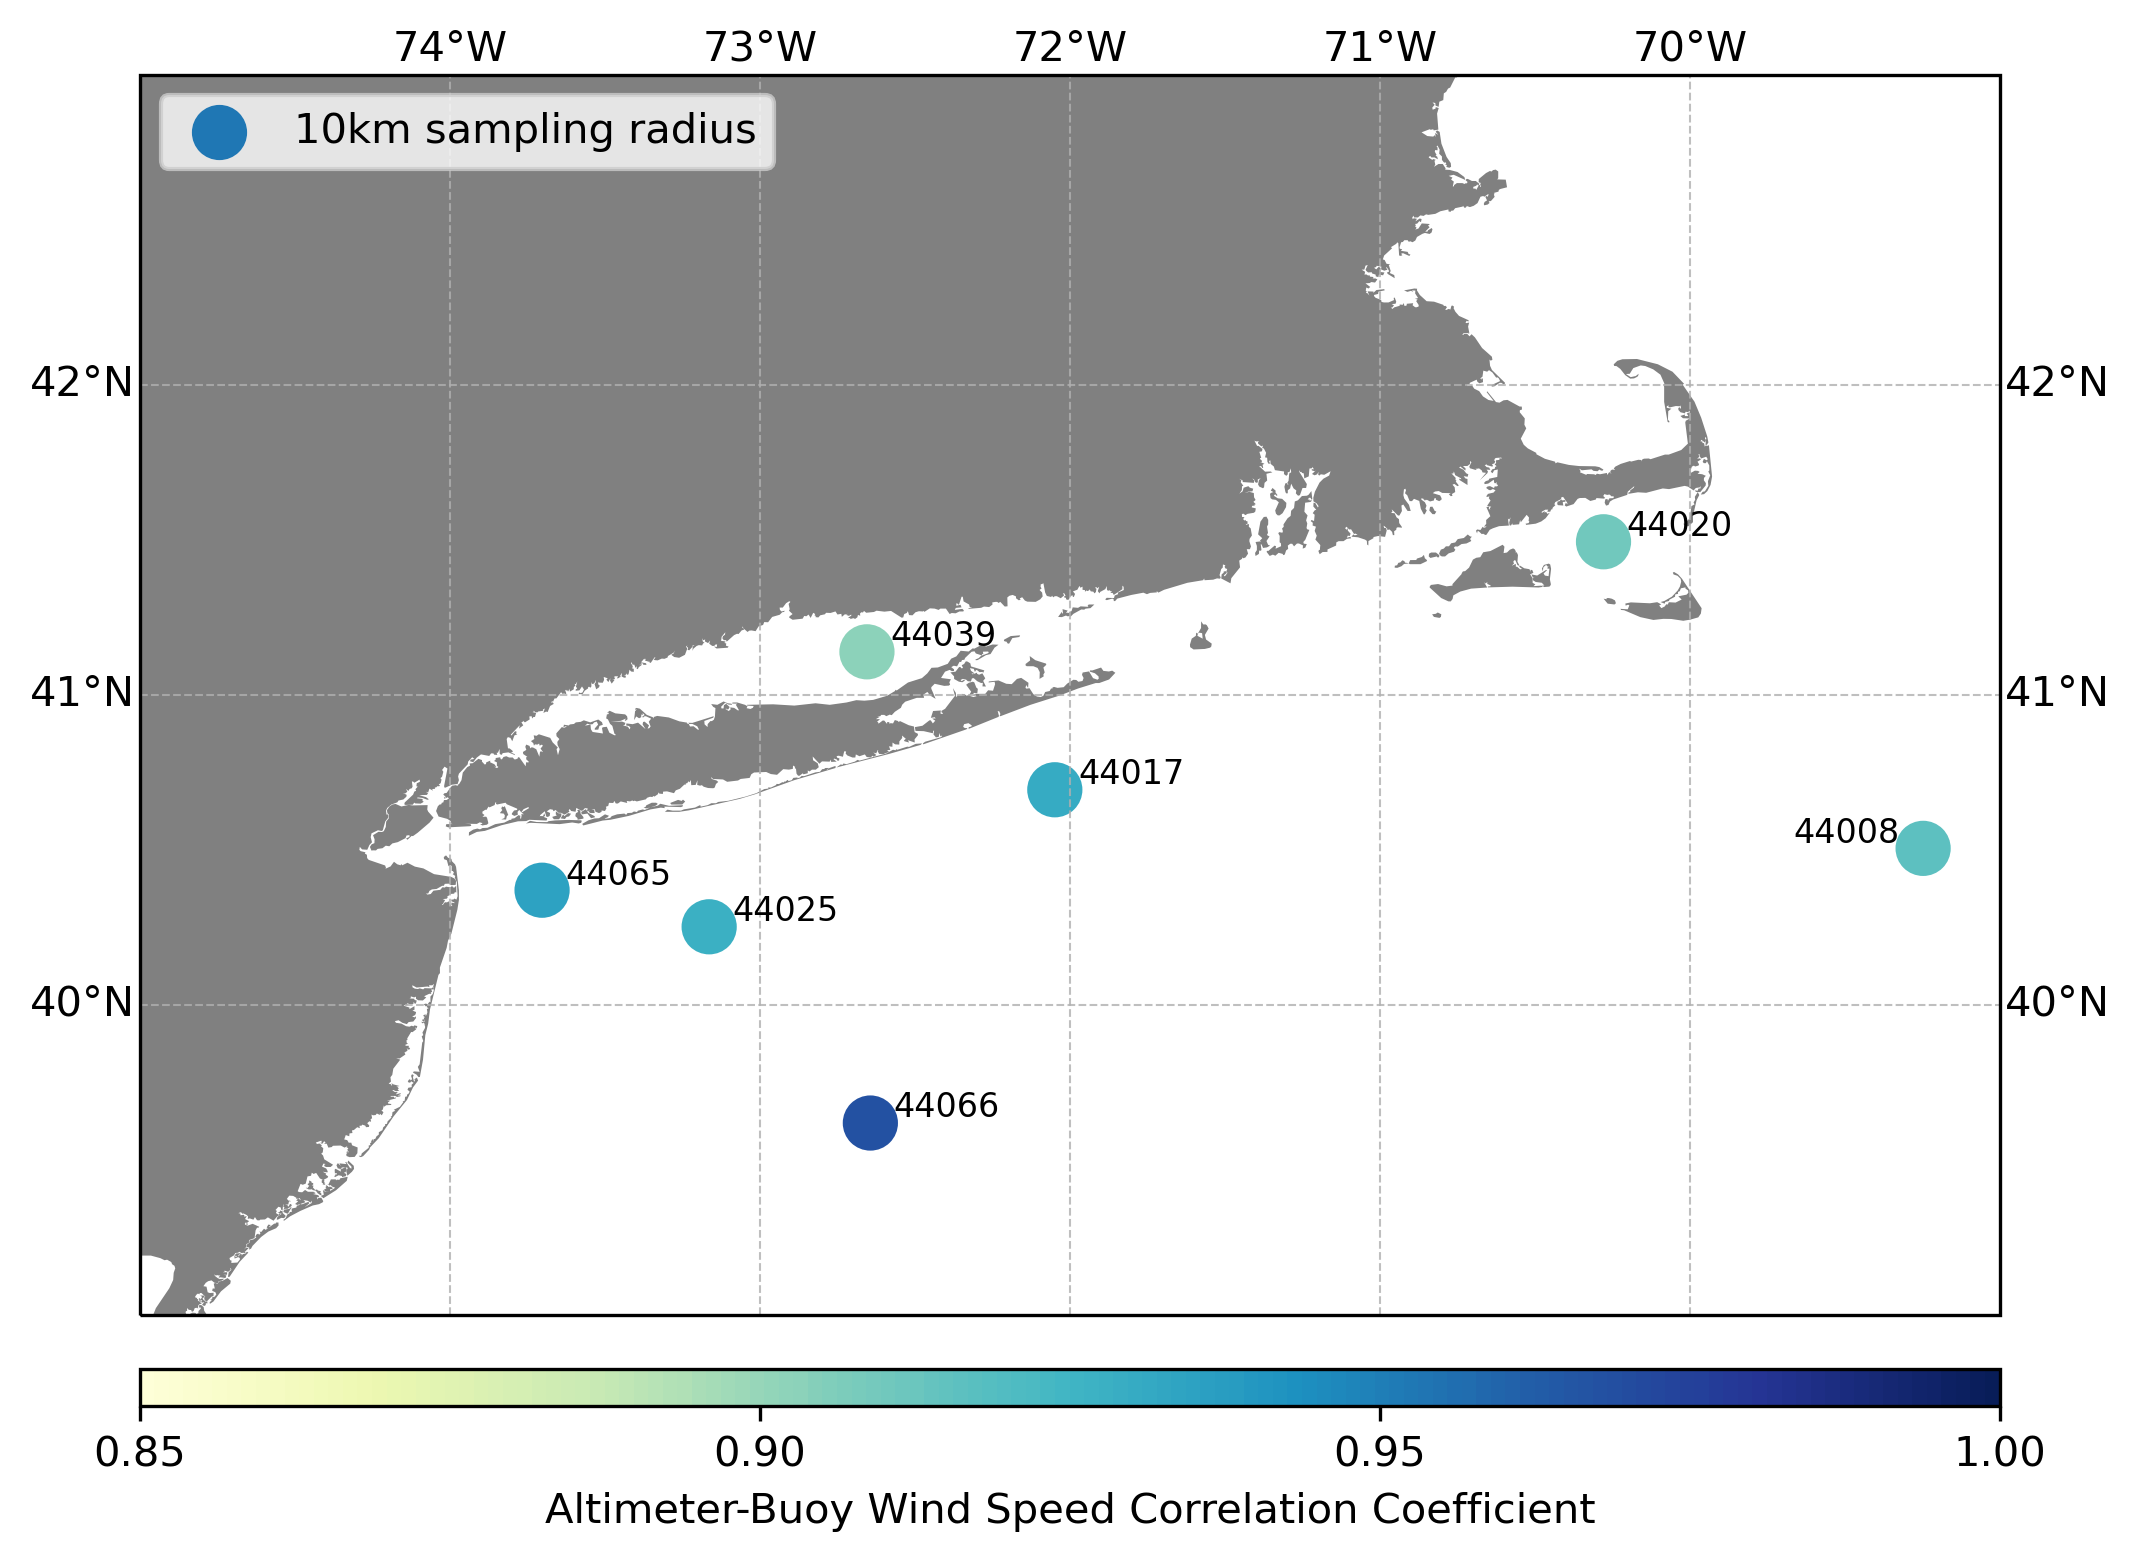
\includegraphics[width=0.79\linewidth]{Figures/Chapter5/buoy_altimeter_cor_coef_wind.png}
%\decoRule
\caption{Correlation coefficient map between altimeter and buoy WS collocated data.}
\label{fig:corrcoef_wind}
\end{figure}


The collocated dataset's WS and SWH comparison and also the evaluation statistics are shown in Figures~\ref{fig:validation_wave}, \ref{fig:validation_wind}. It is evident that due to the different number of buoys with available WS and SWH, the corresponding comparisons result from larger sample sizes for the SWH. The evaluation metrics and the slope of the regression line show that SARAL-AltiKa has the best overall agreement with the buoys. Although there are a few outliers, they do not significantly influence the close approximation to the buoys' ground truth values. The uncertainty is very low even for SWH values lower than 1 meter, which has been documented as a challenge due to the difficulty in estimating the leading edge slope in low sea states and a general limitation of the satellite altimetry \cite{Ardhuin2019}. A root mean squared error (RMSE) of 13 centimeters, a scatter index (SI) of almost 11\%, and a correlation coefficient of 0.985 emphasize these results. Sentinel 3 also matches the buoy measurements with a zero average bias, which could also be attributed to the small sample size. Despite the small bias and the high correlation, Jason 3 shows the largest RMSE. This result can be attributed to the considerable number of match-up observations representing SWH over 3 and up to 5 meters. Cryosat 2, which utilizes the oldest technology of the current altimeters, also shows a good agreement with the buoys regarding their correlation and the small bias. Still, it has the highest number of outliers reflected on the SI (16\%) and RMSE (19.8 cm). Figure~\ref{fig:corrcoef_wave} confirms the assumption that the agreement between the buoy and altimeter observations is worse at locations with proximity to the land due to the challenges of coastal altimetry described in \ref{AltimetryPrinciples}. Generally, the agreement is exceptional in terms of correlation statistics, as the SWH correlation coefficient is well over 0.9 in almost every location. The highest correlation coefficient was calculated for the open ocean buoy 44008 and the lowest for the sheltered buoy 44020, located in the Nantucket Sound.

The WS comparison is more challenging, primarily due to the smaller sample size of the collocated dataset. Except for the lower number of stations with available wind data (7), the WS times series also contain more gaps than the SWH. The agreement in terms of statistics is best for Jason 3, but all collocated observations are located in a specific region surrounding the open ocean buoy 44066. On the other hand, SARAL-AltiKa has the largest sample size and collocated measurements at almost every buoy location. The statistics show good agreement with the buoy data with a minimal overall bias (0.053m/s). The comparison of Sentinel 3 with the buoys is sensitive to outliers due to the small collocated sample size, and it has the lowest correlation coefficient among all altimeters. Still, the RMSE (1.256m/s) and the bias (0.113m/s) are small and comparable to the values in the performance reports disseminated after every completed cycle. The worst performance belongs to Cryosat 2 with substantial bias (higher than 0.5m/s). However, the statistics are comparable with the target accuracy of 0.5m/s bias and 2m/s RMSE of the WS estimation from scatterometers \cite{Saldana2002}. Figure~\ref{fig:validation_wind}C shows an apparent underestimation of low WS (0-10m/s) and an overestimation of the higher WS values (10-20m/s), although the sample size is not as large for the higher WS. Figure~\ref{fig:corrcoef_wind} shows that for the WS, the location with the best agreement with altimeter data in terms of the correlation coefficient is the open ocean buoy 44066 (higher than 0.95), and the worst is the sheltered buoy 44039 (almost 0.9) located in the Long Island Sound.

Considering the expected differences \cite{Monaldo1988} and results from similar studies \cite{Sepulveda2015, Yang2019}, altimeter SWH is consistent with the buoy observations. The comparison also showcases the strength of SARAL-AltiKa in coastal regions due to its higher resolution and lower noise in the observations \cite{Ardhuin2019, Bonnefond2018}. Validation of altimeter WS with the available buoys in SNE is more challenging due to the relatively small sample size and the sampling radius. However, the overall statistics show good agreement between the two data sources. Although studies related to the altimeter WS algorithms \cite{Abdalla2007, Gourrion2002, Lillibridge2014} define the ocean surface WS as the WS at 10 meters height, the buoy measurements were not adjusted. The adjustment, assuming neutral boundary layer stability, induced systematic biases, and worse overall performance regarding the statistics.




%------------------------------------------------------------------------
-------------------


\section{Wind and Wave maps based on satellite altimeter data}\label{}

In the previous section, we evaluated each altimeter's performance with respect to in situ observations and their collective dataset with increasing distance to the coast. This section attempts to utilize altimeter data and the methodology described in \ref{variogram_kriging} to create maps of the surface WS and the SWH in the SNE region for the winter and summer seasons. One goal is to estimate the WS and SWH in unobserved locations by interpolating the altimeter observations to a regular grid. The selected $0.125^{\circ}\times0.125^{\circ}$ grid is consistent with the distance between altimeter observations on each track (6-7 kilometers) and the altimeter's effective footprint (2-7 kilometers).  We selected data from 2019 primarily because it is the first year with data available from all five altimeters, Jason 3, Sentinel 3 A and B, SARAL-AltiKa, and Cryosat 2. Therefore, we filled spatial gaps by adding as many neighboring observations as possible. One disadvantage of the buoys' fixed point locations is that we cannot make assumptions of the geophysical parameters' transition between each station or how the observations are correlated from point location to another. It is neither feasible to have a dense network of in situ stations. Besides, only CDIP buoy 44097 is located inside the offshore wind projected areas. Thus, one of the benefits of this section's results is deducing the WS and SWH gradient from the interpolated maps and its uncertainty.

Figure~\ref{fig:kriging_wind2019} is the map of the interpolated WS altimeter observations for the winter (A) and the summer (B) seasons. Grey contour lines have been added to distinguish areas with a 0.5m/s difference, primarily due to the significant WS gradient during winter. Generally, WS increases with increasing distance to the coast due to the sea surface's lower roughness length and the land's decreasing influence on the transition from a coastal area to the open ocean. Besides, we showed in \ref{diurnal_variability} and \ref{seasonal_variability} that SNE is characterized by substantial seasonal variability, especially in the open ocean where the difference of the average WS between the summer and winter seasons is over 4m/s. The WS maps show general agreement with this result as most areas present significant seasonal differences. This feature is critical for offshore wind energy because the wind turbines start operating at a cut-in WS of 3-4 m/s, and their rated WS of maximum capacity is between 11 and 16 m/s. However, the altimeter WS maps represent interpolated surface WS values, and the WS values are expected to be higher at the turbine height. The WS maps indicate values between 4 to 6 m/s for the summer and 6 to 10 m/s for the winter season, respectively. During summer 2019, coastal areas and the northeastern part of the region showed the lowest WS values, and the area between $39^{\circ}-39.5^{\circ}$N and $72.5^{\circ}-71.5^{\circ}$W the highest. The region of peak WS during winter is at $40^{\circ}N$ and $70.5^{\circ}$W. There are also two high WS regions, one south of the eastern Long Island and the other north of Cape Cod, MA. The lowest WS can be identified close to the New Jersey shores and the Massachusetts Bay and Boston area. The notable WS gradient could be attributed to the local phenomena present during winter and described in \ref{study_area}. The case study of an extreme event in \ref{extreme_event} also showed that the WS is at its highest during the passing of storms. Therefore, when altimeters capture several extreme events, our estimations are sensitive to extreme WS values. The opposite applies if altimeters miss the passing of the storms. On the contrary, slow-moving, high-pressure systems are mostly present during summer over SNE, decreasing the variability between consecutive altimeter tracks. On average, there are two altimeter tracks available every day over SNE. Still, these tracks represent the satellites' passing over specific regions each time, and they do not cover the whole domain. Therefore, our estimations have spatial and temporal limitations.

Figure~\ref{fig:kriging_wave2019} contains the interpolated SWH maps for the 2019 winter (A) and summer (B) seasons. Figure~\ref{fig:buoy_wave_seasonality} showed that generally, there is strong SWH seasonal variability in the region, especially in the open ocean and as we move further offshore. However, the seasonal variability is almost insignificant in areas surrounded by land or islands like the Nantucket sound, mainly due to the relatively low WS seasonal variability and the small percentage of swell waves reaching the domain. Therefore, the higher gradients of SWH during the winter that are depicted in Figure~\ref{fig:kriging_wave2019}A with respect to Figure~\ref{fig:kriging_wave2019}B are expected. On average, SWH ranges from 1 meter close to the coast to over 2 meters in distances over 100 kilometers offshore during the winter. During summer, SWH is low in the coastal area north of Cape Cod Bay, and the highest values are estimated at approximately $70^{\circ}$W and $39^{\circ}$N, the same region of peak SWH during winter 2019. Based on the climatological averages available in Tables~\ref{tab:wave_distribution_winter} \ref{tab:wave_distribution_summer} and the interannual variability Figure~\ref{fig:b44020_wave_inter}, the interpolation maps overestimate the SWH very close to the coast and in areas where the influence of swell waves is minimized. This result depicts one of the disadvantages of the kriging methodology and interpolation in general.  Kriging provides the best linear unbiased prediction based on the modeled variogram. Still, the topography's constraints and, consequently, the coastal wave dynamics in a semi-enclosed area or inside a sound are not considered for the estimations. Therefore, they are biased with substantial deviations from the expected values.

\begin{figure}[H]
\centering
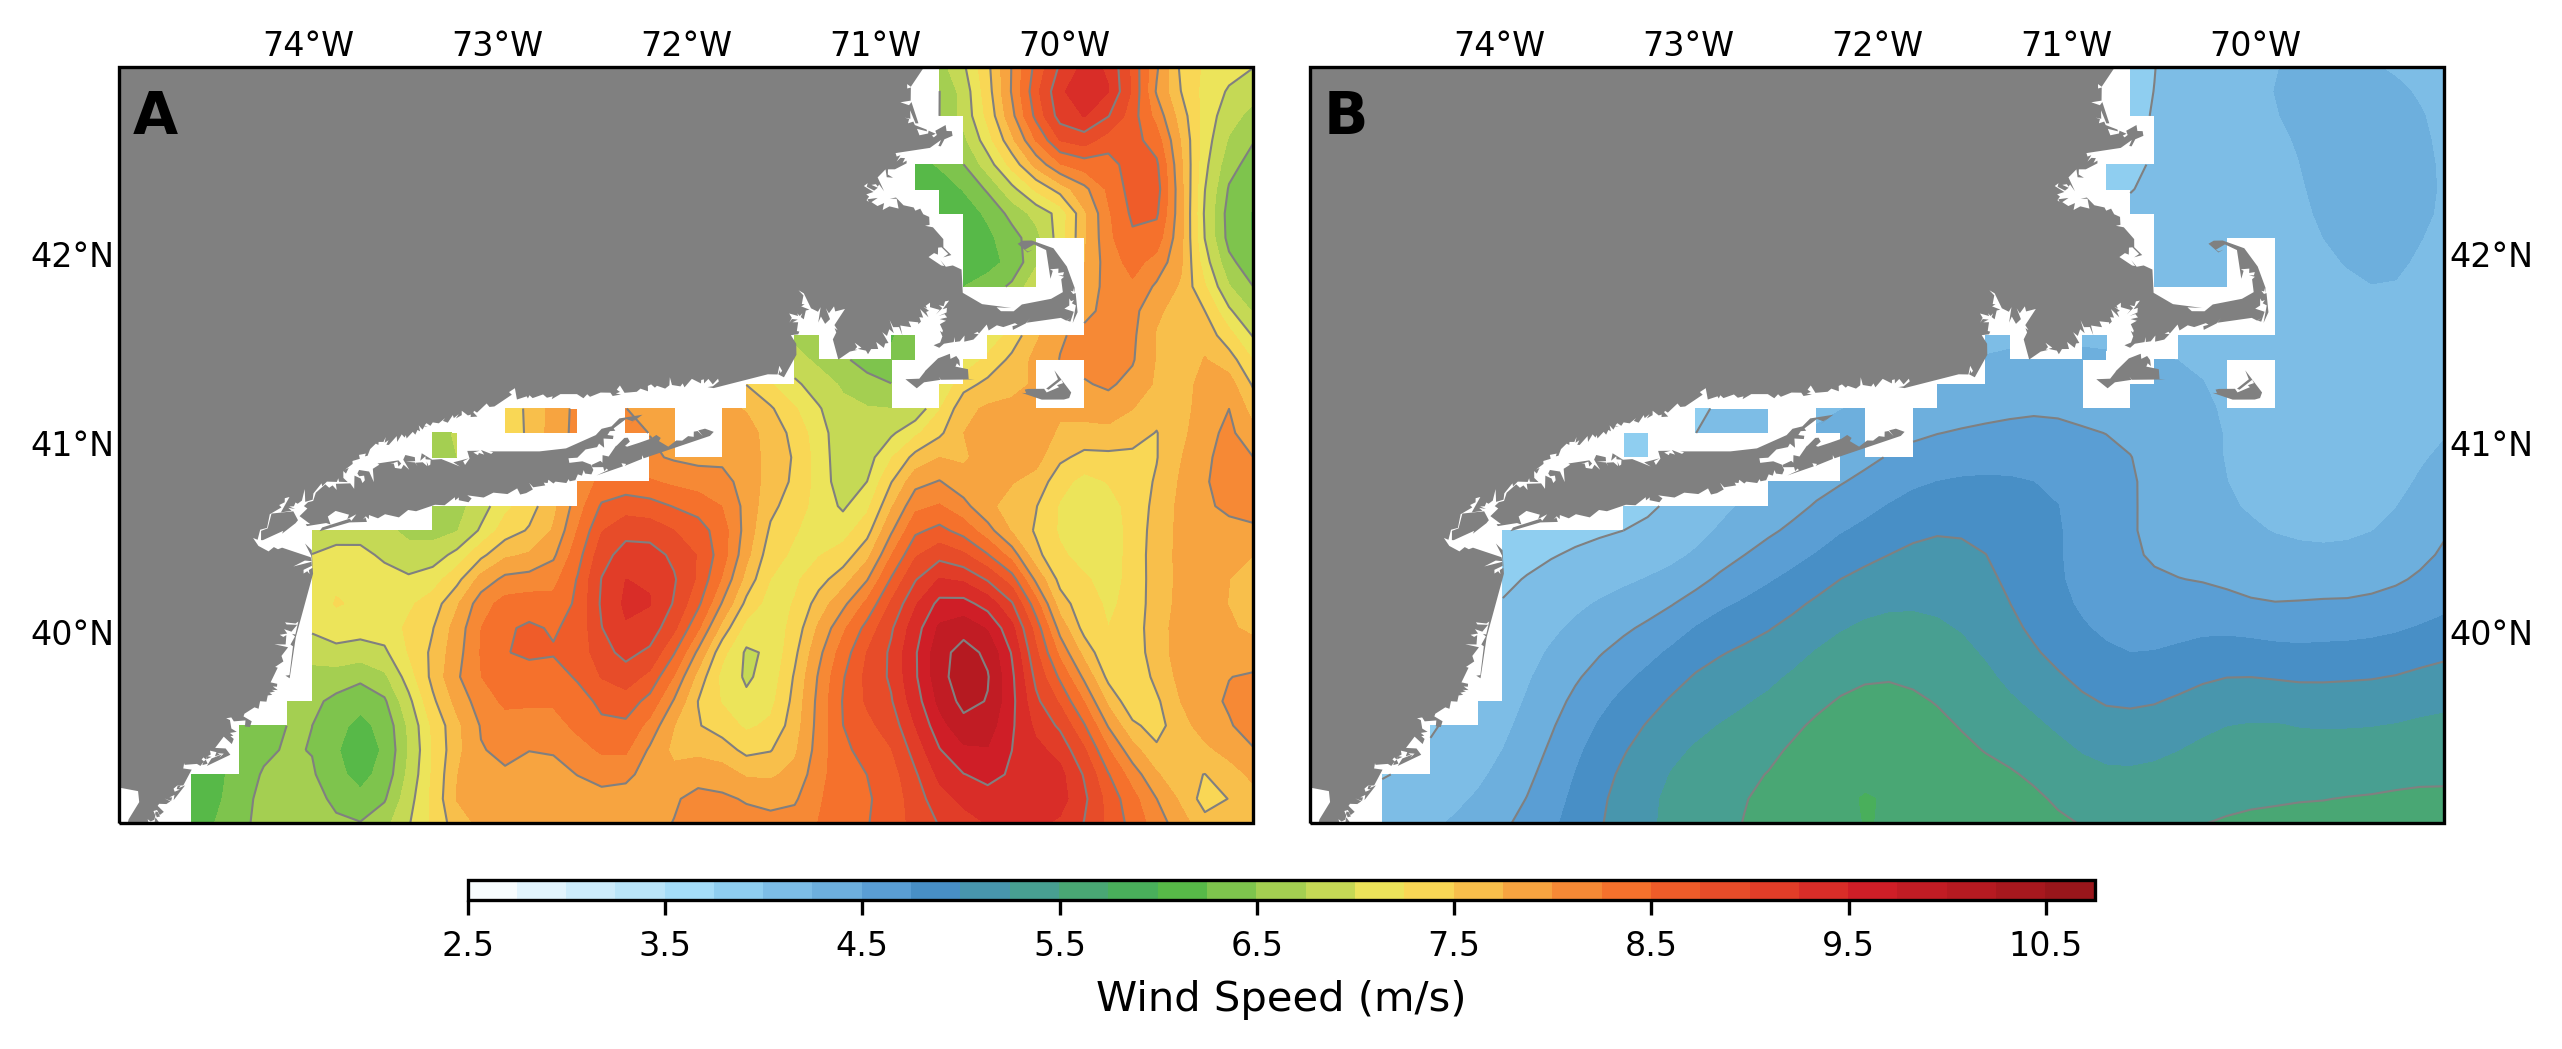
\includegraphics[width=0.95\linewidth]{Figures/Chapter5/kriging_wintsumm2019_wind.png}
%\decoRule
\caption{Surface WS kriging interpolation maps of altimeter data for the 2019 winter (A) and summer (B) seasons.}
\label{fig:kriging_wind2019}
\end{figure}


\begin{figure}[H]
\centering
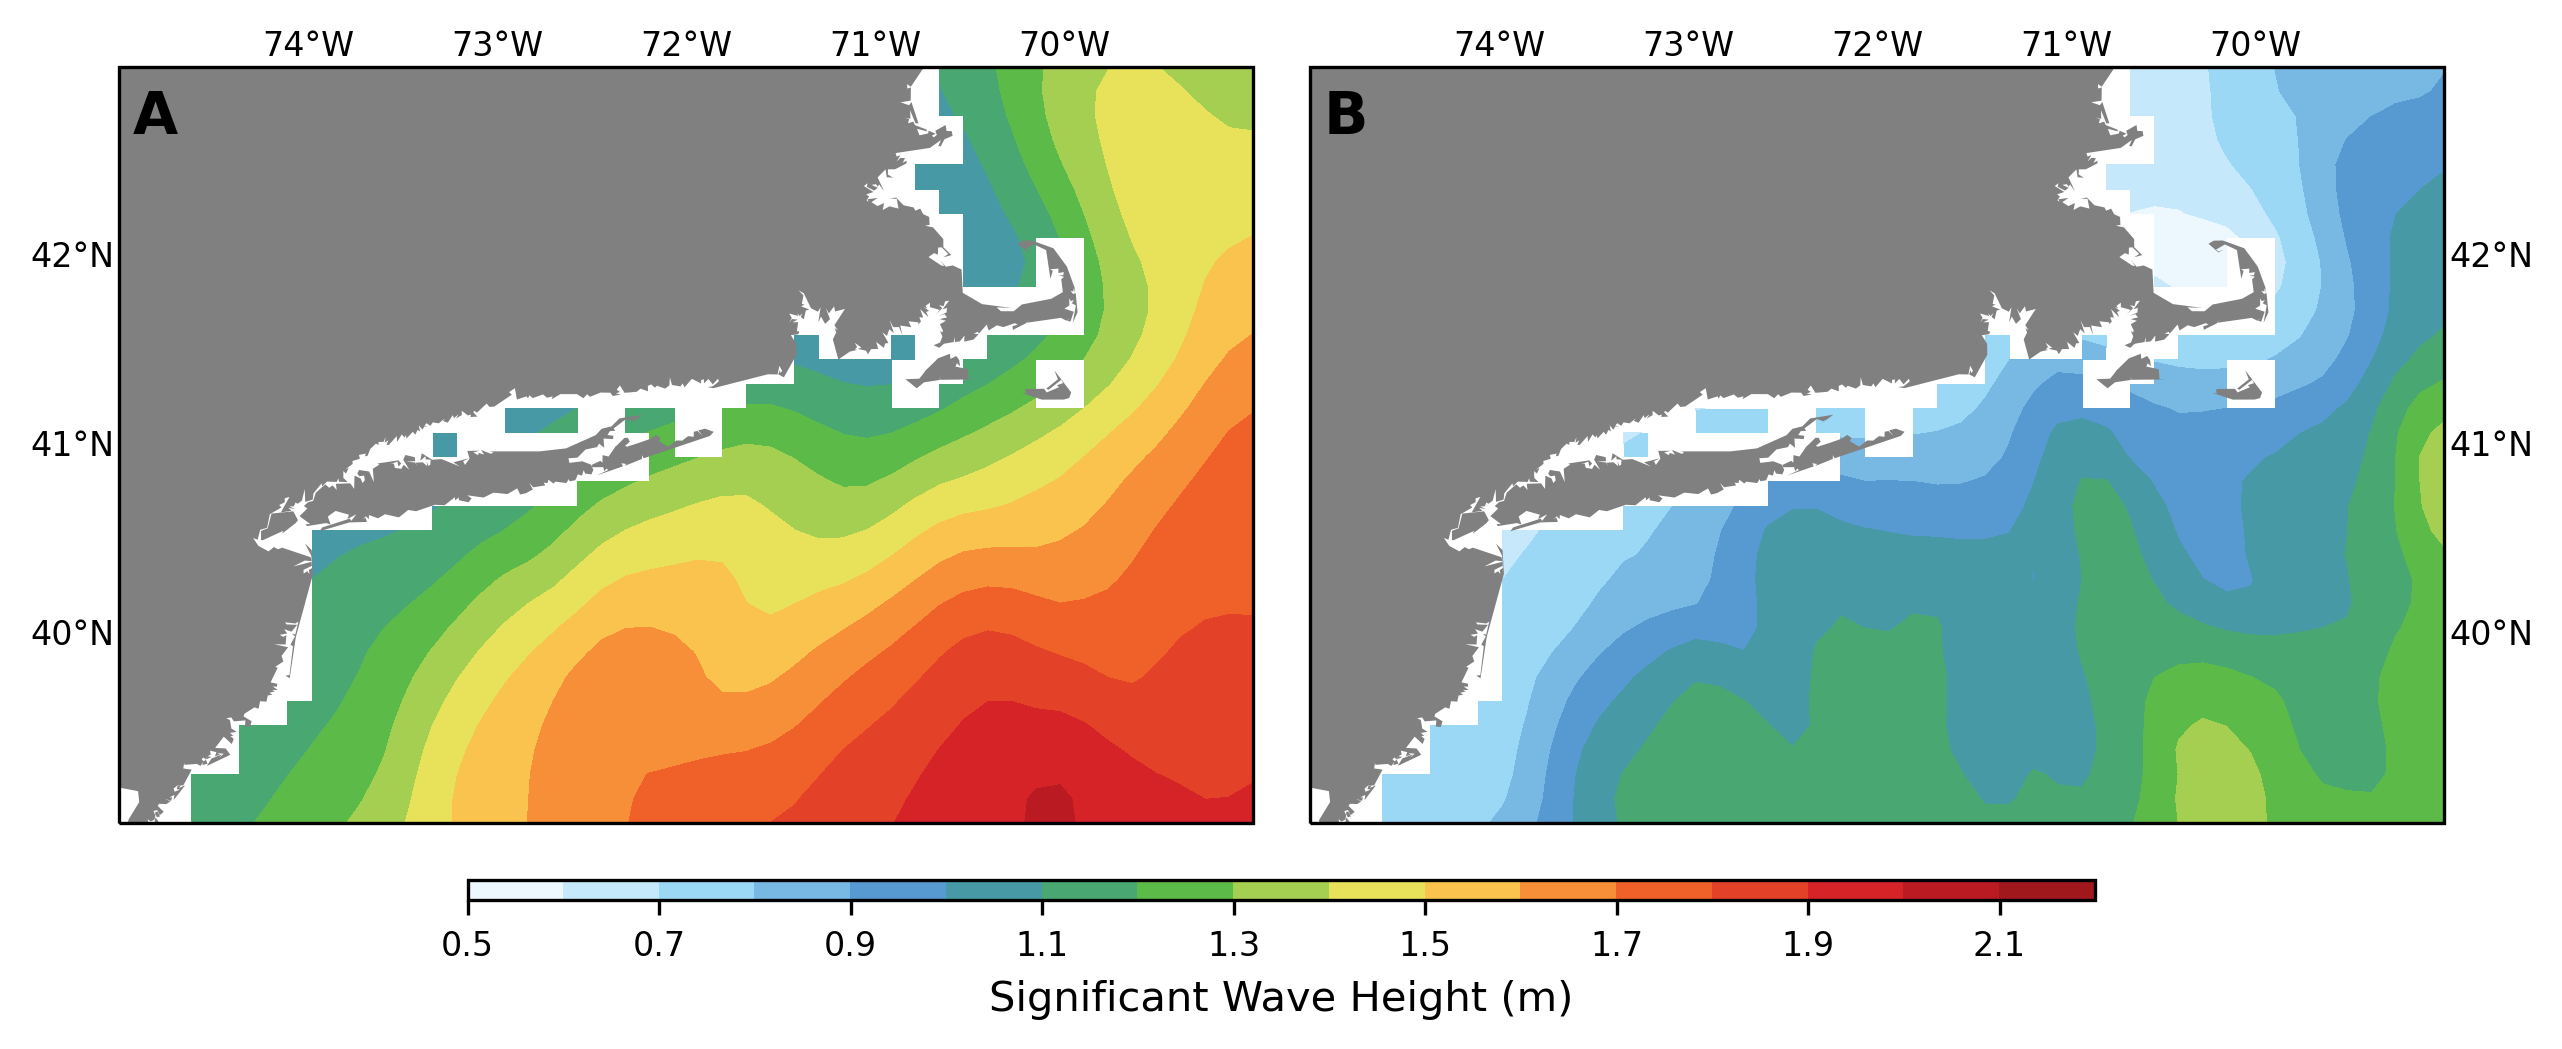
\includegraphics[width=0.95\linewidth]{Figures/Chapter5/kriging_wintsumm2019_wave.png}
%\decoRule
\caption{SWH kriging interpolation maps of altimeter data for the 2019 winter (A) and summer (B) seasons.}
\label{fig:kriging_wave2019}
\end{figure}

There are several types of errors associated with the interpolated WS and SWH maps. First of all, as explained in \ref{variogram_kriging}, one of the advantages of kriging is that for every estimated value at each grid point, we also estimate the corresponding kriging variance. The variance's square root is the kriging standard error, and it represents the uncertainty of the kriging interpolation. Figure~\ref{fig:kriging_error} showcases the improvement of the SWH kriging standard error for the winter 2019 season once we include from only one to all five altimeters. The interpolation error becomes smaller even in locations with very few observations, like the southwest and close to the coast, and almost homogeneous to the whole domain when including data from all altimeters. The kriging standard error is smaller than the real estimation errors because other inherent sources of uncertainty are not considered. The second type of error is associated with the initial estimation of the Level 2 altimeter data. Specifically, every altimeter parameter that is derived from the retracking as explained in \ref{AltimetryPrinciples} has a corresponding error which is not included in the interpolation. 


\begin{figure}[H]
\centering
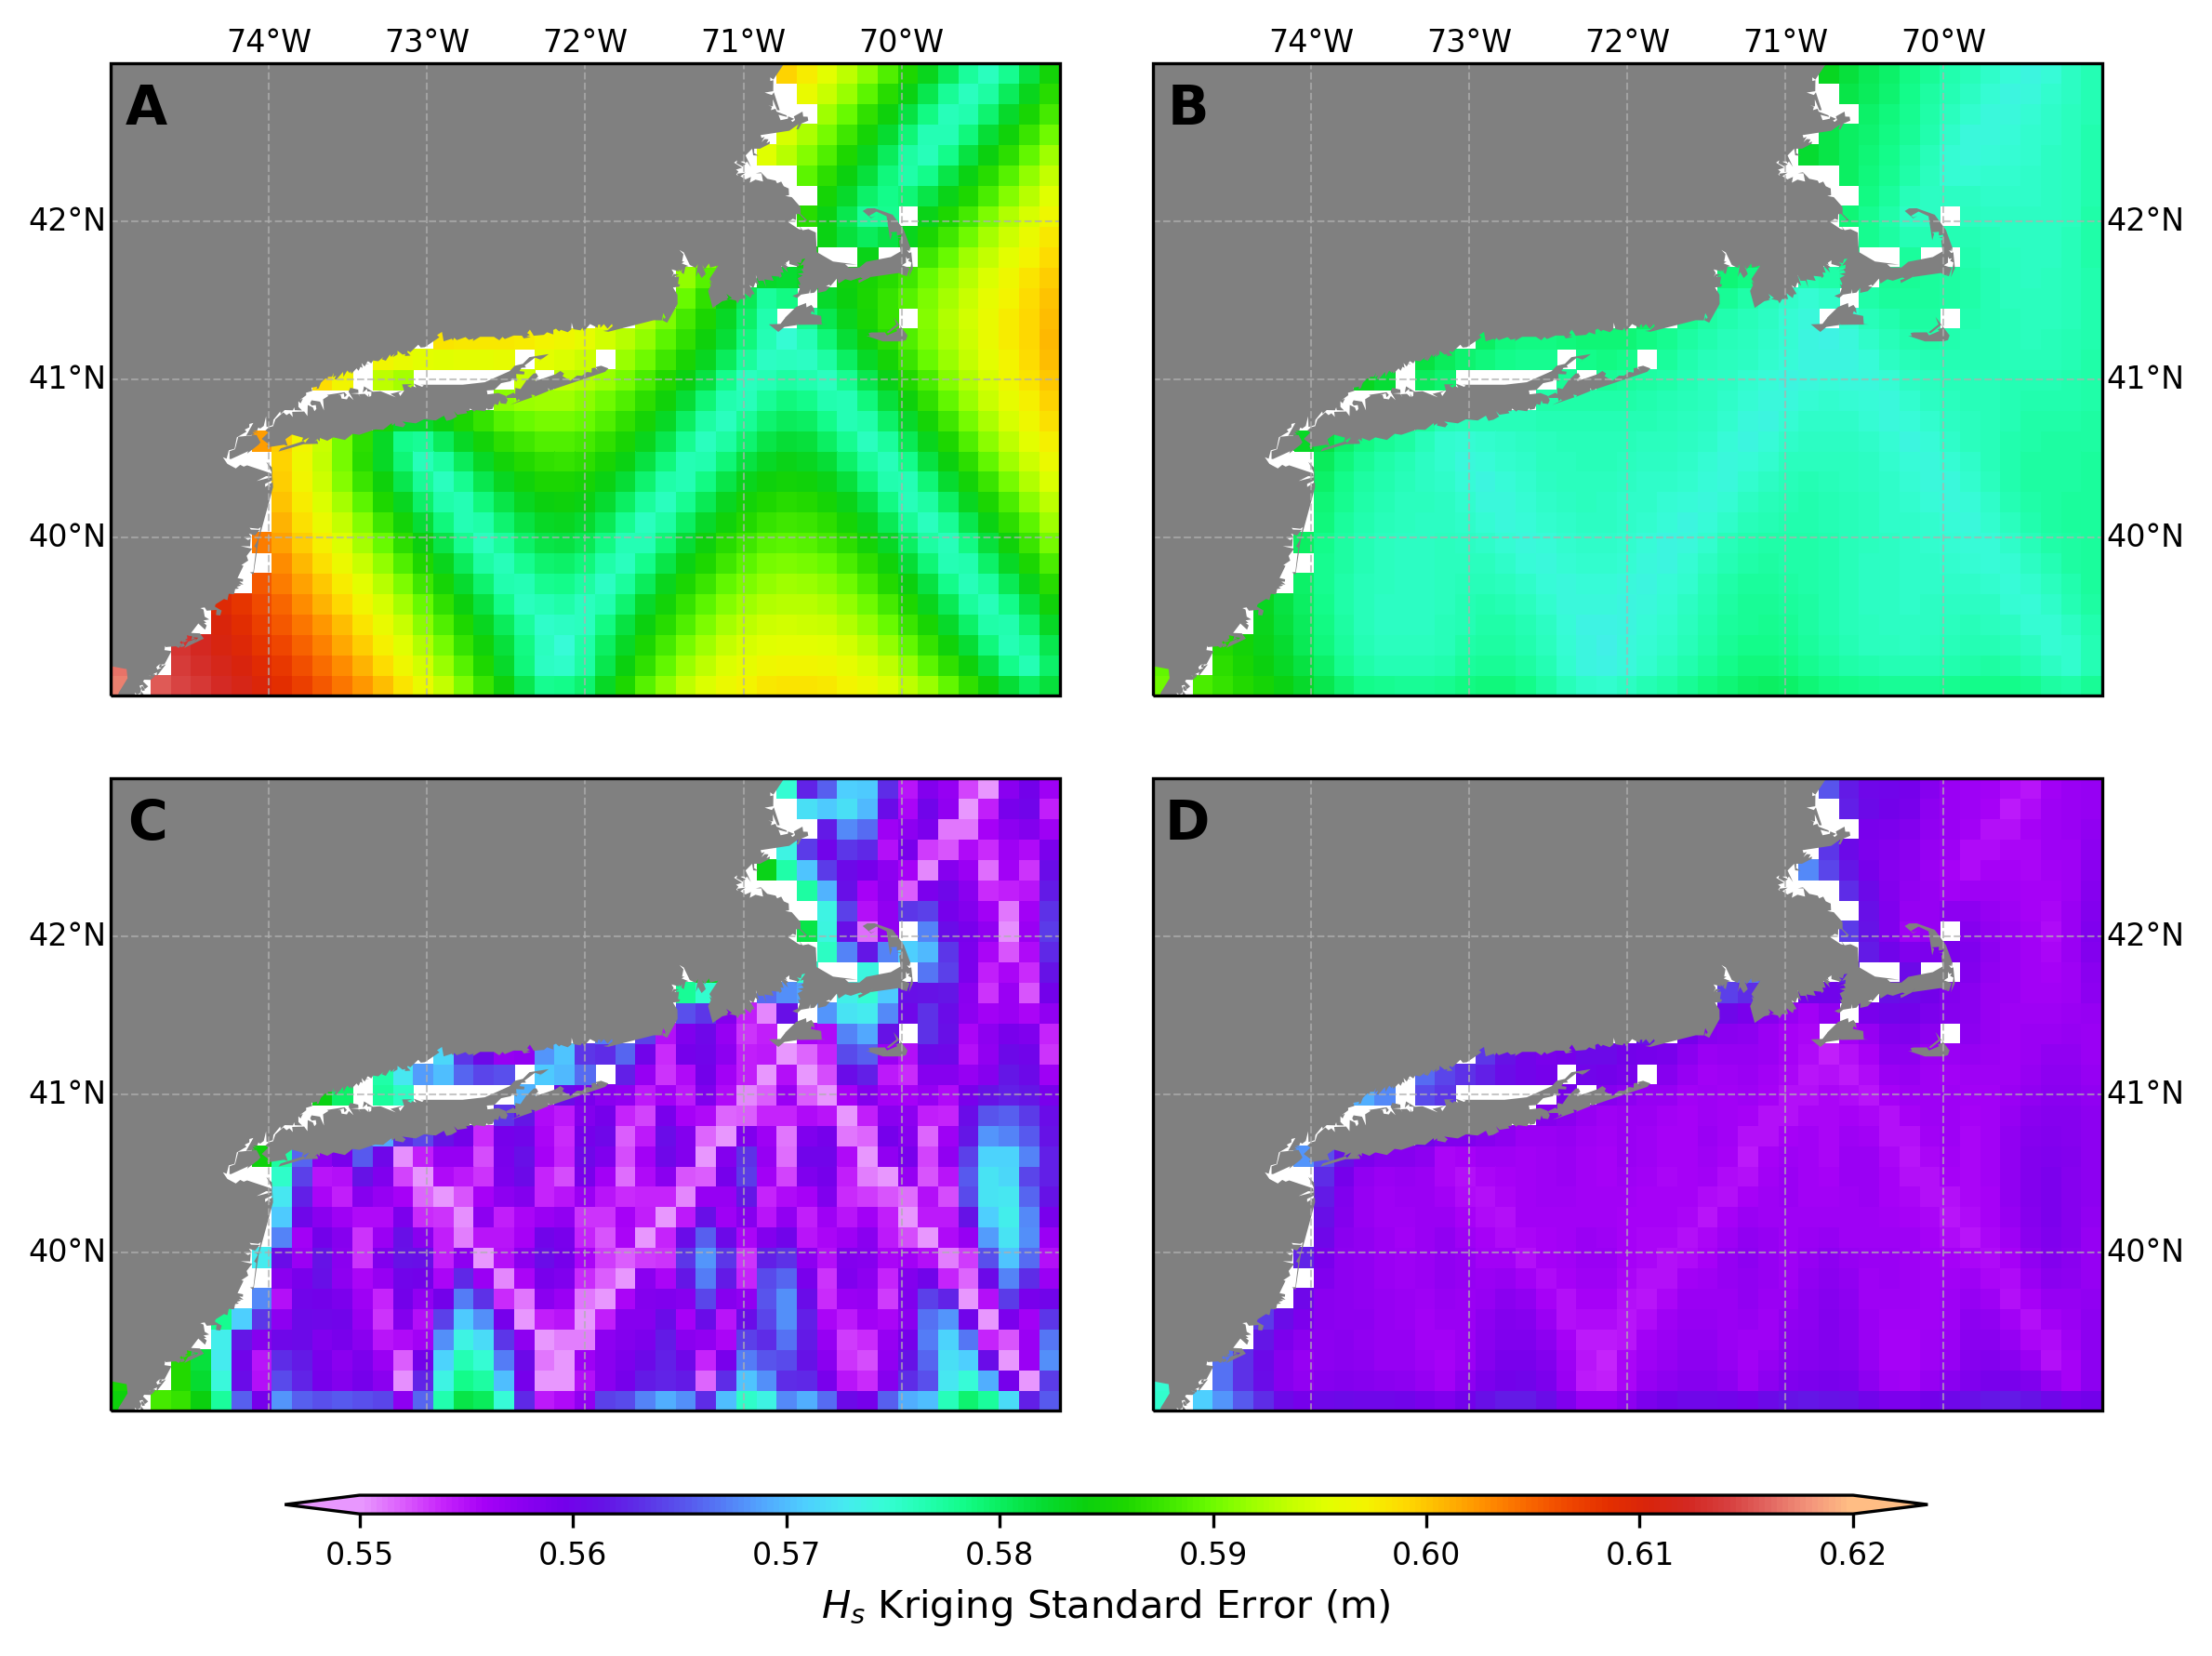
\includegraphics[width=0.95\linewidth]{Figures/Chapter5/kriging_mapping_error_w19_1.png}
%\decoRule
\caption{SWH kriging standard error maps for the 2019 winter using data from (A) Jason 3,  (B) Jason 3 and SARAL-AltiKa, (C) Jason 3, SARAL-AltiKa and Sentinel 3 and (D) all altimeters.}
\label{fig:kriging_error}
\end{figure}


The diurnal sampling bias \cite{Ahsbahs2020, Barthelmie2003} also needs to be considered, especially for the WS and consequently, offshore wind energy estimation. In Section~\ref{diurnal_variability}, we showed that there is substantial diurnal variability in locations with a distance less than 40 kilometers from the closest coast, based on observations from buoys, which record the WS every 10 minutes. In contrast, satellites generally pass over a region at specific hours during the day. Three of the five altimeters used in this study,  SARAL-Altika, Sentinel 3 A and B, pass over SNE at certain hours. These are the hours of the ascending and the descending tracks. Specifically, SARAL-AltiKa's ascending tracks pass at 6:00-6:30 AM and the descending tracks twelve hours later. Sentinel 3 ascending tracks pass at 9:00-9:30 PM and the descending tracks at 11:00-11:30 AM. Jason 3 and Cryosat 2 pass at irregular times over SNE. Indeed, each cycle or subcycle begins one hour later than the previous one. 



\begin{figure}[H]
\centering
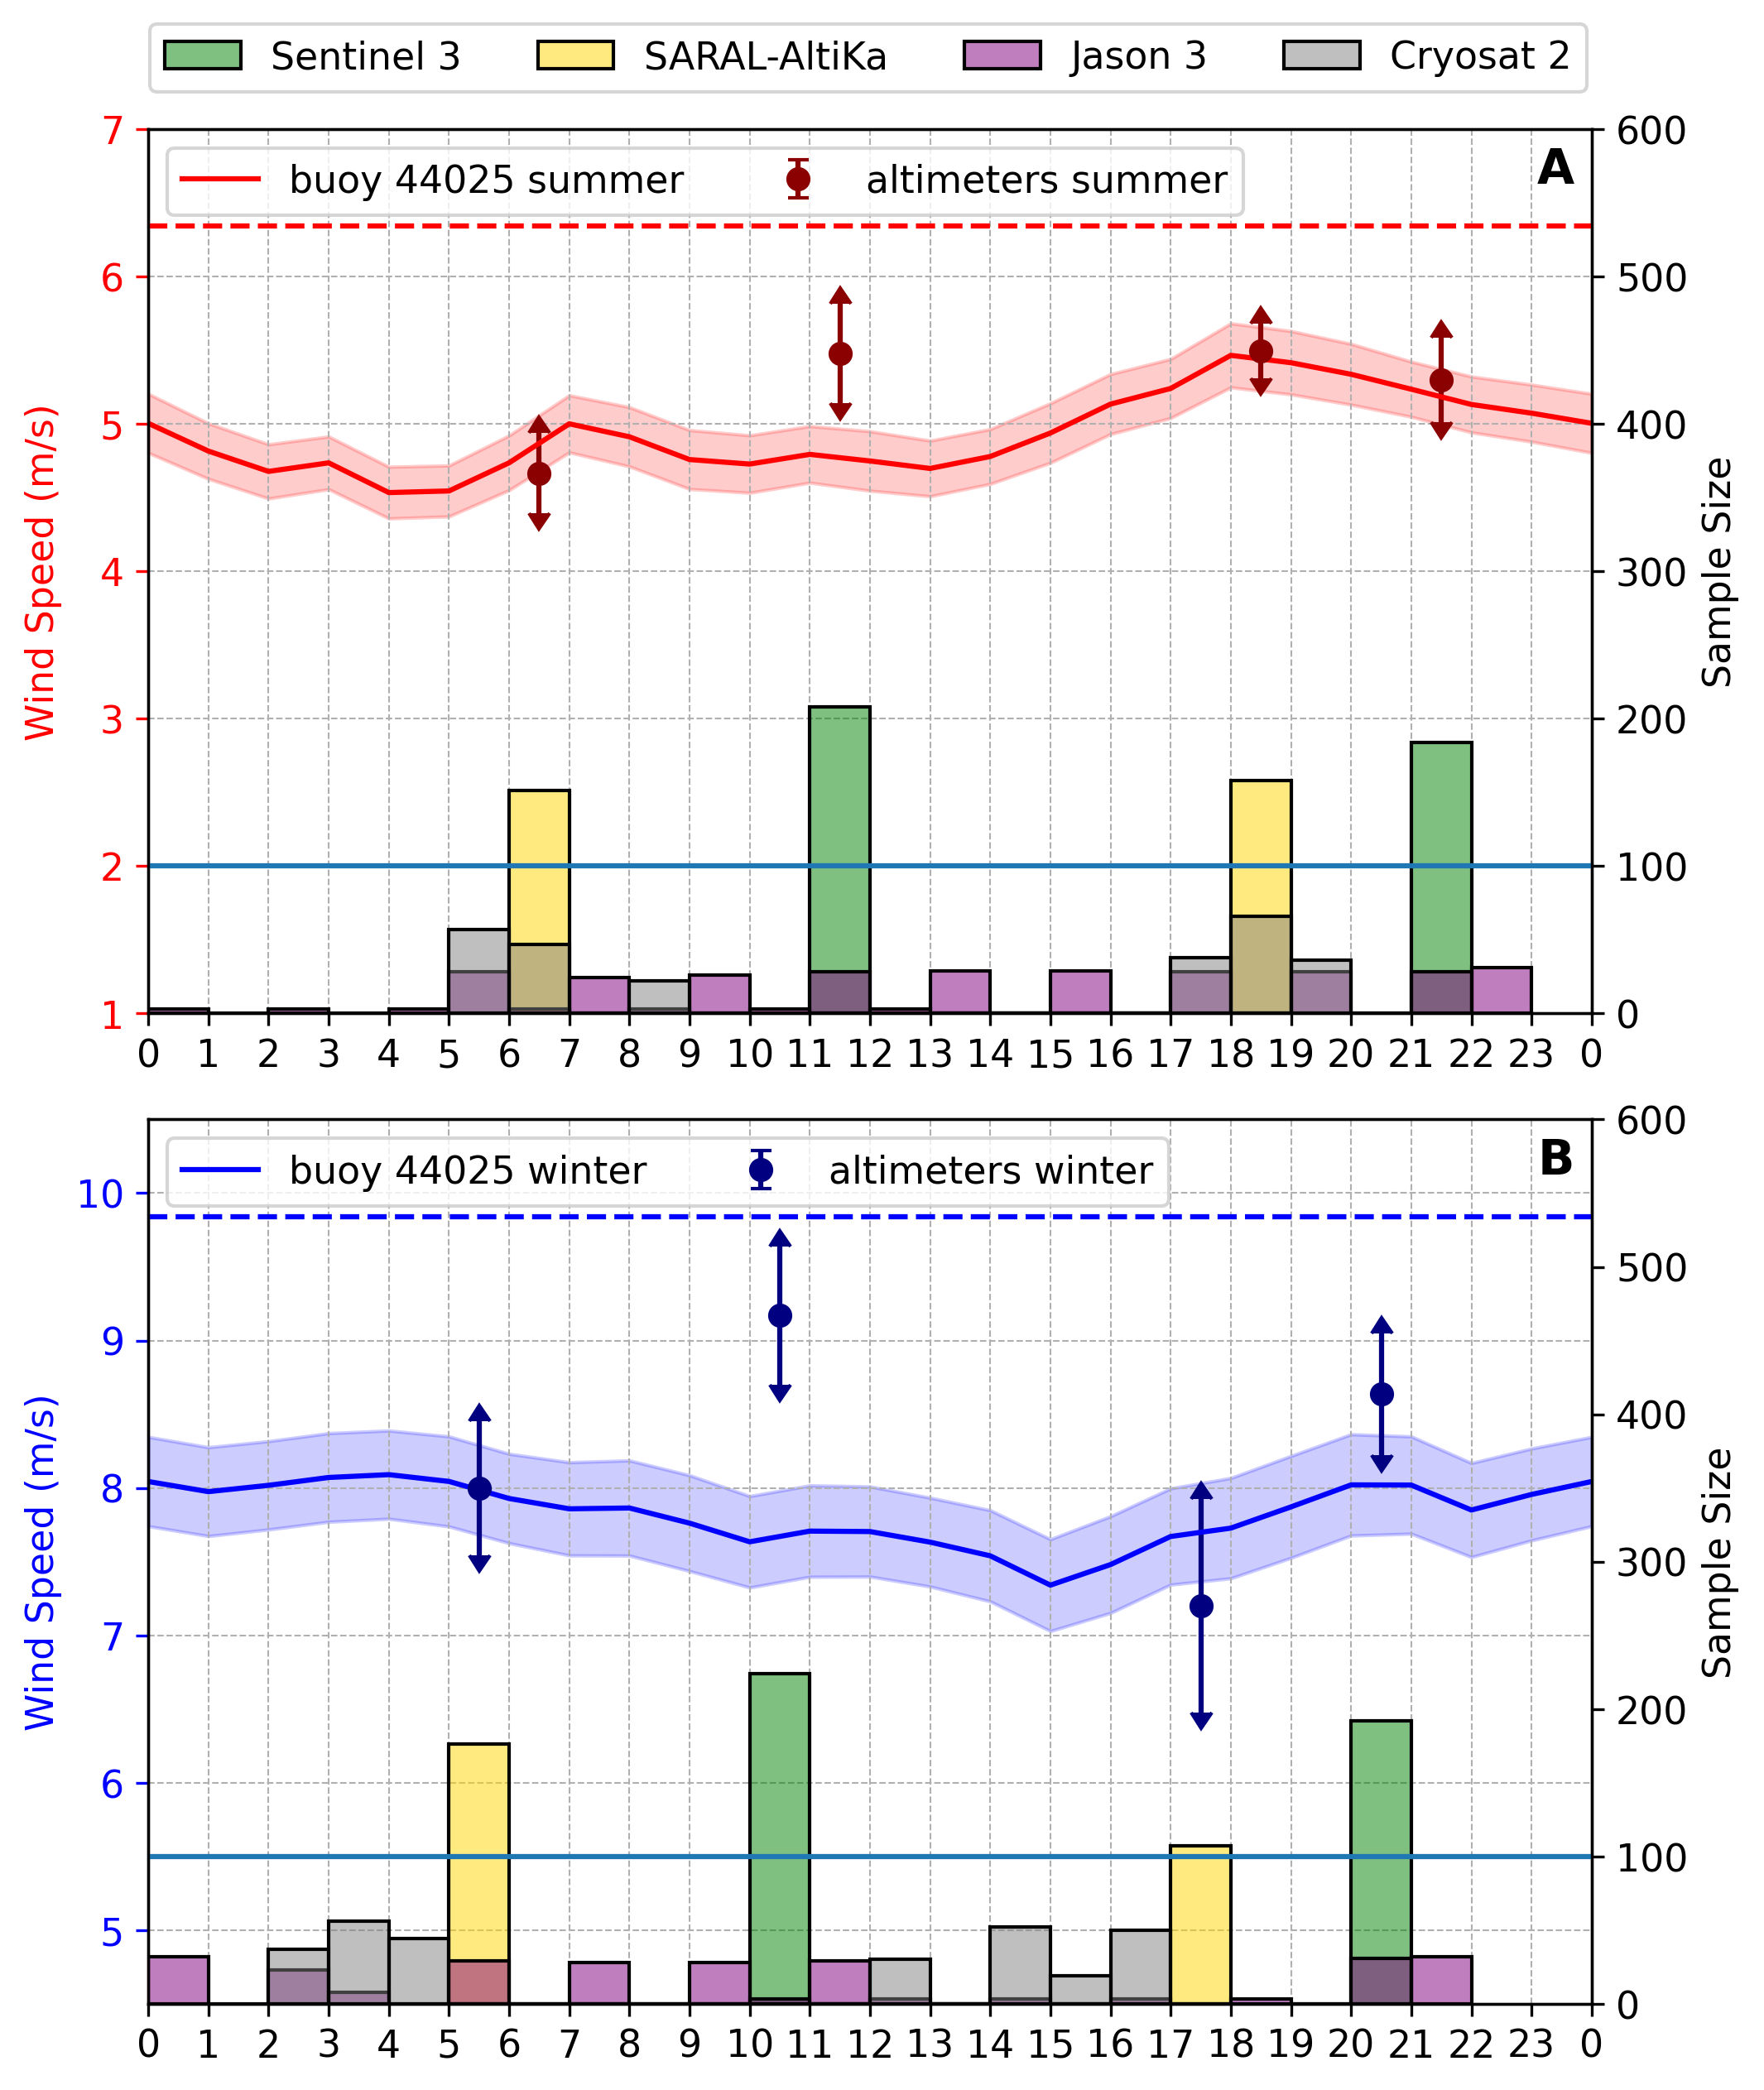
\includegraphics[width=0.75\linewidth]{Figures/Chapter5/alt_buoy44025_2019_diur_bias4.png}
%\decoRule
\caption{A visualization of the diurnal bias due to altimeter sampling frequency compared with buoy 44025 for the summer (A) and winter (B) seasons. A straight horizontal blue line was added to display the sample size limit (100) of altimeter observations for the calculation of the average WS value that represents specific hours. The dashed horizontal lines were added to display the minimum available buoy observations for each hour (534).}
\label{fig:diurnal_bias_wind2019}
\end{figure}




A summary of this description and comparison with buoy data is presented in Figure~\ref{fig:diurnal_bias_wind2019}. The histograms represent the altimeter sample size, and a light blue horizontal line is added to visualize the sample size limit for the comparison with buoy observations. We selected a limit of 100 altimeter observations with a maximum distance of 1 degree from buoy 44025. The average and confidence intervals are represented with red dots and arrows for the summer and blue for the winter season. The 1-degree distance is relatively large, but we wanted to have enough observations to compare with over 500 observations per hour from the buoy represented by the blue and red dashed lines. The average WS from altimeters are generally close to the buoy average except for the observations representing the descending Sentinel 3 track. This difference is more significant during winter, and it could be partly attributed to the spatial and temporal limitations previously mentioned. Besides, the SARAL-AltiKa descending track captures the highest WS values at the buoy 44025 location during summer. On the other hand, altimeters' tracks do not coincide with the lowest WS values observed between 5:00 to 6:00 AM by buoy 44025. During winter, both the buoy maximum at 4:00 AM and the minimum WS at 3:00 PM are represented only by a small number of Cryosat 2 and Jason 3 observations. Figure~\ref{fig:diurnal_bias_wind2019} is also essential because it depicts the temporal gaps we need to fill with other sensors that measure the WS like scatterometers or SAR to reduce the uncertainty.





\label{Chapter5} % For referencing the chapter elsewhere, use \ref{Chapter5}